\documentclass[11pt,a4paper]{article}
\usepackage{float}
\usepackage{subfig}
\usepackage{dirtree}
\usepackage{wrapfig}
\usepackage{amsmath}
\usepackage{textcomp}
\usepackage{csquotes}
\usepackage{graphicx}
\usepackage{listings}
\usepackage{enumitem}
\usepackage{dirtytalk}
\usepackage[bottom]{footmisc}
\usepackage[linktoc=none]{hyperref}
\usepackage[backend=biber]{biblatex}
\addbibresource{bibliography.bib}
\usepackage[dvipsnames,table]{xcolor}
\usepackage[colorinlistoftodos]{todonotes}
\usepackage[justification=centering]{caption}
\usepackage[ruled, linesnumbered]{algorithm2e}
\usepackage[a4paper, portrait, margin=1.2in]{geometry}
\usepackage[framed, autolinebreaks, useliterate]{mcode}
\hypersetup{
	colorlinks=true,
	linkcolor=blue,
	filecolor=magenta,      
	urlcolor=blue,
}
\lstset{aboveskip=\medskipamount}
\DontPrintSemicolon
\begin{document}
\begin{center}
	\Large\textbf{Ensemble of Images and Point Clouds Classification}\\
	\vspace{0.2cm}
	\large{Computational Intelligence and Deep Learning final project}\\
	\large{Prof. Beatrice Lazzerini}\\
	\large{Alessandro Renda, PhD}\\
	\vspace{1.0cm}
	\large\textit{Rambod Rahmani}\\
	\vspace{0.2cm}
	\normalsize{Msc. in Artificial Intelligence and Data Engineering}\\
	\vspace{1.0cm}
	\today
\end{center}
\vspace{1cm}
\setcounter{tocdepth}{2}
\tableofcontents

\newpage
\section{Introduction}
The project aims to perform object classification by means of Convolutional Neural Networks using RGB images and 3D point clouds. The dataset of interest is ShapeNet: a richly-annotated, large-scale dataset of 3D shapes and images \cite{shapenet2015}.\\
The classification task is a multiclass one and aims to classify everyday life objects. The idea for this project came from the notion of \textit{Sensor Fusion}.
\subsection{Sensor Fusion}
Autonomous mobile robots \cite{s18082730} operate by sensing and perceiving their surrounding environment to make accurate driving decisions. A combination of several different sensors such as LiDAR, radar, ultrasound sensors and cameras are utilized to sense the surrounding environment of autonomous vehicles. These heterogeneous sensors simultaneously capture various physical attributes of the environment. Such multimodality and redundancy of sensing need to be positively utilized for reliable and consistent perception of the environment through sensor data fusion.\\
\textbf{The project was inspired by the notion of \textit{Sensor fusion}}\footnote{\url{https://en.wikipedia.org/wiki/Sensor_fusion}}: the process of combining sensor data or data derived from disparate sources such that the resulting information has less uncertainty than would be possible when these sources were used individually. The term \textit{uncertainty reduction} in this case can mean more accurate, more complete, or more dependable.\\
\\
Each sensor type, or “modality,” has inherent strengths and weaknesses. Radars are very strong at accurately determining distance and speed — even in challenging weather conditions — but can’t read street signs or “see” the color of a stoplight. Cameras do very well reading signs or classifying objects, such as pedestrians, bicyclists or other vehicles. However, they can easily be blinded by dirt, sun, rain, snow or darkness. LiDARs can accurately detect objects, but they don’t have the range or affordability of cameras or radar. Long story short, the following infographic summarizes it quite well:
\begin{figure}[H]
    \centering
    \includegraphics[scale=0.08]{imgs/sensor-fusion.jpg}
\end{figure}
\noindent
Laser Imaging Detection and Ranging (LiDAR) \cite{s21123992} and camera sensors are two of the most used sensors for this task since they can accurately provide important features such as target's depth and shape.\\
\\
\textbf{The idea behind the project was therefore to develop deep learning models to perform classification on both RGB images and point clouds.}\\
\\
The following details the tasks executed during the development of the project. The following major tasks and sub-tasks were identified in the planning stage:
\begin{itemize}
    \item Task 0: State-of-the-art Deep Learning on 3D Point Clouds:
    \item Task 1: Dataset Preprocessing
        \begin{itemize}
            \item The Dataset: ShapeNet
            \item Merge 3D models and renders
            \item Organize data in macro-categories
            \item Dataset balancing
            \item Stratified K-Fold Cross Validation
        \end{itemize}
    \item Task 2: Training from scratch
        \begin{itemize}
            \item Experiments
            \begin{itemize}
                \item RGB Images
                \item 3D Point Clouds
            \end{itemize}
        \end{itemize}
    \item Task 3: State-of-the-art
        \begin{itemize}
            \item Experiments
            \begin{itemize}
                \item RGB Images
                \item 3D Point Clouds
            \end{itemize}
        \end{itemize}
    \item Task 4: Ensemble
\end{itemize}
The project was developed using \texttt{Python 3.9.10} and \texttt{TensorFlow 2.8.0-rc0}. For each task a dedicated Jupyter Notebook is provided. Instead of running the code relaying on Google Colab resources, I preferred using my own hardware\footnote{NVIDIA RTX A5000.} due to the large size of the dataset ($\sim 50$ GiB).\\
\\
A shared Google drive was created containing:
\begin{itemize}
    \item the Jupyter Notebooks associated to each task;
    \item an additional Jupyter Notebook named \texttt{Scratchbook.ipynb} containing some trial and error implementation attempts of the different pieces of code found in the notebooks associated to each task;
    \item this \texttt{.pdf} file containing the final project report with high resolution images;
    \item models checkpoints;
\end{itemize}
The original dataset was not uploaded due to size limitations but can be downloaded directly from the ShapeNet organization website as detailed in \nameref{section:dataset-preprocessing}.

\newpage
\section{Task 0: State-of-the-art Deep Learning on 3D Point Clouds}
A point cloud is a set of points defined in a 3D metric space. Point clouds have become one of the most significant data format for 3D representation. Its gaining increased popularity as a result of increased availability of acquisition devices, such as LiDAR sensors, as well as increased application in areas such as robotics, autonomous driving, augmented and virtual reality. Deep learning is now the most powerful tool for data processing in computer vision, becoming the most preferred technique for tasks such as classification, segmentation, and detection. \textbf{While deep learning techniques are mainly applied to data with a structured grid, point cloud, on the other hand, is unstructured.}\\
The unstructuredness of point clouds makes use of deep learning for its processing directly very challenging. Earlier approaches overcome this challenge by preprocessing the point cloud into a structured grid format at the cost of increased computational cost or lost of depth information. Recently, however, many state-of-the-arts deep learning techniques that directly operate on point cloud are being developed. \cite{9127813}
\subsection{Deep Learning methods for 3D point clouds}
We can distinguish three main applications of deep learning to 3D point clouds:
\begin{figure}[H]
    \centering
    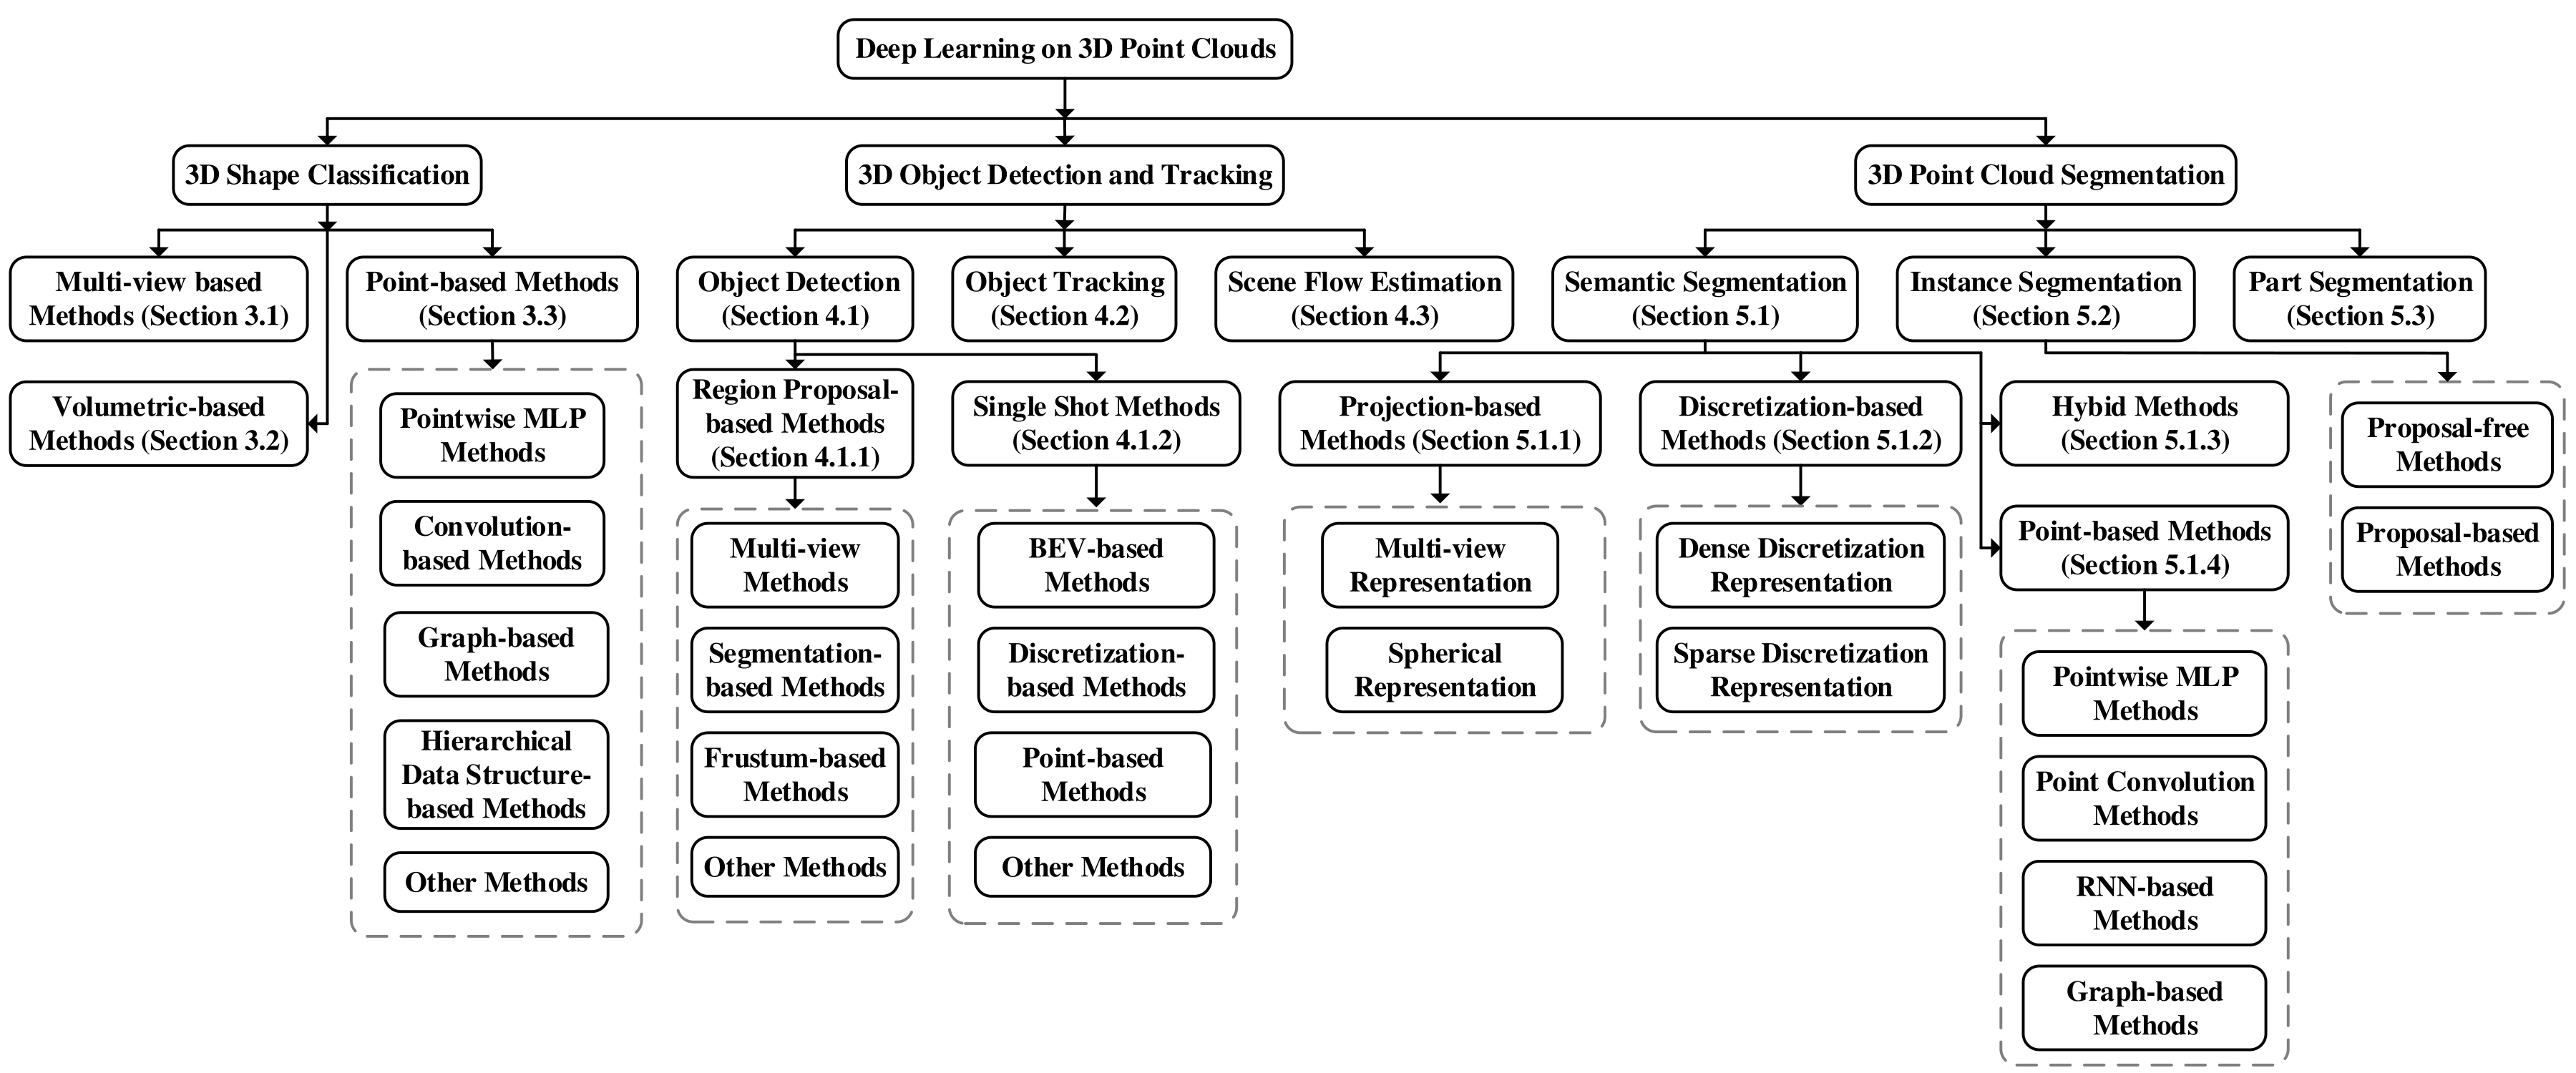
\includegraphics[scale=0.7]{imgs/pointcloud-deeplearning-taxonomy.jpg}
    \caption{A taxonomy of deep learning methods for 3D point clouds. \cite{abs200106280}}
\end{figure}
\noindent
\begin{itemize}
    \item \textbf{3D Shape Classification}: Methods for this task usually learn the embedding of each point first and then extract a global shape embedding from the whole point cloud using an aggregation method. Classification is finally achieved by feeding the global embedding into several fully connected layers. According to the data type of input for neural networks, existing 3D shape classification methods can be divided into \textit{multi-view based}, \textit{volumetric-based} and \textit{point-based} methods.
    \begin{figure}[H]
        \centering
        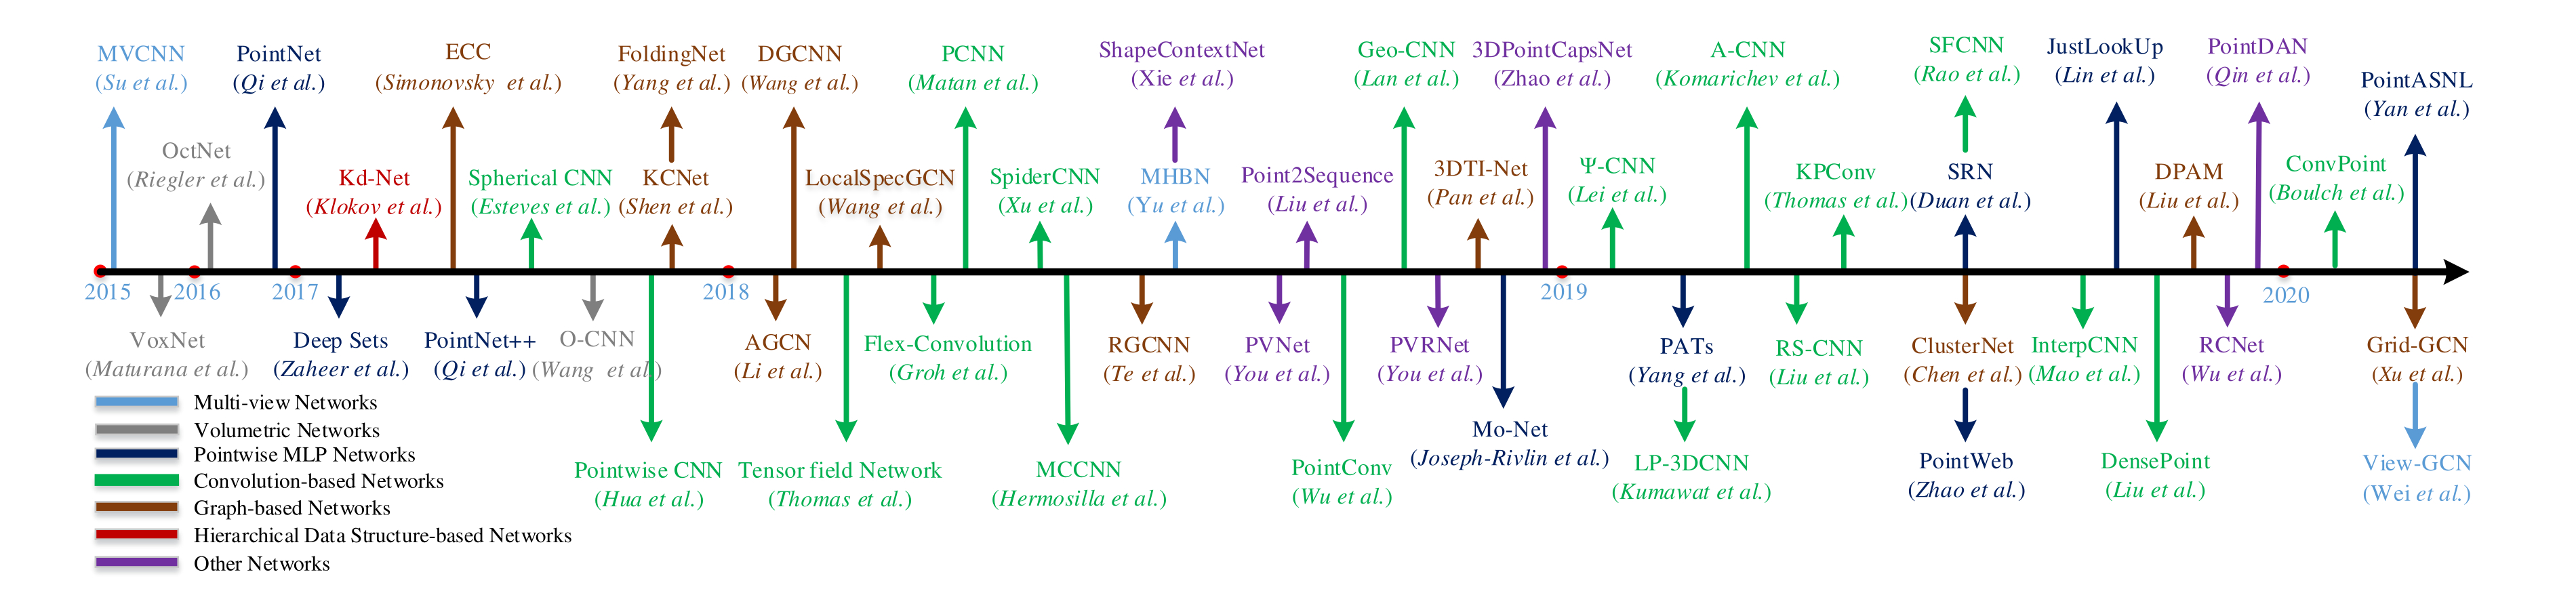
\includegraphics[scale=0.7]{imgs/pointcloud-classification-methods.jpg}
        \caption{Chronological overview of 3D shape classification methods}
    \end{figure}
    \item \textbf{3D Object Detection and Tracking}: A typical 3D object detector takes the point cloud of a scene as its input and produces an oriented 3D bounding box around each detected object. Similar to object detection in images, 3D object detection methods can be divided into two categories: \textit{region proposal-based} and \textit{single shot methods}.
    \begin{figure}[H]
        \centering
        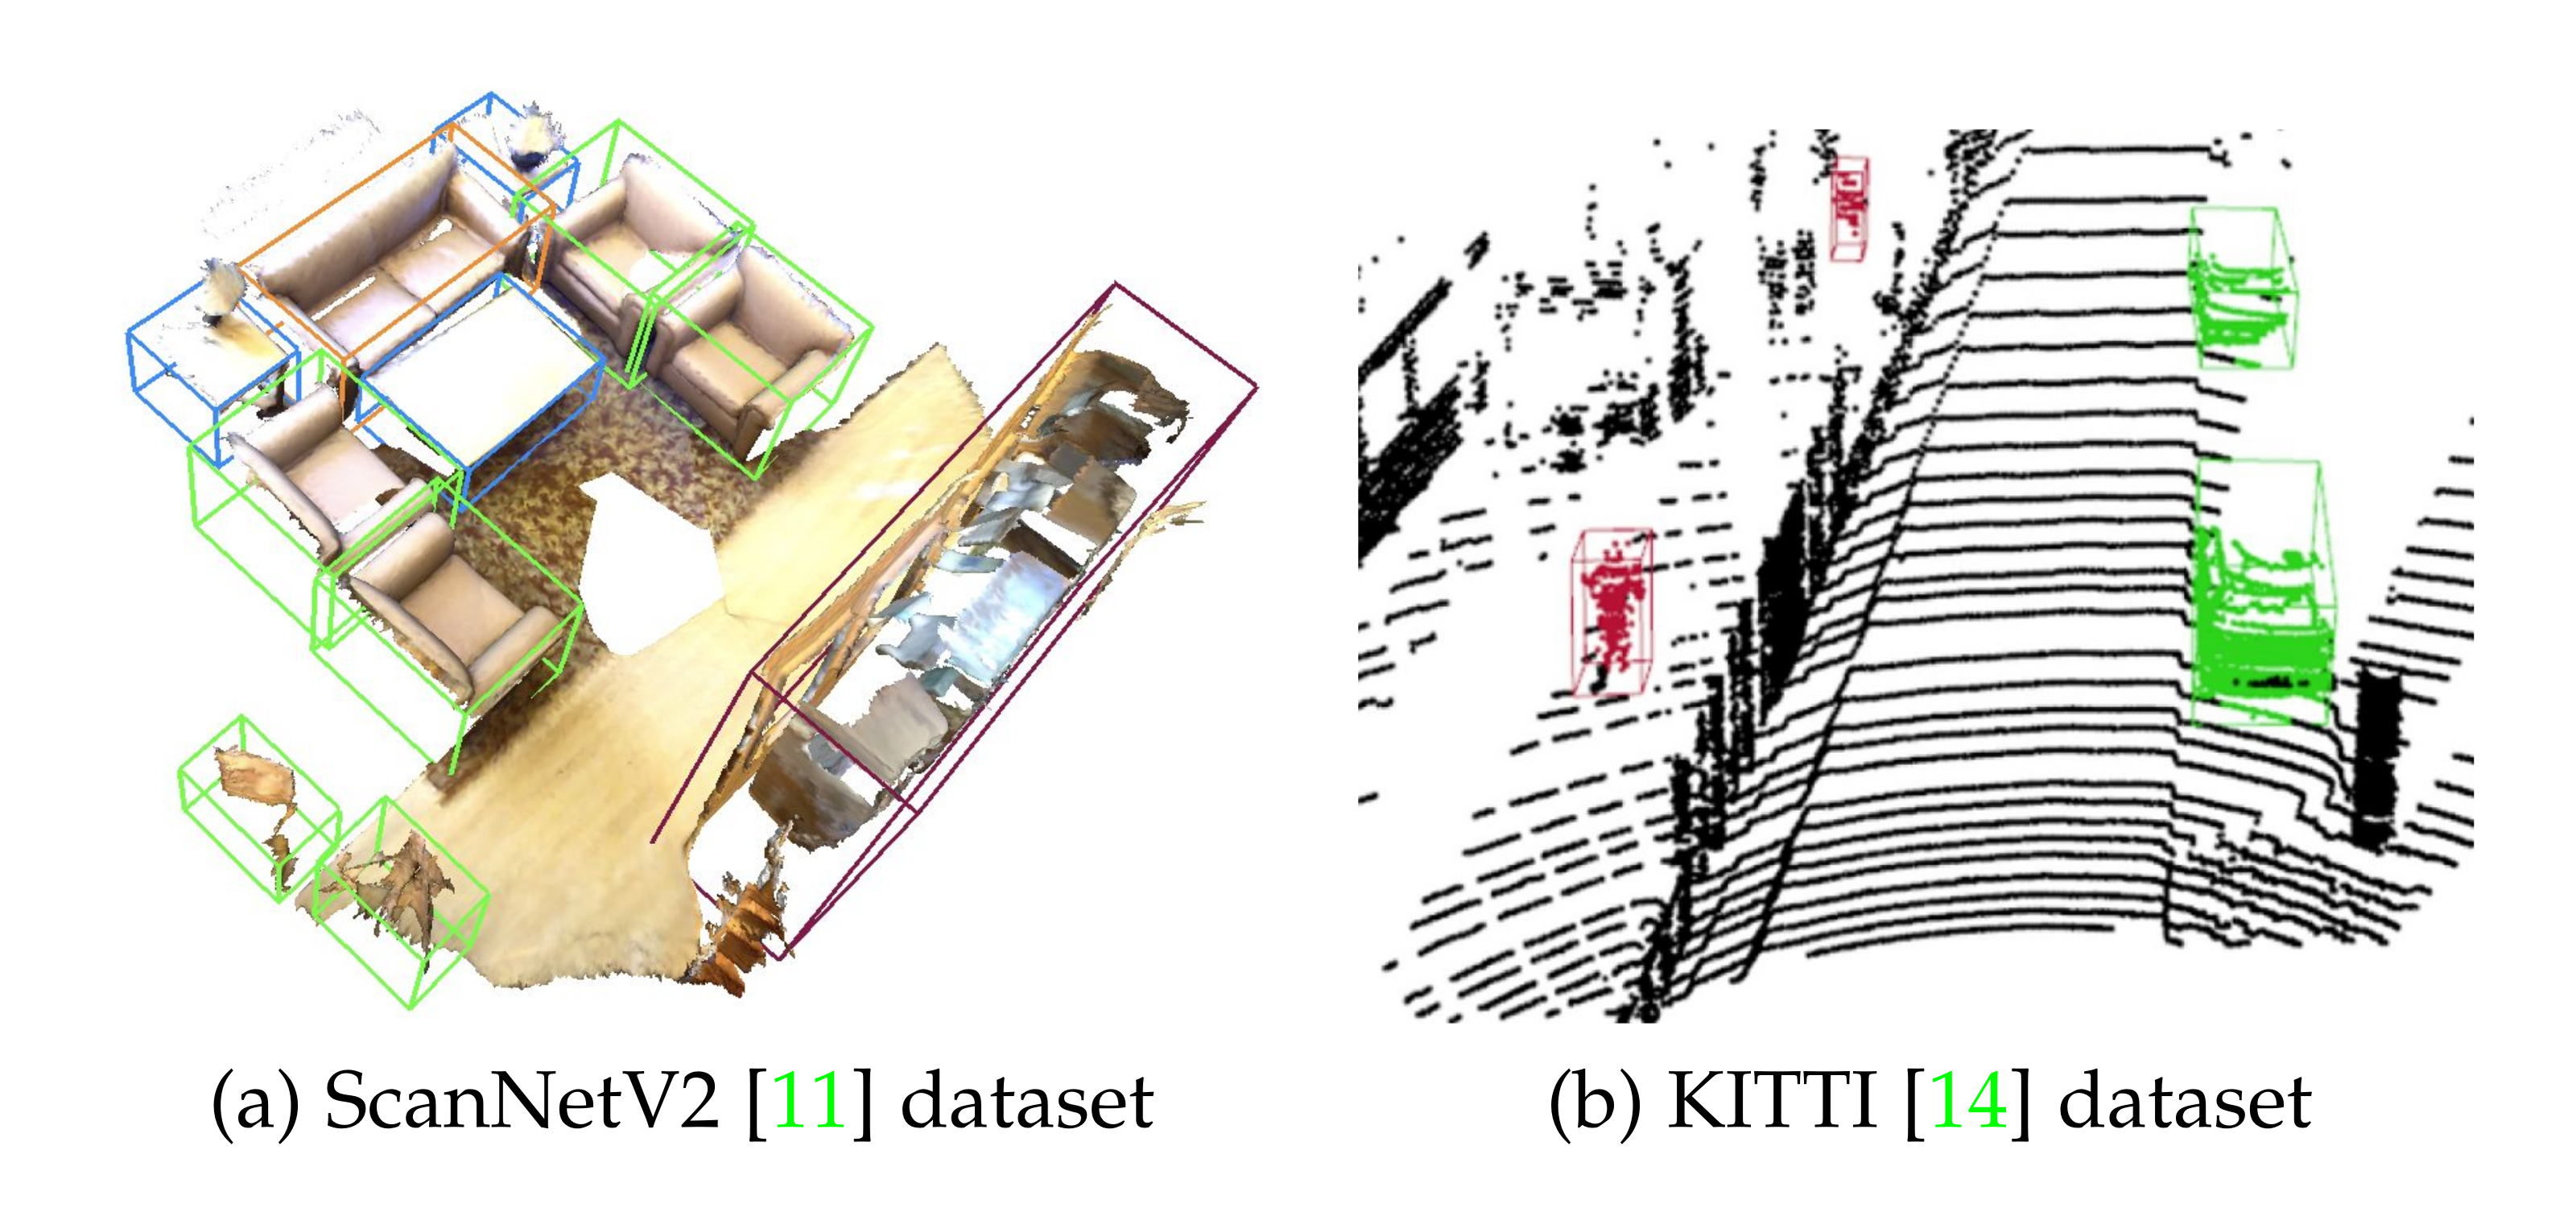
\includegraphics[scale=1.2]{imgs/pointcloud-object-detection.jpg}
    \end{figure}
    \begin{figure}[H]
        \centering
        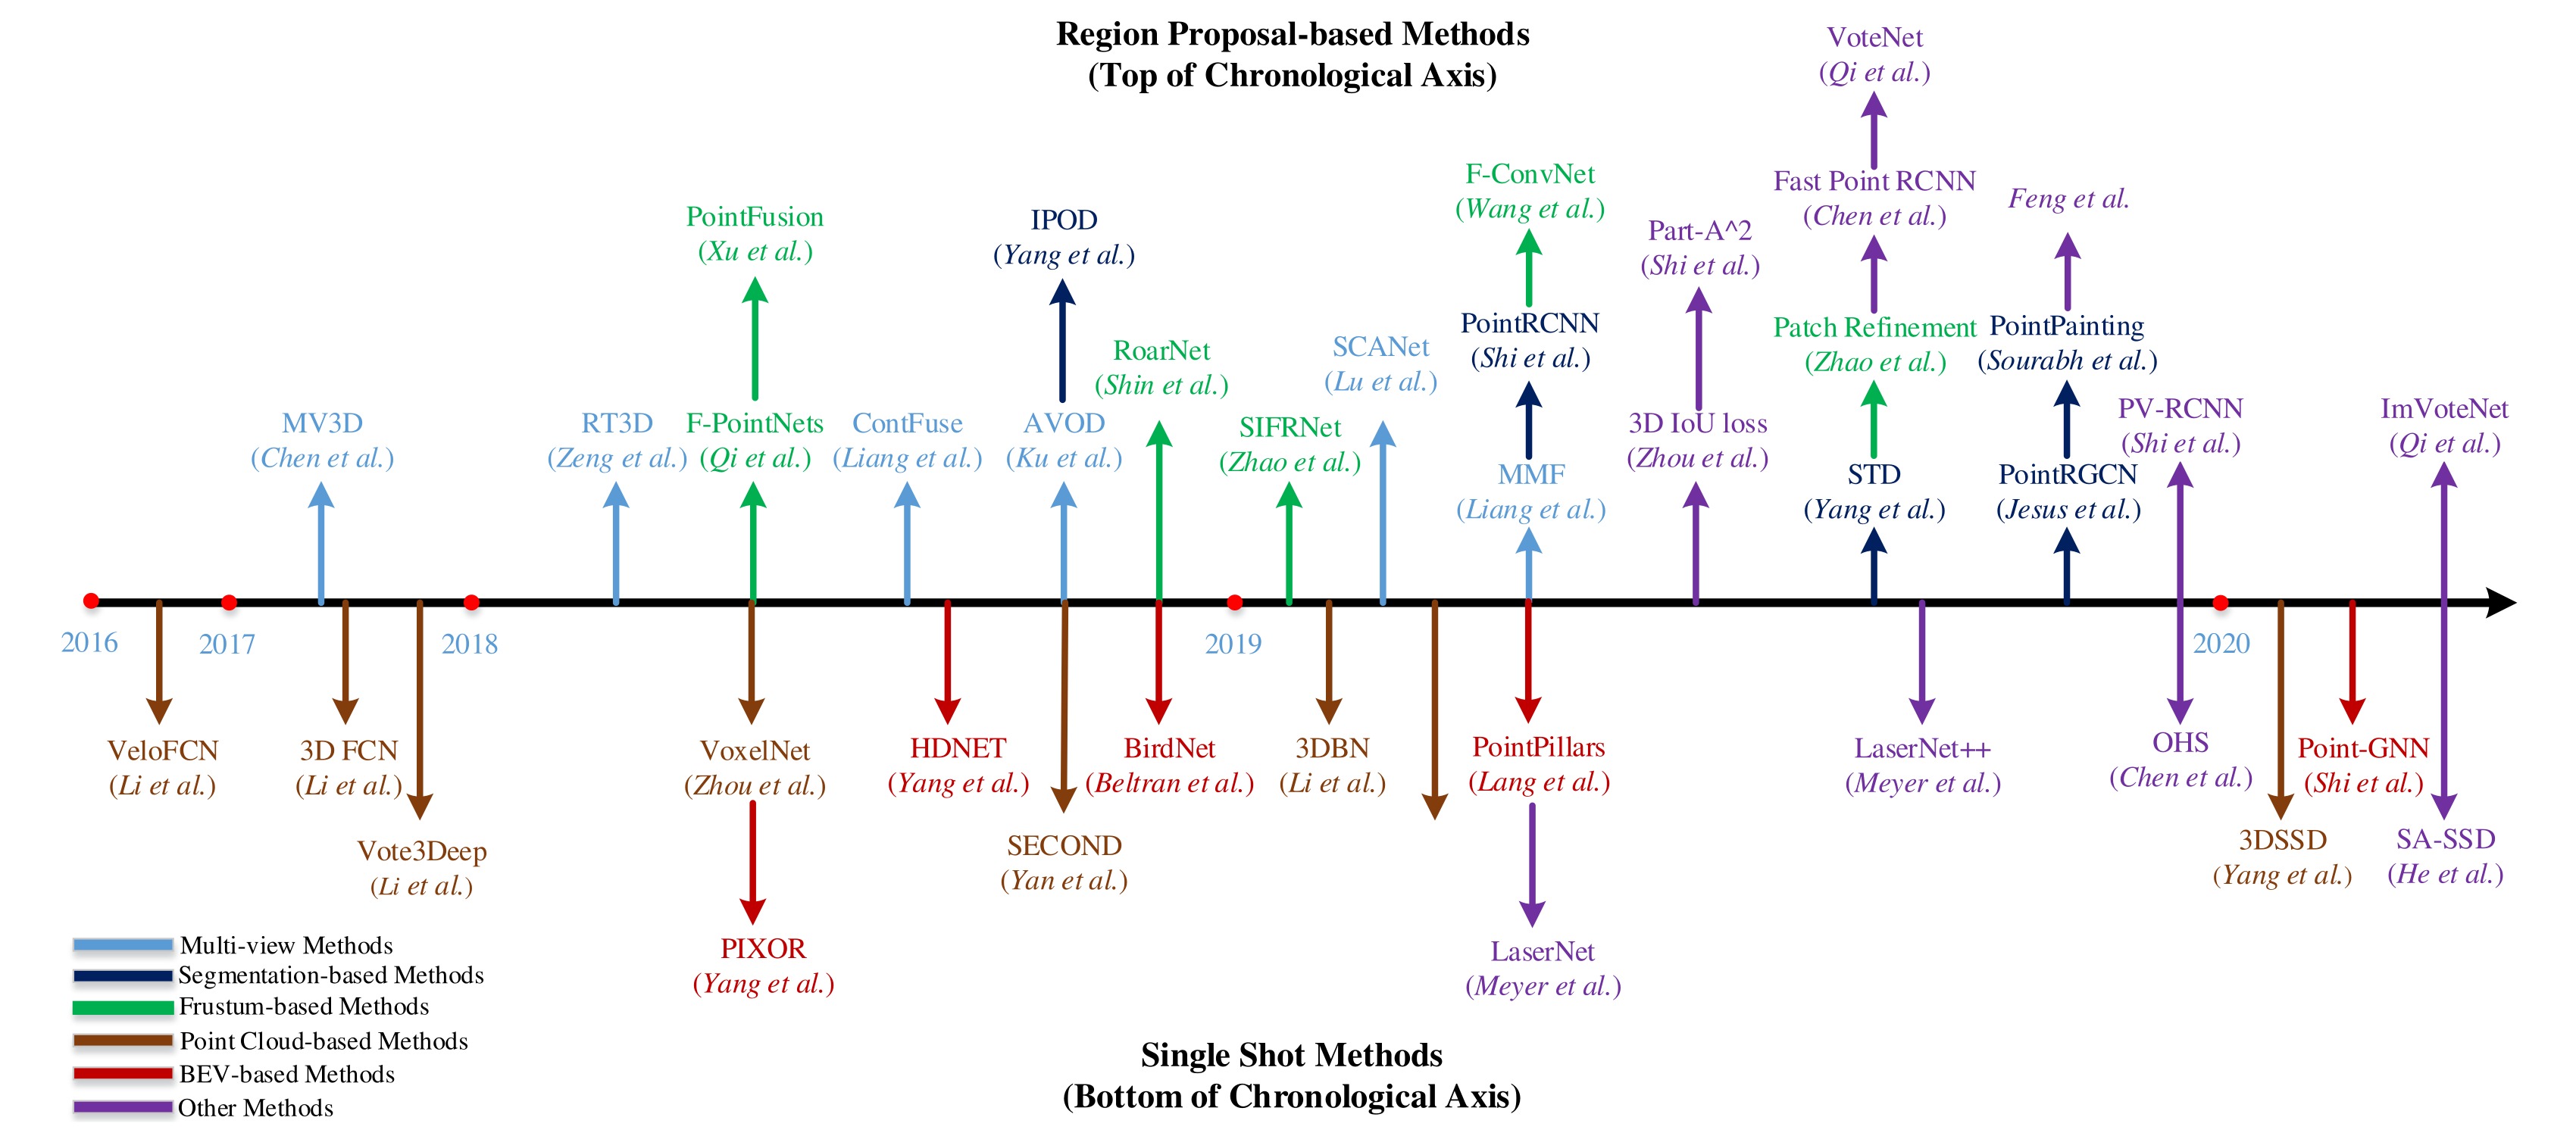
\includegraphics[scale=0.7]{imgs/pointcloud-object-detection-methods.jpg}
        \caption{Chronological overview of 3D object detection methods}
    \end{figure}
    \item \textbf{3D Point Cloud Segmentation}: 3D point cloud segmentation requires the understanding of both the global geometric structure and the fine-grained details of each point. According to the segmentation granularity, 3D point cloud segmentation methods can be classified into three categories: \textit{semantic segmentation} (scene level), \textit{instance segmentation} (object level) and \textit{part segmentation} (part level).
    \begin{figure}[H]
        \centering
        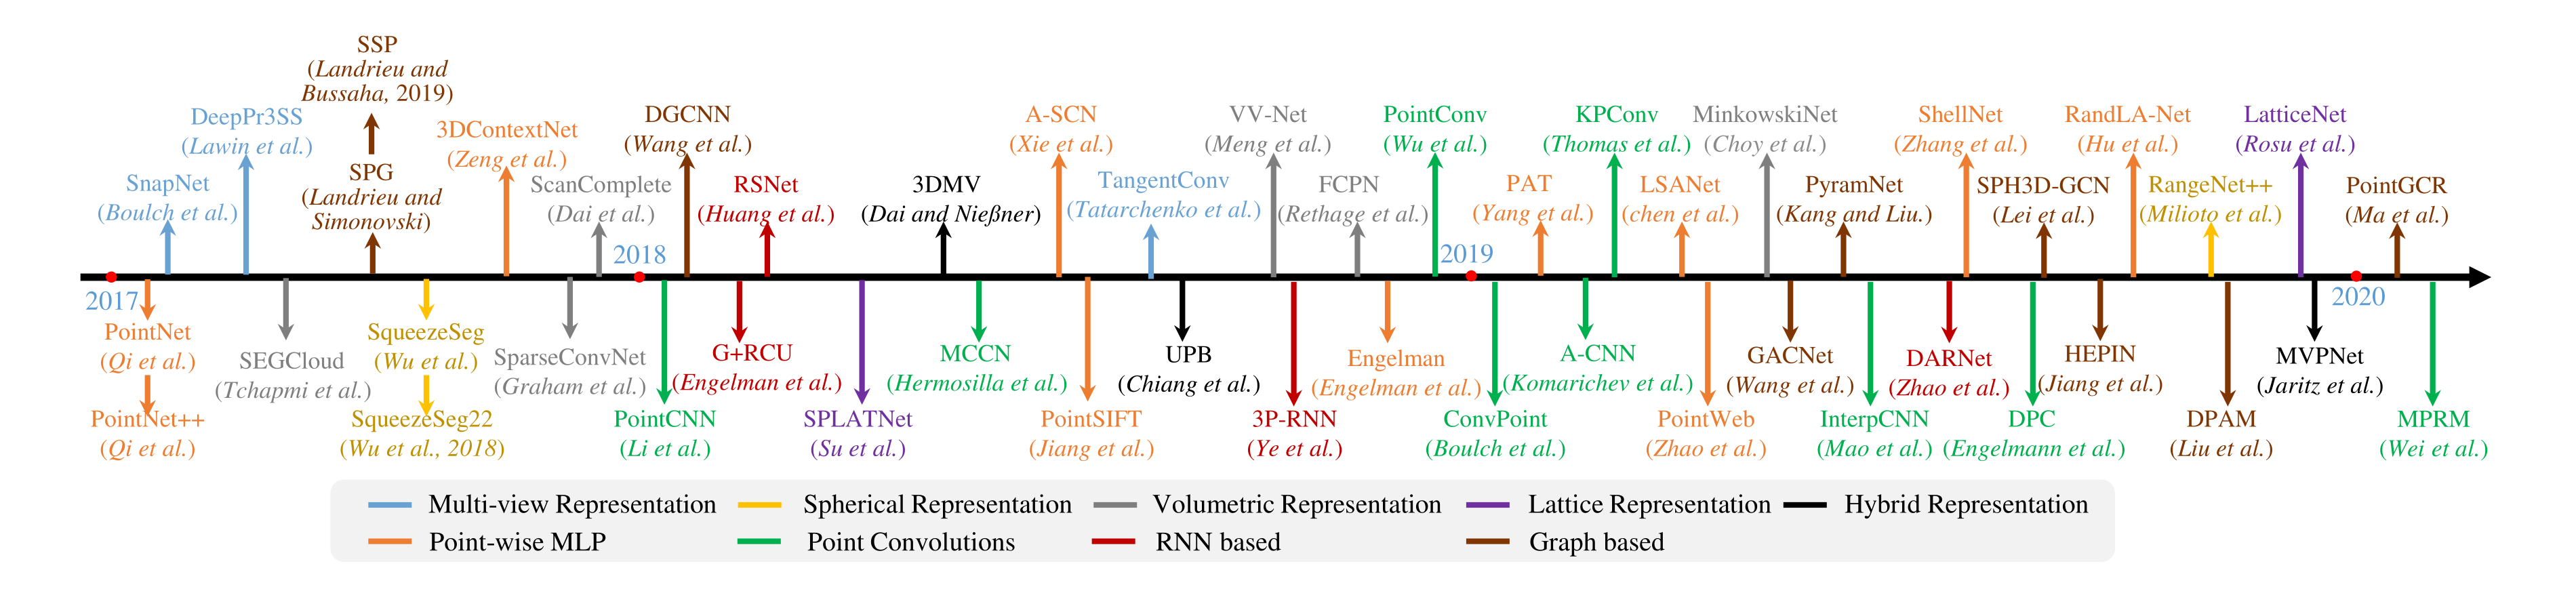
\includegraphics[scale=0.7]{imgs/pointcloud-segmentation-methods.jpg}
        \caption{Chronological overview of 3D semantic segmentation methods}
    \end{figure}
\end{itemize}
\subsection{Challenges of deep learning on point clouds}
Applying deep learning on 3D point cloud data comes with many challenges. Some of these challenges include occlusion which is caused by cluttered scene or blind side; noise/outliers which are unintended points; points misalignment e.t.c. How- ever, the more pronounced challenges when it comes to application of deep learning on point clouds can be categorized into the following:
\begin{figure}[H]
    \centering
    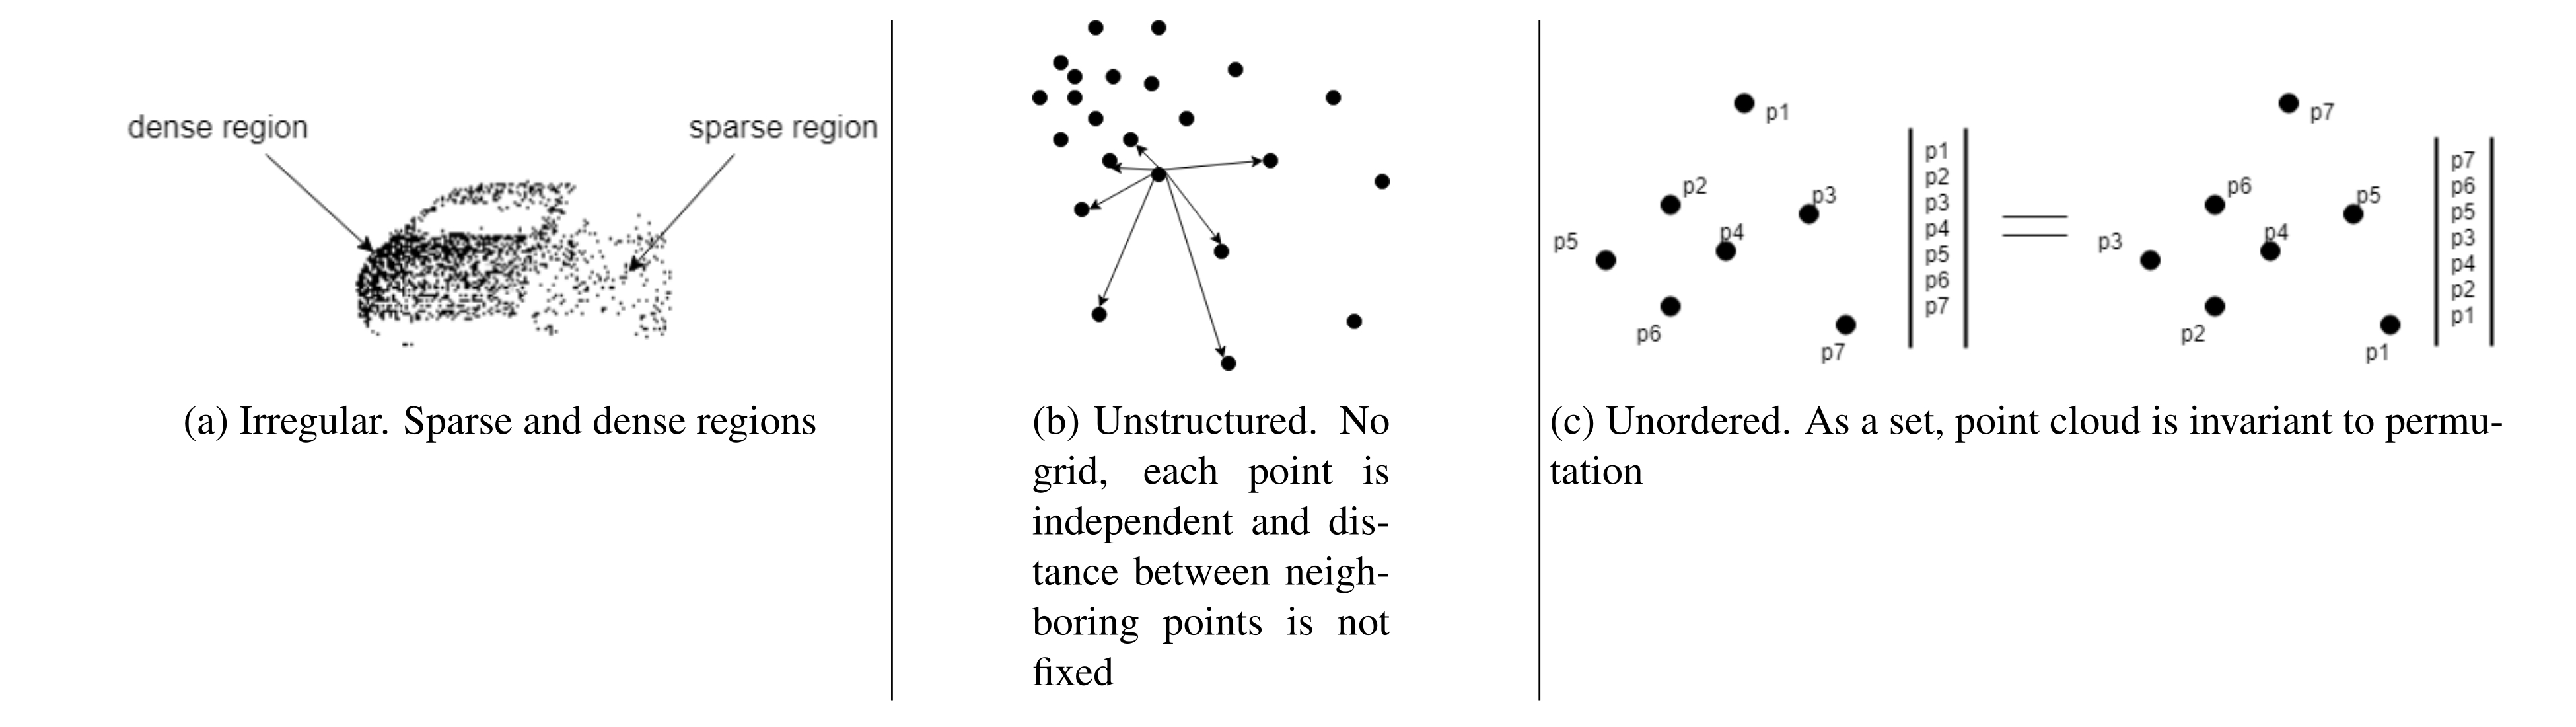
\includegraphics[scale=0.7]{imgs/pointcloud-deeplearning-challenges.jpg}
    \caption{Challenges of deep learning on point clouds}
\end{figure}
\begin{itemize}
    \item \textbf{Irregularity}: point cloud data is irregular, meaning, the points are not evenly sampled accross the different regions of an object/scene, so some regions could have dense points while others sparse points. These can be seen in figure 5a.
    \item \textbf{Unstructured}: point cloud data is not on a regular grid. Each point is scanned independently and its distance to neighboring points is not always fixed, in contrast, pixels in images are represented on a 2-dimension grid, and spacing between two adjacent pixels is always fixed.
    \item \textbf{Unorderdness}: Point cloud of a scene is the set of points (usually represented by $(XYZ)$) obtained around the objects in the scene and are usually stored as a list in a file. As a set, the order in which the points are stored does not change the scene represented. The unordered nature of point sets is shown in figure 5c.
\end{itemize}
These properties of point cloud are very challenging for deep learning, especially convolutional neural networks (CNN). These is because convolutional neural networks are based on convolution operation which is performed on a data that is ordered, regular and on a structured grid. Early approaches overcome these challenges by converting the point cloud into a structured grid format. However, recently researchers have been developing approaches that directly uses the power of deep learning on raw point cloud, taking away the need for preprocessing.

\newpage
\section{Task 1: Dataset Preprocessing}
\label{section:dataset-preprocessing}
The implementation of what is described in this section can be found in the Jupyter Notebook named \texttt{Task1-Preprocessing.ipynb}.\\
\\
For classification, there are two types of datasets: synthetic datasets, and real-world datasets. Objects in the synthetic datasets are complete, without any occlusion and background. In contrast, objects in the real-world datasets are occluded at different levels and some objects are contaminated with background noise. The decision was made to use a synthetic dataset containing 3D models and the correlated rendered images obtained by applying textures. The following random sample is useful to immediately clarify the nature of the data we will be dealing with:
\begin{figure}[H]
    \centering
    \subfloat[\centering 3D Object]{{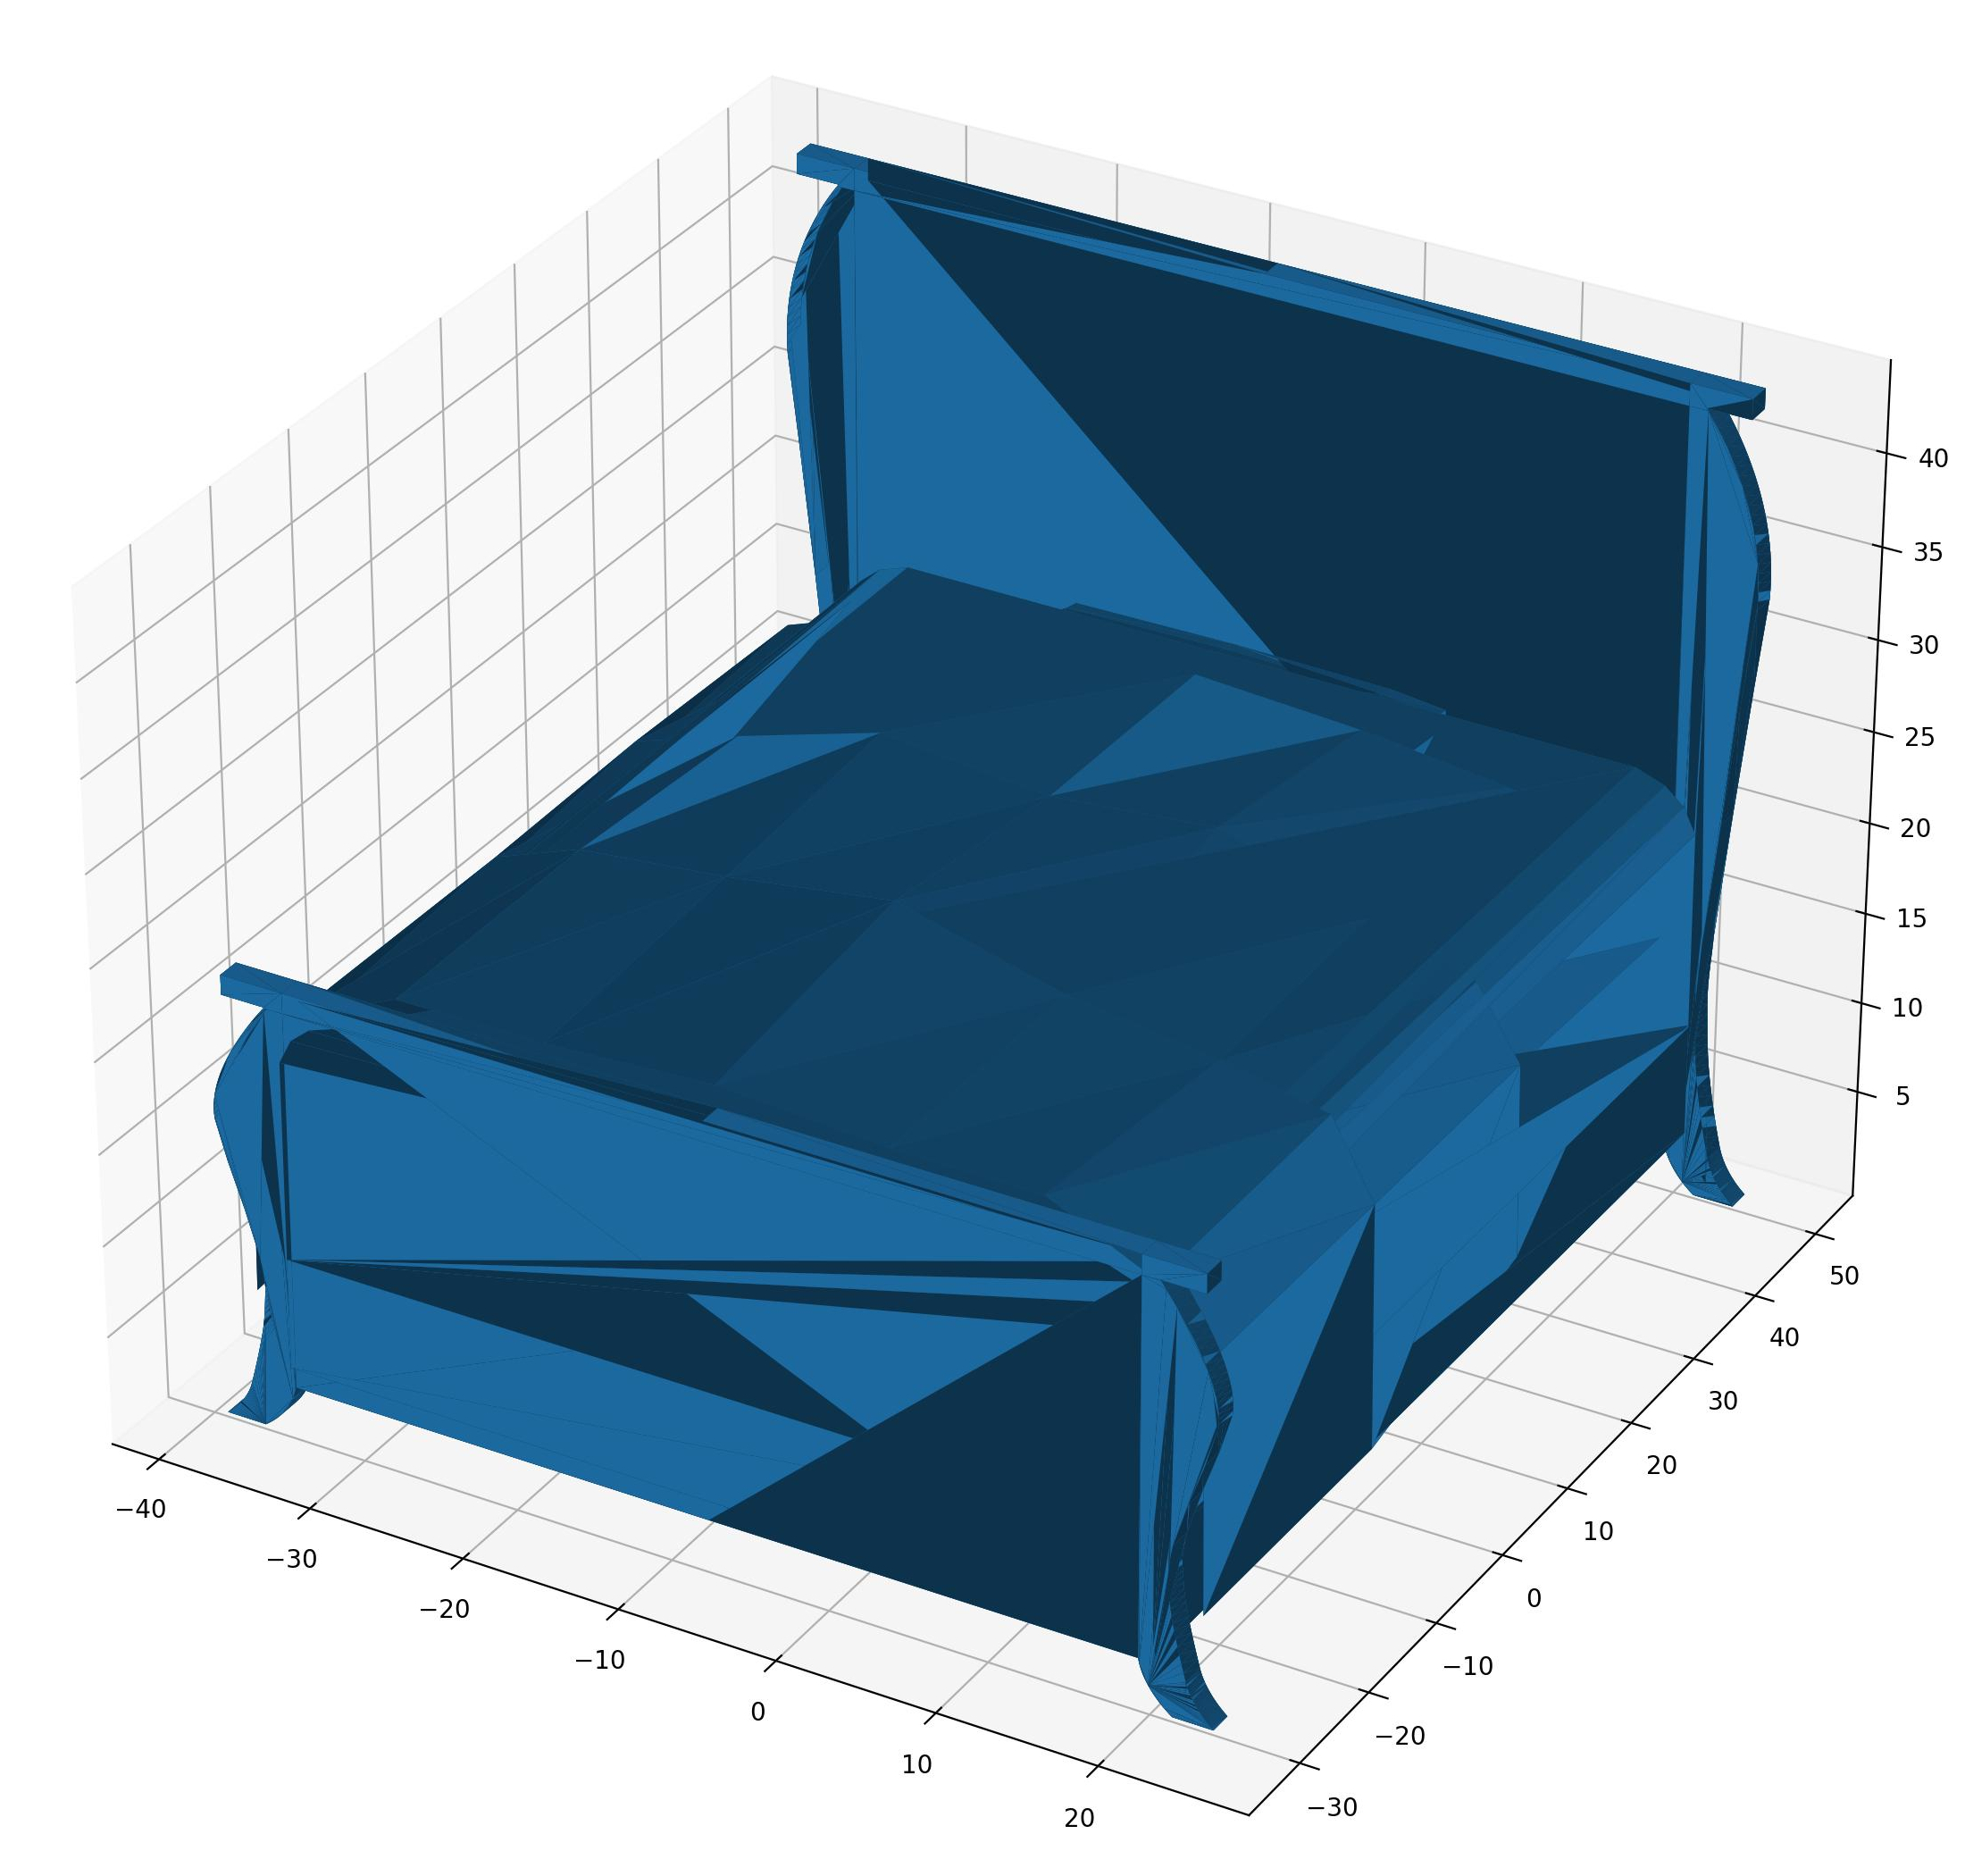
\includegraphics[scale=0.26]{imgs/example-mesh-trisurf.jpg} }}
    \qquad
    \subfloat[\centering Sampled Point Cloud]{{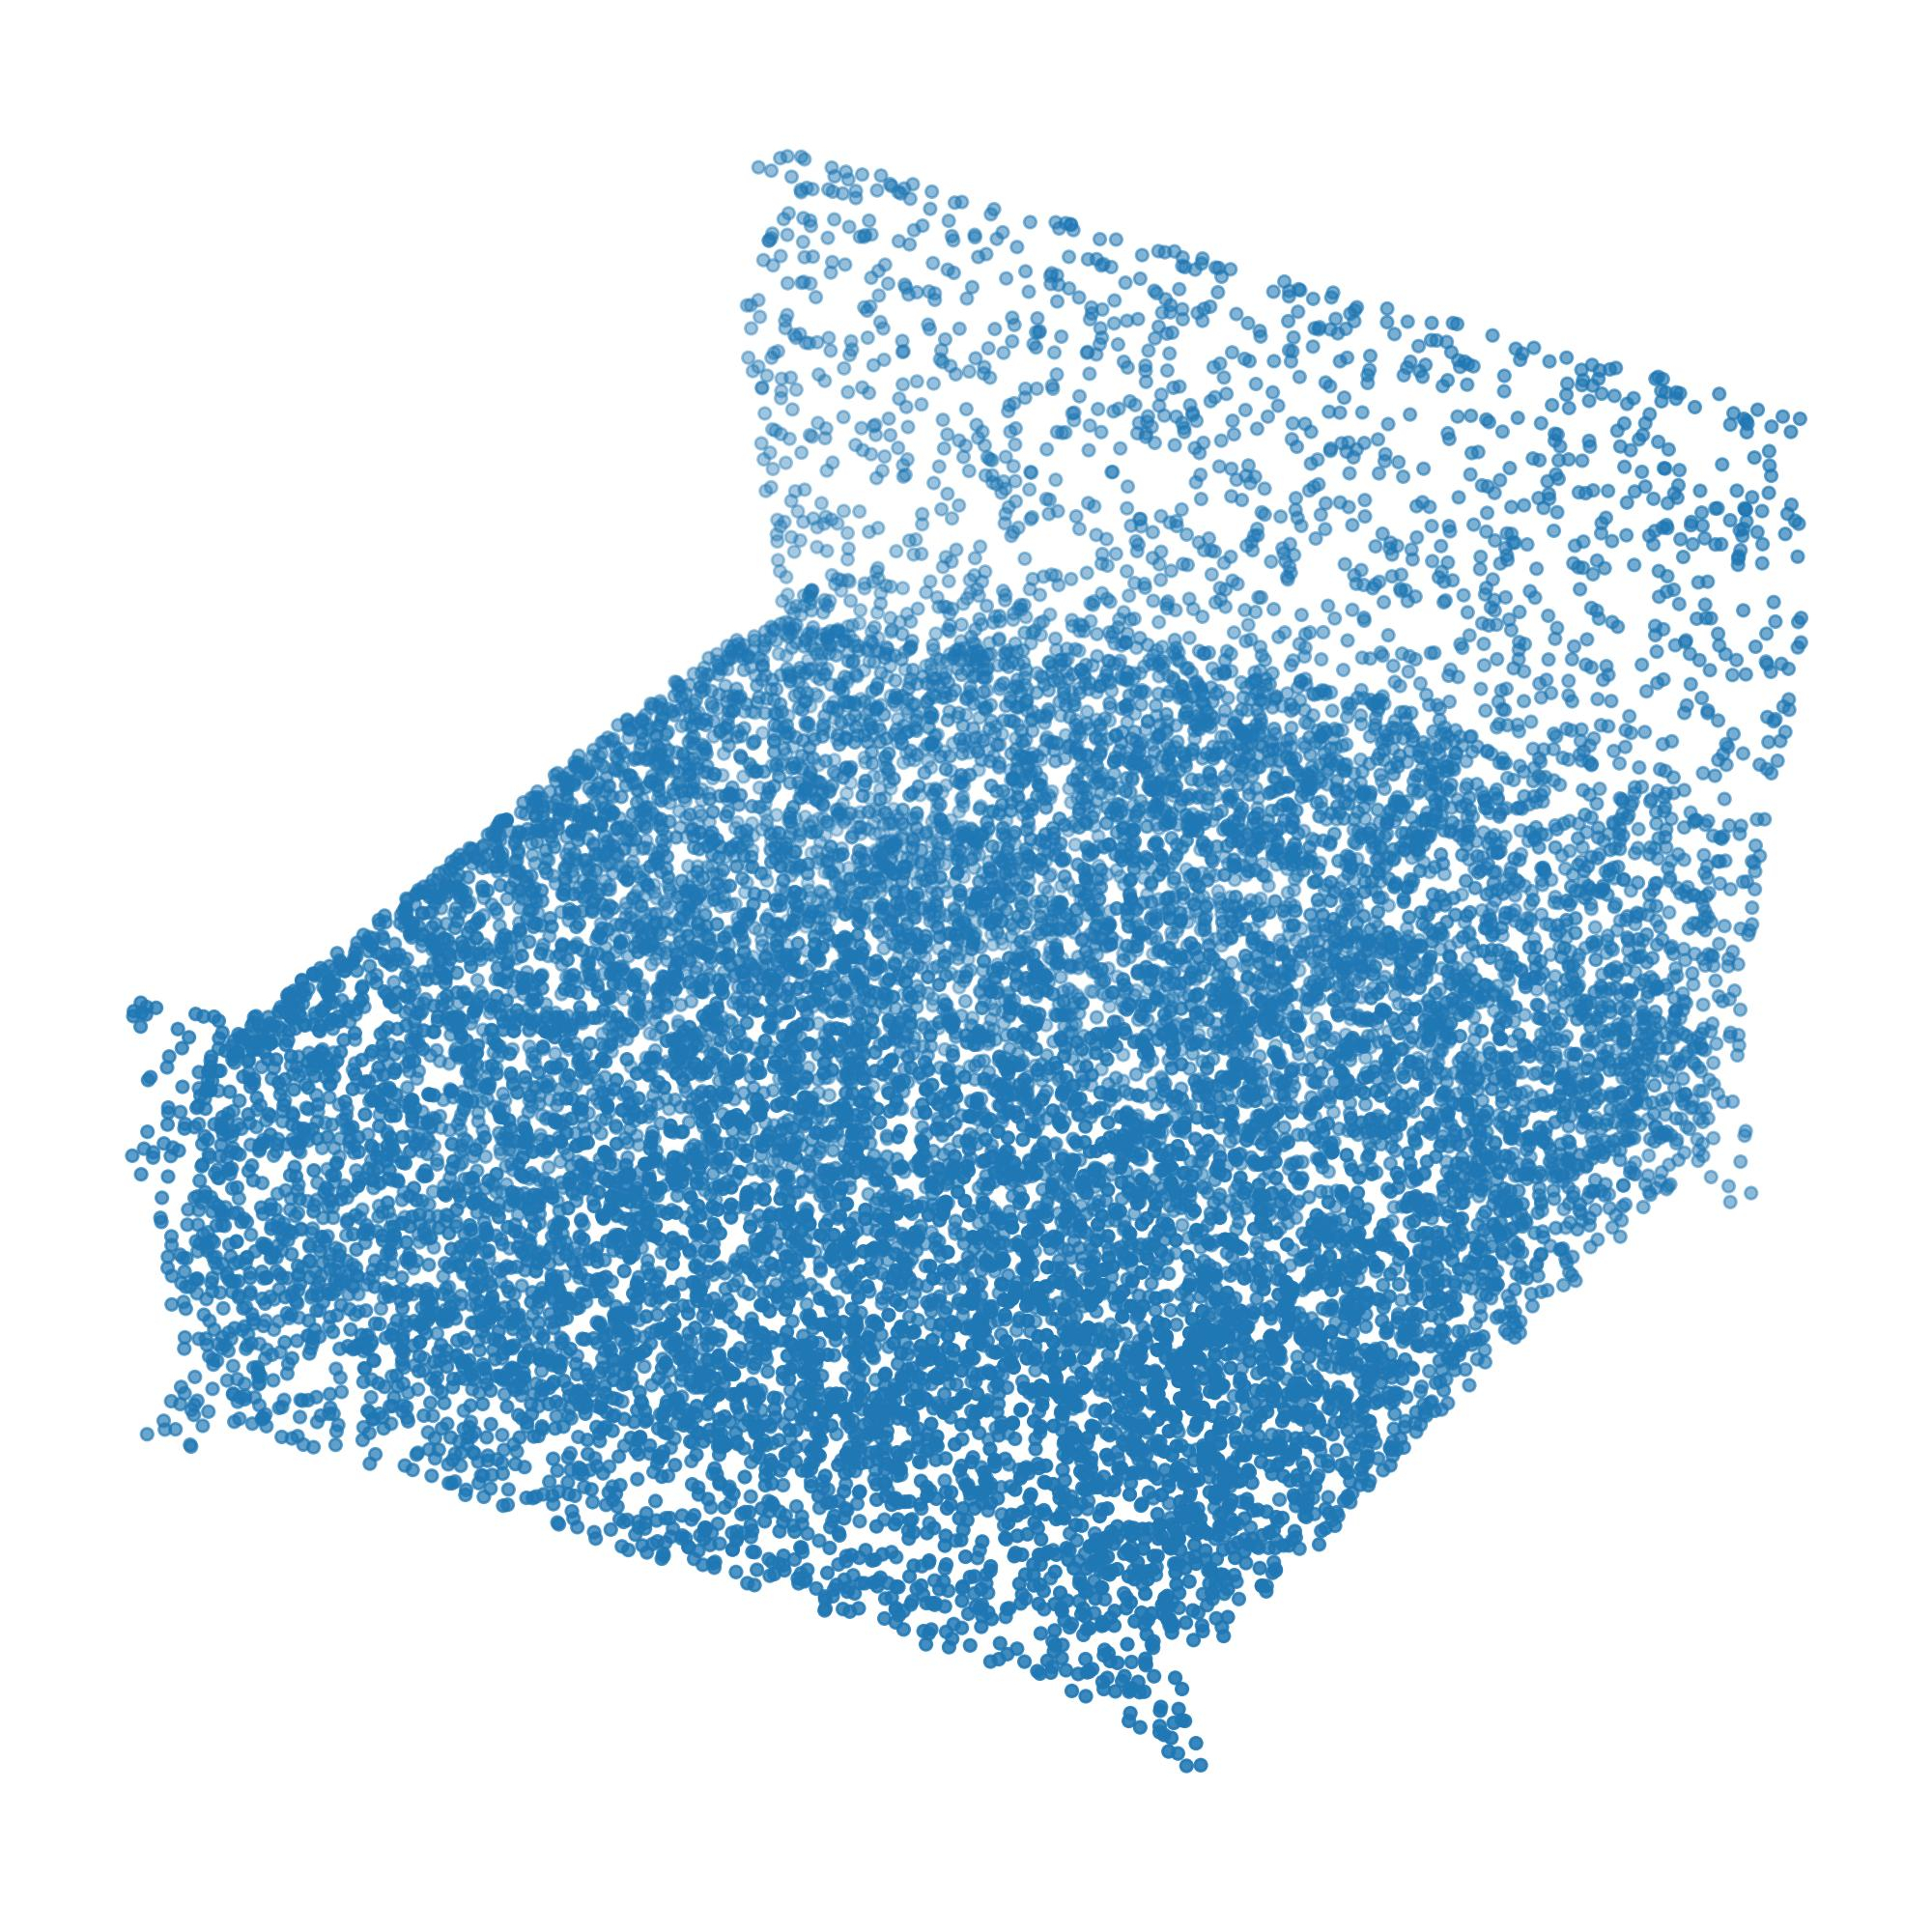
\includegraphics[scale=0.26]{imgs/example-mesh-pointcloud.jpg} }}
    \qquad
    \subfloat[\centering Renders obtained applying textures]{{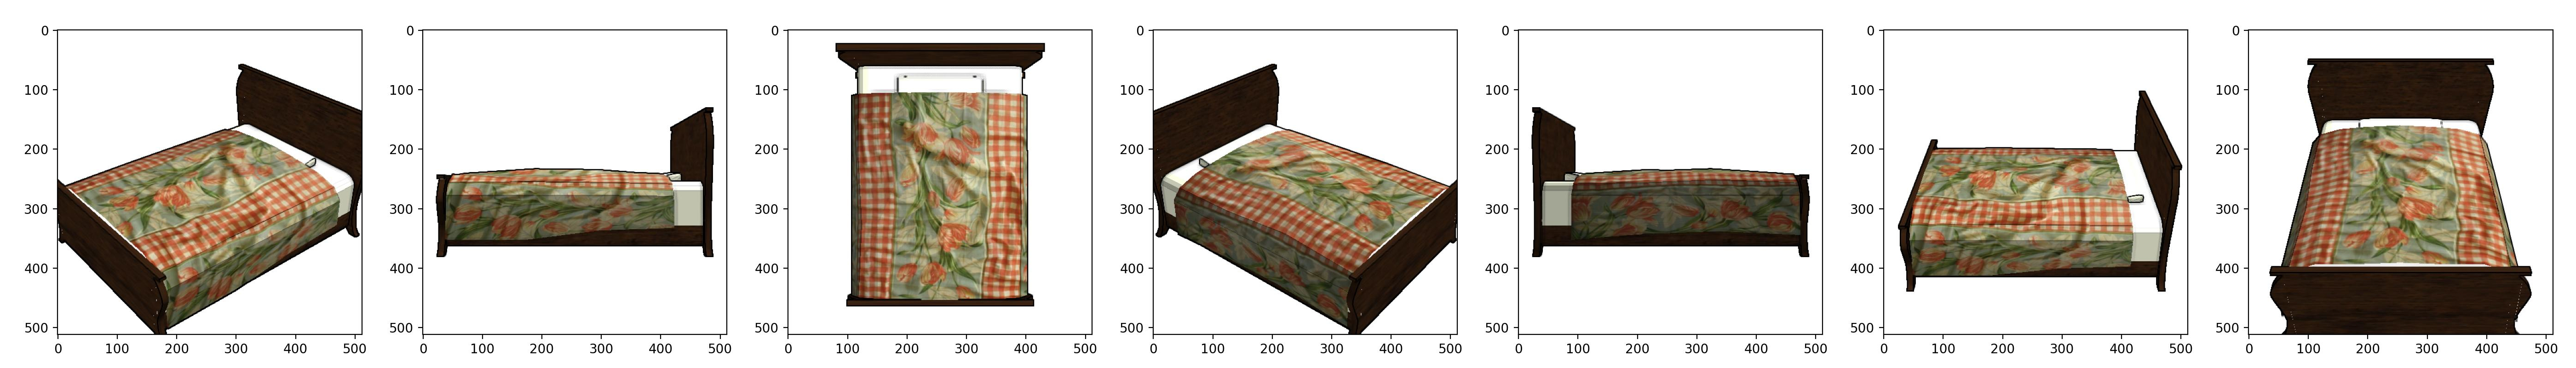
\includegraphics[scale=0.21]{imgs/example-mesh-renders.jpg} }}
    \caption{Random sample from the dataset}
\end{figure}
\subsection{The Dataset: ShapeNet}
ShapeNet\footnote{\url{https://shapenet.org}} is an ongoing effort to establish a richly-annotated, large-scale dataset of 3D shapes. We provide researchers around the world with this data to enable research in computer graphics, computer vision, robotics, and other related disciplines. ShapeNet is a collaborative effort between researchers at Princeton, Stanford and TTIC.
ShapeNet consists of several subsets:
\begin{itemize}
    \item \textbf{ShapeNetCore}: a subset of the full ShapeNet dataset with single clean 3D models and manually verified category and alignment annotations. It covers $55$ common object categories with about $51,300$ unique 3D models. The $12$ object categories of PASCAL 3D+, a popular computer vision 3D benchmark dataset, are all covered by ShapeNetCore.
    \item \textbf{ShapeNetSem} a smaller, more densely annotated subset consisting of $12,000$ models spread over a broader set of $270$ categories. In addition to manually verified category labels and consistent alignments, these models are annotated with real-world dimensions, estimates of their material composition at the category level, and estimates of their total volume and weight.
\end{itemize}
\textbf{The project was developed using ShapeNetSem for the following reasons:}
\begin{itemize}
    \item it includes pre-rendered screenshots of each model from 6 canonical orientations (front, back, left, right, bottom, top), and another 6 "turn table" positions around the model;
    \item the included \texttt{metadata.csv} file provides metadata with class labels associated with each model\footnote{Each model in ShapeNet is linked to an appropriate synset in WordNet: WordNet is a large lexical database of English. Nouns, verbs, adjectives and adverbs are grouped into sets of cognitive synonyms (synsets), each expressing a distinct concept (\url{https://wordnet.princeton.edu}).};
    \item each object is identified by means of a unique hexadecimal string\\(i.e. \texttt{100f39dce7690f59efb94709f30ce0d2});
\end{itemize}
Due to size limitations I did not provide the dataset included in the shared Google drive. To get access to it, I made a request using University of Pisa education email address. The following credentials can be used to \textbf{directly download} the dataset from the ShapeNet organization website\footnote{\url{https://shapenet.org}}:
\begin{lstlisting}[language=bash,frame=single]
Username: rambodrahmani
Password: Cnk4mBZ77Z5Av6v
\end{lstlisting}
Some preliminary preprocessing tasks were performed as detailed in the following subsections.
\subsection{Merge 3D models and renders}
In the original dataset, 3D models \texttt{.obj} files and rendered \texttt{.png} files are provided in separate \texttt{.zip} archives.
\begin{lstlisting}[language=bash]
$ tree ShapeNetSem-models
\end{lstlisting}
\dirtree{%
.1 ShapeNetSem-models.
.2 1004f30be305f33d28a1548e344f0e2e.mtl.
.2 1004f30be305f33d28a1548e344f0e2e.obj.
.2 100f39dce7690f59efb94709f30ce0d2.mtl.
.2 100f39dce7690f59efb94709f30ce0d2.obj.
.2 101354f9d8dede686f7b08d9de913afe.mtl.
.2 101354f9d8dede686f7b08d9de913afe.obj.
.2 ....
}
\begin{lstlisting}[language=bash]
$ tree ShapeNetSem-renders
\end{lstlisting}
\dirtree{%
.1 ShapeNetSem-models.
.2 1004f30be305f33d28a1548e344f0e2e.
.3 1004f30be305f33d28a1548e344f0e2e-0.png.
.3 1004f30be305f33d28a1548e344f0e2e-1.png.
.3 ....
.2 100f39dce7690f59efb94709f30ce0d2.
.3 100f39dce7690f59efb94709f30ce0d2-0.png.
.3 100f39dce7690f59efb94709f30ce0d2-1.png.
.3 ....
.2 ....
}
\noindent
The first preprocessing task consisted in merging this two archives to have all the raw data in a single directory. During this process, only \texttt{.obj} and \texttt{.png} files were maintained since \texttt{.mtl} files are of no use for our purposes. The resulting preliminary structure of the dataset is the following:
\begin{lstlisting}[language=bash]
$ tree ShapeNetSem-renders
\end{lstlisting}
\dirtree{%
.1 ShapeNetSem-models.
.2 1004f30be305f33d28a1548e344f0e2e.
.3 1004f30be305f33d28a1548e344f0e2e.obj.
.3 1004f30be305f33d28a1548e344f0e2e-0.png.
.3 1004f30be305f33d28a1548e344f0e2e-1.png.
.3 ....
.2 100f39dce7690f59efb94709f30ce0d2.
.3 100f39dce7690f59efb94709f30ce0d2.obj.
.3 100f39dce7690f59efb94709f30ce0d2-0.png.
.3 100f39dce7690f59efb94709f30ce0d2-1.png.
.3 ....
.2 ....
}
\noindent
\subsection{Organize data in macro-categories}
In the original dataset, models are divided in $270$ categories. I decided to aggregate them in $20$ macro-categories in order to:
\begin{itemize}
    \item have a higher number of samples for each category;
    \item make the classification task more comprehensible;
\end{itemize}
In order to achieve this result, the \texttt{metadata.csv} file was used.
\begin{figure}[H]
    \centering
    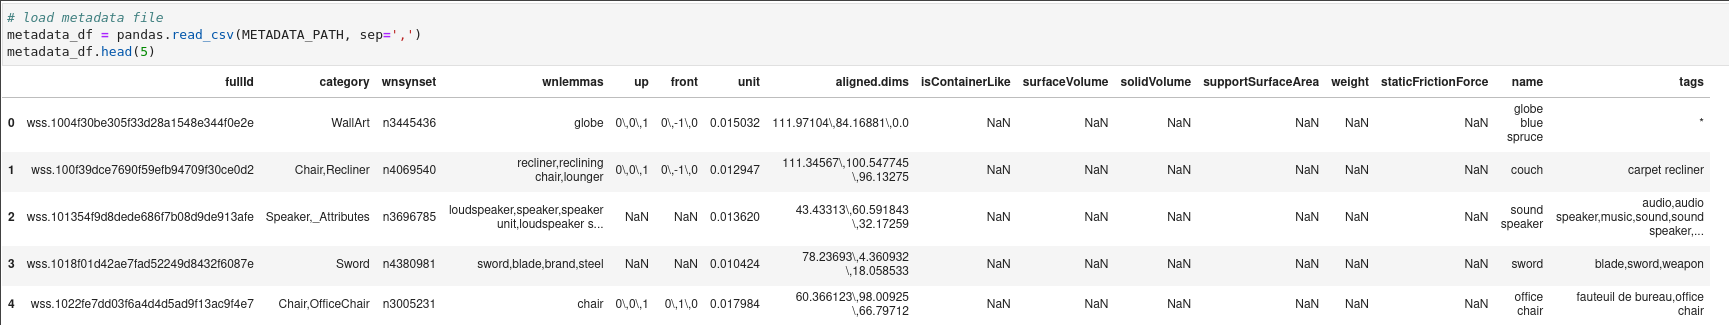
\includegraphics[scale=0.24]{imgs/metadata-pandas-df.png}
    \caption{Metadata \texttt{.csv} file loaded as \texttt{pandas} dataframe}
\end{figure}
\noindent
It provides the following information for each of the models:
\begin{itemize}
    \item \textbf{ID:} hexadecimal string used to uniquely identify each model in the ShapeNet dataset;
    \item \textbf{category:} object class label;
    \item \textbf{wnsynset:} identifies the associated synset in WordNet; the synset is a set of one or more synonyms that are interchangeable in some context without changing the truth value of the proposition in which they are embedded;
    \item \textbf{wnlemmas:} one or more lemmas associated to the given synset ID in WordNet; a lemma represents a specific sense of a specific word;
    \item \textbf{name:} object name;
    \item \textbf{tags:} additional tags associated with the object class label;
\end{itemize}
The following snippet extract from \texttt{metadata.csv} clarifies it better with examples:\\
\\
\setlength\extrarowheight{5pt}
\rowcolors{2}{gray!25}{white}
\begin{tabular}{|p{2cm}|p{2cm}|p{3.2cm}|p{2cm}|p{3.2cm}|p{3cm}}
\rowcolor{gray!50}
\hline
category & wnsynset & wnlemmas & name & tags\\
\hline
Chair, Recliner & n4069540 & recliner, reclining chair, lounger & couch & carpet recliner\\
\hline
Chair, OfficeChair & n3005231 & chair & office chair & fauteuil de bureau, office chair\\
\hline
Computer, Desktop & n3184677 & desktop computer & alienware & computer case pc\\
\hline
Plant & n17402 & plant, flora, plant, life & rose & flower, nature, petal, red, rose\\
\hline
\end{tabular}\\
\\
The possible values of the \texttt{category} field were reduced from $270$ to $20$ relaying on the information provided by other columns such as \texttt{wnsynset}, \texttt{wnlemmas}, \texttt{name} and \texttt{tags}.\\
\\
To conclude, putting it all together, for each object in the dataset we have the following information:
\begin{figure}[H]
    \centering
    \subfloat[\centering 3D Object]{{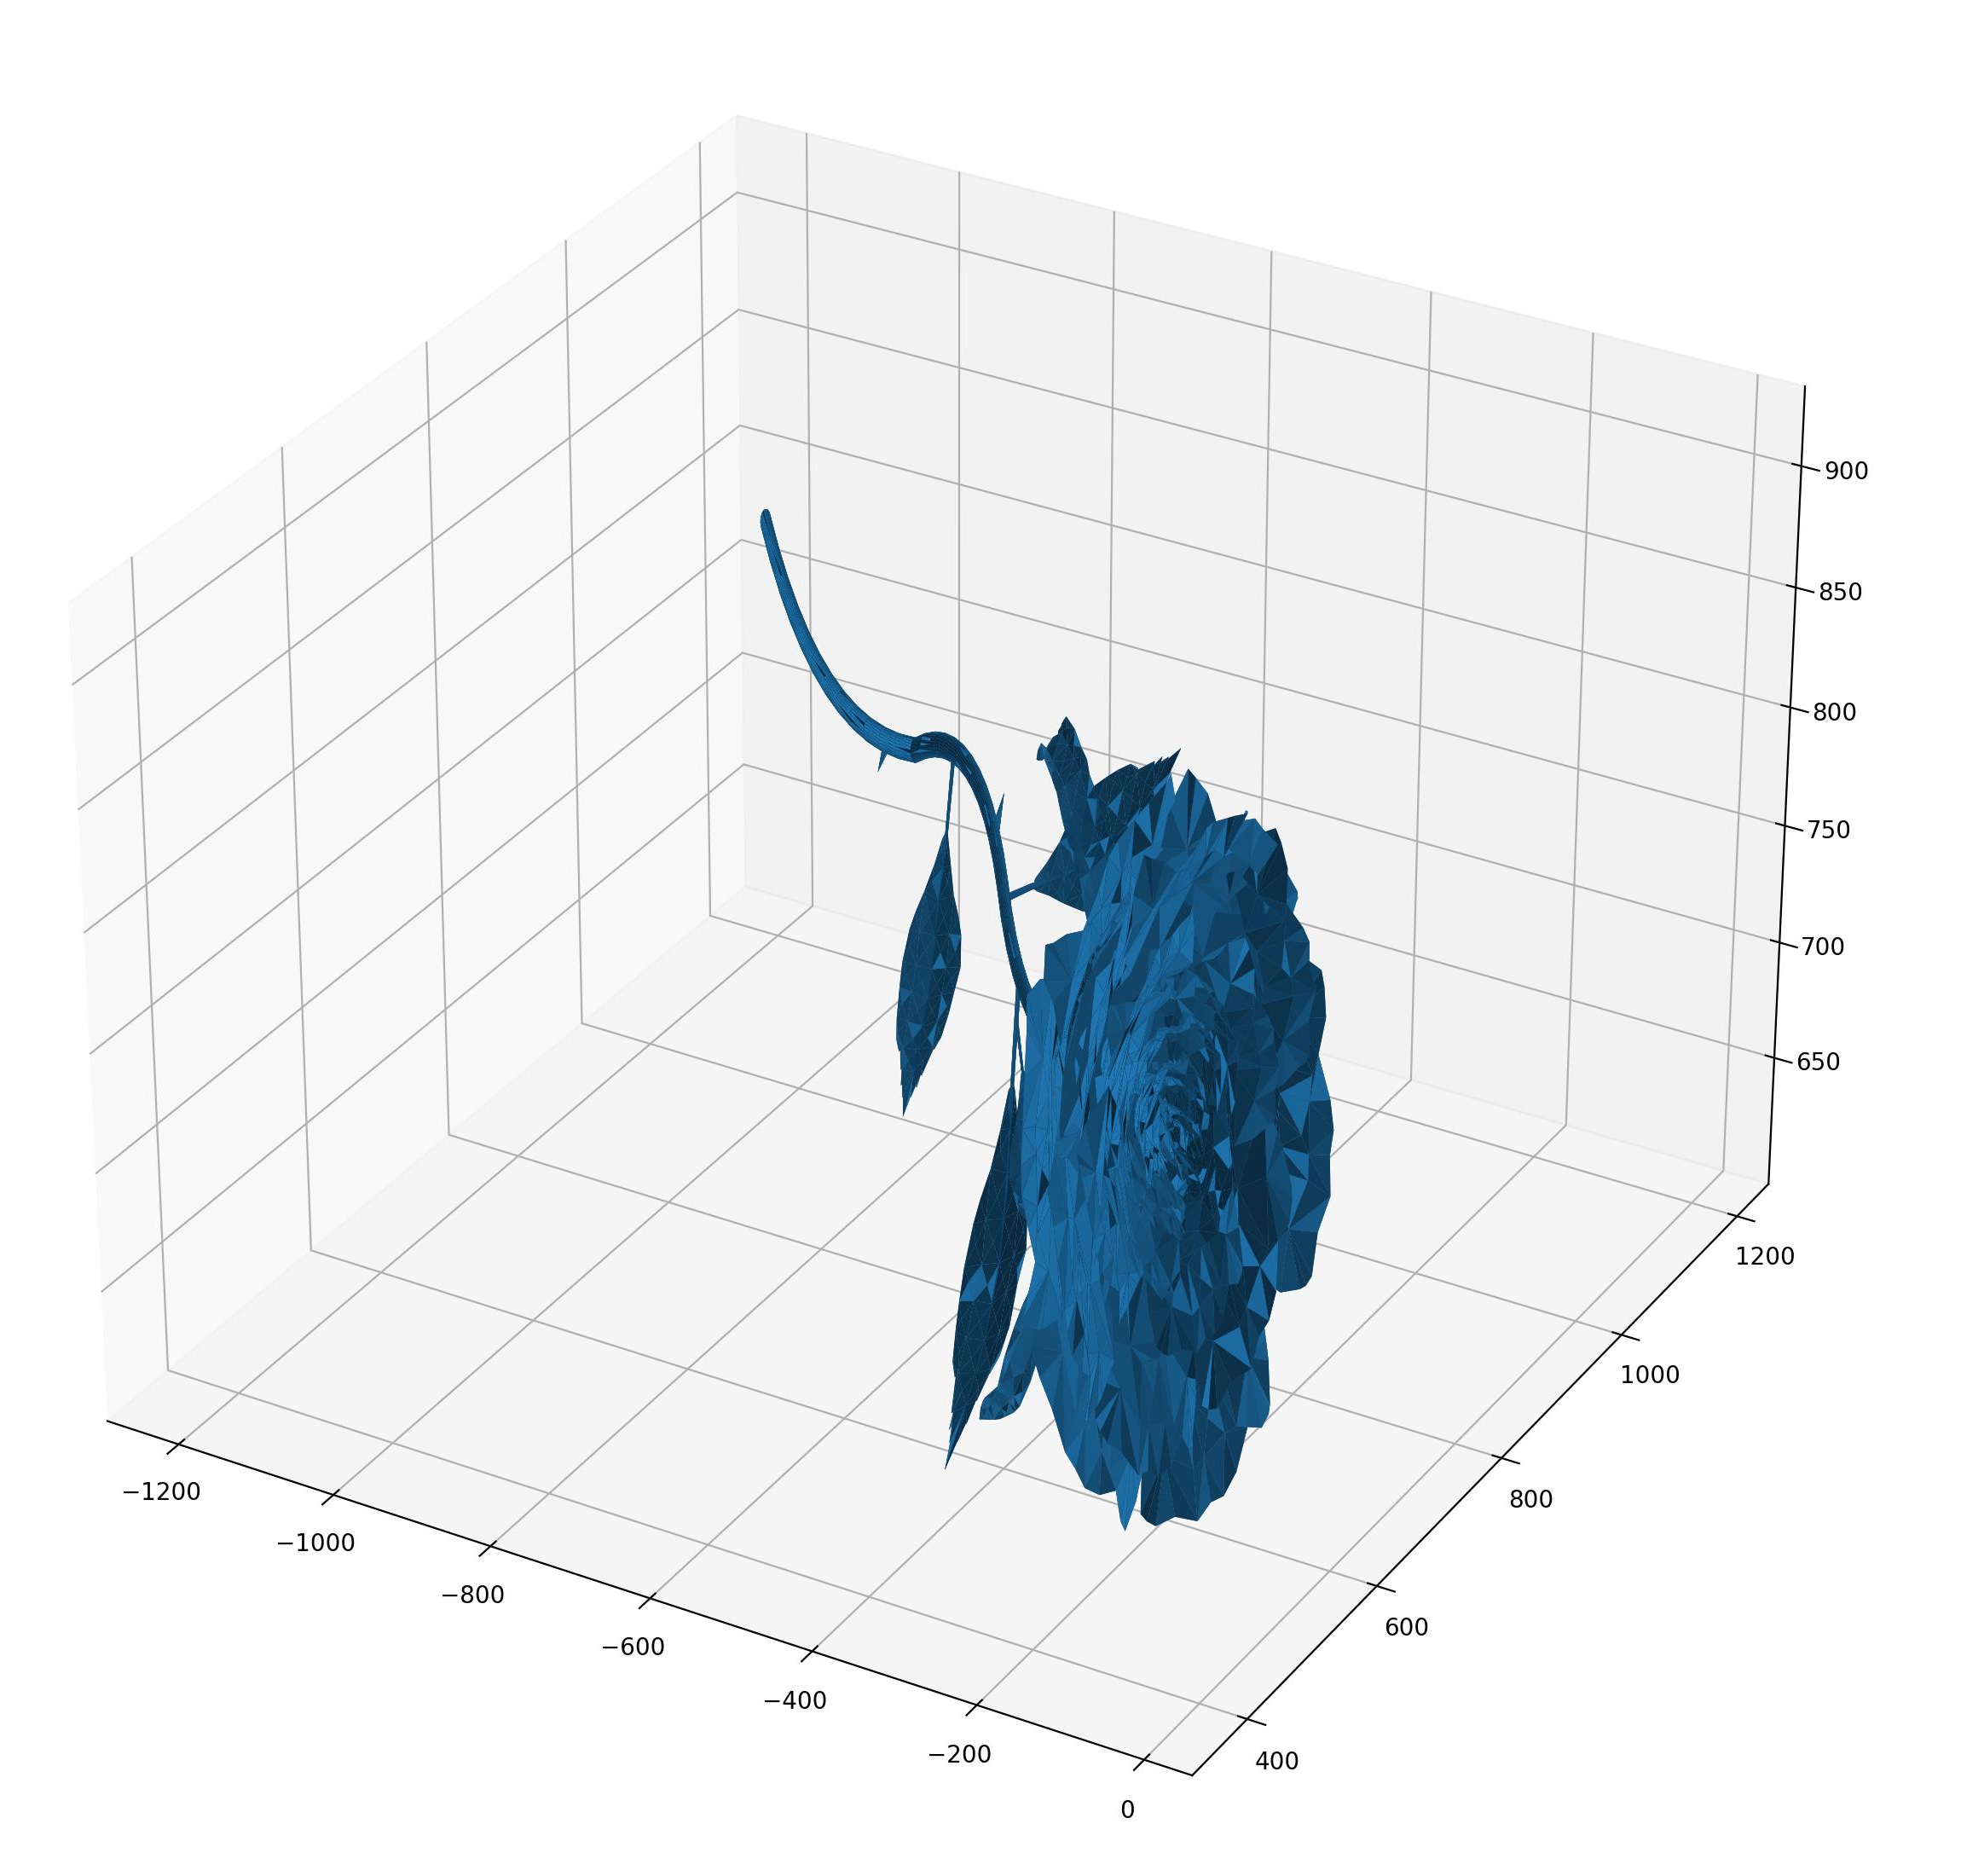
\includegraphics[scale=0.30]{imgs/example-mesh-2-trisurf.jpg} }}
    \qquad
    \subfloat[\centering Sampled Point Cloud]{{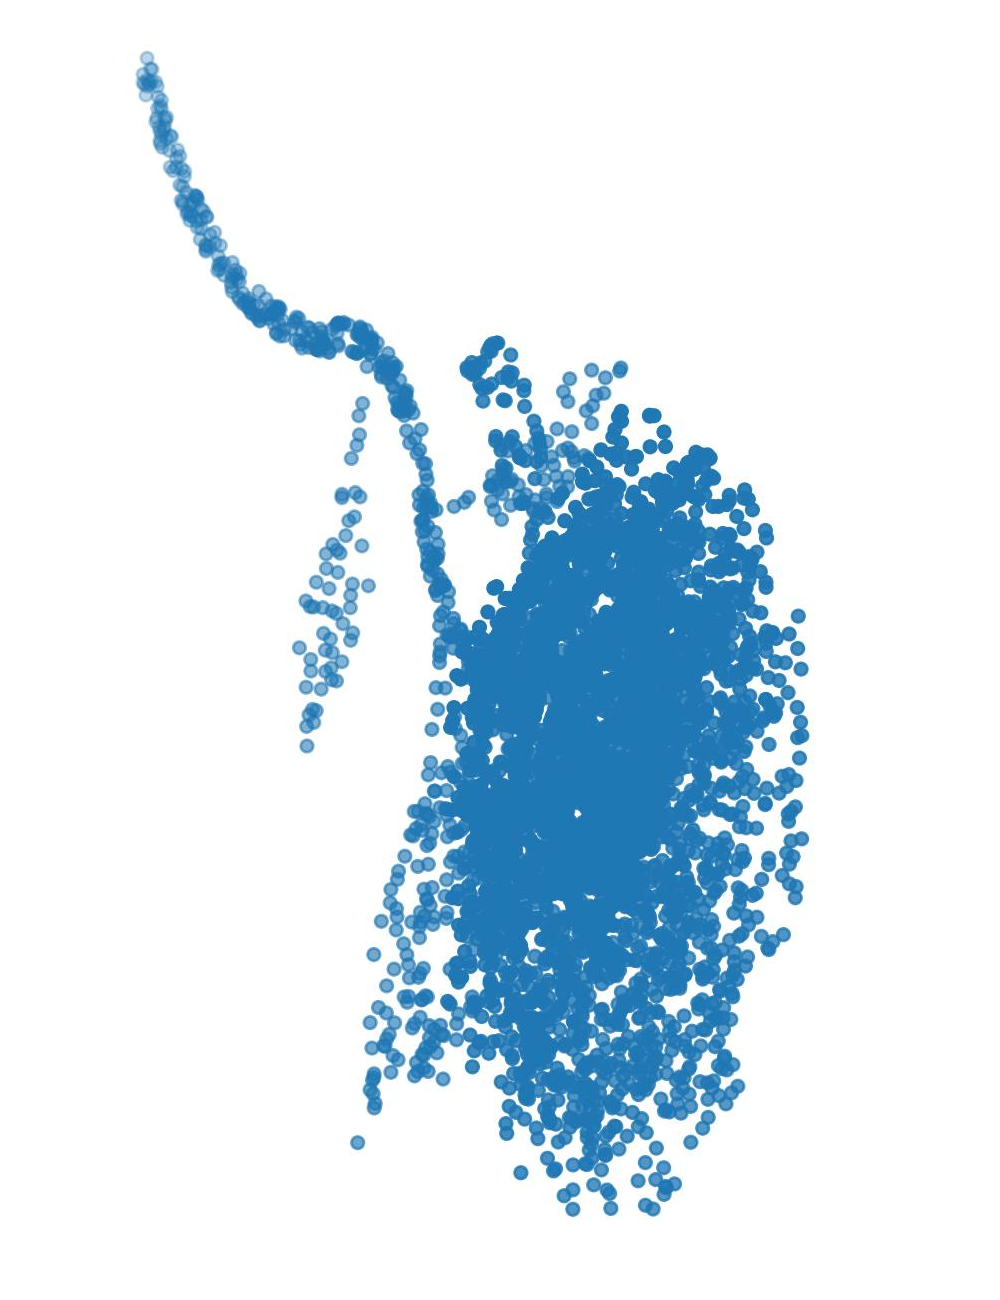
\includegraphics[scale=0.40]{imgs/example-mesh-2-pointcloud.jpg} }}
\end{figure}
\begin{figure}[H]
    \centering
    \subfloat[\centering Renders obtained applying textures]{{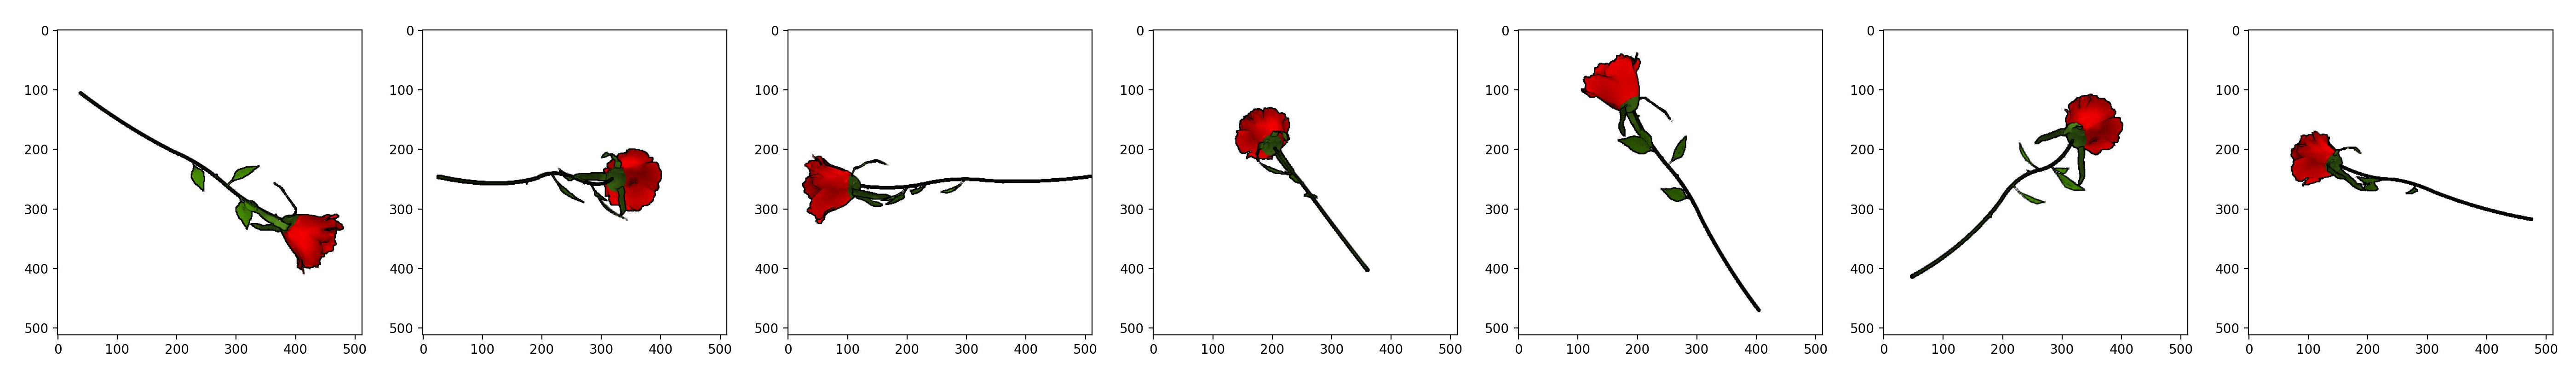
\includegraphics[scale=0.21]{imgs/example-mesh-2-renders.jpg} }}
\end{figure}
\begin{lstlisting}[language=bash,frame=single,caption={Random sample from the dataset},captionpos=b]
FullID: wss.1043b403dd2e79128081f4adb71040
Category: Plant
WNsynset: n17402
WNlemmas: plant, flora, plant life
Name: rose
Tags: boy, flower, girl, landscape, love, nature, petal, plant, red
\end{lstlisting}
After aggregating the initial $270$ categories, the following macro-categories were identified:
\begin{figure}[H]
    \centering
    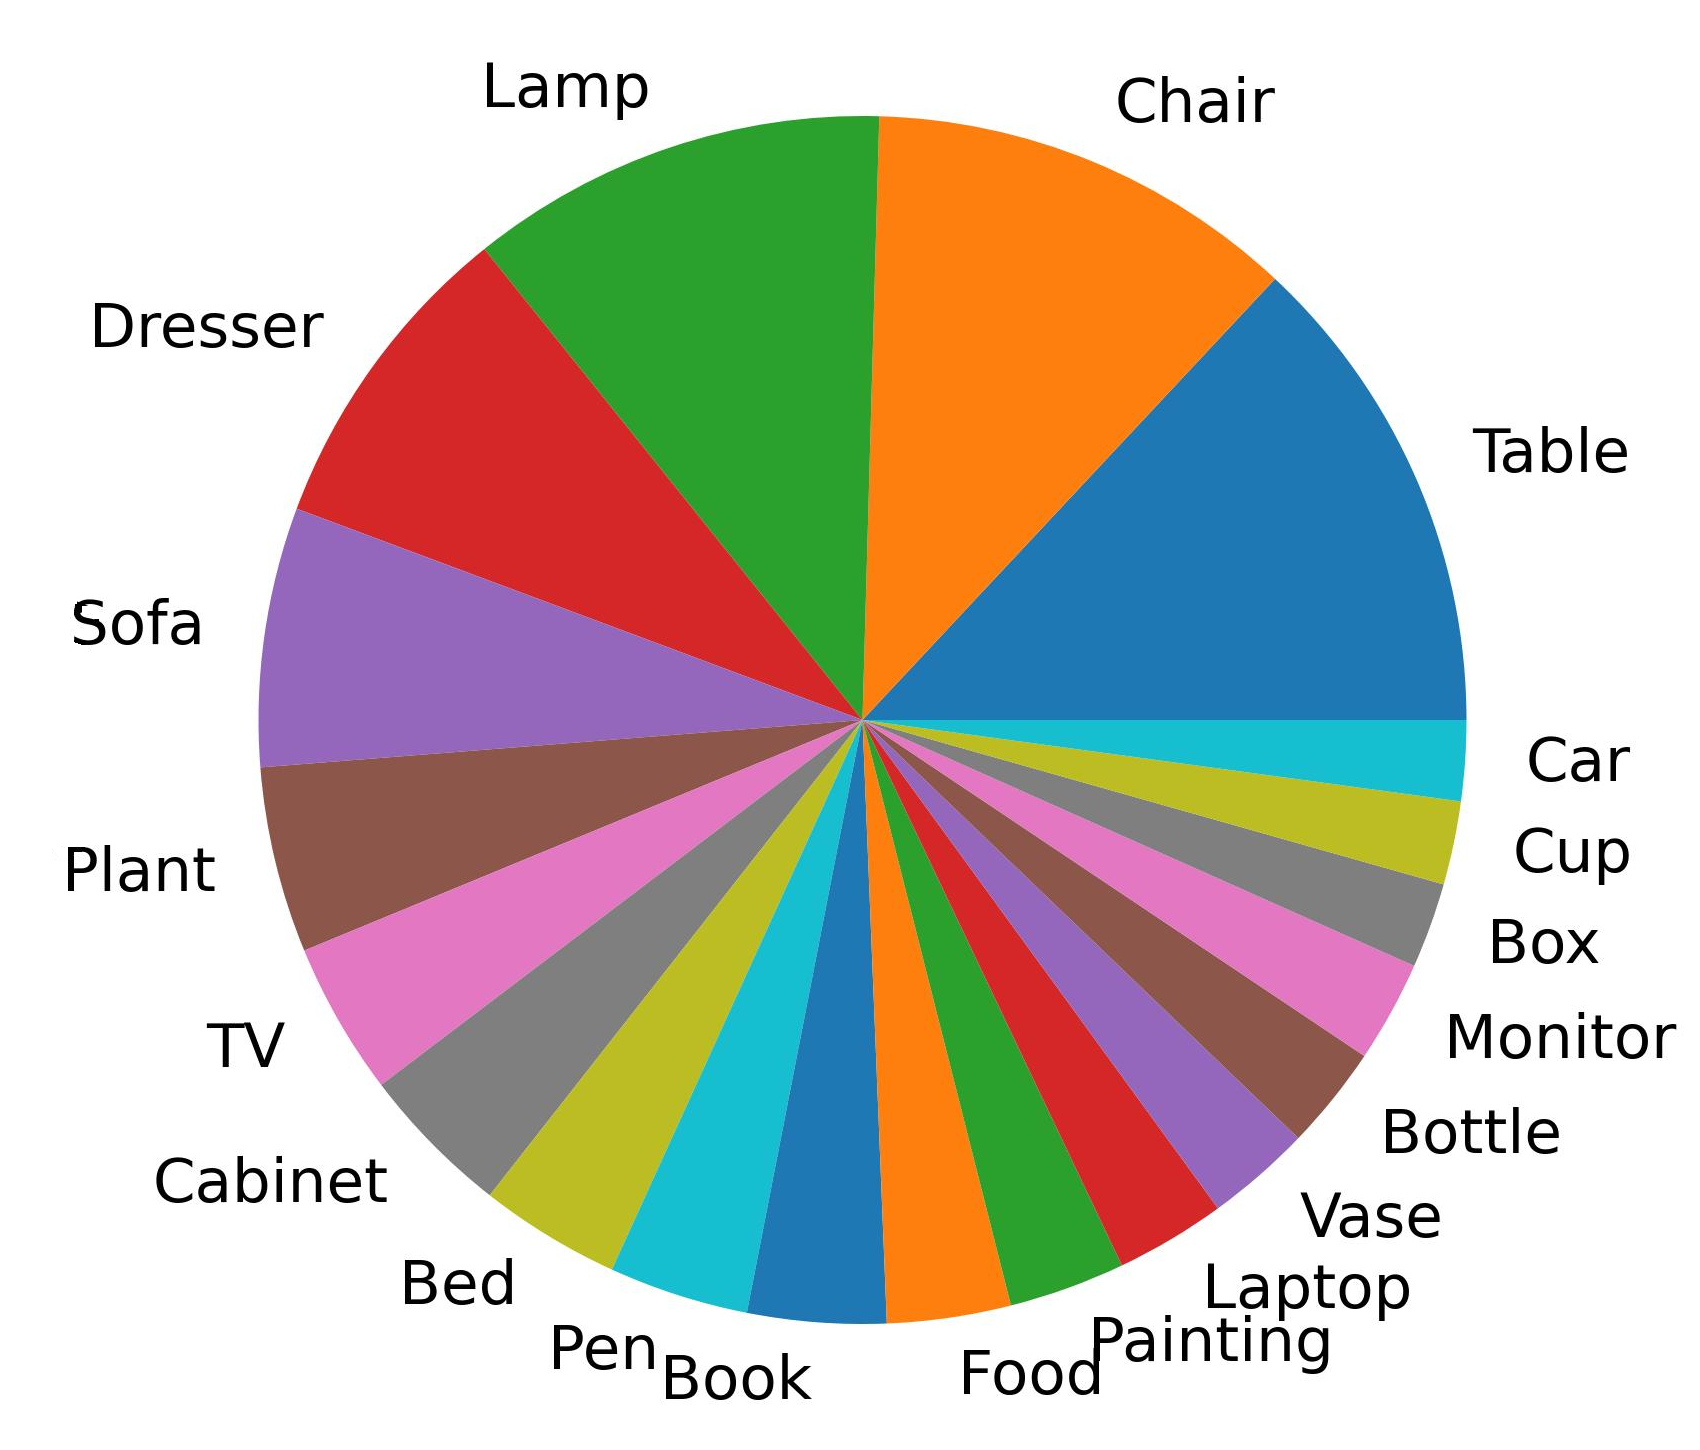
\includegraphics[scale=0.50]{imgs/macro-categories.jpg}
    \caption{Macro-categories}
\end{figure}
\subsection{Dataset balancing}
Imbalanced classifications pose a challenge for predictive modeling as most of the machine learning algorithms used for classification were designed around the assumption of an equal number of examples for each class. This results in models that have poor predictive performance, specifically for the minority class. Even if in the case under analysis there is no single minority class with higher importance, like it happens in medical applications, it is still important to balance the samples for each class.\\
\\
As it can be seen from the following bar charts, the dataset is not balanced. In addition, the quantity of images samples is higher than the one of 3D point clouds; this is understandable since for each 3D model 12 pre-rendered screenshots are provided.
\begin{figure}[H]
    \centering
    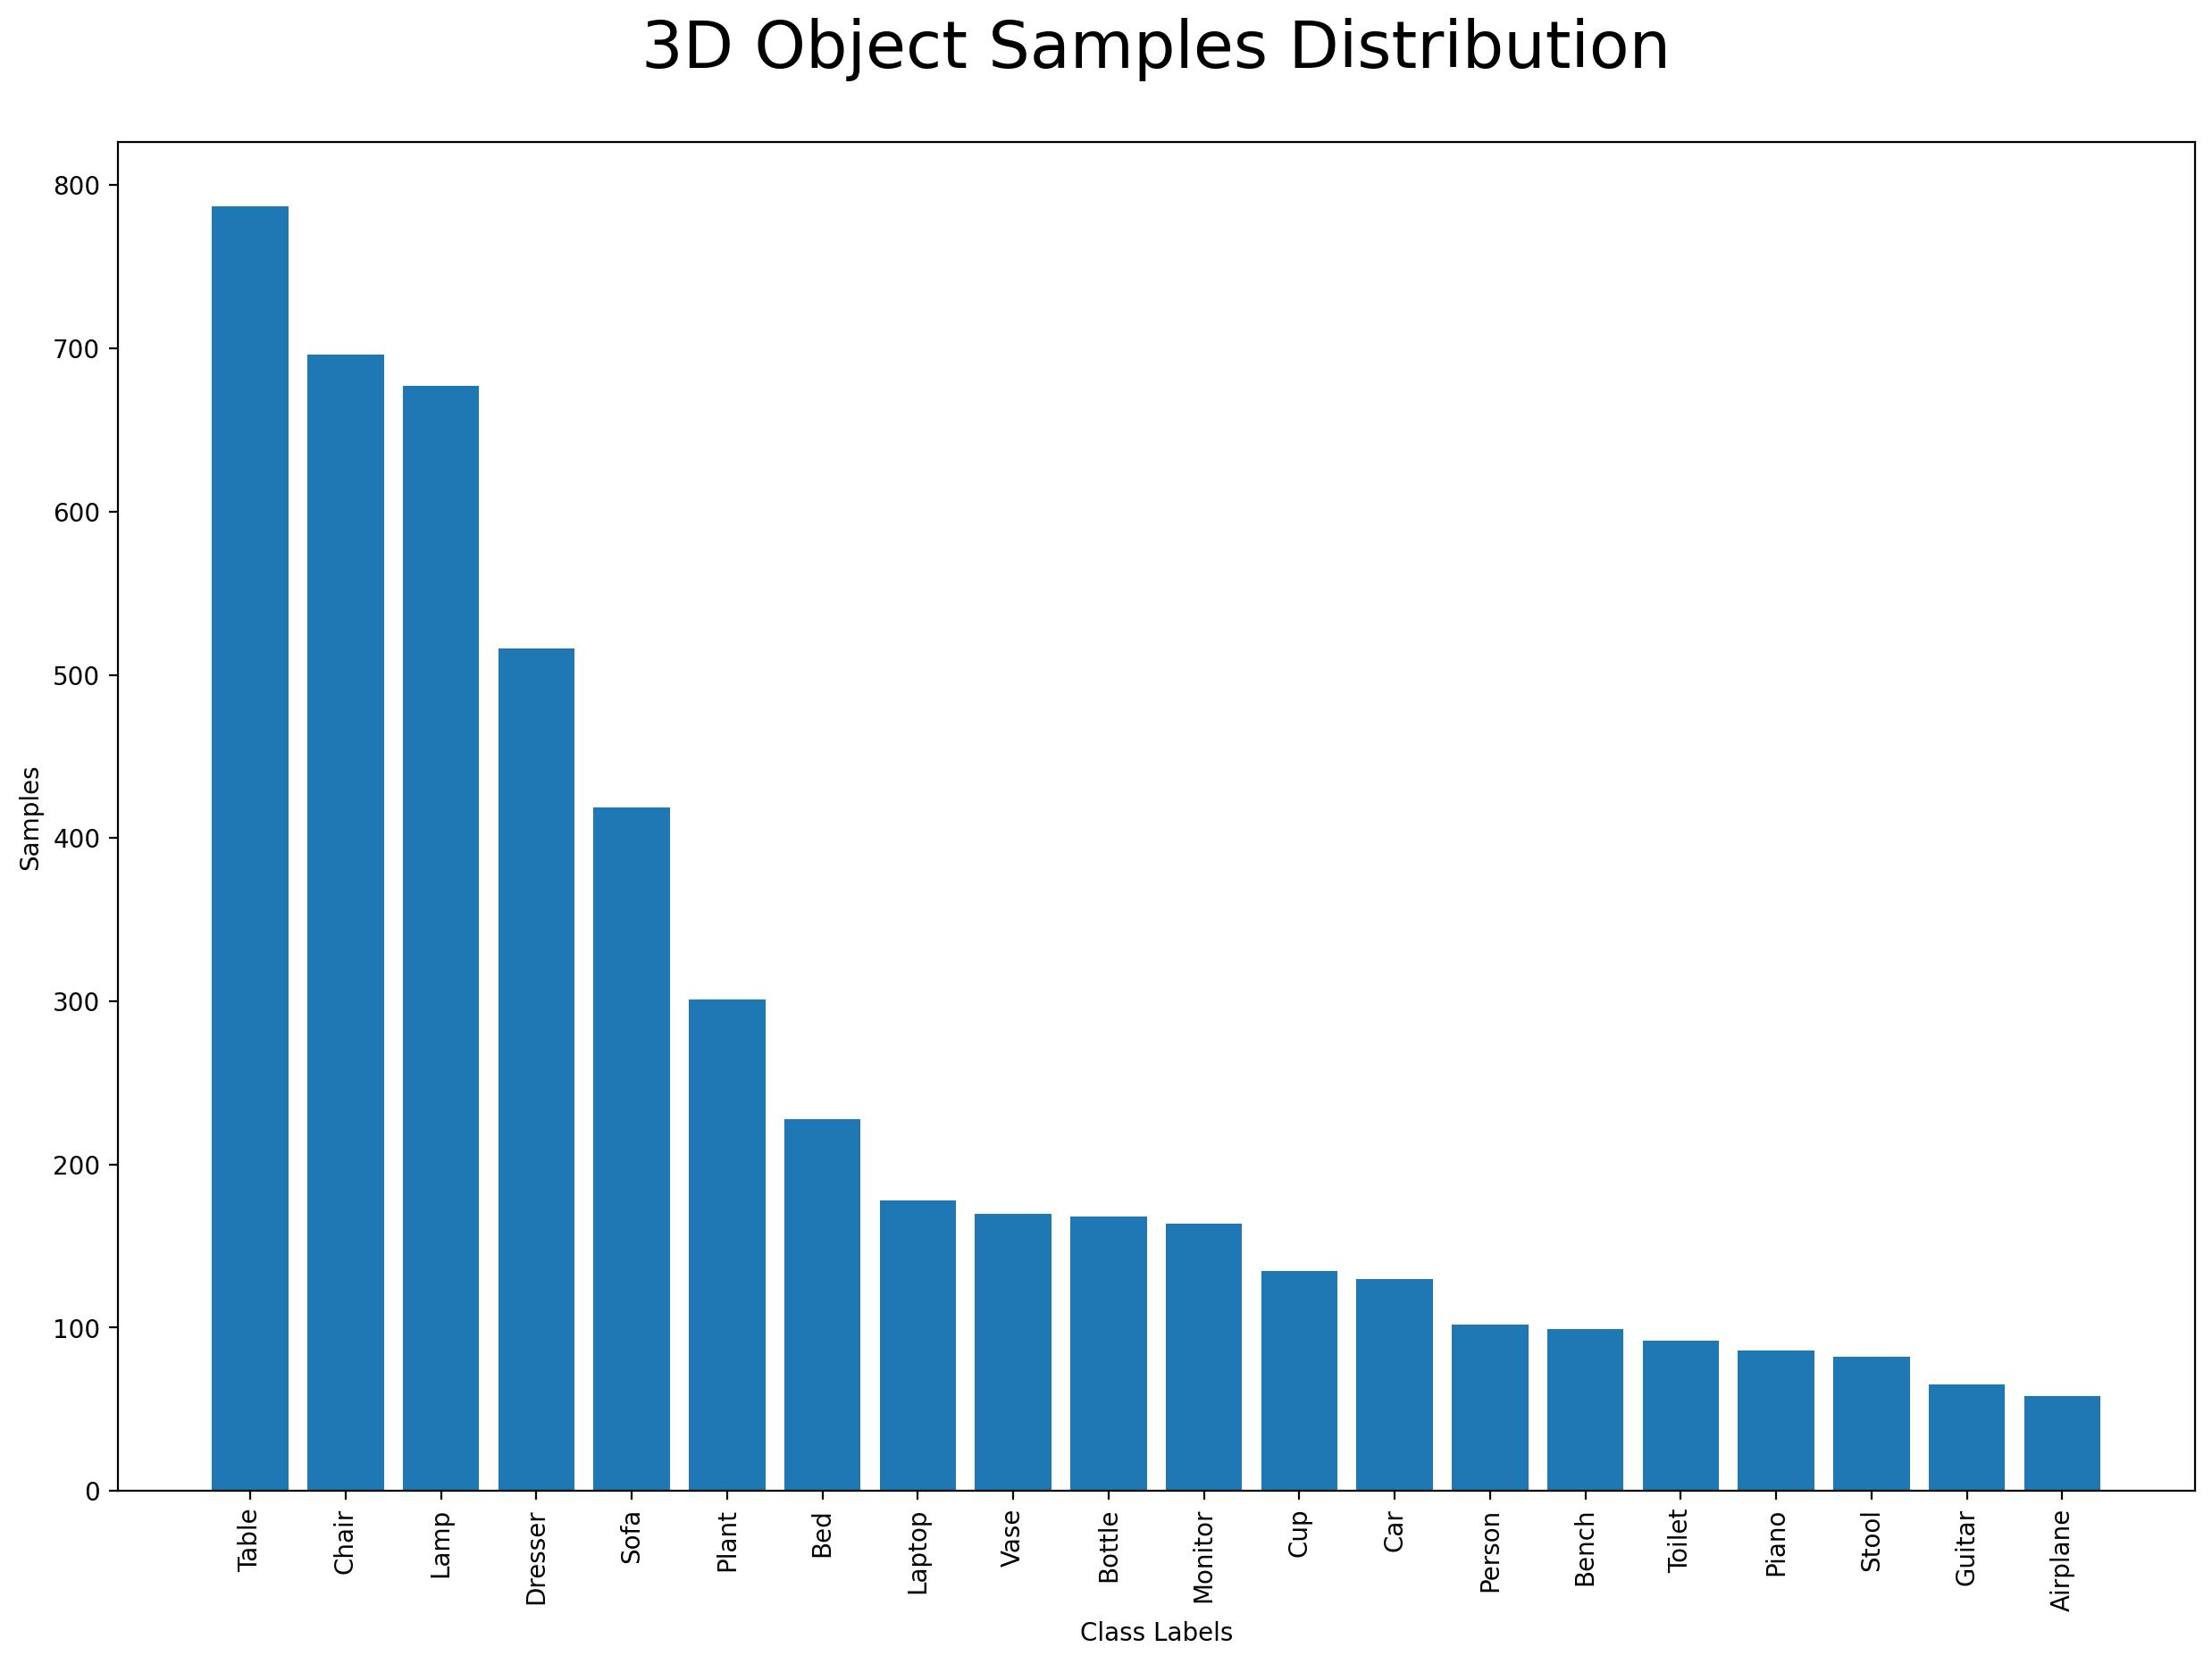
\includegraphics[scale=0.35]{imgs/3d-object-samples-distribution.jpg}
    \caption{3D Object Samples per class}
\end{figure}
\begin{figure}[H]
    \centering
    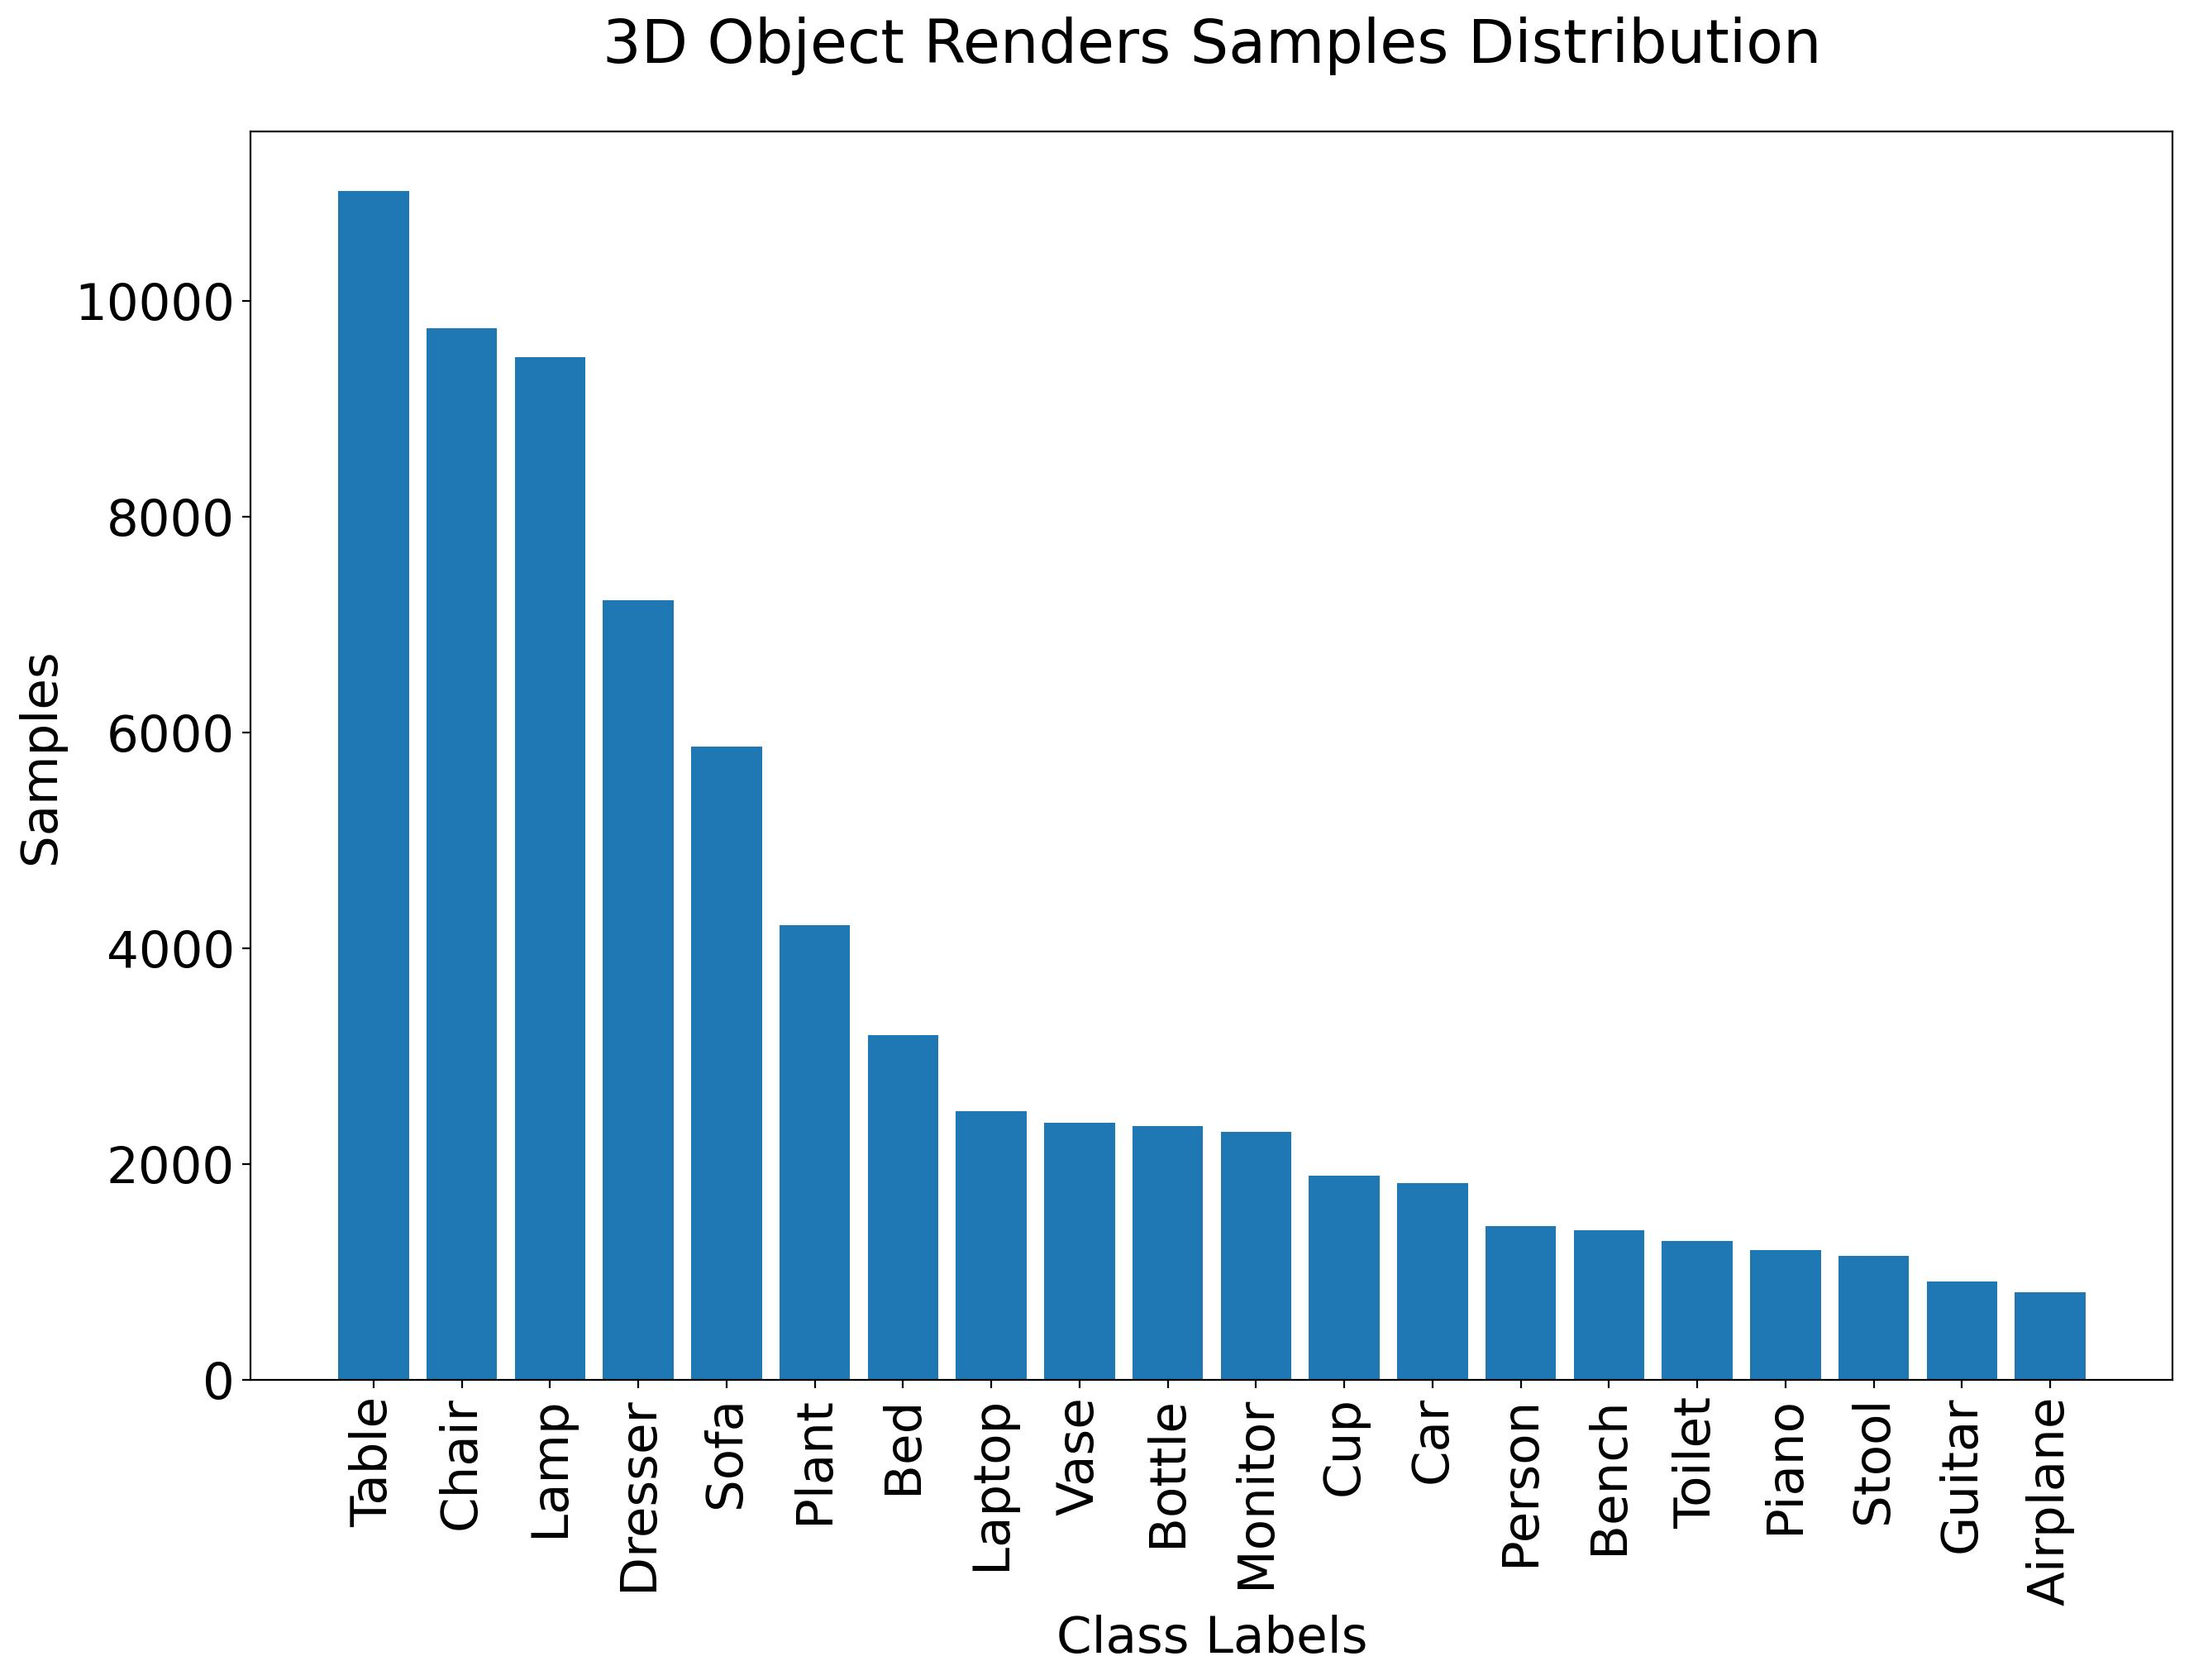
\includegraphics[scale=0.35]{imgs/3d-object-renders-samples-distribution.jpg}
    \caption{RGB Images (3D Objects Renders) Samples per class}
\end{figure}
\noindent
In this case, undersampling was not an option since this would mean loosing almost $85\%$ of the samples of the majority class. Instead, the choice was made to use \textbf{oversampling}. The ModelNet \cite{wu20153d} dataset\footnote{\url{https://modelnet.cs.princeton.edu/}} was used to augment 3D objects. After oversampling, this is the final result obtained:
\begin{figure}[H]
    \centering
    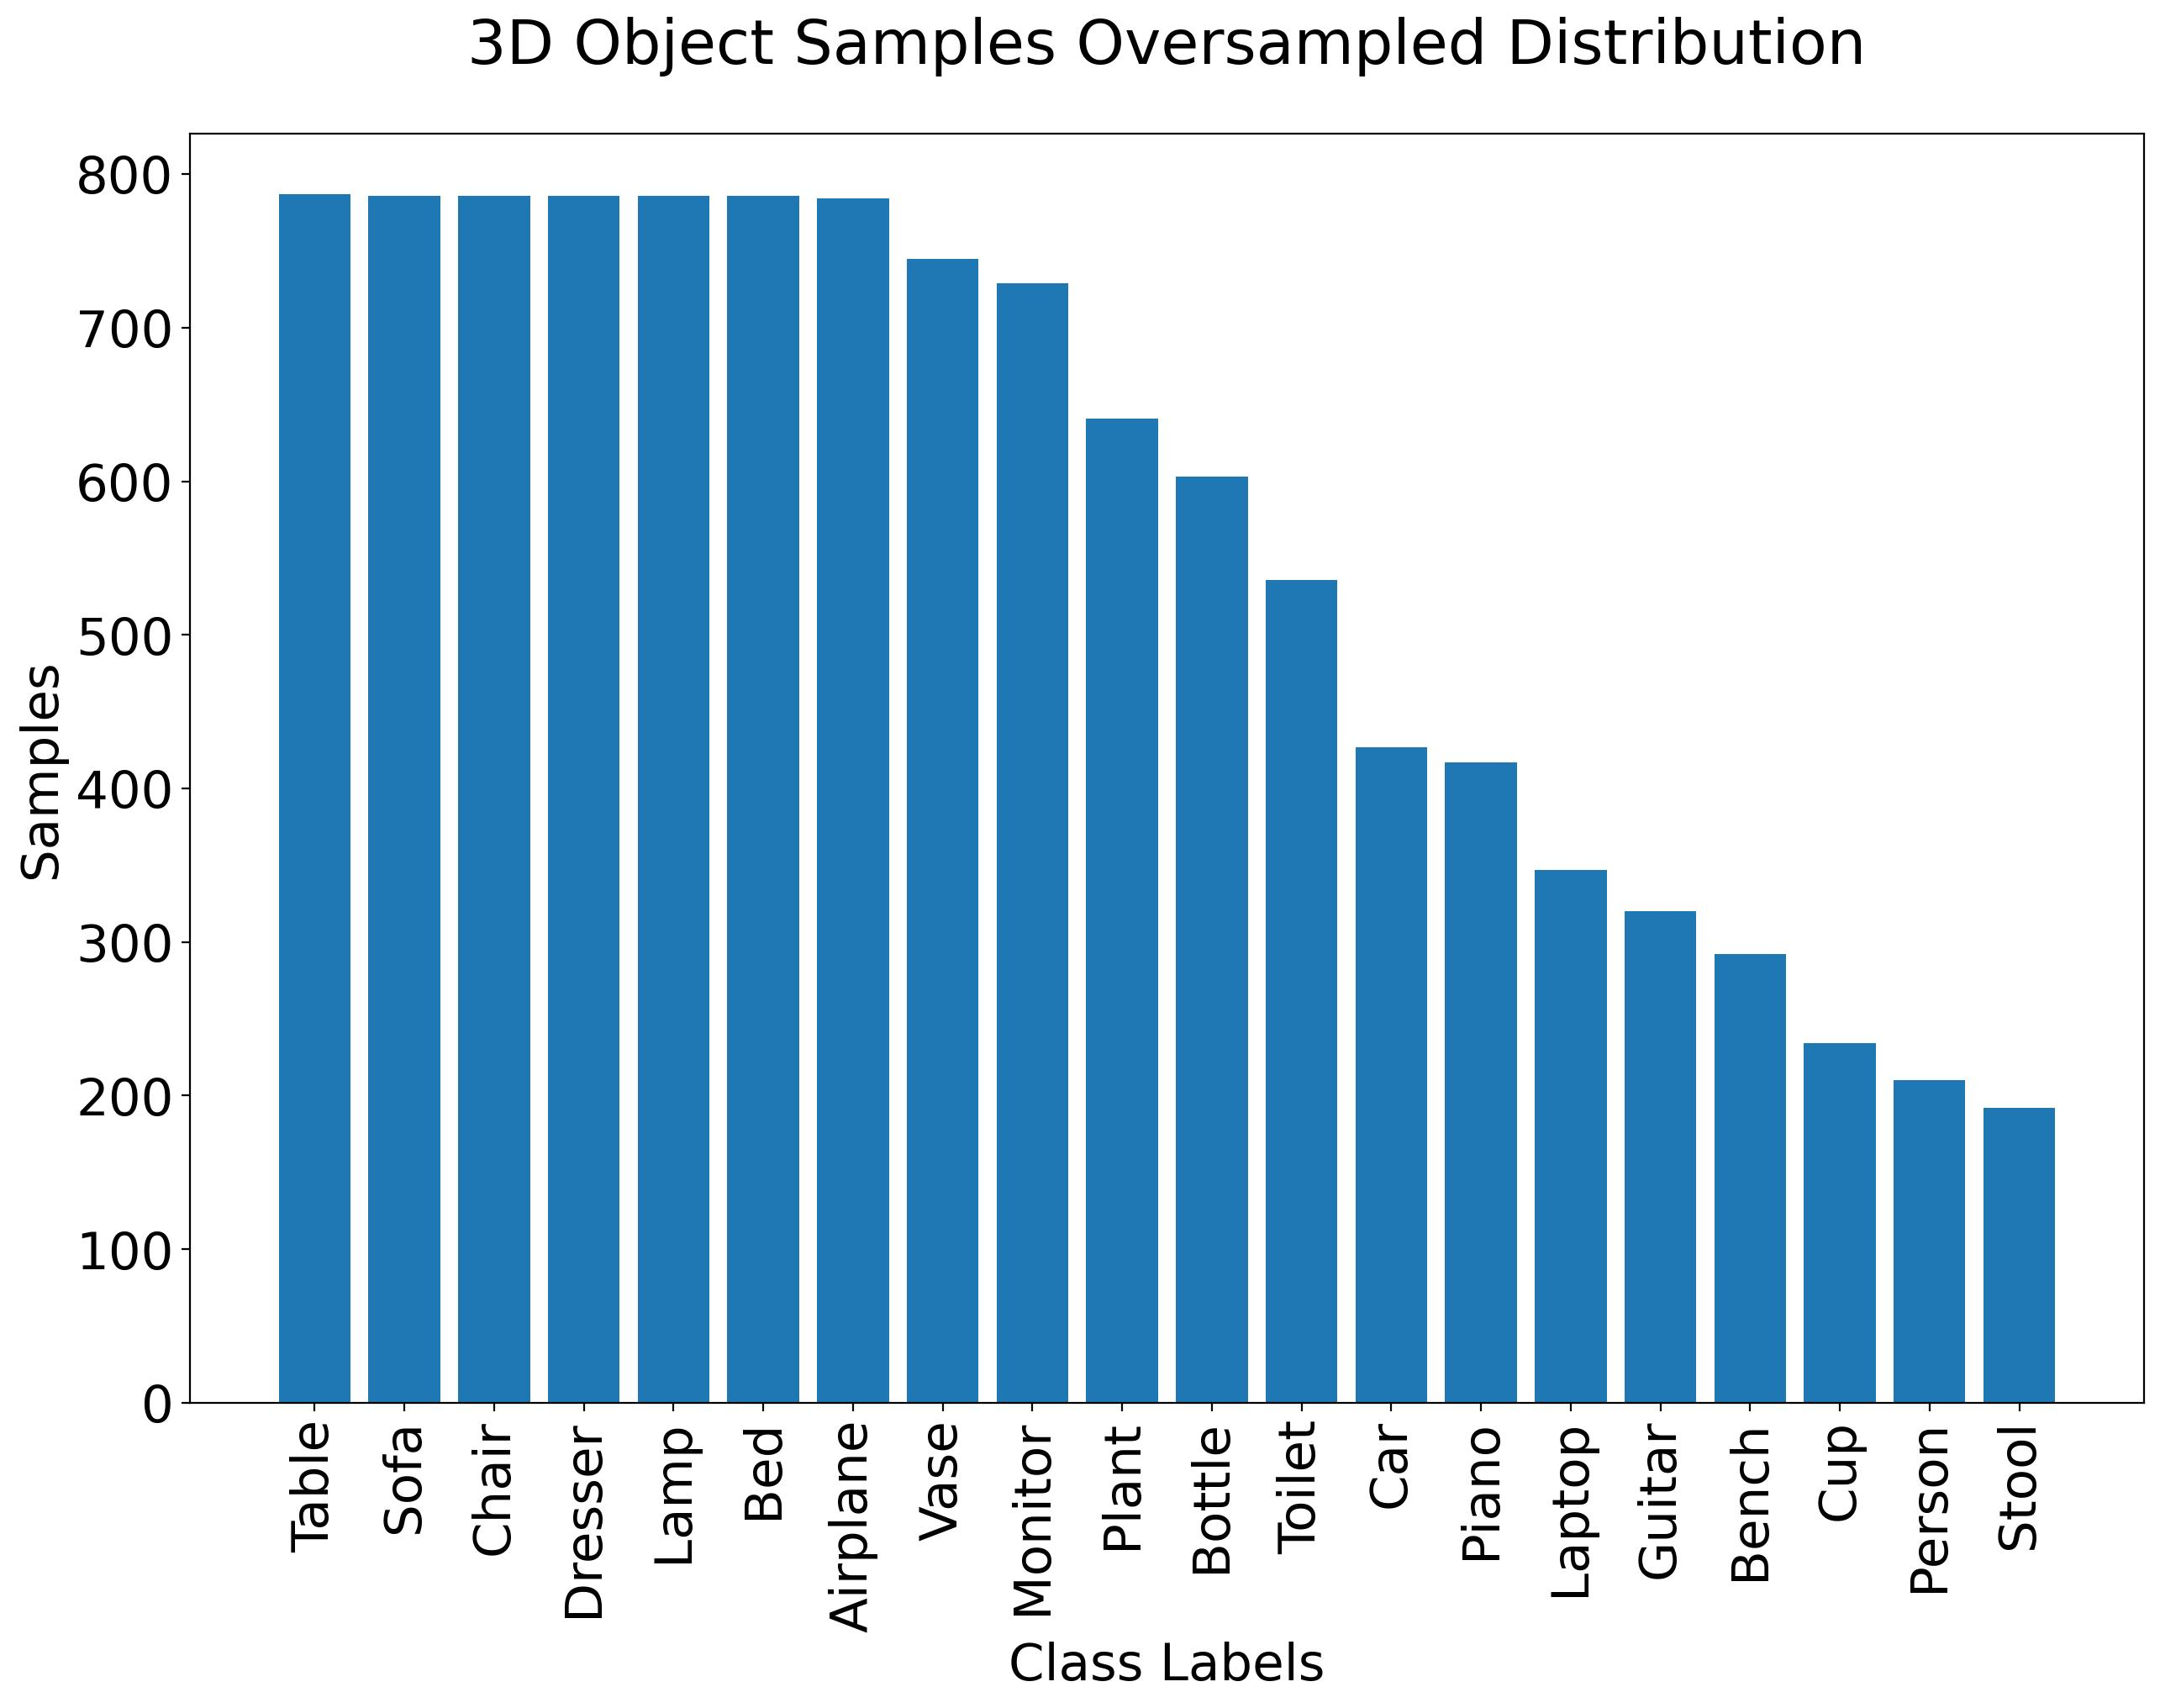
\includegraphics[scale=0.35]{imgs/3d-object-oversampled-distribution.jpg}
    \caption{3D Object Samples per class after oversampling}
\end{figure}
\noindent
A little bit of imbalance is still present, however it \textbf{is not easy to find point cloud data for exactly all the class labels of our interest}.\\
\\
As far as it concerns the RGB images, initially an attempt was made fetching content from
\begin{itemize}
    \item Caltech-101 (\url{http://www.vision.caltech.edu/Image_Datasets/Caltech101}),
    \item Caltech-256 (\url{http://www.vision.caltech.edu/Image_Datasets/Caltech256}),
    \item ImageNet (\url{https://www.image-net.org}),
    \item Open Images Dataset (\url{https://storage.googleapis.com/openimages}),
\end{itemize}
this approach however is limited by two main drawbacks:
\begin{itemize}
    \item the datasets provide images with too much noise (out of context picture with occlusions);
    \item the datasets do not contain the class labels of our interest;
\end{itemize}
As a result, the choice was made to use FastClass\footnote{\url{https://github.com/cwerner/fastclass}}: a tool to crawl search engines (Google, Bing, Baidu, Flickr) and pull all images for a defined set of queries. In addition, files are renamed, scaled and checked for duplicates.\\
After oversampling, this is the final result obtained:
\begin{figure}[H]
    \centering
    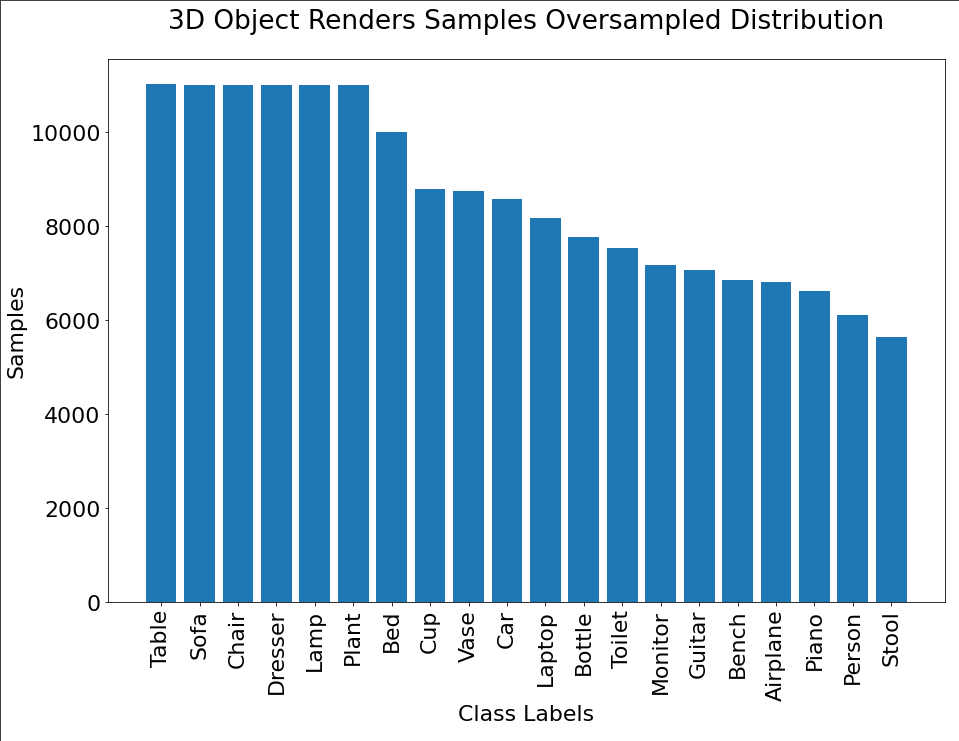
\includegraphics[scale=0.35]{imgs/3d-object-renders-crawling-oversampled-distribution.png}
    \caption{RGB Images (3D Objects Renders) per class after oversampling}
    \label{rgb-images-balancing}
\end{figure}
\noindent
By itself, crawling was not sufficient to fetch enough images to augment the RGB images. This is why I also used image transformations in order to augment the data. To this end, the \texttt{keras.preprocessing.image} package was used.\\
After oversampling, this is the final result obtained:
\begin{figure}[H]
    \centering
    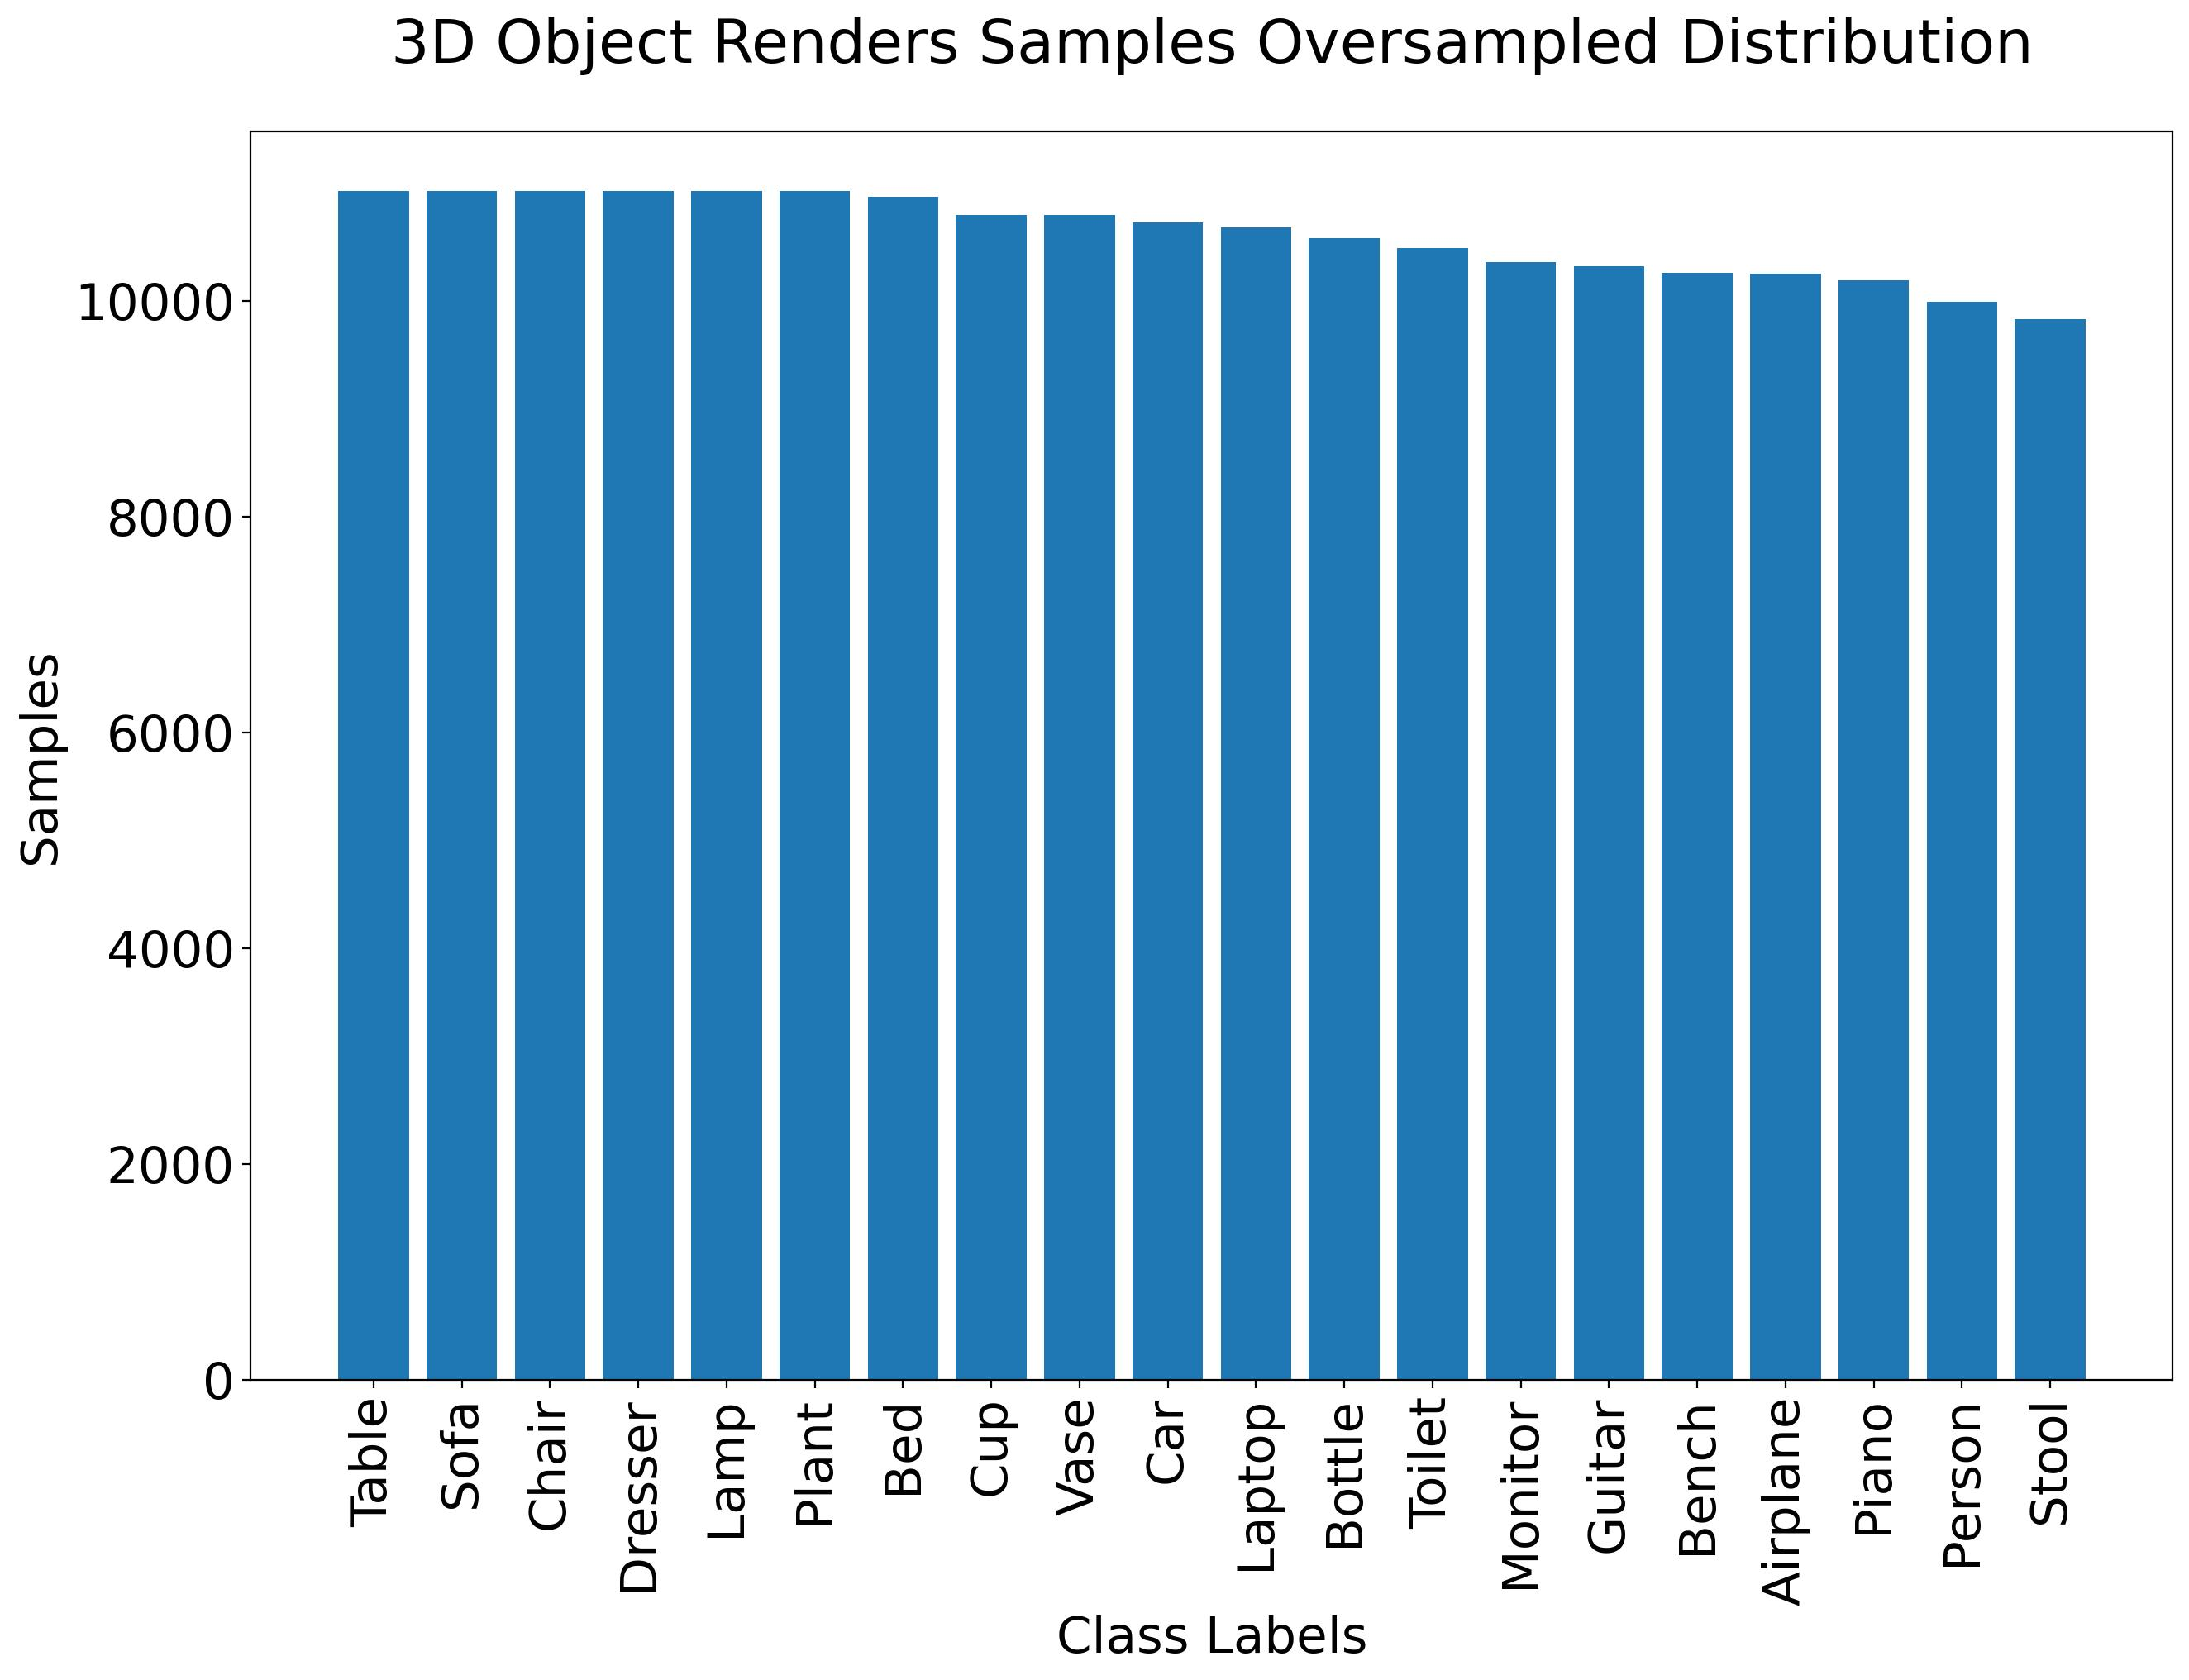
\includegraphics[scale=0.35]{imgs/3d-object-renders-transformations-oversampled-distribution.jpg}
    \caption{RGB Images (3D Objects Renders) per class after oversampling}
\end{figure}
\subsection{Final Class Labels}
Taking into account the entire preprocessing applied to the original dataset, the choice was done to focus the classification task on the top 5 categories of samples: \textbf{Table}, \textbf{Chair}, \textbf{Lamp}, \textbf{Dresser} and \textbf{Sofa}.
\begin{figure}[H]
    \centering
    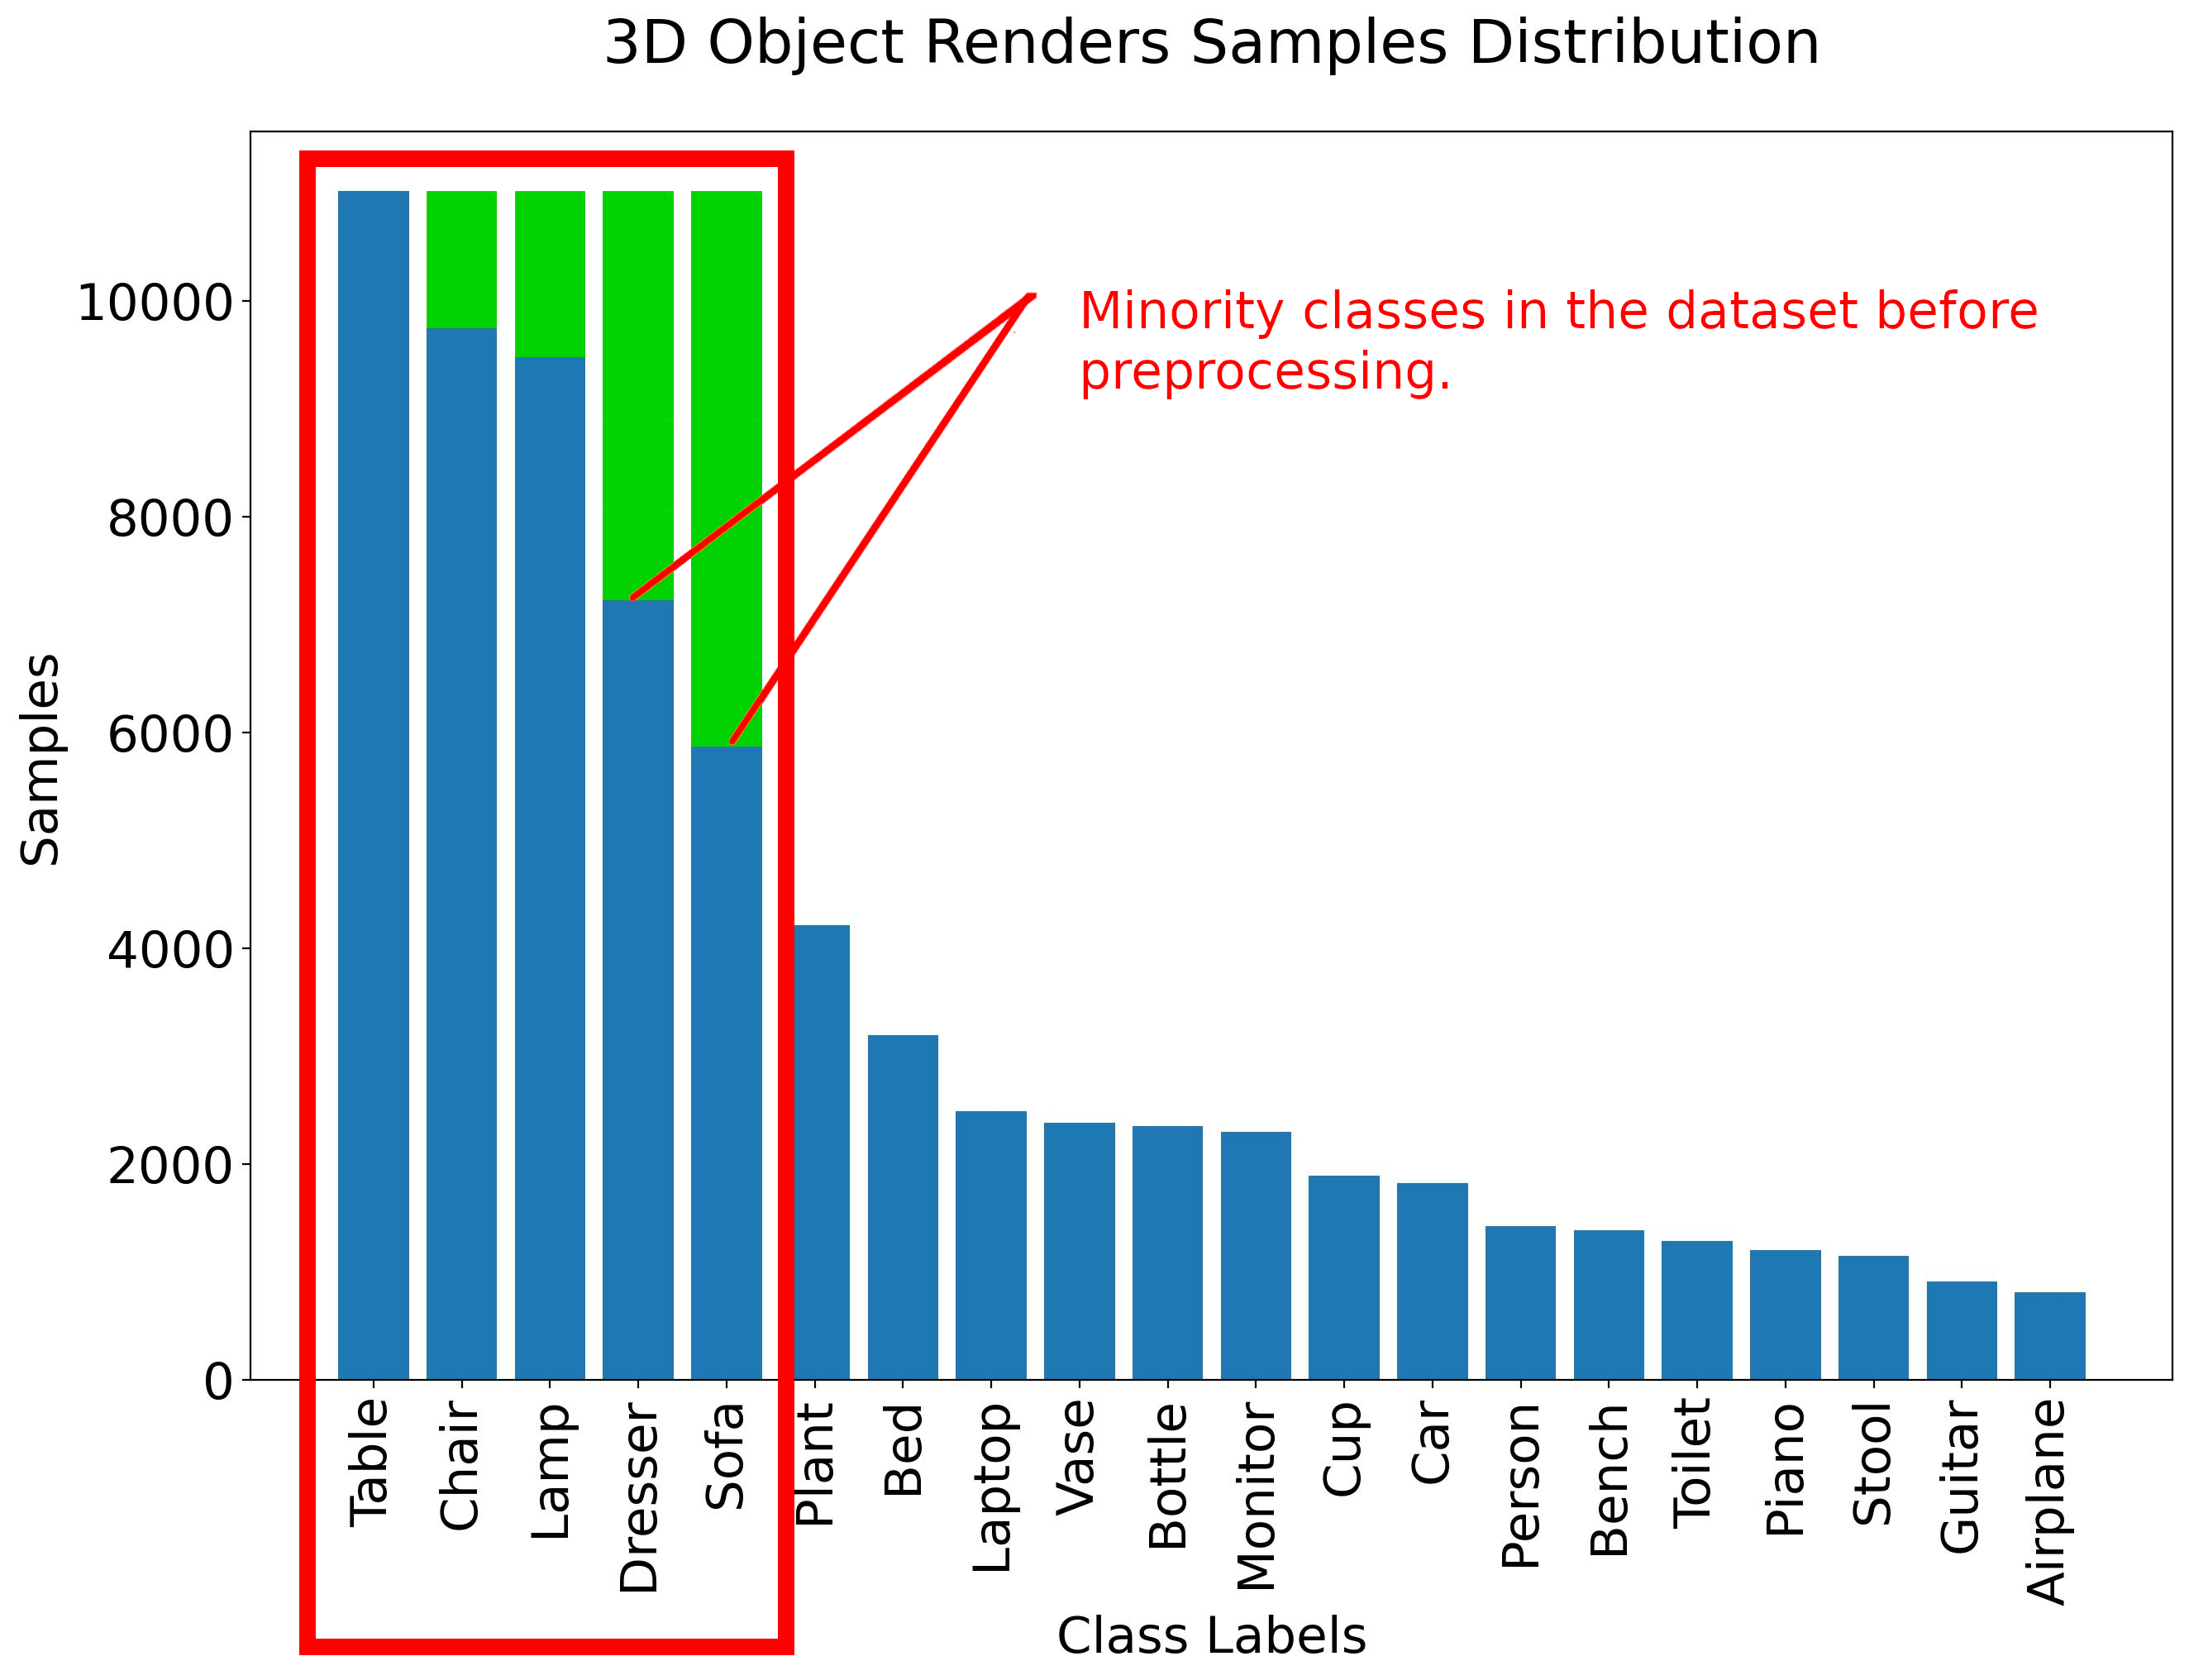
\includegraphics[scale=0.42]{imgs/selected-categories.jpg}
    \caption{Classes of objects for the classification task}
\end{figure}
This choice was made on the basis of the followings:
\begin{itemize}
    \item using too many categories will make the model classification results scores (confusion matrices, ROC curves, etc...) harder to comprehend;
    \item excessive data augmentation was used in order to achieve data balancing for the minor classes which might result in additional noise;
    \item the minority classes \textbf{Dresser} and \textbf{Sofa} were kept in order to be able to later analyse eventual side effects on classification accuracy due to the preprocessing step.
\end{itemize}
\subsection{Stratified K-Fold Cross Validation}
In order to obtain statistically significant results, Stratified K-Fold Cross Validation was implemented. There is no ready made implementation offered by \texttt{tensorflow.keras} that can be used in this case. A custom implementation was made which allows to generate \texttt{train}, \texttt{validation} and \texttt{test}.
\begin{figure}[H]
    \centering
    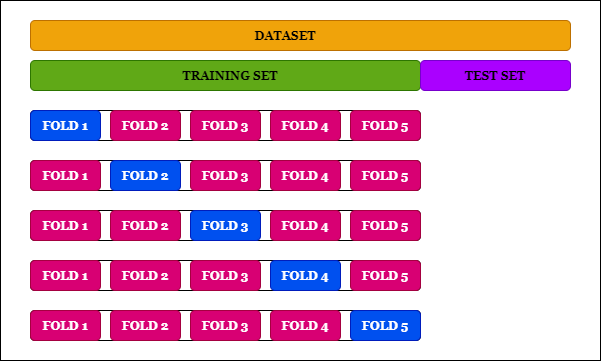
\includegraphics[scale=0.5]{imgs/train-validation-test.png}
\end{figure}
\noindent
The implementation used for the images and for the point clouds differs since the type of data and the loading procedure are different.
\subsubsection{Stratified K-Fold Cross Validation for images}
\begin{lstlisting}[language=Python,frame=single,caption={Definition of the function used to perform stratified K-Fold cross validation with images data.},captionpos=b]
def images_kfold_validation_model(model_name, n_splits, test_size, shuffle, model, learning_rate, decay, target_size, epochs, batch_size, one_fold=True, resample_data=0, augment=False):

...
\end{lstlisting}
The most important observations regarding this function include:
\begin{itemize}
    \item it takes as input the model name, layers, and parameters such as the number of folds, the learning rate, the decay rate, the number of epochs and the batch size;
    \item it defines the \texttt{StratifiedKFold} from the \texttt{sklearn.model\_selection} package;
    \item it instantiates the \texttt{ImageDataGenerator} from the \texttt{tf.keras.preprocessing.image} package needed to load the images;
    \item it defines the \texttt{tf.keras.callbacks.ModelCheckpoint} used to save the best model for each fold;
    \item it first generates the \textbf{test} and \textbf{train} folds; the train fold is then used to generate train and \textbf{validation} folds;
    \item it compiles the \texttt{tf.keras} model using the given layers;
    \item it trains and test the model plotting:
    \begin{itemize}
        \item train and validations sets accuracy and loss;
        \item confusion matrix computed on the test set;
        \item ROC curve for each class and average AUC;
    \end{itemize}
    \item new data generators are created in each iteration as the training data and the validation data changes;
    \item if specified, it perform sampling on the dataset in order to reduce the numerosity;
    \item it allows to perform "one fold" training; this was used for the initial experimental models in order to avoid to waste too much time;
    \item it is important to point out that \texttt{data augmentation} and \texttt{shuffling} are performed only on the \texttt{test set}; \texttt{data normalization} is performed on both \texttt{training}, \texttt{validation} and \texttt{testing} sets.
\end{itemize}
\subsubsection{Stratified K-Fold Cross Validation for point clouds}
Similarly, a utility function was written also for handling stratified K-Fold cross validation with point clouds. The main difference between the two is how the data is loaded and some initialization parameters:
\begin{lstlisting}[language=Python,frame=single,caption={Definition of the function used to perform stratified K-Fold cross validation with point clouds data.},captionpos=b]
    def pointclouds_kfold_validation_model(model_name, n_splits, test_size, shuffle, model, learning_rate, decay, target_size, epochs, batch_size, one_fold=True, resample_data=0, augment=False):

    ...
\end{lstlisting}
The \texttt{trimesh}\footnote{\url{https://github.com/mikedh/trimesh}} Python package was used in order to work with point cloud data:
\begin{itemize}
    \item it allows to load both \texttt{.obj} and \texttt{.off} 3D meshes;
    \item is allows to sample point clouds specifying the number of points;
    \item it allows for point clouds to be plotted using the \texttt{matplotlib.pyplot} package.
\end{itemize}
For the detailed implementation of the above mentioned functionalities please refer to the Jupyter Notebook named \texttt{KFold-Cross-Validation.ipynb}.
\subsection{Increased Computational Cost}
Before moving on, it is important to point out that when the first experiments were performed \textbf{using images} the computational cost required was too high. Such computational cost resulted from combining:
\begin{itemize}
    \item Stratified K-Fold Cross Validation;
    \item More than $50000$ images samples.
\end{itemize}
Consequently the following decisions were made:
\begin{itemize}
    \item Use Hold-out Validation and a dedicated \texttt{test} directory;
    \item Reduce the number of \textbf{training samples} to $\sim 10000$ ($\sim 2000$ per class);
    \item the \texttt{test} directory contains $\sim 1250$ ($\sim 250$ per class) \textbf{testing samples}.
\end{itemize}

\newpage
\section{Task 2: Training from scratch: Images}
The implementation of what is described in this section can be found in the Jupyter Notebook named \texttt{Task2-Training-from-scratch-images.ipynb}.\\
\\
This task focused on the development from scratch of an ad-hoc CNN to classify between the selected class labels (\textbf{Table}, \textbf{Chair}, \textbf{Lamp}, \textbf{Dresser} and \textbf{Sofa}) using both RGB images and 3D point clouds.\\
\\
In practice, applied Machine Learning is a highly iterative process. As a matter of fact, while our \textit{trainable parameters} (the weights) are obtained as a result of the training procedure, the hyperparameters must be provided as input to the training process. Even very experienced Deep Learning practitioners fail to get hyperparameters right the first time. The process is to turn the idea into code, experiment, and evaluate the outcome and make changes and repeat the process until you get the expected or otherwise a satisfactory outcome. In simpler words it is a trial and error process which can sometimes be helped by guidance found in the literature.\\
\\
In what follows, this trial and error process is described. Each of the following subsections is dedicated to one experiment and the results obtained. Starting from the obtained results, a new experiment is proposed and tested:
\begin{itemize}
    \item Hold-out Validation was used in order to generate \texttt{train}, \texttt{validation} and \texttt{test} sets; the \texttt{train} set was used to perform the training, the performance on the \texttt{validation} set was used in order to tune hyperparameters and the generalization capability of the model is shown by the performance on the \texttt{test} set;
    \item each model was trained for at least \texttt{50} epochs; the model with the lowest \texttt{validation loss} during the entire training process is saved as \texttt{best model}; the \texttt{best model} is tested on the test set;
    \item the initial experiments focused on tuning the \texttt{capacity} of the model; as soon as \texttt{overfitting} behavior is spotted, \texttt{regularization} techniques will be used to fight back;
    \item models for RGB images were trained using the \texttt{RMSprop} optimizer, loss function \texttt{categorical\_crossentropy} and \texttt{accuracy} metric;
\end{itemize}
\subsection{Target Size}
Before jumping straight into the training procedure and experimenting, some statistical data collection was performed on the images in the dataset in order to find the proper target input size. Here, by "proper size", it is meant the width and the height to be used (passed as arguments to the \texttt{ImageDataGenerator}) for loading the images so as to reduce distortions.
\begin{lstlisting}[language=Python,frame=single]
images_sizes = []
for image_filename in images_X['filename']:
    if image_filename != 'filename':
        image = Image.open(image_filename)
        images_sizes.append(image.size)

images_sizes = numpy.array(images_sizes)

print("Loaded images: " + str(len(images_sizes)))
print("Average size: " + str(numpy.average(images_sizes, axis=0)))
\end{lstlisting}
\begin{lstlisting}[language=bash,frame=single]
Loaded images: 9270
Average size: [512. 512.]
\end{lstlisting}
The choice was made to use the input size $(128, 128)$. This choice was guided also by the literature \cite{DBLP:journals/corr/abs-2101-11508} \cite{effectofimagesize}: 
\begin{displayquote}
\textit{"Higher order features which are essential to distinguish images between classes having similarities are removed as a result of image rescaling. Maintaining a  higher image  size enabled models to achieve a  flatter loss function, highly suggestive of the  fact  that  such  models  generalize  better. This however increases the computation time hence a trade-off is inevitable."}
\end{displayquote}
The experiments performed on the dataset of RGB images are now presented.
\subsection{Experiment 0 - Simple Model}
The best place where to start is with the simplest model possible, so simple that we can consider it a naive experiment. At this stage, we are mainly focused in finding the \textit{capacity} of our model, that is the number of hidden layers and the number of hidden units per hidden layer to be used in our CNN.\\
The model is made of $2$ convolutional layers interleaved with max-pooling, and after a fully connected layer with $32$ units, the output layer is obtained using $5$ neurons with \texttt{softmax} activation:
\begin{lstlisting}[language=Python,frame=single]
# experiment model layers
layers = [
    Conv2D(32, (3, 3), 'relu', (128, 128, 3)),
    MaxPooling2D((2, 2)),
    Conv2D(64, (3, 3), 'relu'),
    MaxPooling2D((2, 2)),
    Flatten(),
    Dense(32, 'relu'),
    Dense(NUM_CLASSES, 'softmax')
]

# train, validate and test
images_kfold_validation_layers(model_name="Experiment-0", n_splits=6,
        test_size=0.01, shuffle=True, layers=layers, learning_rate=0.001,
        decay=1e-6, target_size=TARGET_SIZE, epochs=50, batch_size=32,
        one_fold=True, resample_data=0, augment=False)
\end{lstlisting}
Default training hyperparameters (\texttt{learning rate}, \texttt{decay}, etc...) of the \texttt{RMSprop} implementation were used. Contrary to what I expected, this simple model \textbf{overfitted} the dataset with almost $10,000$ samples quite rapidly.\\
Using the \texttt{validation loss} as the monitored parameter during the training stage, the following results were obtained:
\begin{figure}[H]
    \centering
    \subfloat[\centering Loss]{{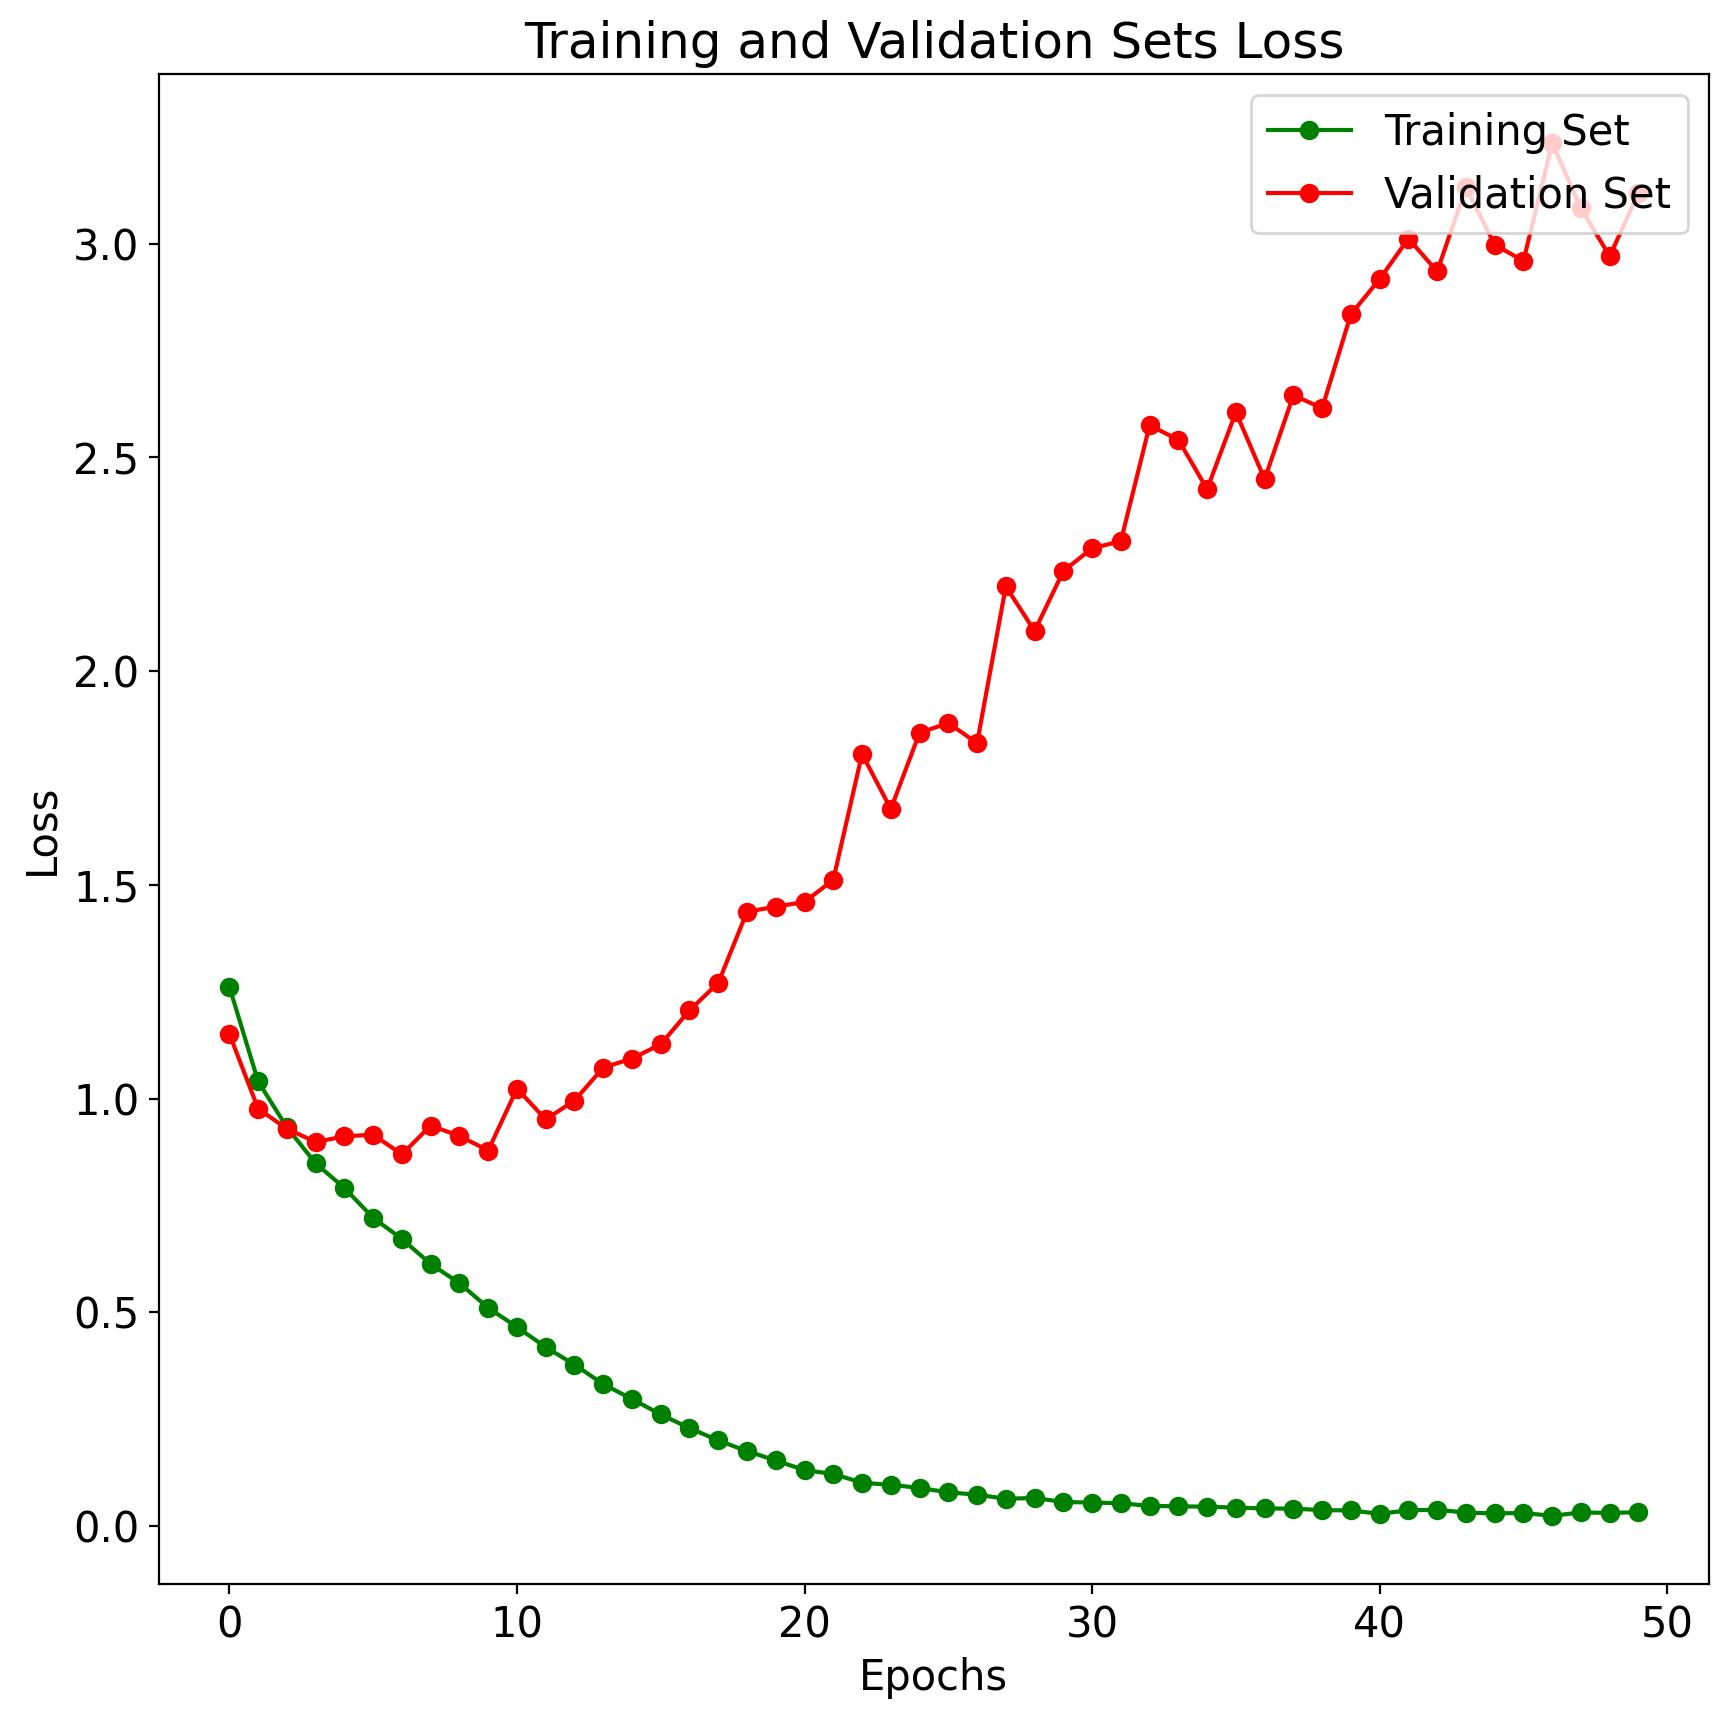
\includegraphics[scale=0.31]{imgs/experiments/images/0/Experiment-0-fold-1.h5-train-val-loss.jpg} }}
    \qquad
    \subfloat[\centering Accuracy]{{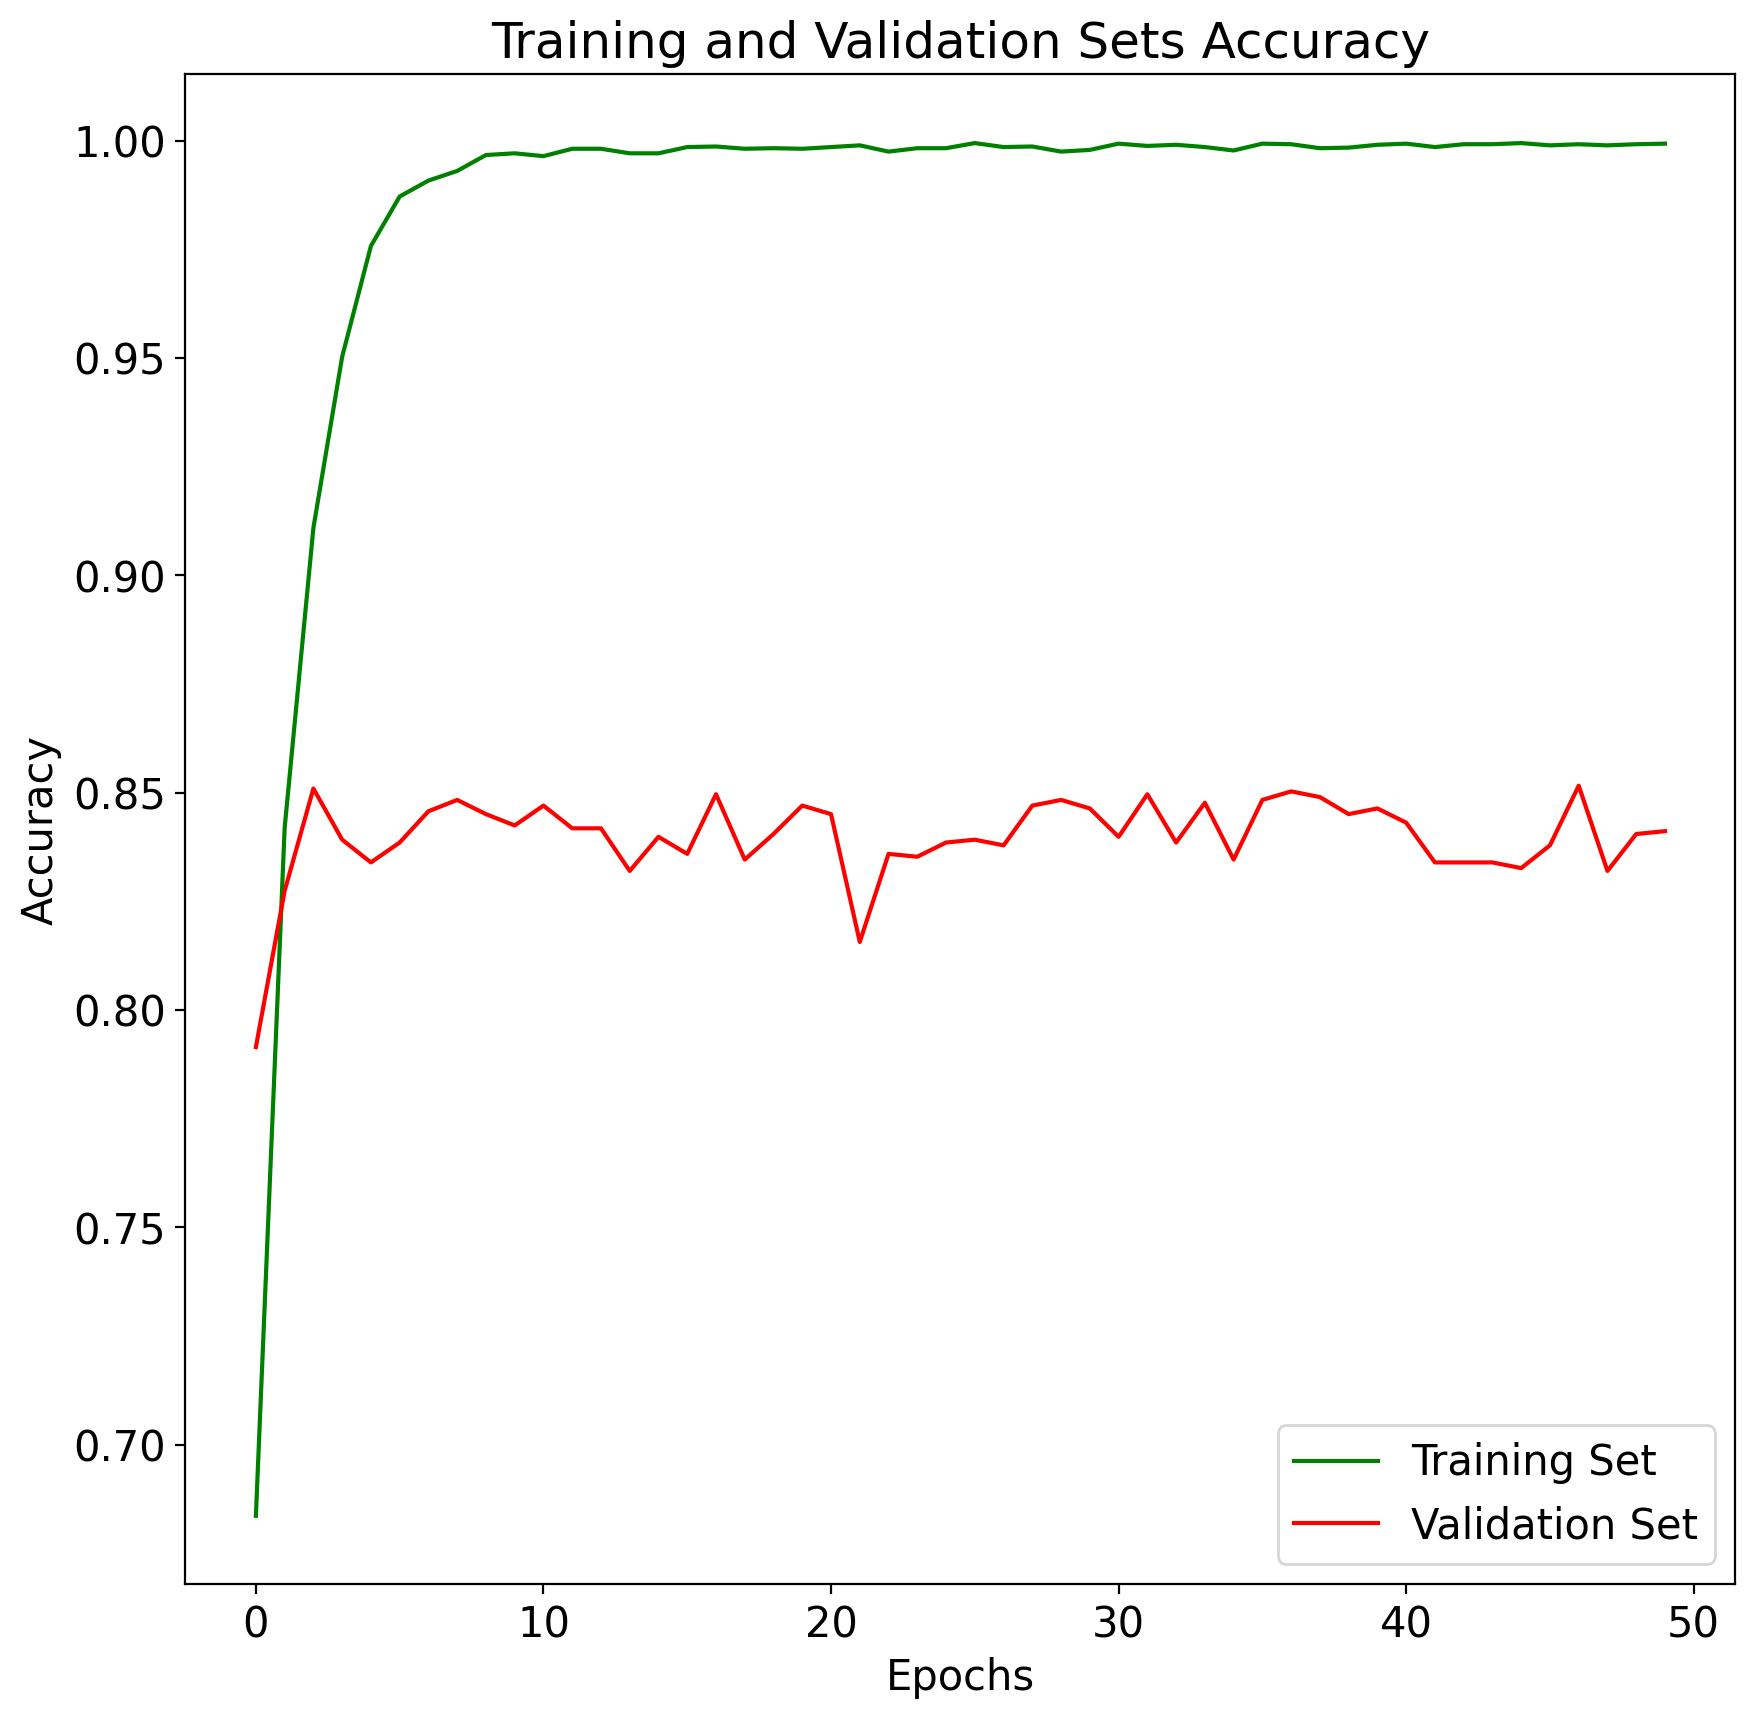
\includegraphics[scale=0.31]{imgs/experiments/images/0/Experiment-0-fold-1.h5-train-val-accuracy.jpg} }}
    \caption{Experiment 0 Results}
\end{figure}
\begin{center}
\begin{tabular}{|p{1.2cm}|p{1.8cm}|p{2cm}|p{2cm}|p{2cm}|p{2cm}|p{2cm}|}
\rowcolor{gray!50}
\hline
\textbf{Epoch} & \textbf{Training Loss} & \textbf{Training Accuracy} & \textbf{Validation Loss} & \textbf{Validation Accuracy}\\
\hline
$2$ & $0.4624$ & $0.8419$ & $0.5067$ & $0.8275$\\
\hline
\end{tabular}\\
\end{center}
Some of the conclusions we can draw from this experiment, include:
\begin{itemize}
    \item the simplest network is capable of overfitting the data after less than $10$ epochs; indeed, the shapes we are trying to classify are not that rich of particularities (the selected classes include tables, chairs, lamp, dressers and couches);
    \item neither dropout, nor data augmentation, nor regularization was used; which explains the overfitting phenomena;
\end{itemize}
\subsection{Experiment 1 - Dropout}
A simple and powerful regularization technique for neural networks and deep learning models is dropout. Dropout is a regularization technique for neural network models proposed by Srivastava, et al. in their 2014 paper \cite{JMLR:v15:srivastava14a}. Dropout is a technique where randomly selected neurons are ignored during training. They are “dropped-out” randomly. As a neural network learns, neuron weights settle into their context within the network. Weights of neurons are tuned for specific features providing some specialization. Neighboring neurons become to rely on this specialization, which if taken too far can result in a fragile model too specialized to the training data. Given the limited benefits when applied to convolutional layers \cite{DBLP:journals/corr/abs-1810-12890}, often dropout is only used after the dense fully connected layer; the choice was made to follow this heuristic:
\begin{lstlisting}[language=Python,frame=single]
# experiment model layers
layers = [
    Conv2D(32, (3, 3), 'relu', (128, 128, 3)),
    MaxPooling2D((2, 2)),
    Conv2D(64, (3, 3), 'relu'),
    MaxPooling2D((2, 2)),
    Flatten(),
    Dense(32, 'relu'),
    Dropout(0.4),
    Dense(NUM_CLASSES, 'softmax')
]

# train, validate and test
images_kfold_validation_layers(model_name="Experiment-1", n_splits=6,
        test_size=0.01, shuffle=True, layers=layers, learning_rate=0.001,
        decay=1e-6, target_size=TARGET_SIZE, epochs=50, batch_size=32,
        one_fold=True, resample_data=0, augment=False)
\end{lstlisting}
The dropout rate is set to $40\%$.
\begin{figure}[H]
    \centering
    \subfloat[\centering Loss]{{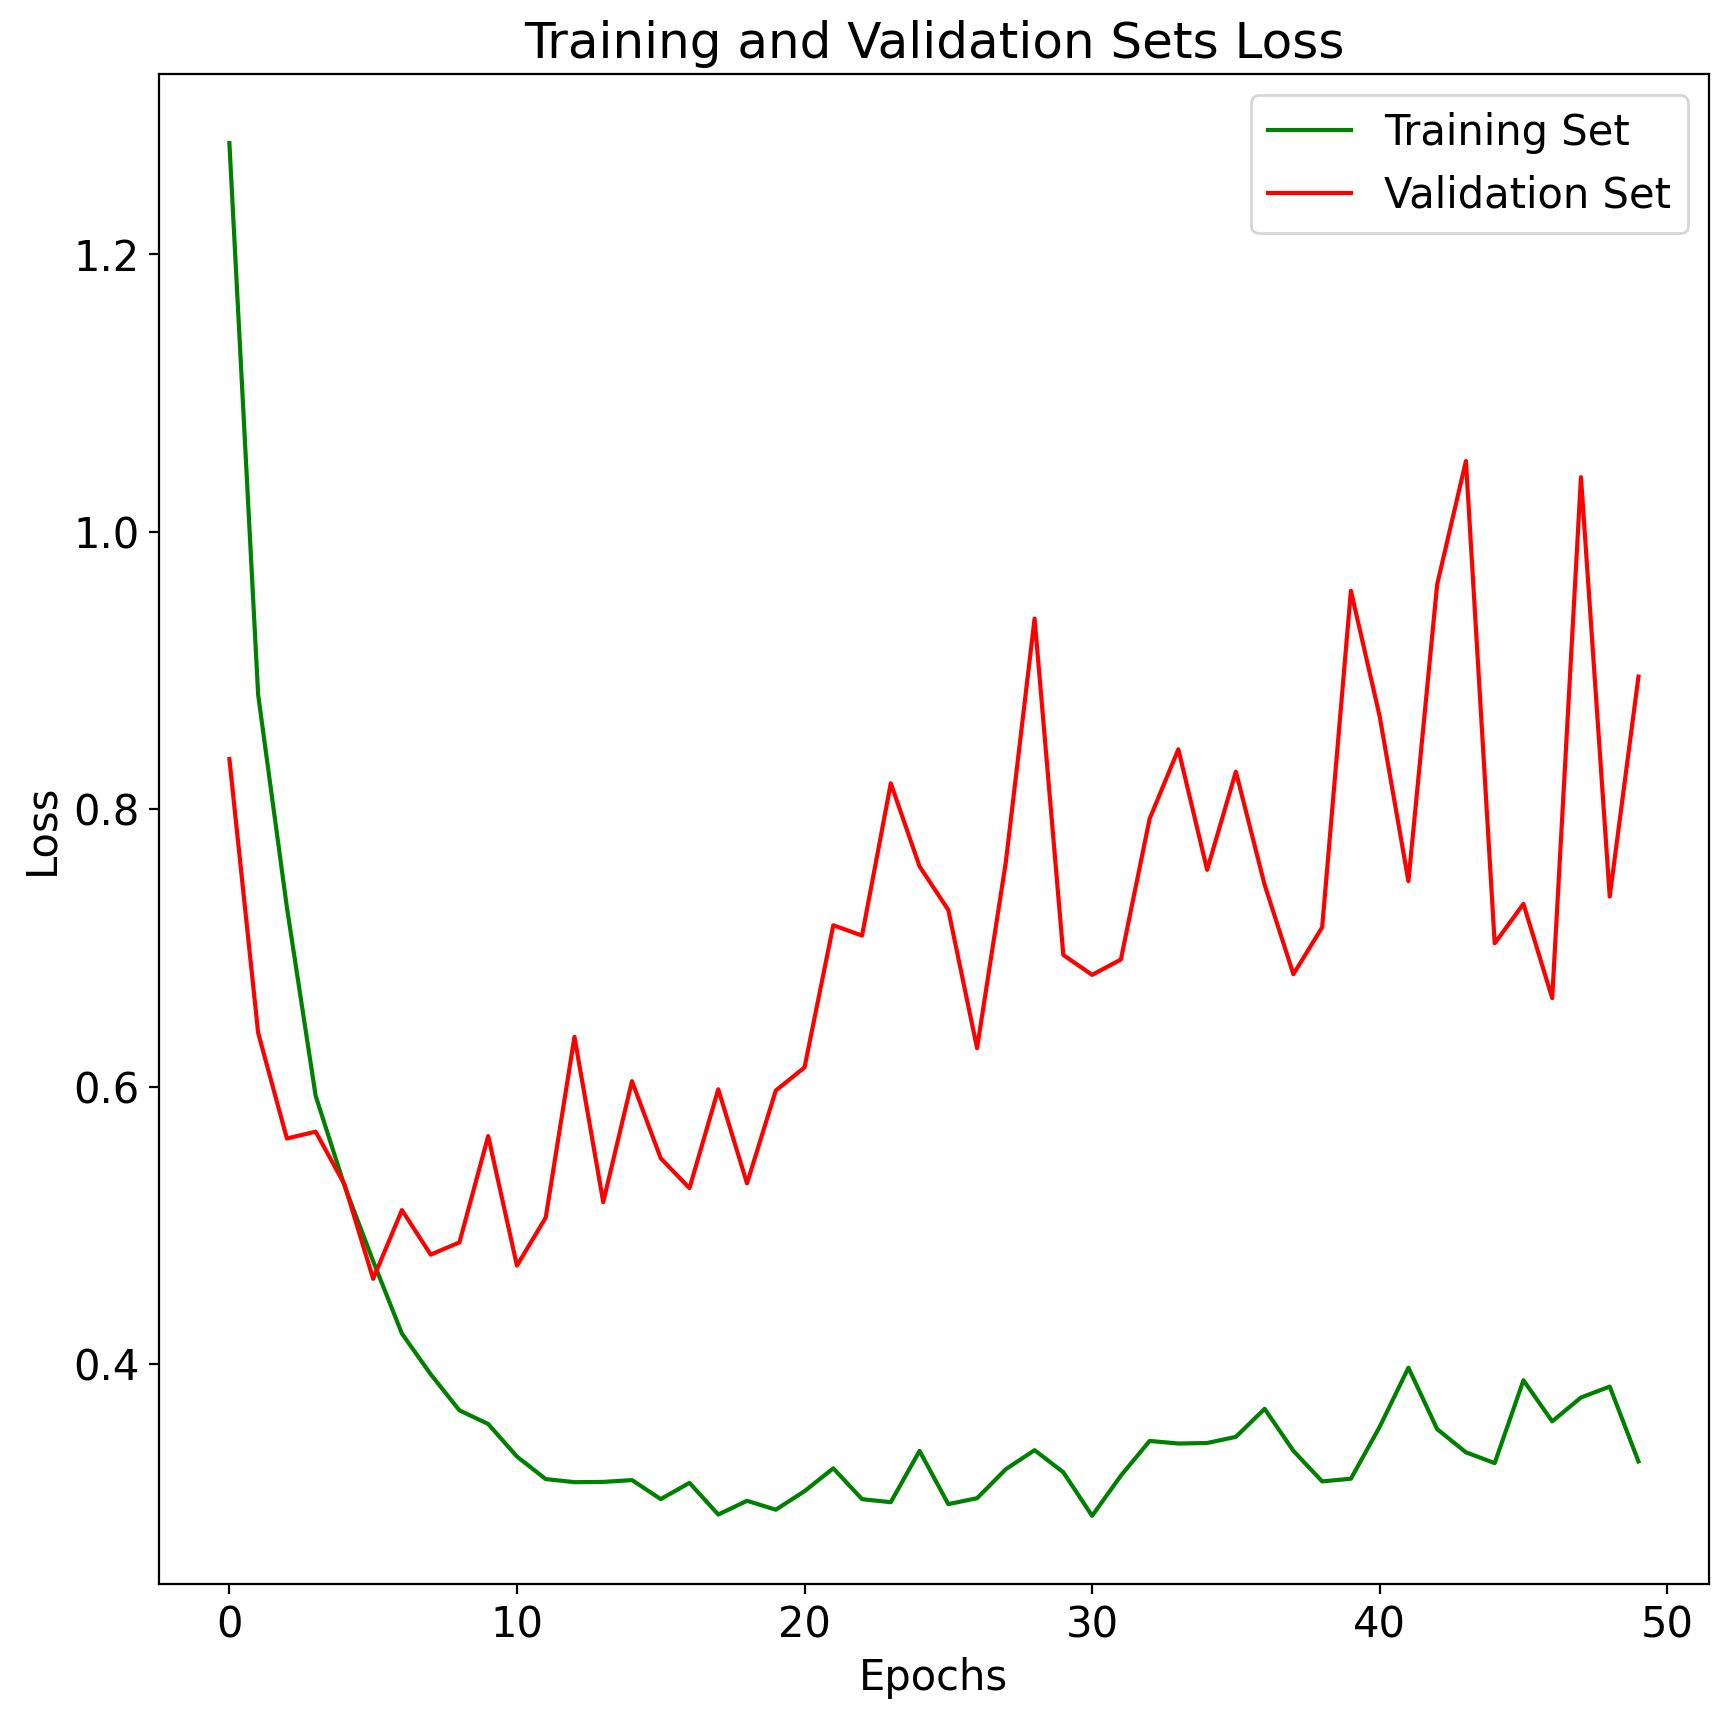
\includegraphics[scale=0.31]{imgs/experiments/images/1/Experiment-1-fold-1.h5-train-val-loss.jpg} }}
    \qquad
    \subfloat[\centering Accuracy]{{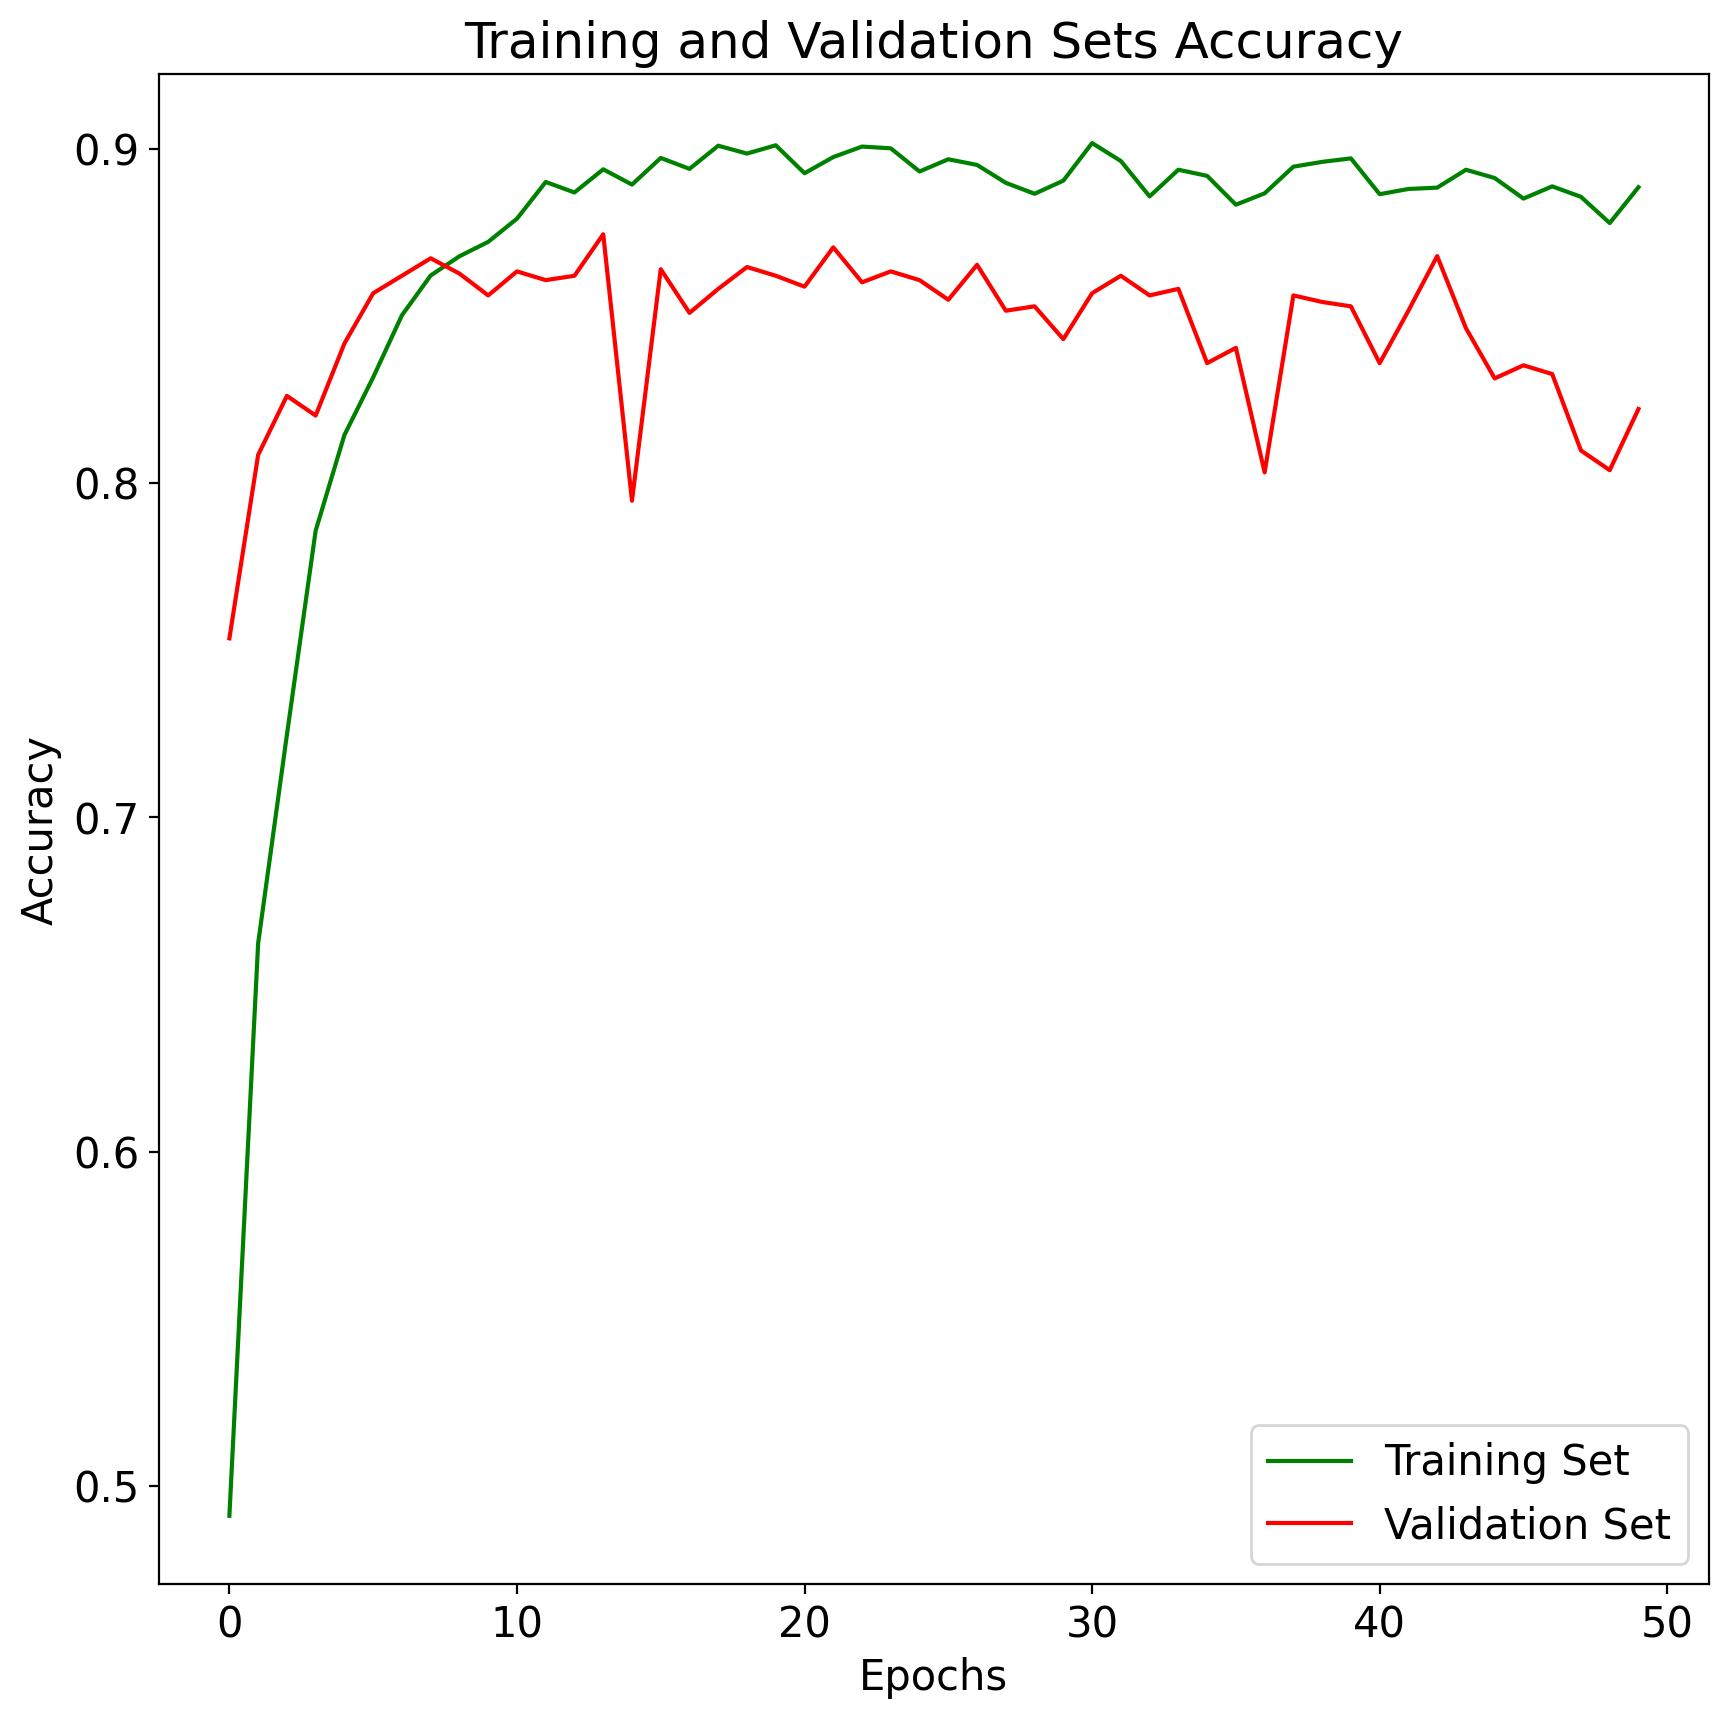
\includegraphics[scale=0.31]{imgs/experiments/images/1/Experiment-1-fold-1.h5-train-val-accuracy.jpg} }}
    \caption{Experiment 1 Results}
\end{figure}
\begin{center}
\begin{tabular}{|p{1.2cm}|p{1.8cm}|p{2cm}|p{2cm}|p{2cm}|p{2cm}|p{2cm}|}
\rowcolor{gray!50}
\hline
\textbf{Epoch} & \textbf{Training Loss} & \textbf{Training Accuracy} & \textbf{Validation Loss} & \textbf{Validation Accuracy}\\
\hline
$6$ & $0.4741$ & $0.8317$ & $0.4614$ & $0.8569$\\
\hline
\end{tabular}\\
\end{center}
Some of the conclusions we can draw from this experiment, include:
\begin{itemize}
    \item with respect to the previous experiment, using dropout avoids $100\%$ overfitting, and the accuracy on the validation set increase by a couple of percentage points;
    \item yet the \texttt{loss} on the validation set appears to be increasing epoch after epoch;
\end{itemize}
\subsection{Experiment 2 - Larger Model}
Given that with the use of dropout the model of the previous experiment could not achieve $100\%$ accuracy even on the training set, I decided to change the architectural layout to increase its capacity:
\begin{itemize}
    \item one additional convolutional block was added;
    \item the number of units of the fully-connected layer was doubled in order to better cope with the increased filters.
\end{itemize}
\begin{lstlisting}[language=Python,frame=single]
# experiment model layers
layers = [
    Conv2D(32, (3, 3), 'relu', (128, 128, 3)),
    MaxPooling2D((2, 2)),
    Conv2D(64, (3, 3), 'relu'),
    MaxPooling2D((2, 2)),
    Conv2D(128, (3, 3), 'relu'),
    MaxPooling2D((2, 2)),
    Flatten(),
    Dense(64, 'relu'),
    Dropout(0.4),
    Dense(NUM_CLASSES, 'softmax')
]

# train, validate and test
images_kfold_validation_layers(model_name="Experiment-2", n_splits=6,
    test_size=0.01, shuffle=True, layers=layers, learning_rate=0.001,
    decay=1e-6, target_size=TARGET_SIZE, epochs=50, batch_size=32,
    one_fold=True, resample_data=0, augment=False)
\end{lstlisting}
After $50$ epochs of training the following results were obtained:
\begin{figure}[H]
    \centering
    \subfloat[\centering Loss]{{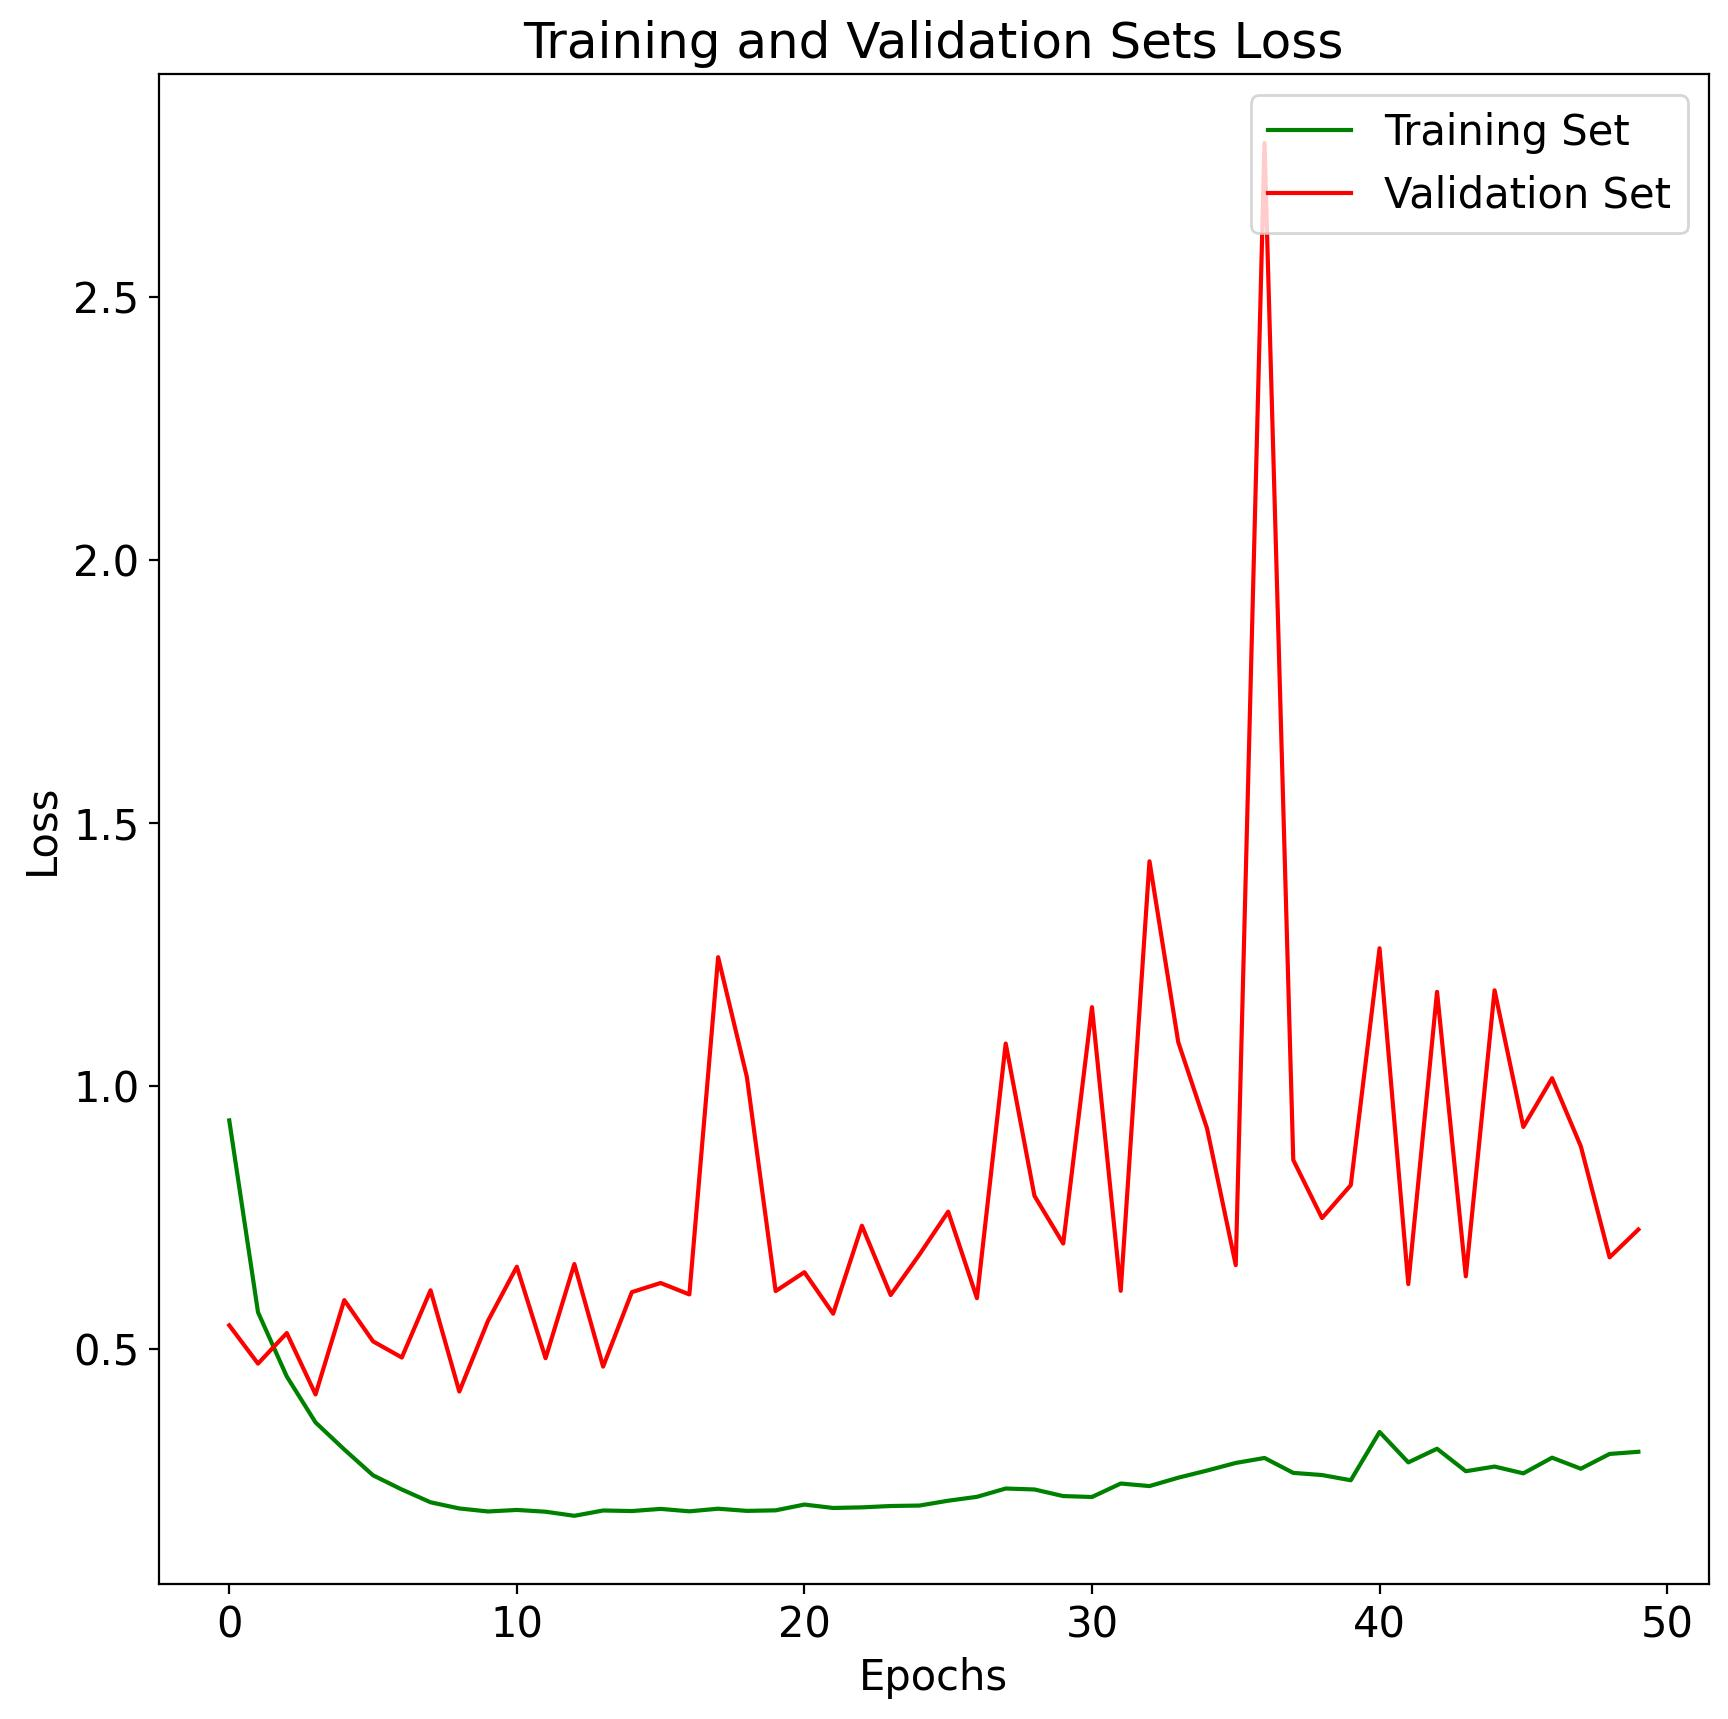
\includegraphics[scale=0.31]{imgs/experiments/images/2/Experiment-2-fold-1.h5-train-val-loss.jpg} }}
    \qquad
    \subfloat[\centering Accuracy]{{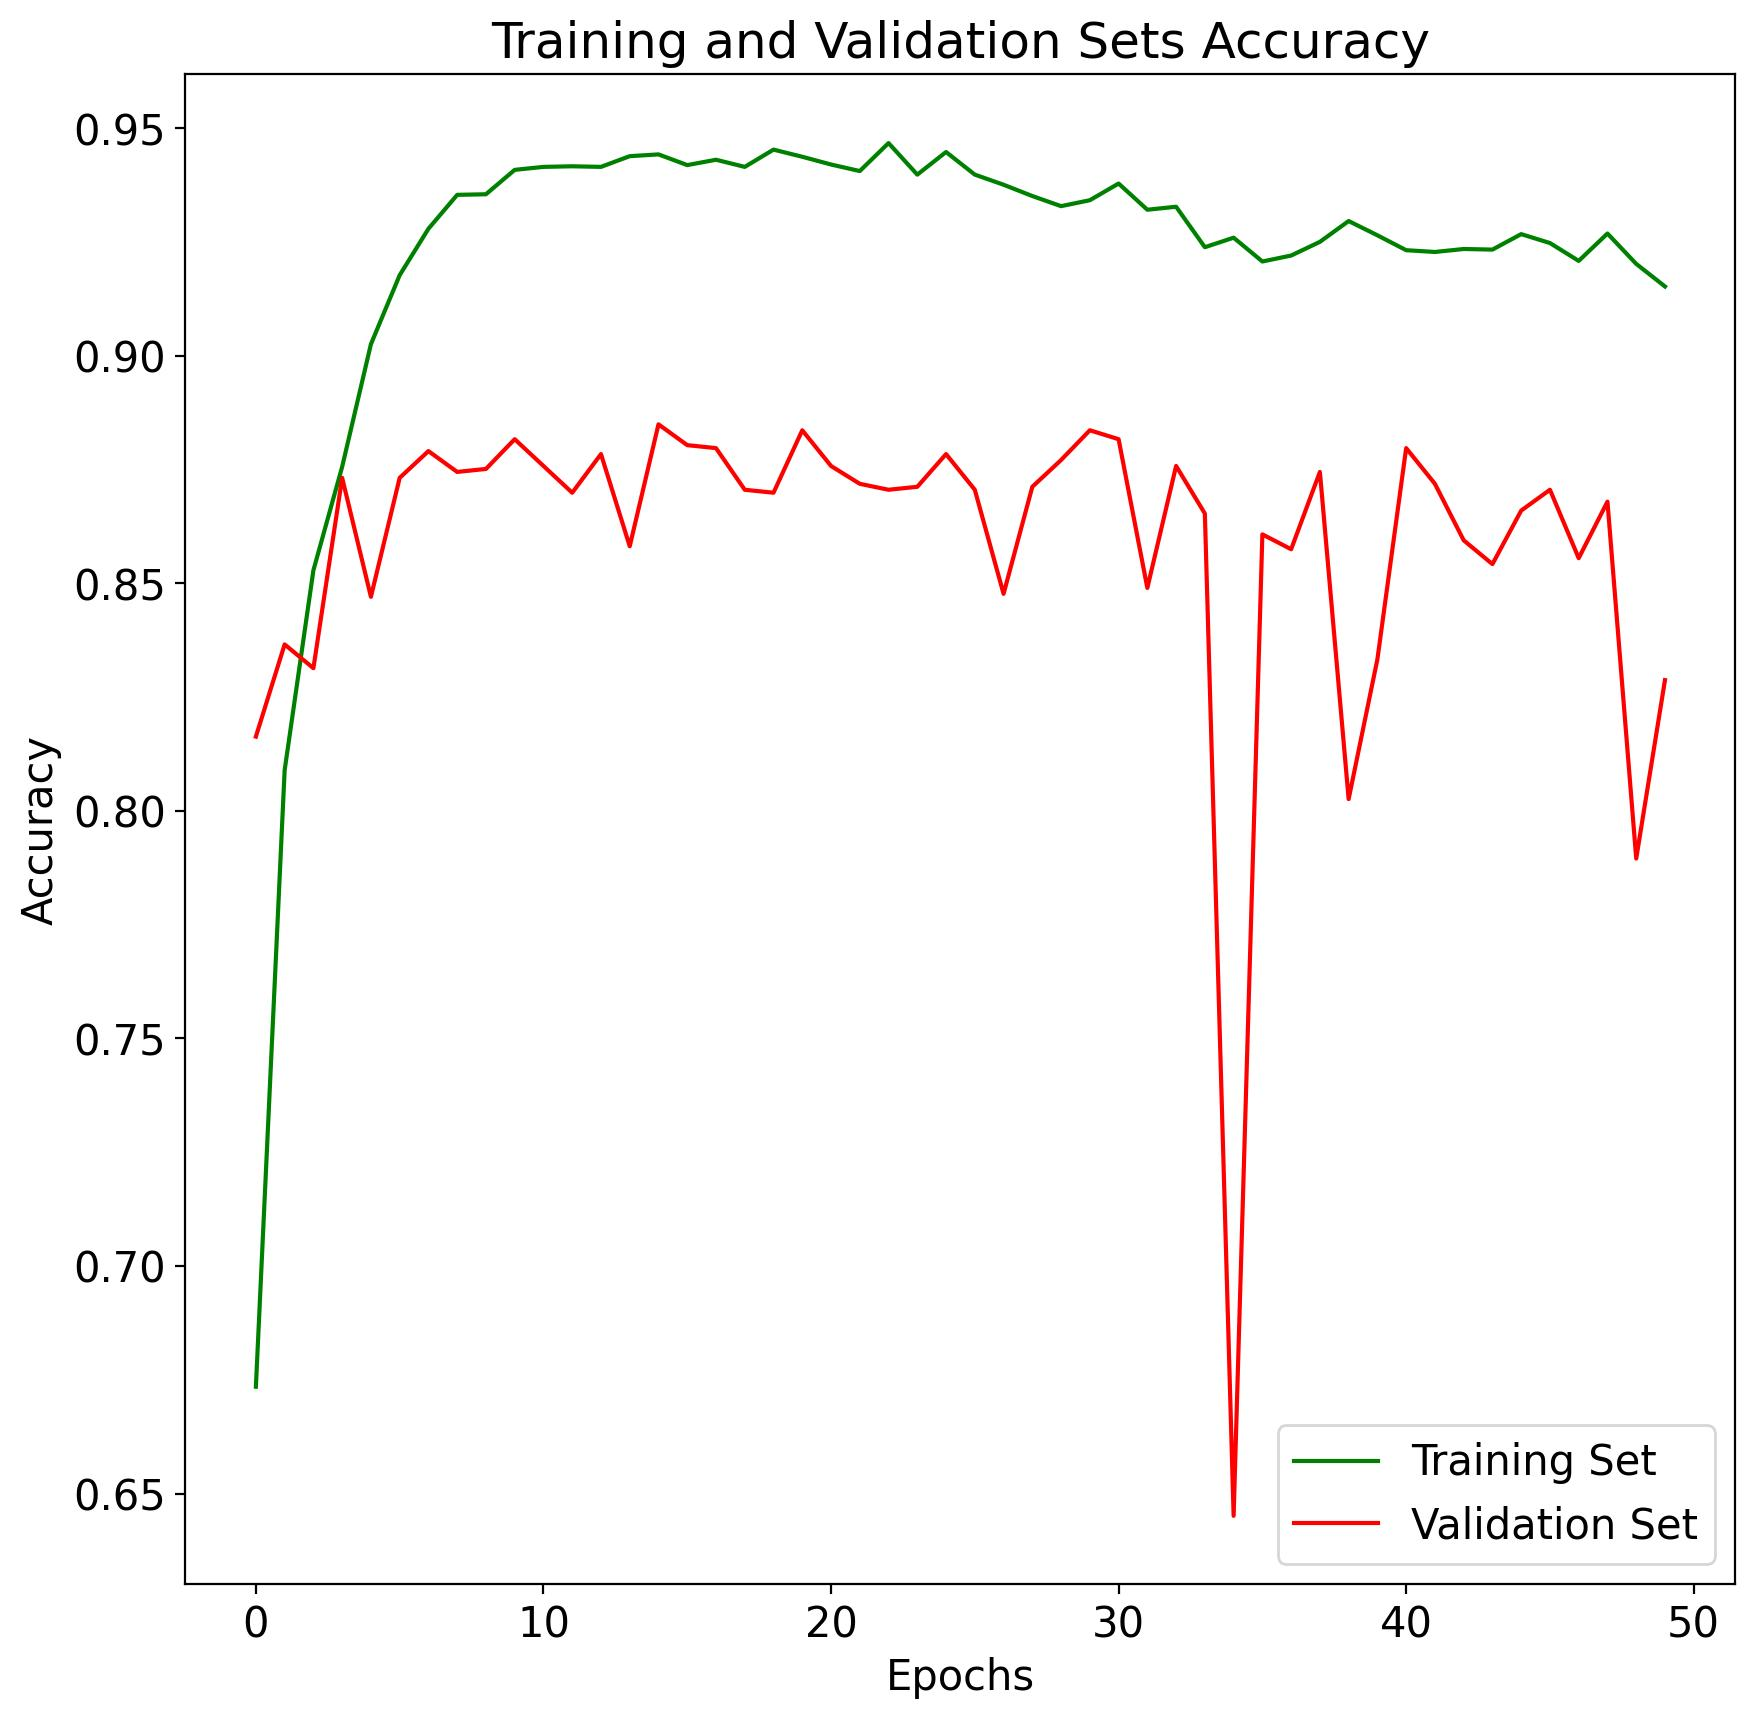
\includegraphics[scale=0.31]{imgs/experiments/images/2/Experiment-2-fold-1.h5-train-val-accuracy.jpg} }}
    \caption{Experiment 2 Results}
\end{figure}
\begin{center}
\begin{tabular}{|p{1.2cm}|p{1.8cm}|p{2cm}|p{2cm}|p{2cm}|p{2cm}|p{2cm}|}
\rowcolor{gray!50}
\hline
\textbf{Epoch} & \textbf{Training Loss} & \textbf{Training Accuracy} & \textbf{Validation Loss} & \textbf{Validation Accuracy}\\
\hline
$4$ & $0.3599$ & $0.8756$ & $0.4131$ & $0.8732$\\
\hline
\end{tabular}\\
\end{center}
Some of the conclusions we can draw from this experiment, include:
\begin{itemize}
    \item overall accuracy increased on training and validation sets;
    \item overfitting is still affecting the training process and this ends up ultimately ruining the overall performance of the model;
    \item abrupt variations are found on the validation sets scores;
    \item the accuracy on the training set appears to be decreasing; this negative slope is to be investigated.
\end{itemize}
\subsection{Experiment 3 - Data Augmentation, Longer Training}
To keep fighting overfitting, another regularization technique is applied to the model: \textit{data augmentation}. This consists in increasing the diversity of the training set by applying random (but realistic) transformations, such as image rotation, rescaling, horizontal and vertical flips. The following data augmentation tecniques were used:
\begin{itemize}
    \item random rotations in the range $[0^{\circ}, 180^{\circ}]$;
    \item horizontal and vertical random shift of pixels in the range $[-0.01, +0.01]$\footnote{In order to find the proper values for these parameters more than one experiment was performed. With too much data augmentation the learning rate of the model was too low and the maximum accuracy could not increase above a certain threshold. As a result, Early Stopping was terminating the learning process after $60$ epochs due to no improvement in the validation accuracy metric.} as percentage of teh actual width and height of the image ($128px$);
    \item random zoom in the range $[0.7, 1.3]$;
    \item random horizontal flip.
\end{itemize}
\begin{figure}[H]
    \centering
    \subfloat{{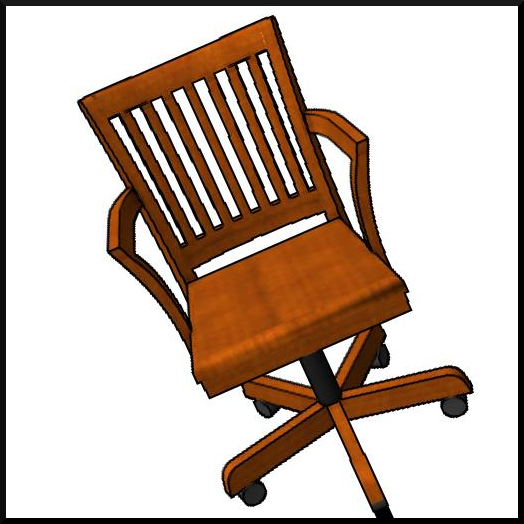
\includegraphics[scale=0.7]{imgs/data_augmentation/pic_0_9119.jpeg} }}
    \qquad
    \subfloat{{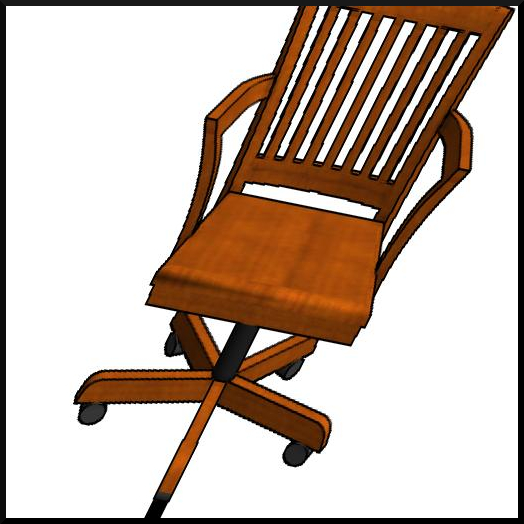
\includegraphics[scale=0.7]{imgs/data_augmentation/pic_0_9472.jpeg} }}
    \qquad
    \subfloat{{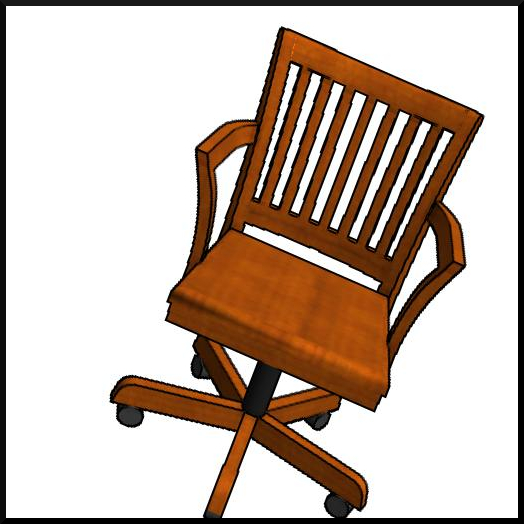
\includegraphics[scale=0.7]{imgs/data_augmentation/pic_0_1978.jpeg} }}
    \qquad
    \subfloat{{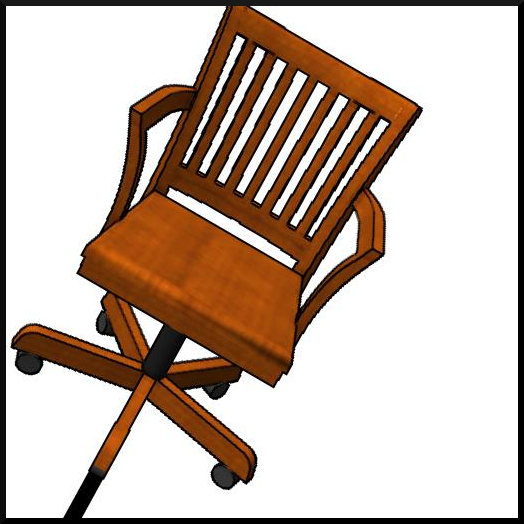
\includegraphics[scale=0.7]{imgs/data_augmentation/pic_0_2315.jpeg} }}
    \qquad
    \subfloat{{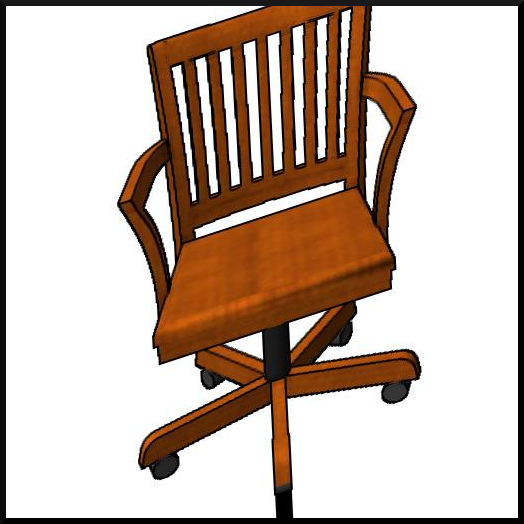
\includegraphics[scale=0.7]{imgs/data_augmentation/pic_0_3706.jpeg} }}
    \qquad
    \subfloat{{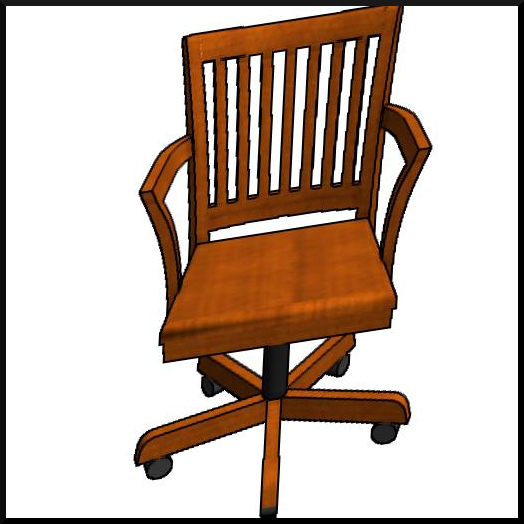
\includegraphics[scale=0.7]{imgs/data_augmentation/pic_0_7511.jpeg} }}
    \caption{Data augmentation results}
\end{figure}
When performing data augmentation, it is important to keep in mind that \textit{"Data warping augmentations transform existing images such that their label is preserved"} \cite{imagedataaugmentationsurvey}.
\begin{lstlisting}[language=Python,frame=single]
# experiment model layers
layers = [
    Conv2D(32, (3, 3), 'relu', (128, 128, 3)),
    MaxPooling2D((2, 2)),
    Conv2D(64, (3, 3), 'relu'),
    MaxPooling2D((2, 2)),
    Conv2D(128, (3, 3), 'relu'),
    MaxPooling2D((2, 2)),
    Flatten(),
    Dense(64, 'relu'),
    Dropout(0.4),
    Dense(NUM_CLASSES, 'softmax')
]

# train, validate and test
images_kfold_validation_layers(model_name="Experiment-3", n_splits=6,
    test_size=0.01, shuffle=True, layers=layers, learning_rate=0.001,
    decay=1e-6, target_size=TARGET_SIZE, epochs=100, batch_size=32,
    one_fold=True, resample_data=0, augment=True)
\end{lstlisting}
After training for $100$ epochs the results are shown in the following plots:
\begin{figure}[H]
    \centering
    \subfloat[\centering Loss]{{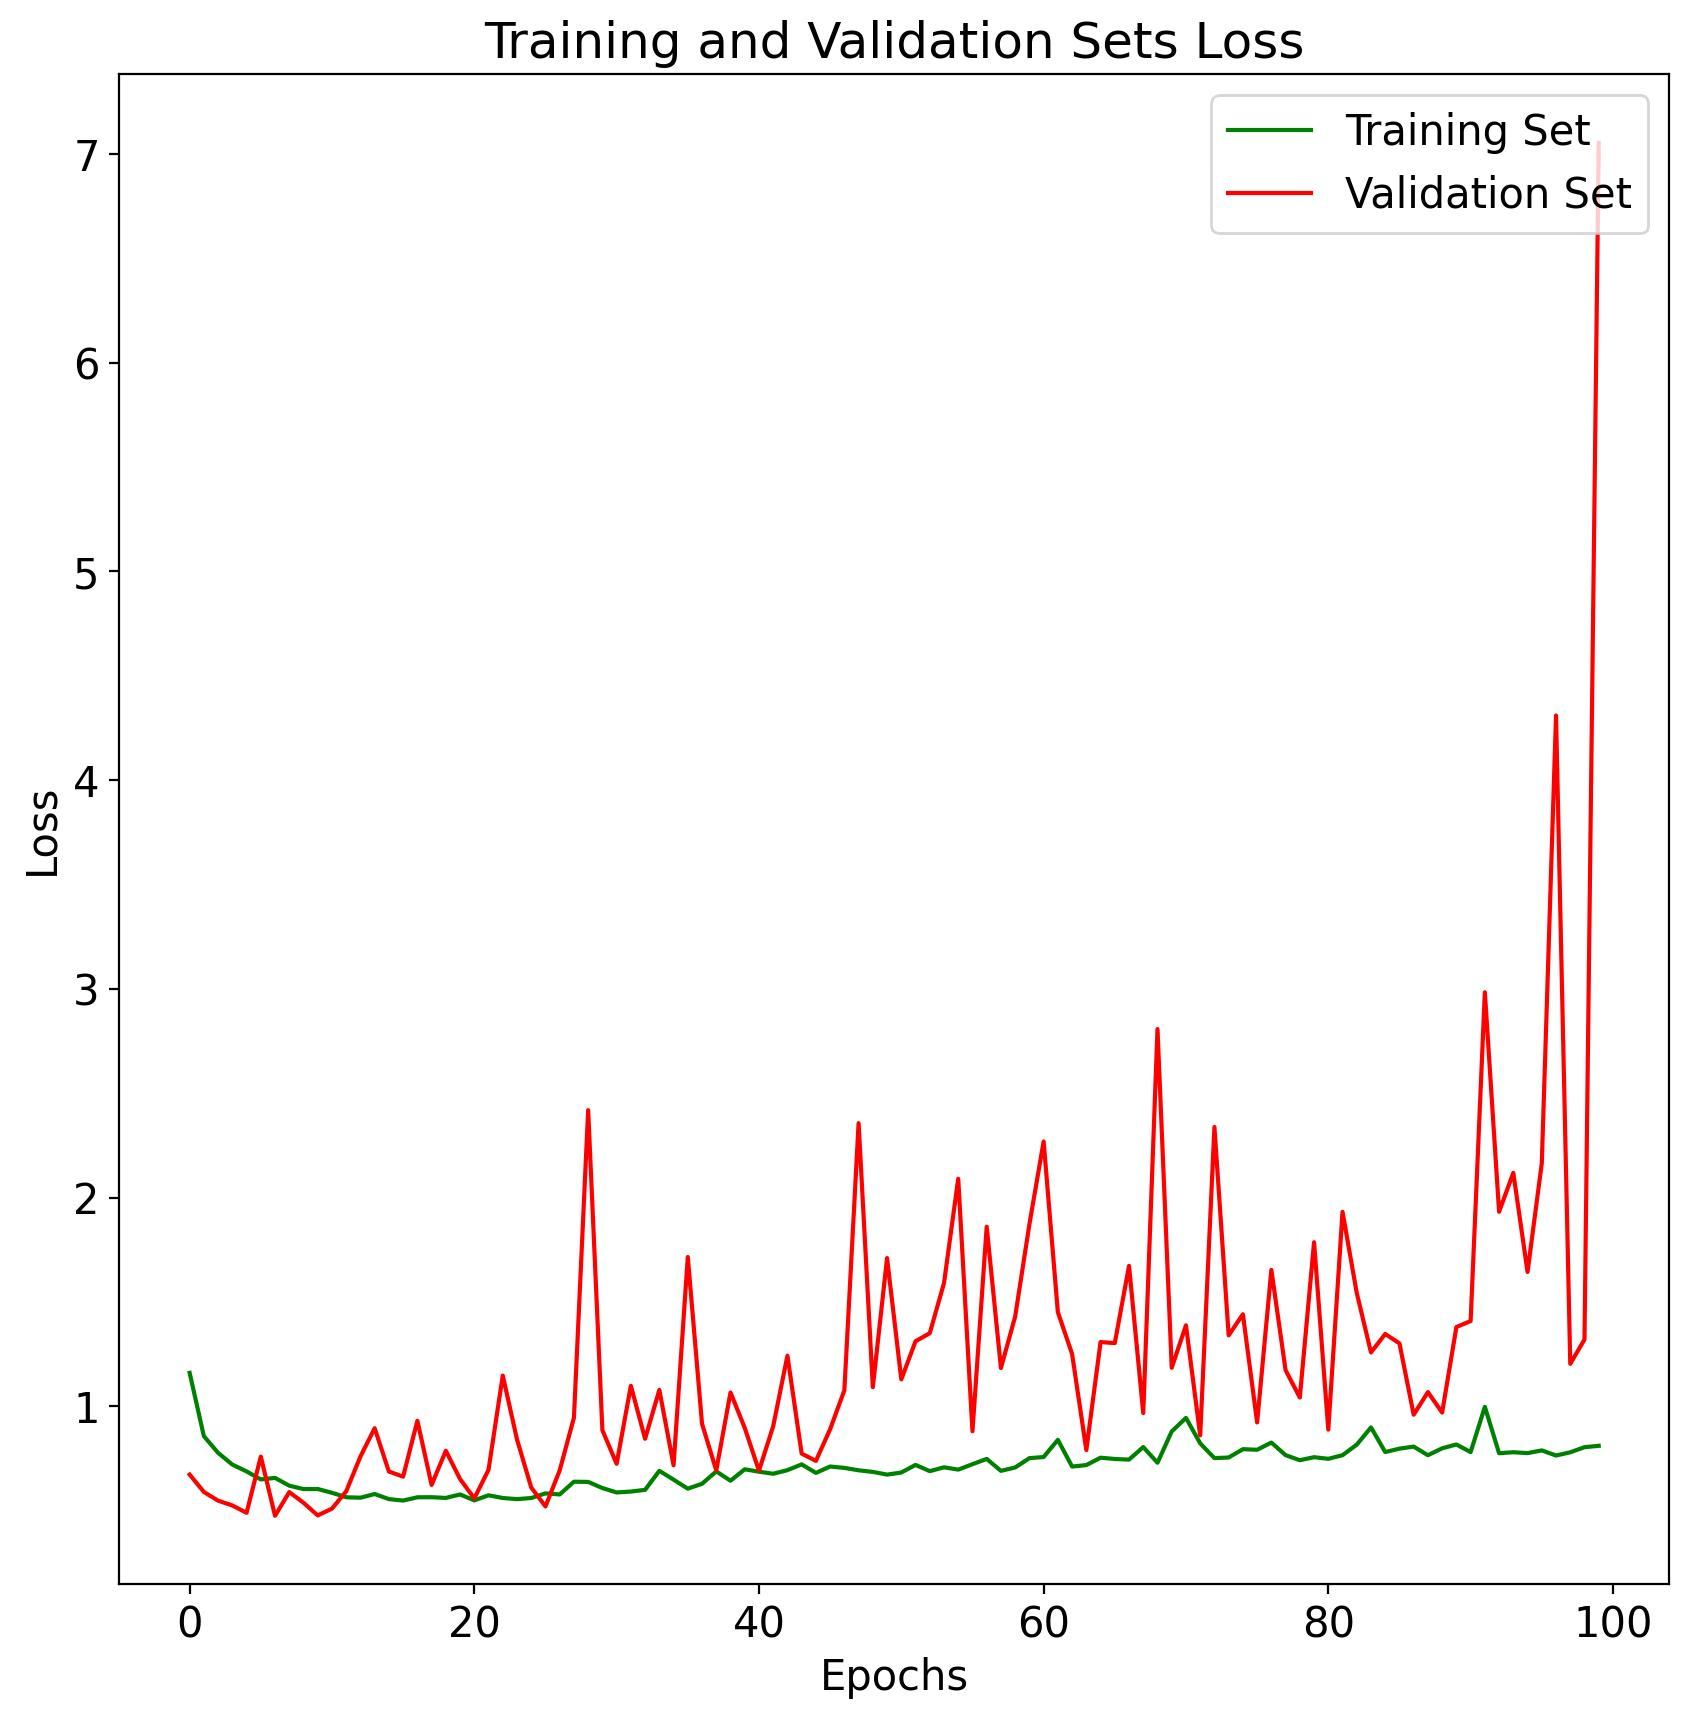
\includegraphics[scale=0.31]{imgs/experiments/images/3/Experiment-3-fold-1.h5-train-val-loss.jpg} }}
    \qquad
    \subfloat[\centering Accuracy]{{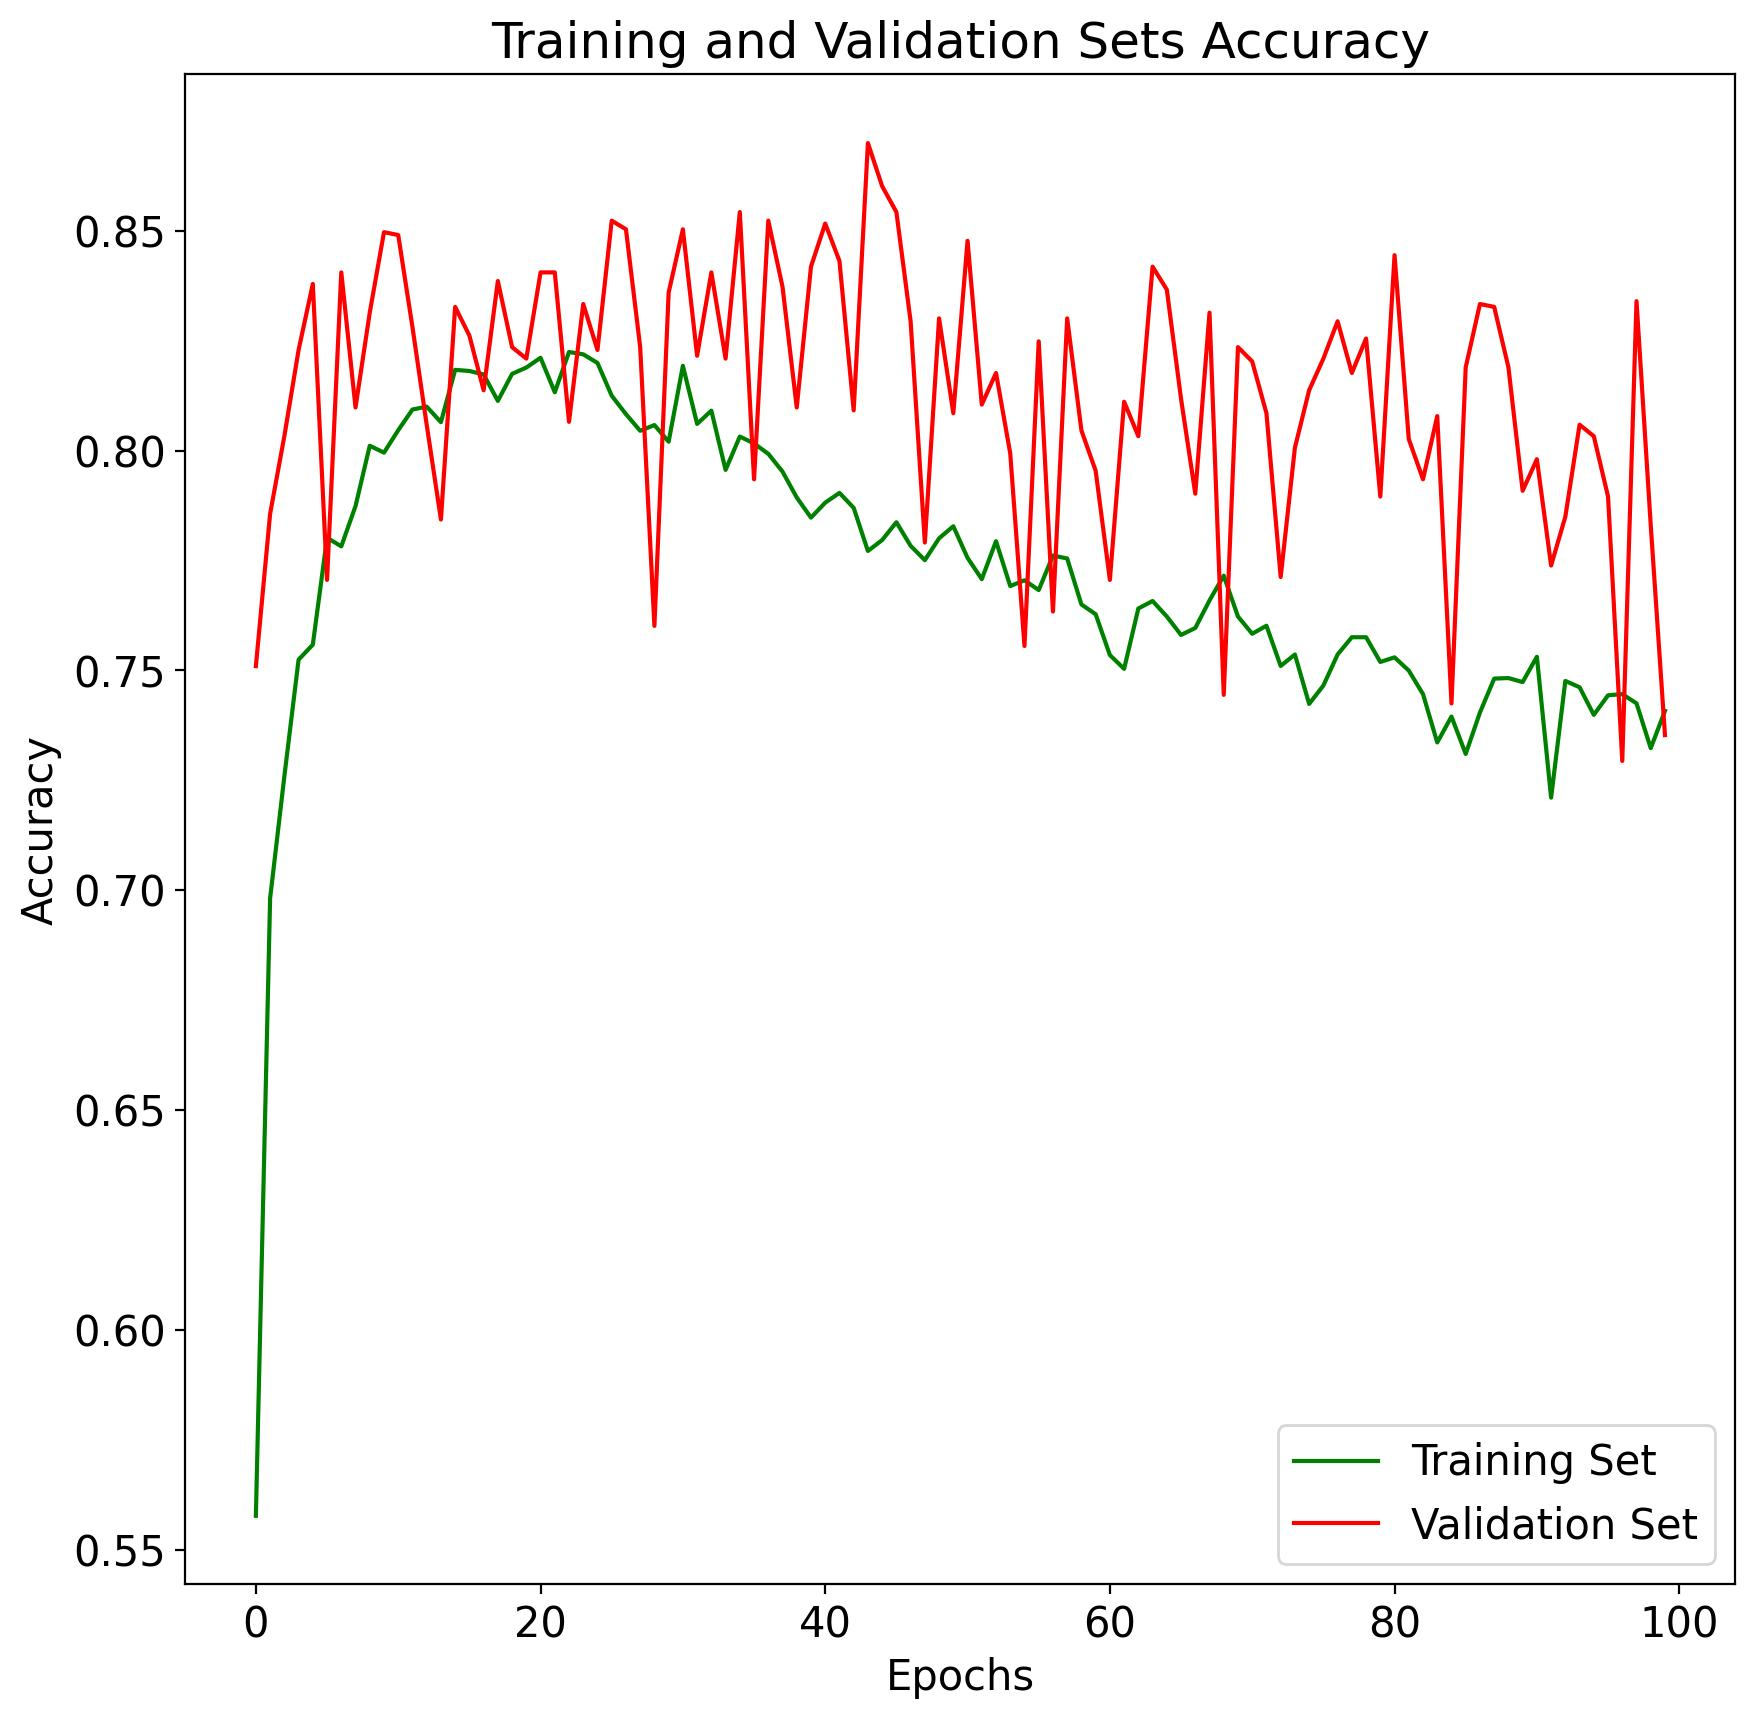
\includegraphics[scale=0.31]{imgs/experiments/images/3/Experiment-3-fold-1.h5-train-val-accuracy.jpg} }}
    \caption{Experiment 3 Results}
\end{figure}
\begin{center}
\begin{tabular}{|p{1.2cm}|p{1.8cm}|p{2cm}|p{2cm}|p{2cm}|p{2cm}|p{2cm}|}
\rowcolor{gray!50}
\hline
\textbf{Epoch} & \textbf{Training Loss} & \textbf{Training Accuracy} & \textbf{Validation Loss} & \textbf{Validation Accuracy}\\
\hline
$7$ & $0.6575$ & $0.7782$ & $0.4758$ & $0.8405$\\
\hline
\end{tabular}\\
\end{center}
Some of the conclusions we can draw from this experiment, include:
\begin{itemize}
    \item it is now safe to say that overfitting was mitigated heavily;
    \item it appears, similarly to what we experienced in the previous example, that the accuracy on the training set tends to decrease with the increase of training epochs; this must be investigated in the next experiments;
    \item overall accuracy on train and validation sets decreased due to the combined effect of dropout and data augmentation;
    \item the accuracy spikes on the validation set are actually higher since in this case the dropout layer is disabled;
\end{itemize}
\subsection{Experiment 4 - Deeper CNN, Longer Training}
In this experiment the focus was mainly on:
\begin{itemize}
    \item increasing overall accuracy by increasing the capacity of the network;
    \item increasing training epochs in order to find out if the decrease in \texttt{accuracy} on the training set is still present;
\end{itemize}
\begin{lstlisting}[language=Python,frame=single]
# experiment model layers
layers = [
    Conv2D(32, (3, 3), 'relu', (128, 128, 3)),
    MaxPooling2D((2, 2)),
    Conv2D(64, (3, 3), 'relu'),
    MaxPooling2D((2, 2)),
    Conv2D(128, (3, 3), 'relu'),
    MaxPooling2D((2, 2)),
    Conv2D(256, (3, 3), 'relu'),
    MaxPooling2D((2, 2)),
    Flatten(),
    Dense(64, 'relu'),
    Dropout(0.4),
    Dense(NUM_CLASSES, 'softmax')
]

# train, validate and test
images_kfold_validation_layers(model_name="Experiment-4", n_splits=6,
    test_size=0.01, shuffle=True, layers=layers, learning_rate=0.001,
    decay=1e-6, target_size=TARGET_SIZE, epochs=150, batch_size=32,
    one_fold=True, resample_data=0, augment=True)
\end{lstlisting}
This is the first model trained for $150$ epochs.
\begin{figure}[H]
    \centering
    \subfloat[\centering Loss]{{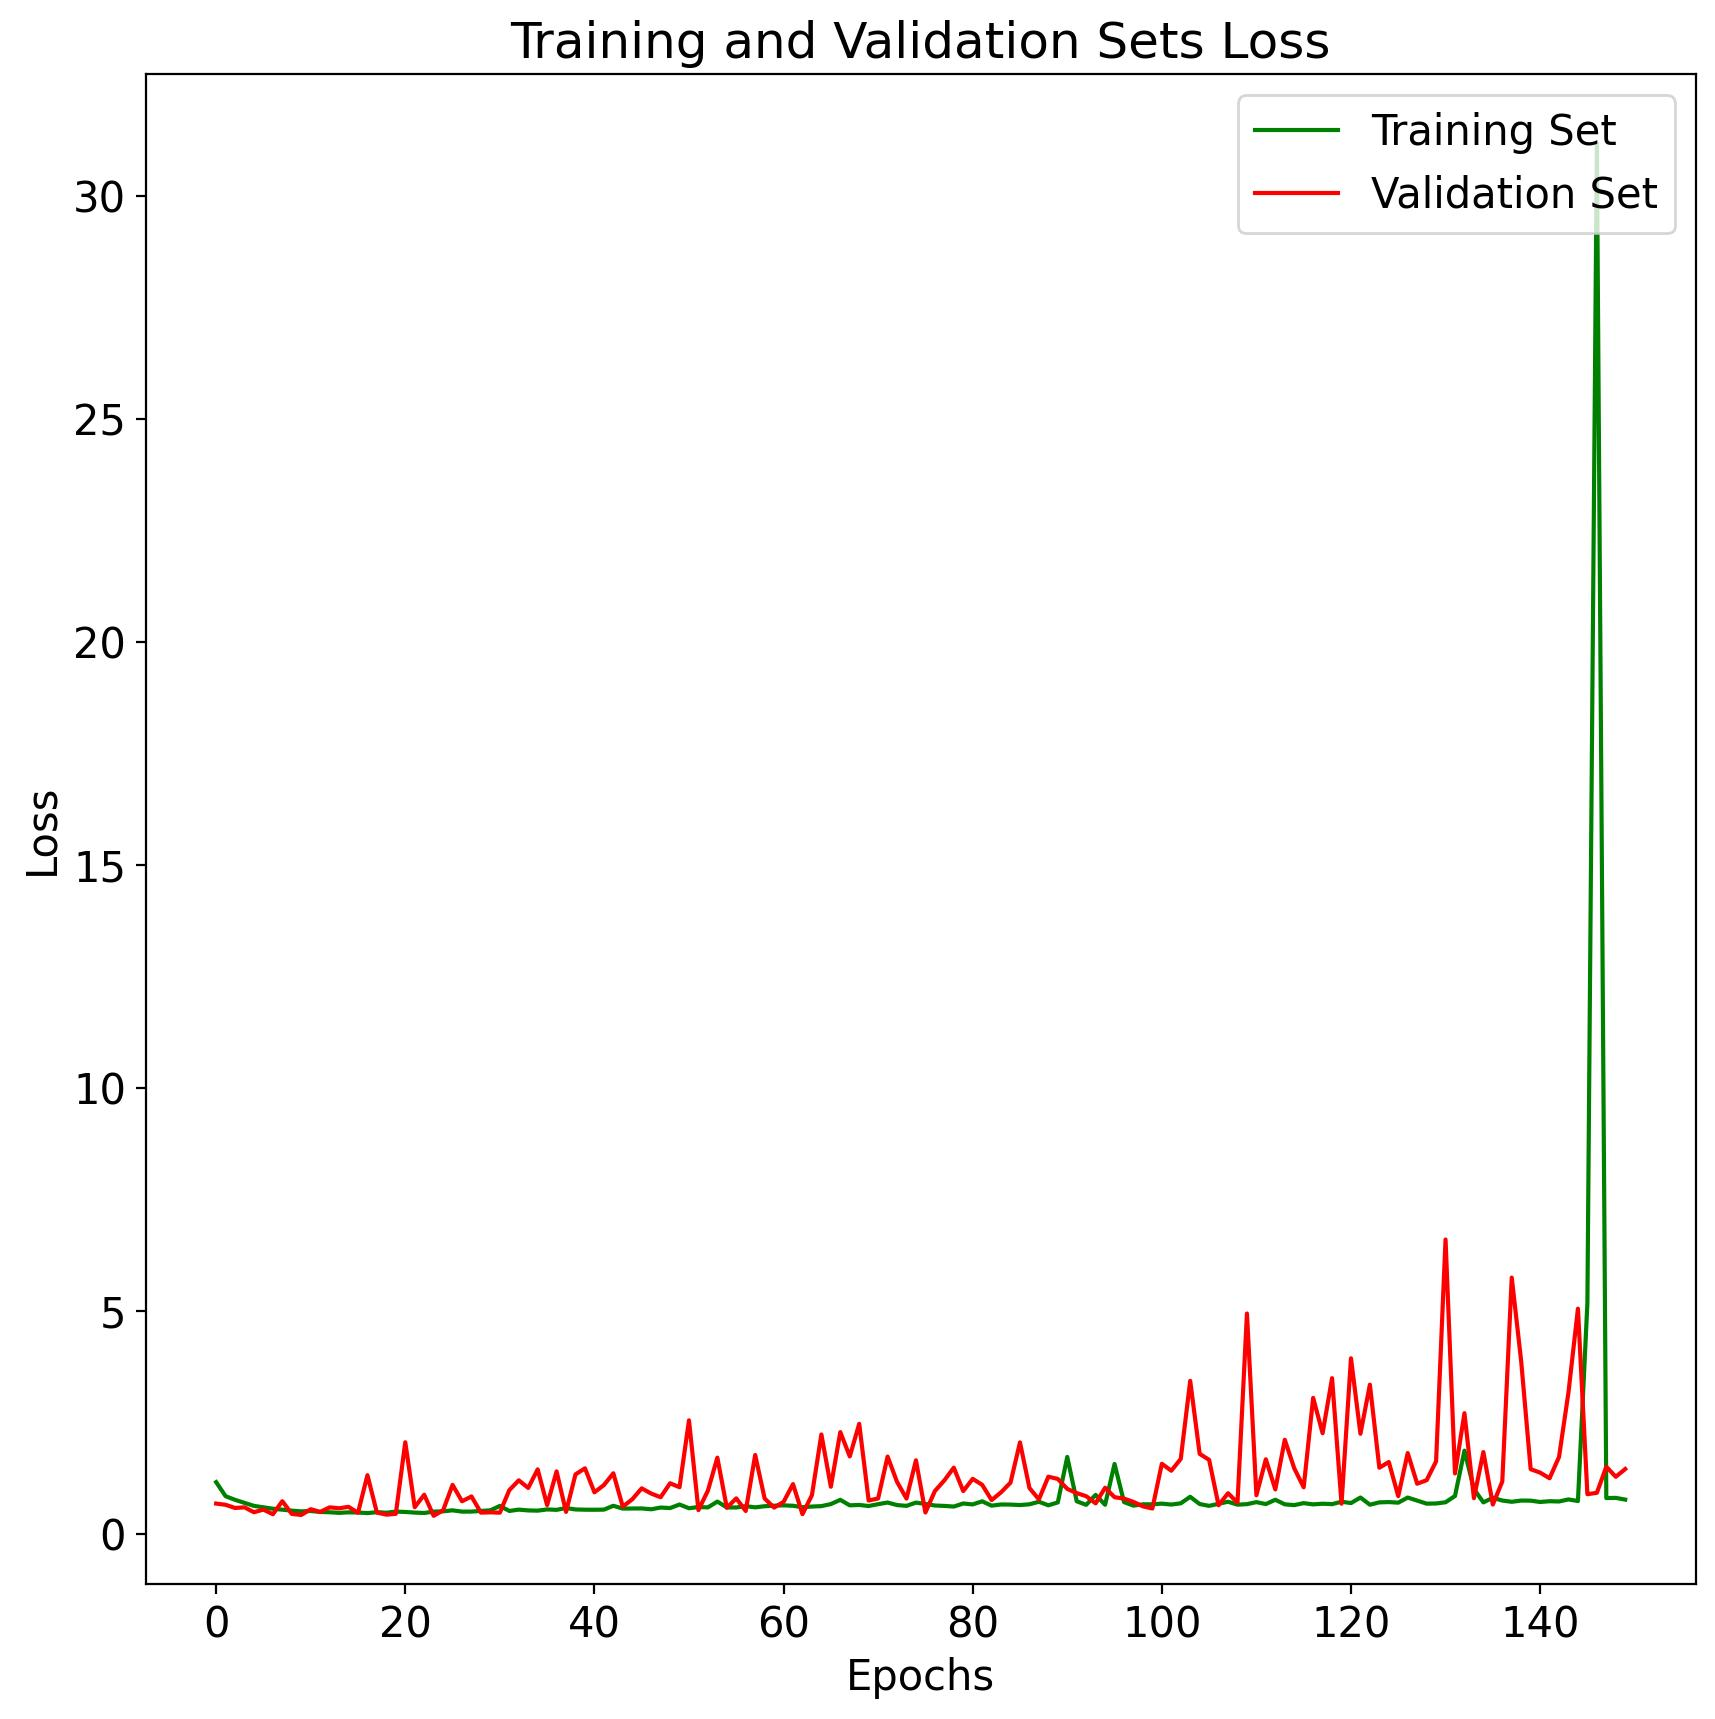
\includegraphics[scale=0.31]{imgs/experiments/images/4/Experiment-4-fold-1.h5-train-val-loss.jpg} }}
    \qquad
    \subfloat[\centering Accuracy]{{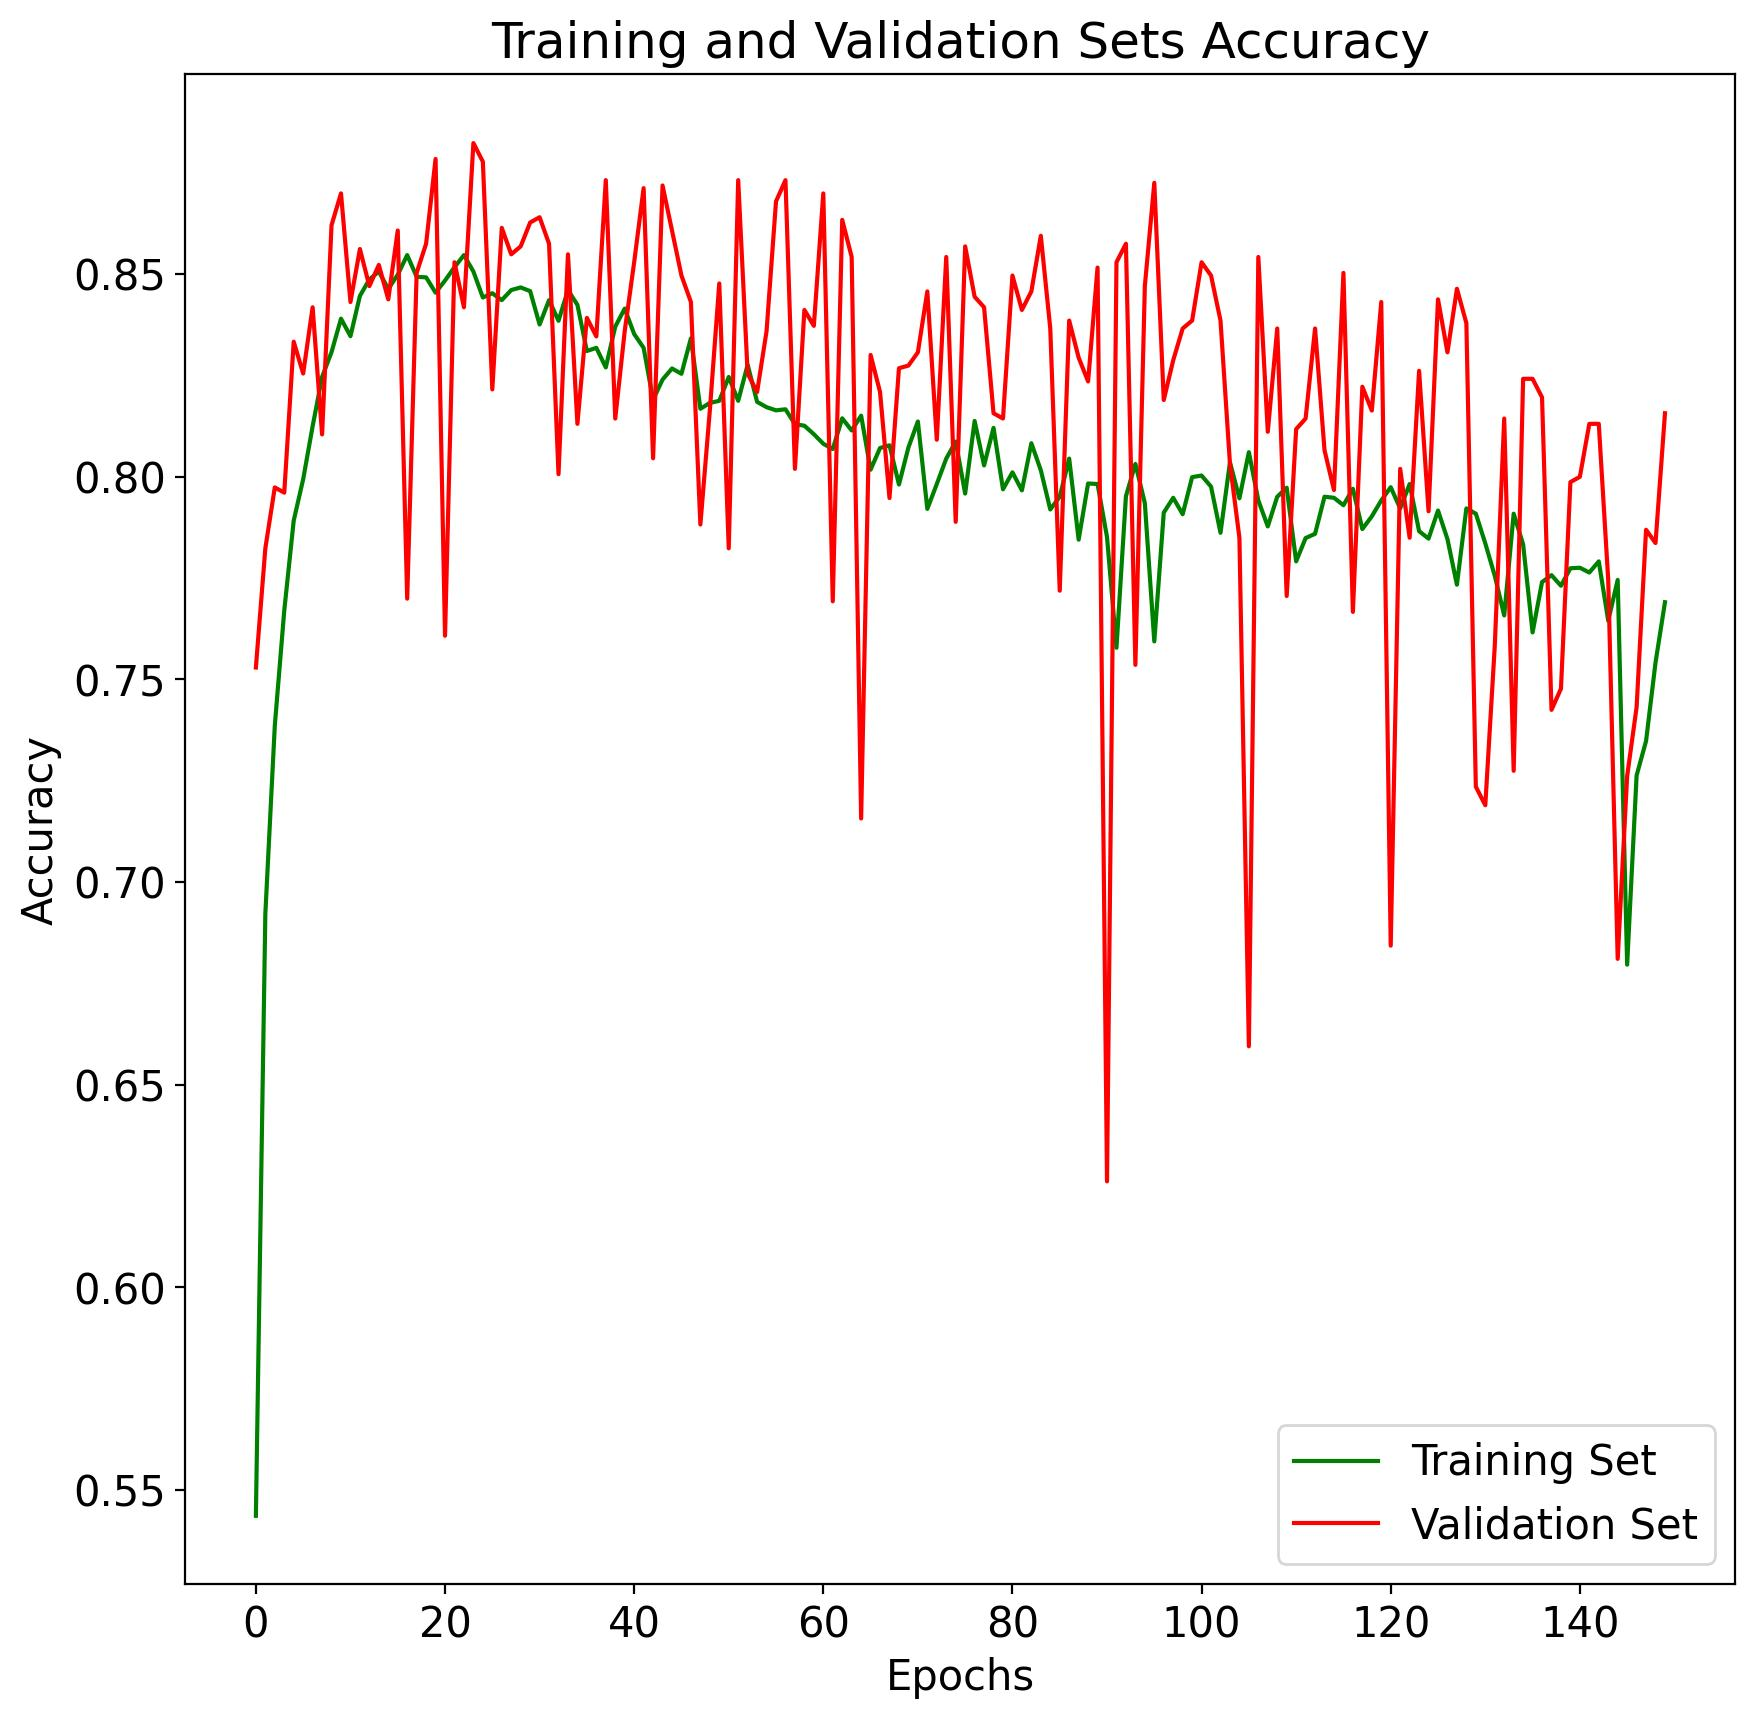
\includegraphics[scale=0.31]{imgs/experiments/images/4/Experiment-4-fold-1.h5-train-val-accuracy.jpg} }}
    \caption{Experiment 4 Results}
\end{figure}
\begin{center}
\begin{tabular}{|p{1.2cm}|p{1.8cm}|p{2cm}|p{2cm}|p{2cm}|p{2cm}|p{2cm}|}
\rowcolor{gray!50}
\hline
\textbf{Epoch} & \textbf{Training Loss} & \textbf{Training Accuracy} & \textbf{Validation Loss} & \textbf{Validation Accuracy}\\
\hline
$24$ & $0.4927$ & $0.8507$ & $0.3993$ & $0.8824$\\
\hline
\end{tabular}\\
\end{center}
Unfortunately a spike happened in the Loss plot which makes it difficult to understand. However, from the plot of the accuracy, what worries me most is that the accuracy curve has a negative inclination and that the overall accuracy does not stabilize around $85\%$. In addition, the noise on the validation set is extremely high. These points gave the basis for the next experiment.
\subsection{Experiment 5 - Larger Dense Layer, Larger Batch Size}
In this experiment the focus was mainly on:
\begin{itemize}
    \item the optimization process in the two previous experiments is still quite noisy, which could be a symptom of a \textbf{too small batch size}; as a result the batch size was doubled from $32$ to $64$; in theory, increasing the batch size will allow for a more precise gradient computation with reduced noise;
    \item still the accuracy on the training set is achieving scores around $83\%$; one thing worth trying is increasing the size of the fully connected dense layer found at the end of the network; this is done because most of the weights are found in this layer and it might represent a bottleneck to the learning/generalization capabilities of the network; the number of units of the \texttt{Dense} layer was doubled from $64$ to $128$;
    \item the model will be trained for $200$ epochs in order to understand what is going on with the negative inclination of the accuracy curve; \textbf{this might be related to some biases introduced as a result of data augmentation applied in Experiment 3.}
\end{itemize}
\begin{lstlisting}[language=Python,frame=single]
# experiment model layers
layers = [
    Conv2D(32, (3, 3), 'relu', (128, 128, 3)),
    MaxPooling2D((2, 2)),
    Conv2D(64, (3, 3), 'relu'),
    MaxPooling2D((2, 2)),
    Conv2D(128, (3, 3), 'relu'),
    MaxPooling2D((2, 2)),
    Conv2D(256, (3, 3), 'relu'),
    MaxPooling2D((2, 2)),
    Flatten(),
    Dense(128, 'relu'),
    Dropout(0.4),
    Dense(NUM_CLASSES, 'softmax')
]

# train, validate and test
images_kfold_validation_layers(model_name="Experiment-5", n_splits=6,
    test_size=0.01, shuffle=True, layers=layers, learning_rate=0.001,
    decay=1e-6, target_size=TARGET_SIZE, epochs=200, batch_size=64,
    one_fold=True, resample_data=0, augment=True)
\end{lstlisting}
After $200$ epochs of training, the results achieved are the best ever since the beginning of the trial and error process. Additionally, we can now conclude that the decrease in accuracy does not continue indefinitely and that the model stabilizes in the long run. Even after the increase of the \texttt{capacity} of the model, overfitting did not started reappearing again. It is also evident that the oscillations of the accuracy score on the validation set decreased as a result of using a larger batch size.
\begin{figure}[H]
    \centering
    \subfloat[\centering Loss]{{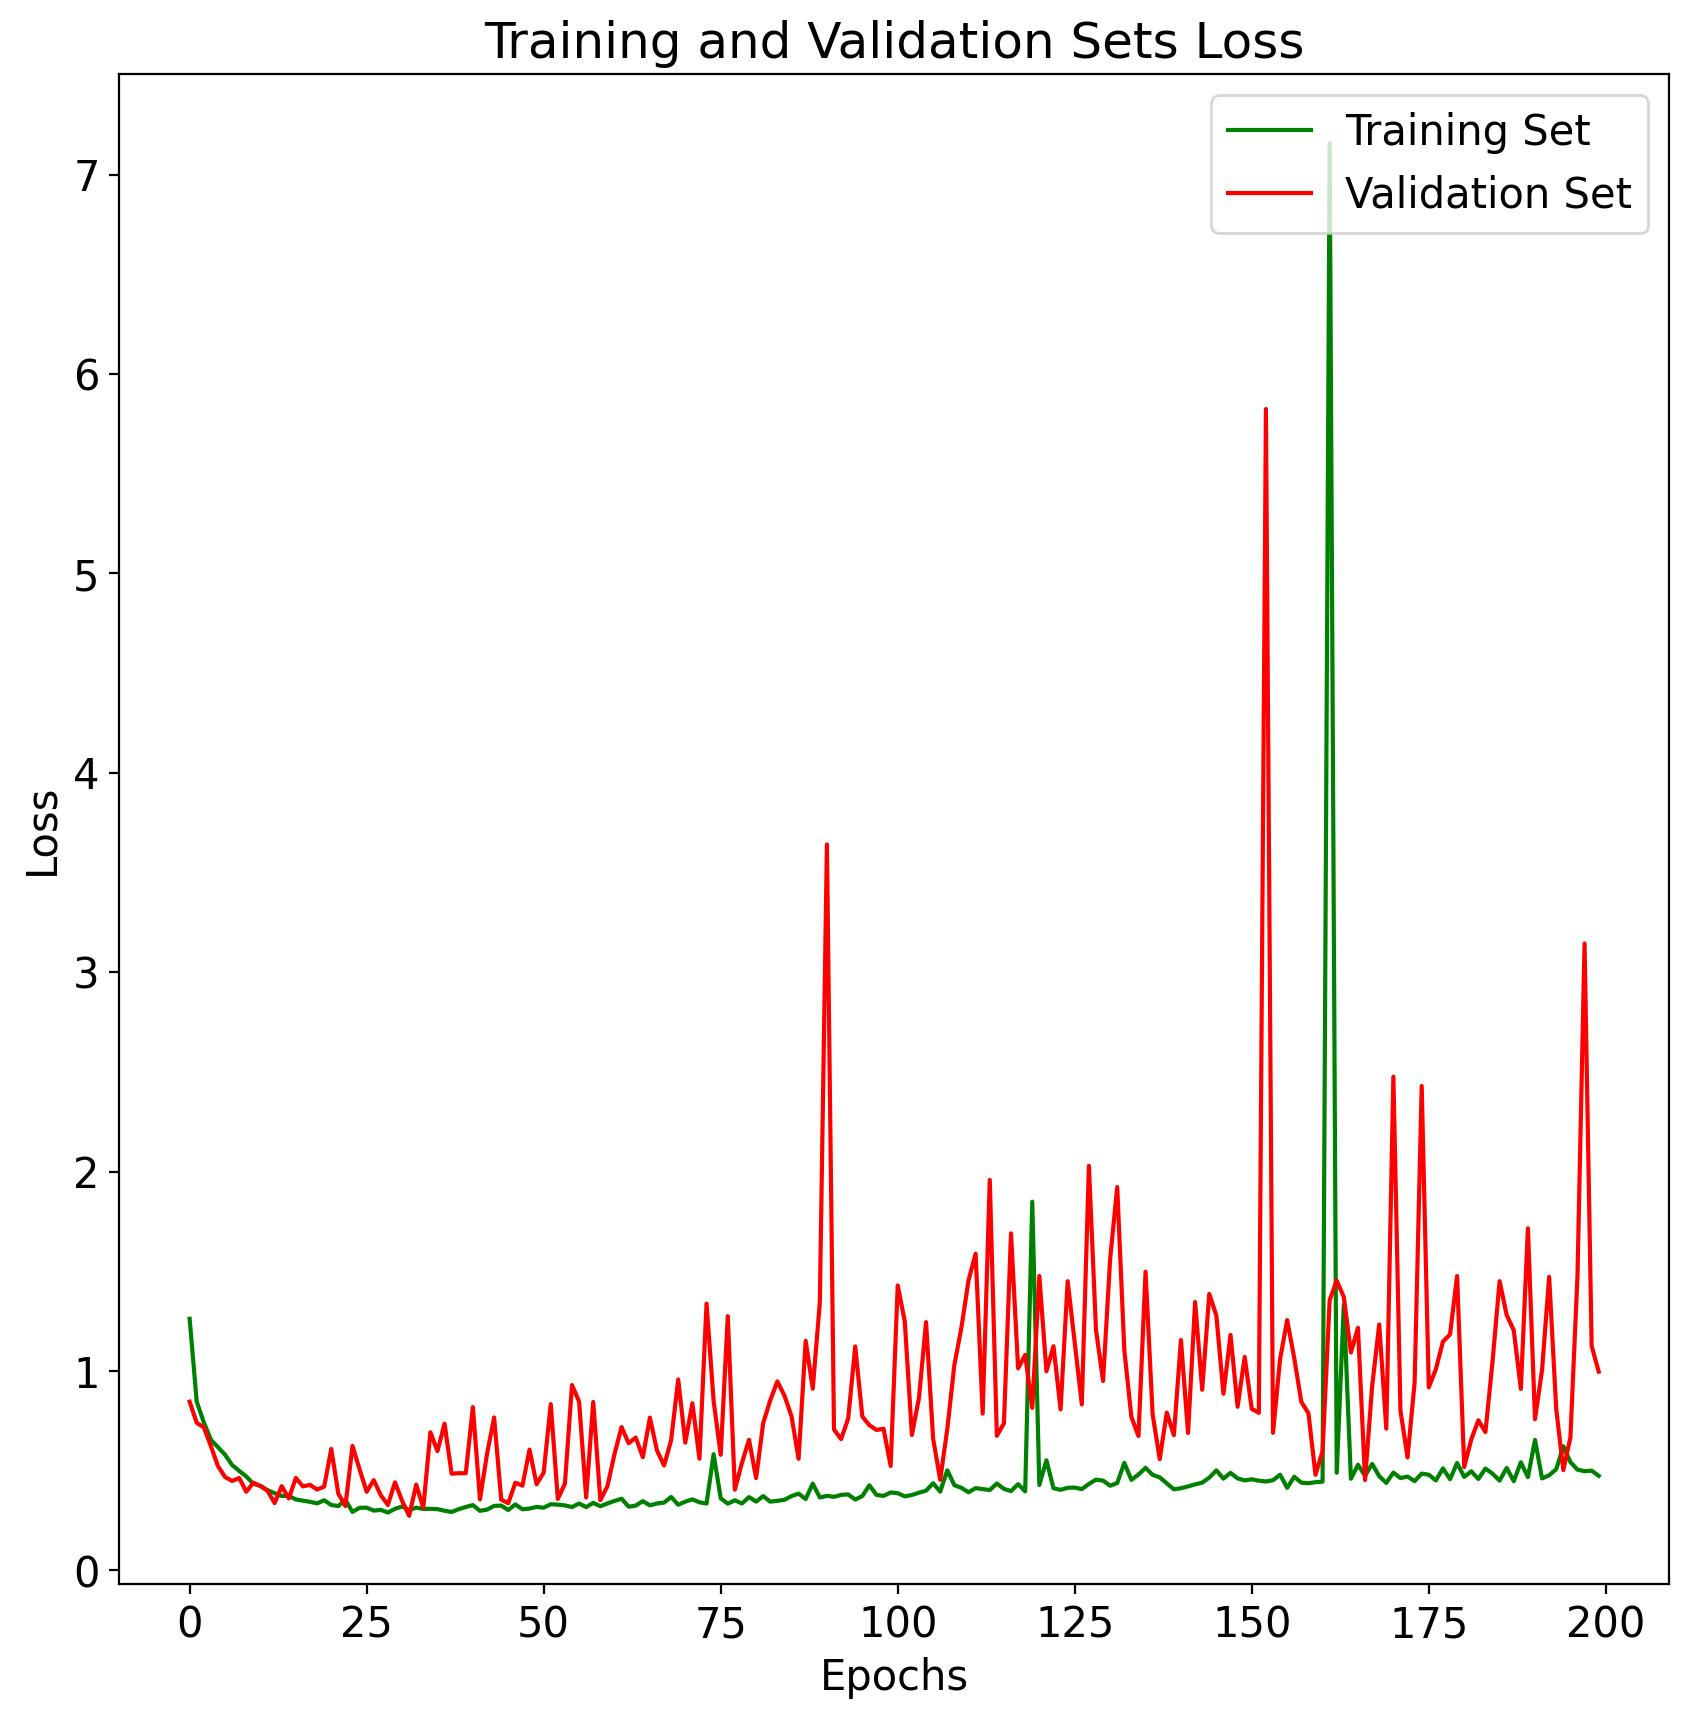
\includegraphics[scale=0.31]{imgs/experiments/images/5/Experiment-5-fold-1.h5-train-val-loss.jpg} }}
    \qquad
    \subfloat[\centering Accuracy]{{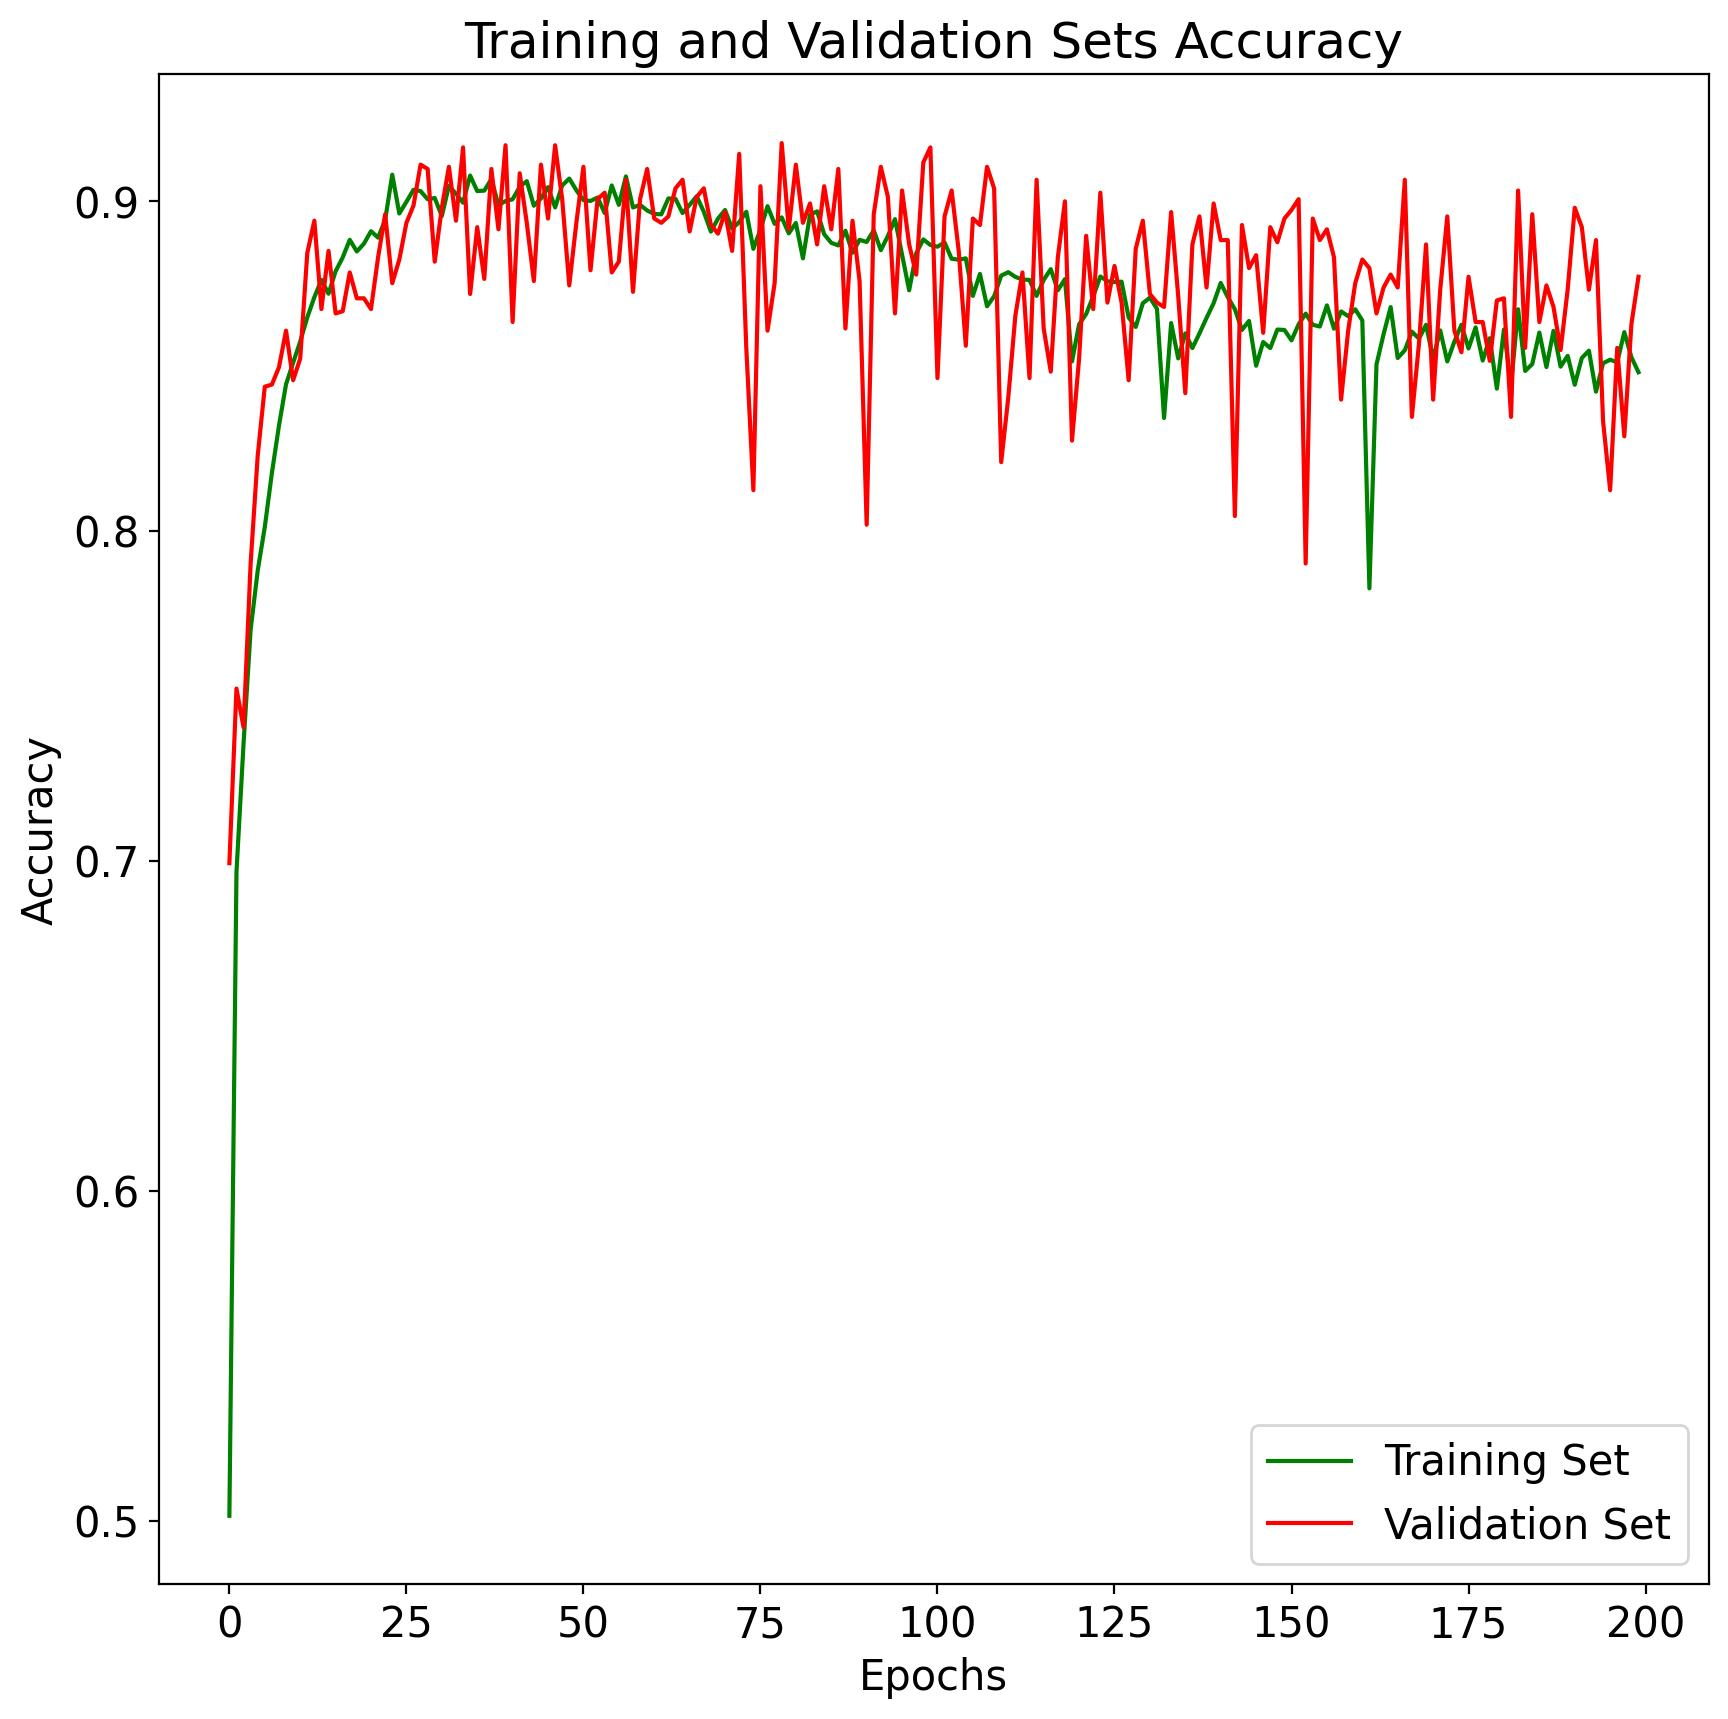
\includegraphics[scale=0.31]{imgs/experiments/images/5/Experiment-5-fold-1.h5-train-val-accuracy.jpg} }}
    \caption{Experiment 5 Results}
\end{figure}
\begin{center}
\begin{tabular}{|p{1.2cm}|p{1.8cm}|p{2cm}|p{2cm}|p{2cm}|p{2cm}|p{2cm}|}
\rowcolor{gray!50}
\hline
\textbf{Epoch} & \textbf{Training Loss} & \textbf{Training Accuracy} & \textbf{Validation Loss} & \textbf{Validation Accuracy}\\
\hline
$32$ & $0.3022$ & $0.9047$ & $0.2741$ & $0.9105$\\
\hline
\end{tabular}\\
\end{center}
My current hypothesis is that a spike in accuracy happens as a result of an initial overfitting on the training set and then accuracy gradually decreases stabilizing on the real value. In order to avoid this behavior, the learning rate decay might be of help.
\subsection{Experiment 6 - Learning Rate Decay}
This experiment can be considered a first attempt of tuning the \texttt{learning rate decay} parameter. For all the experiments performed till this point, the extremely low value of $1e-6$ was used. Given the number of epochs for which training was carried out, this basically means no decay. Learning rate decay \cite{you2019does} is a \emph{de facto} technique for training modern neural networks. It starts with a large learning rate and then decays it multiple times. It is empirically observed to help both optimization and generalization. Common beliefs in how the decay rate works come from the optimization analysis of (Stochastic) Gradient Descent:
\begin{itemize}
    \item an initially large learning rate accelerates training or helps the network escape spurious local minima;
    \item decaying the learning rate helps the network converge to a local minimum and avoid oscillation.
\end{itemize}
A step decay schedule that drops the learning rate by a factor every few epochs was implemented. The initial \texttt{learning rate} of $0.001$ is dropped by a factor of $0.9$ every $30$ epochs\footnote{Originally seen here:\\ \url{https://pyimagesearch.com/2019/07/22/keras-learning-rate-schedules-and-decay/}.}.
\begin{lstlisting}[language=Python,frame=single]
class LearningRateDecay:
    def plot(self, save_path, epochs, title="Learning Rate Schedule"):
        # compute the set of learning rates for each corresponding epoch
        lrs = [self(i) for i in epochs]

        # the learning rate schedule
        plt.style.use("ggplot")
        plt.figure(figsize=(10, 10))
        plt.plot(epochs, lrs)
        plt.title(title)
        plt.xlabel("Epochs")
        plt.ylabel("Learning Rate")
        plt.savefig(save_path + '-lr-decay.jpg', bbox_inches='tight', dpi=200)
        plt.show()

class StepDecay(LearningRateDecay):
    def __init__(self, initAlpha=0.001, factor=0.9, dropEvery=30):
        # store the base initial learning rate, drop factor, and
        # epochs to drop every
        self.initAlpha = initAlpha
        self.factor = factor
        self.dropEvery = dropEvery

    def __call__(self, epoch):
        # compute the learning rate for the current epoch
        exp = numpy.floor((1 + epoch) / self.dropEvery)
        alpha = self.initAlpha * (self.factor ** exp)

        # return the learning rate
        return float(alpha)
\end{lstlisting}
After $200$ epochs of training:
\begin{figure}[H]
    \centering
    \subfloat[\centering Loss]{{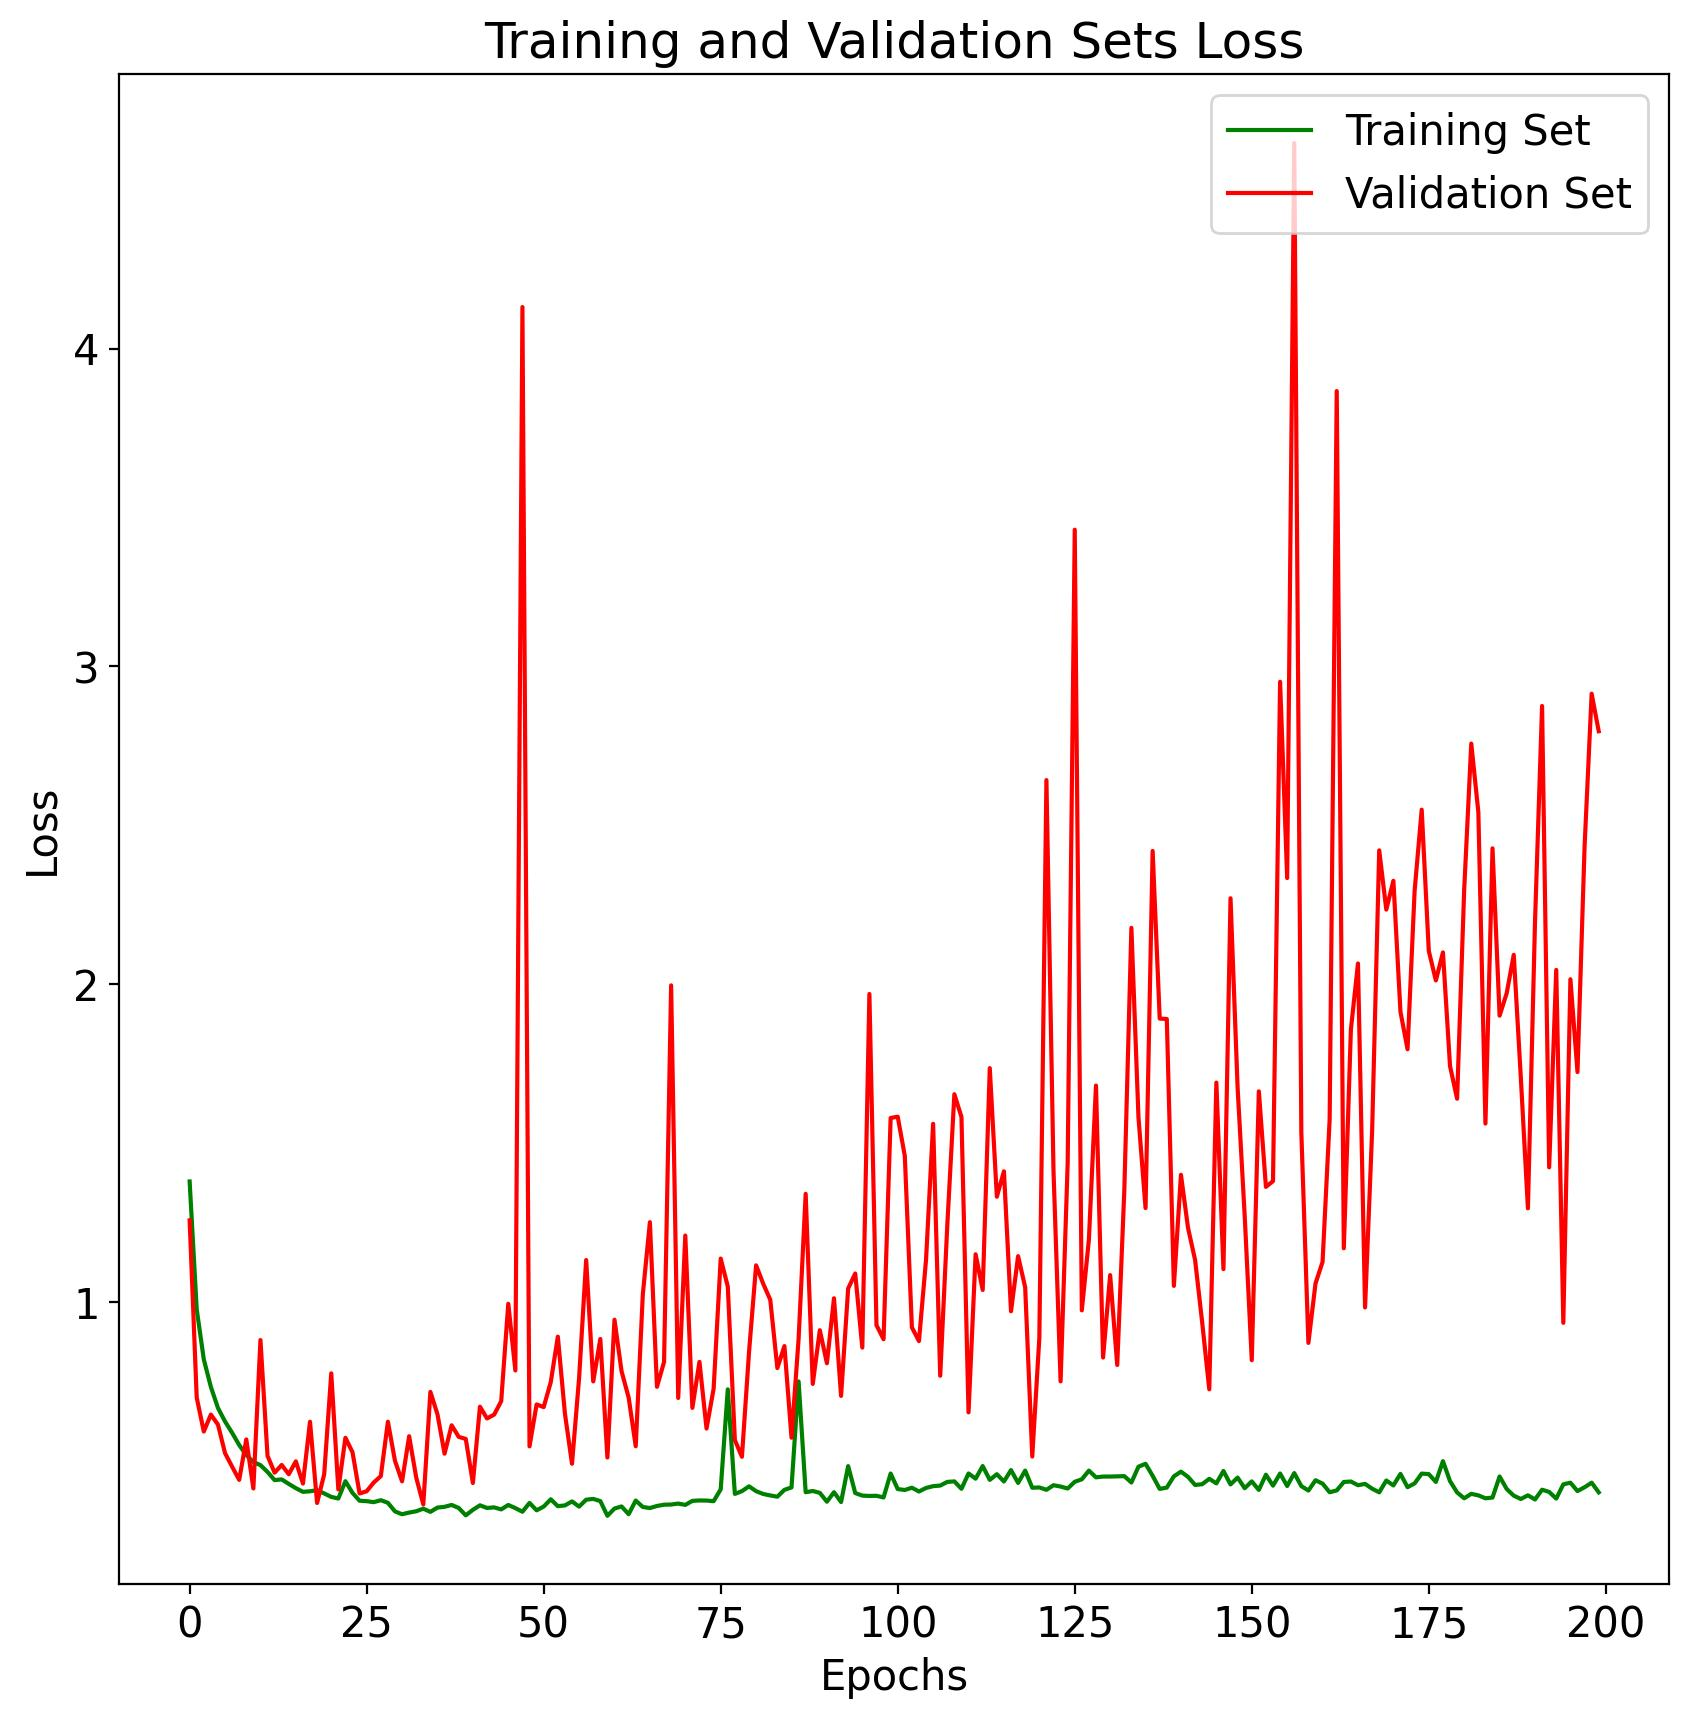
\includegraphics[scale=0.31]{imgs/experiments/images/6/Experiment-6-fold-1.h5-train-val-loss.jpg} }}
    \qquad
    \subfloat[\centering Accuracy]{{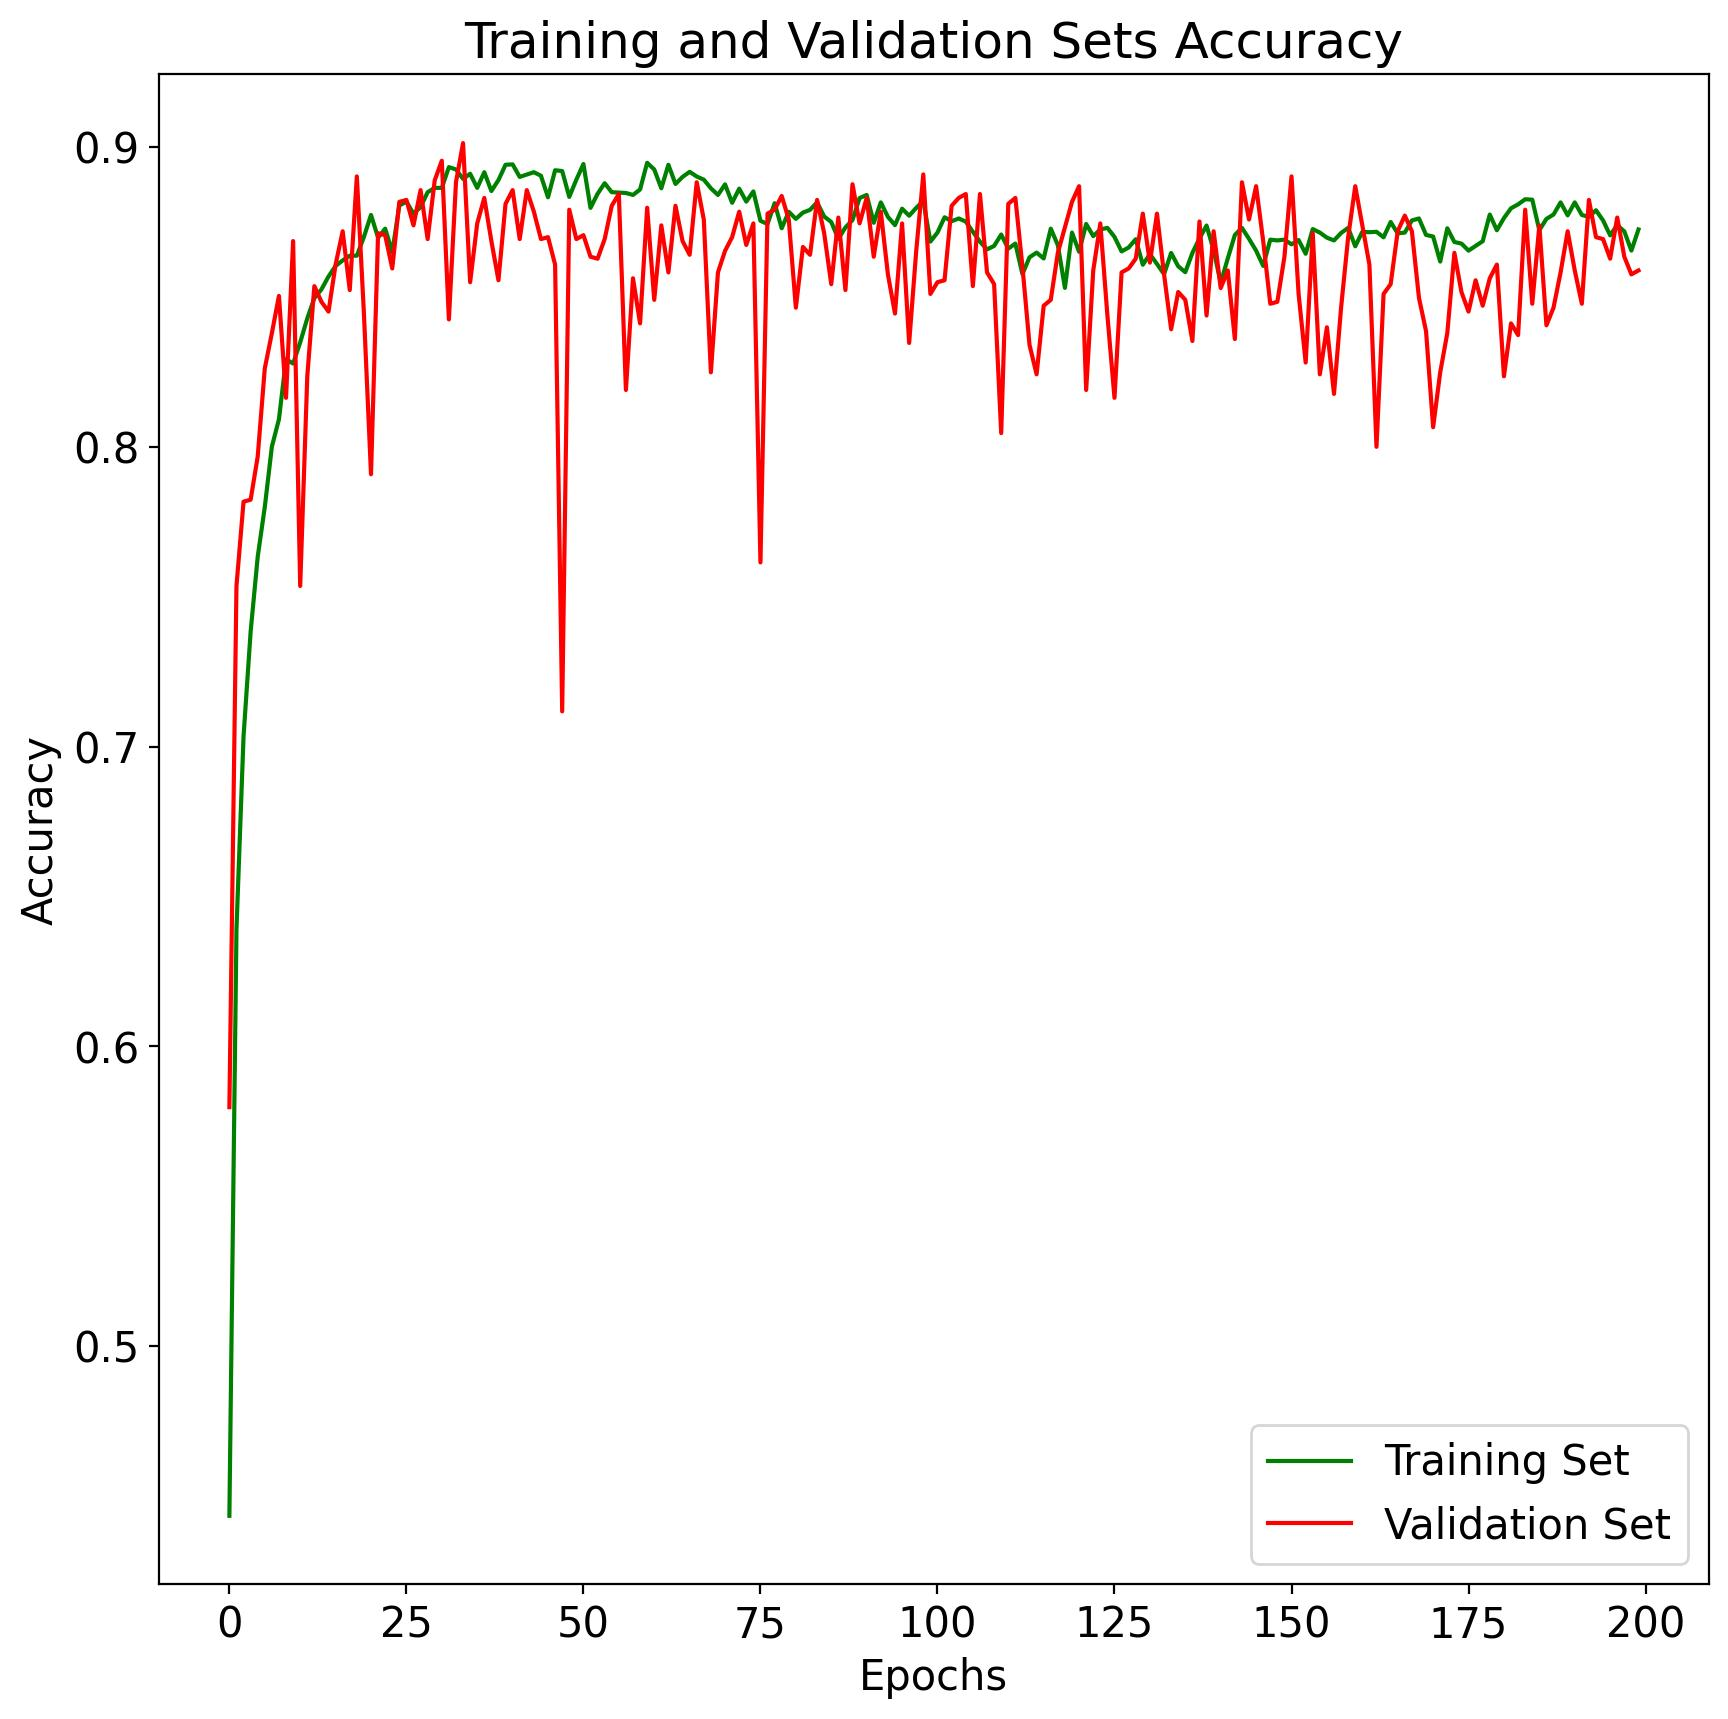
\includegraphics[scale=0.31]{imgs/experiments/images/6/Experiment-6-fold-1.h5-train-val-accuracy.jpg} }}
    \caption{Experiment 6 Results}
\end{figure}
\begin{center}
\begin{tabular}{|p{1.2cm}|p{1.8cm}|p{2cm}|p{2cm}|p{2cm}|p{2cm}|p{2cm}|}
\rowcolor{gray!50}
\hline
\textbf{Epoch} & \textbf{Training Loss} & \textbf{Training Accuracy} & \textbf{Validation Loss} & \textbf{Validation Accuracy}\\
\hline
$34$ & $0.3497$ & $0.8894$ & $0.3631$ & $0.9013$\\
\hline
\end{tabular}\\
\end{center}
\texttt{tf.keras.callbacks.LearningRateScheduler} was used in order to plot the learning schedule values epoch after epoch:
\begin{figure}[H]
    \centering
    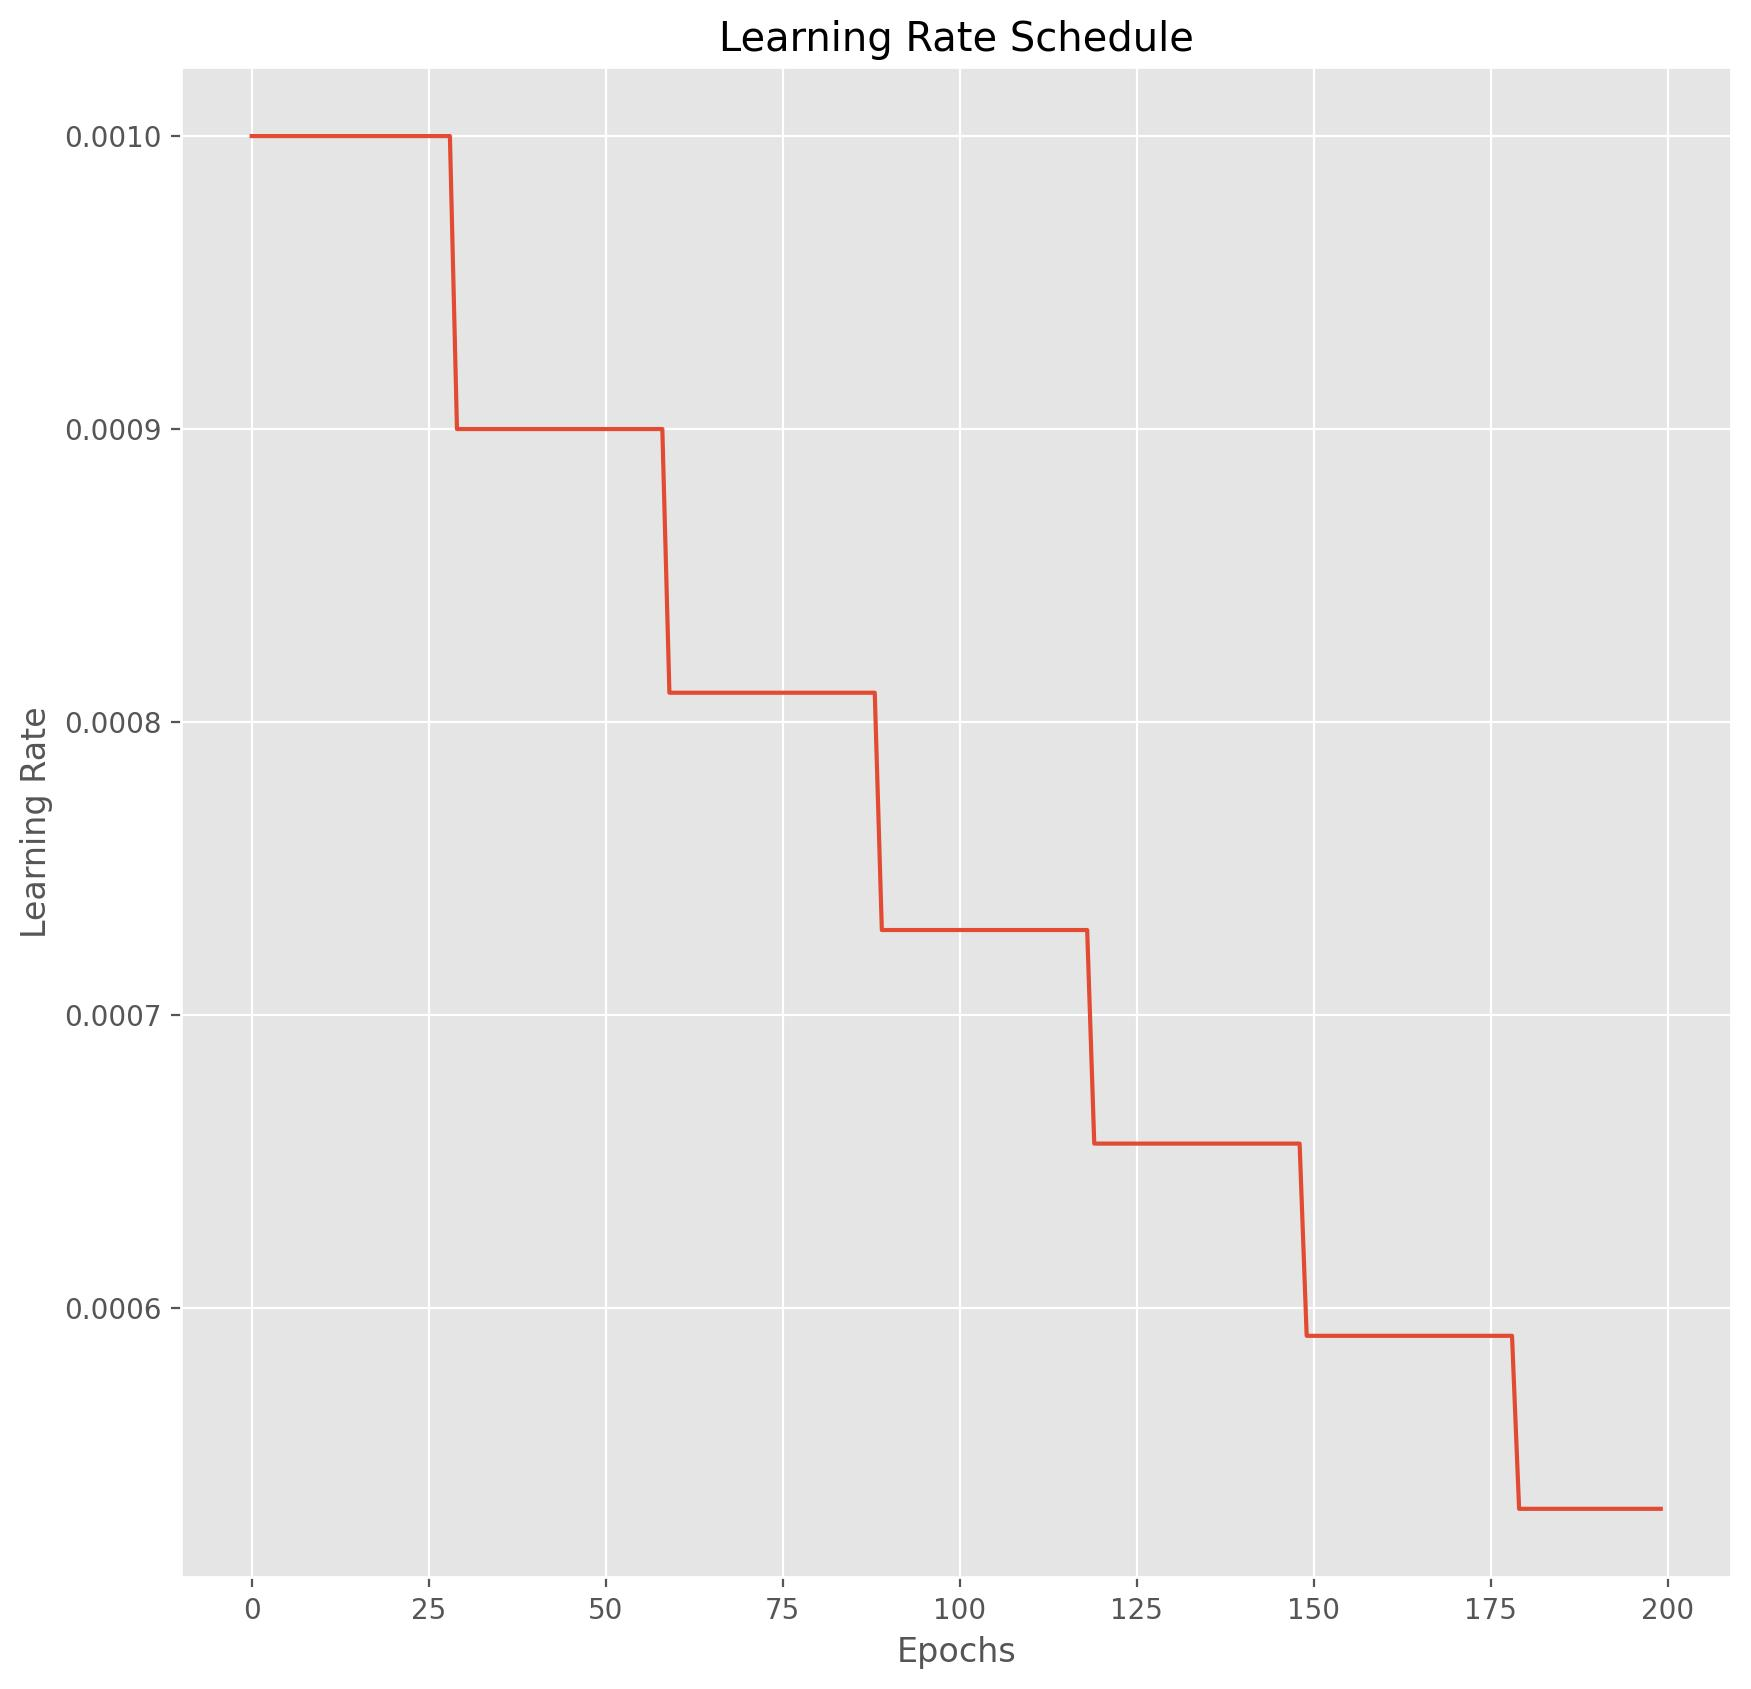
\includegraphics[scale=0.5]{imgs/experiments/images/6/Experiment-6-fold-1.h5-lr-decay.jpg}
\end{figure}
\noindent
As a result of using learning rate decay, needless to say, the learning process is much smoother and oscillation are almost completely gone. Overfitting is not affecting the learning process and almost $91\%$ of accuracy was achieved on the validation set.
\subsection{Experiment 7 - Larger Kernel, Early Stopping}
In the plot of the previous experiment, if we focus on the \texttt{accuracy} plot then overfitting is not visible; however, on the \texttt{loss} plot we can spot a deviation between the scores on the training set and the ones on the validation set. Instead of using an additional regularization technique, I decided to increase the size of the Kernel of the first two convolutional layers of the model. This was done based on the reasoning that a smaller kernel size might not be able to capture bigger features \cite{8742484}. This is only an assumption.\\
\\
Given the increase of the capacity of the network and the increase of the batch size, which can be considered an alternative to decreasing the learning rate, it takes more time to train the model also because of the high number of samples in the dataset. Too many epochs can lead to overfitting of the training dataset, whereas too few may result in an underfit model. Early Stopping is a regularization technique for deep neural networks that stops training when parameter updates no longer begin to yield improves on a validation set. As a result, \texttt{callbacks.EarlyStopping} was used in order to allow for the network to train for an arbitrarily long number of epochs and stop if there is no improvement ($0.1\%$) in the \texttt{validation accuracy} score for more than $100$ epochs.
\begin{lstlisting}[language=Python,frame=single]
# experiment model layers
layers = [
    Conv2D(32, (5, 5), 'relu', (128, 128, 3)),
    MaxPooling2D((2, 2)),
    Conv2D(64, (4, 4), 'relu'),
    MaxPooling2D((2, 2)),
    Conv2D(128, (3, 3), 'relu'),
    MaxPooling2D((2, 2)),
    Conv2D(256, (3, 3), 'relu'),
    MaxPooling2D((2, 2)),
    Flatten(),
    Dense(128, 'relu'),
    Dropout(0.4),
    Dense(NUM_CLASSES, 'softmax')
]

# train, validate and test
images_kfold_validation_layers(model_name="Experiment-7", n_splits=6,
    test_size=0.01, shuffle=True, layers=layers, learning_rate=0.001,
    decay=1e-6, target_size=TARGET_SIZE, epochs=300, batch_size=64,
    one_fold=True, resample_data=0, augment=True)
\end{lstlisting}
Thanks to \texttt{early stopping}, the training lasted only $132$ epochs.
\begin{figure}[H]
    \centering
    \subfloat[\centering Loss]{{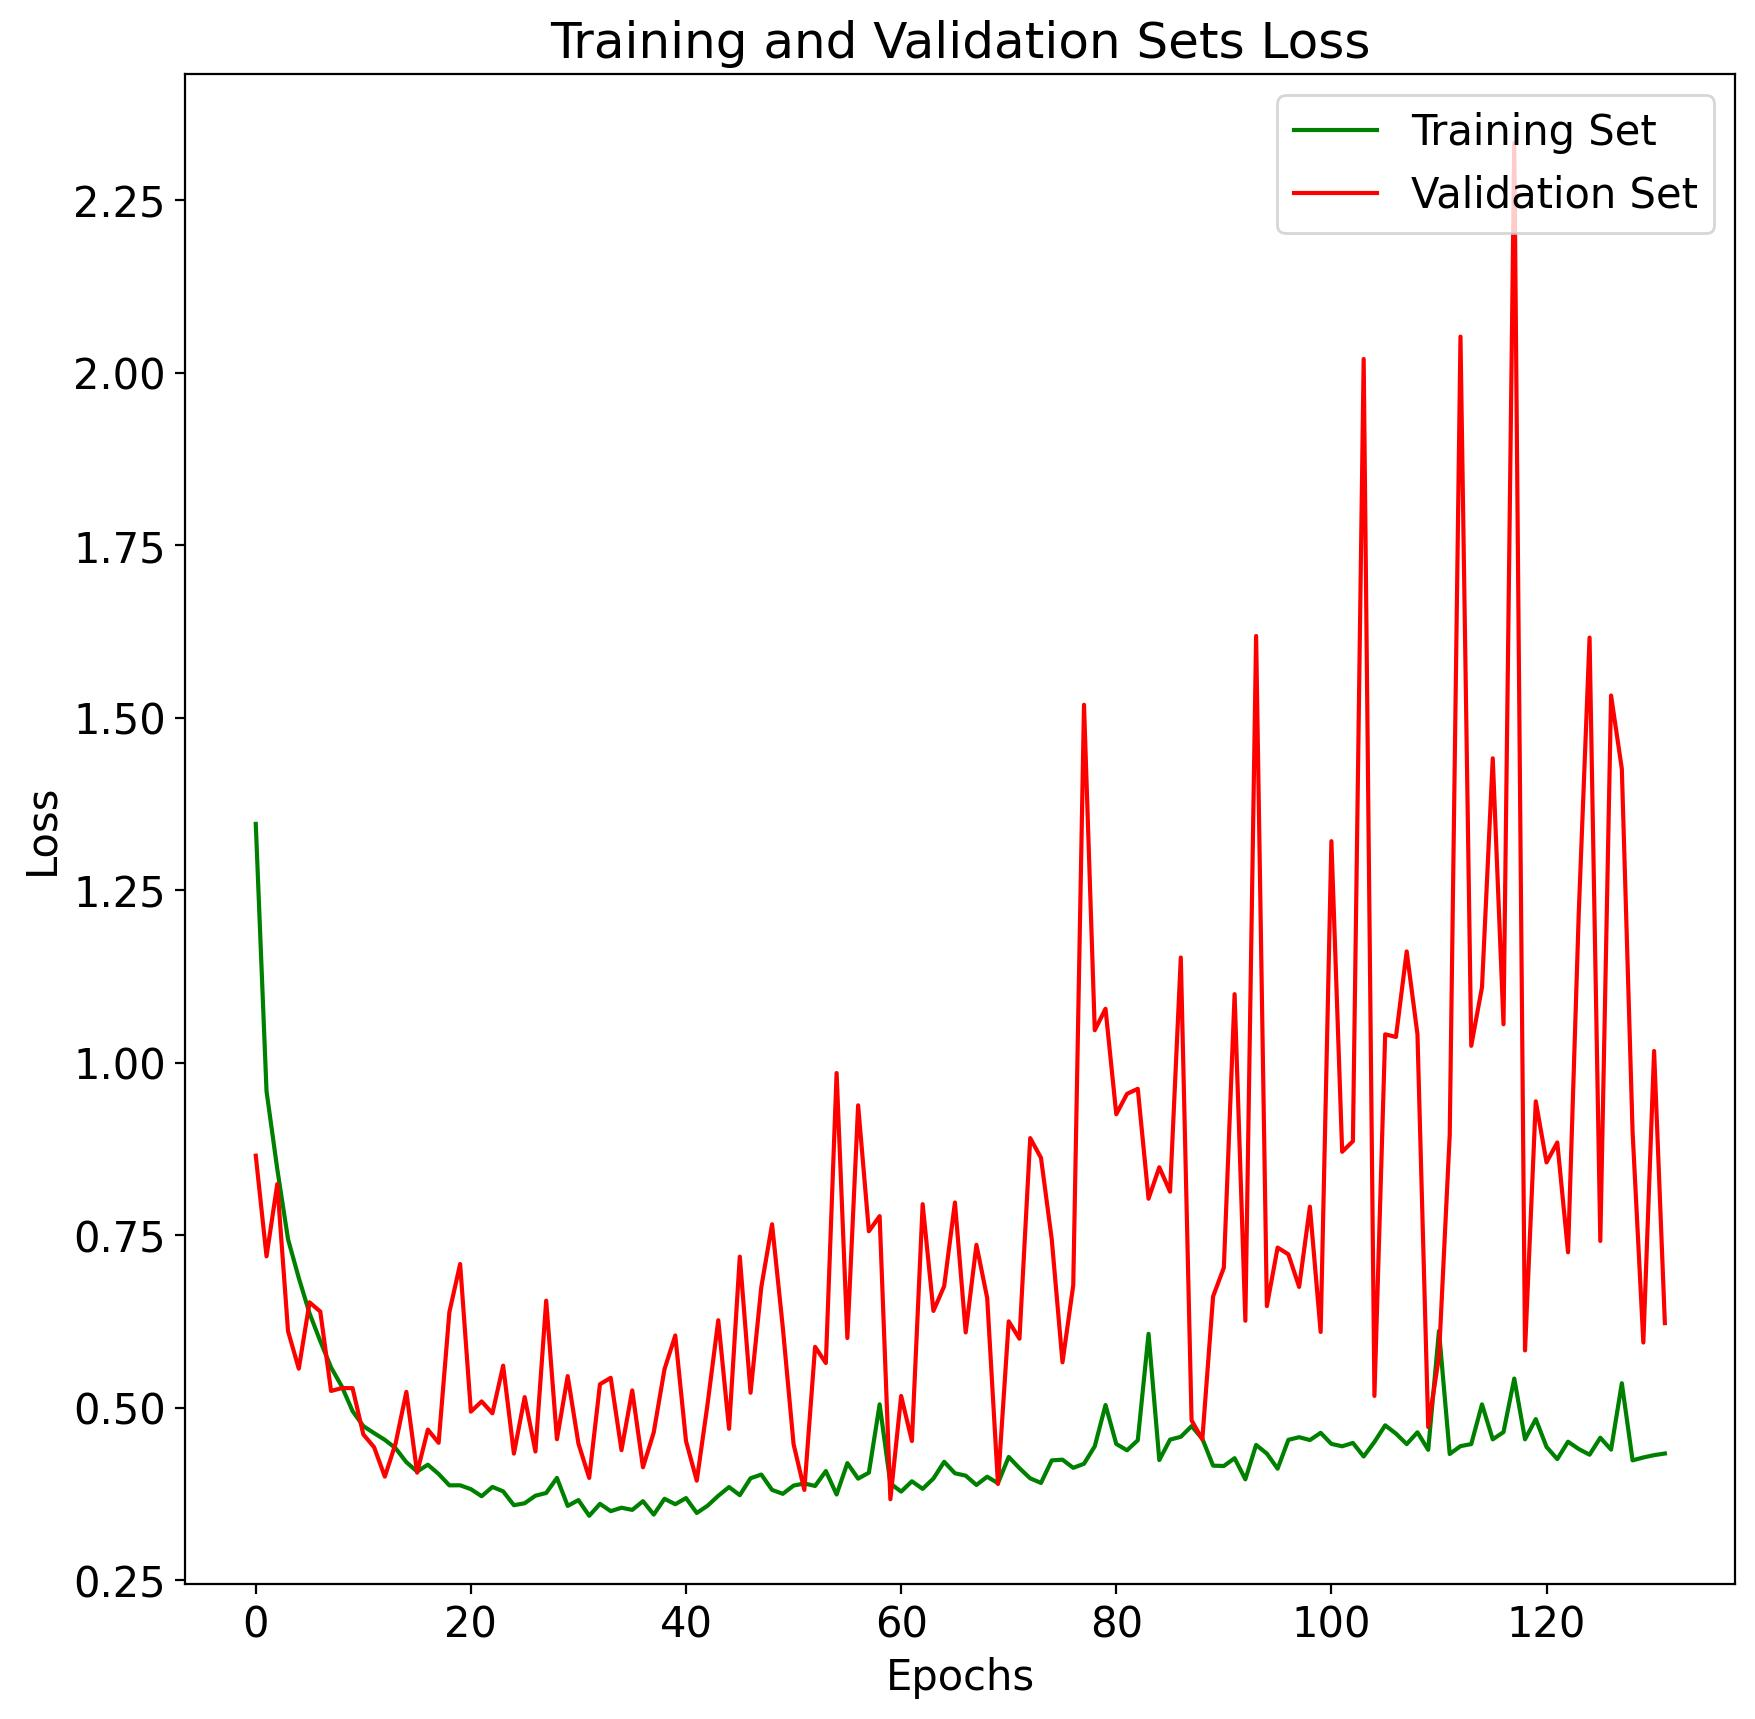
\includegraphics[scale=0.31]{imgs/experiments/images/7/Experiment-7-fold-1.h5-train-val-loss.jpg} }}
    \qquad
    \subfloat[\centering Accuracy]{{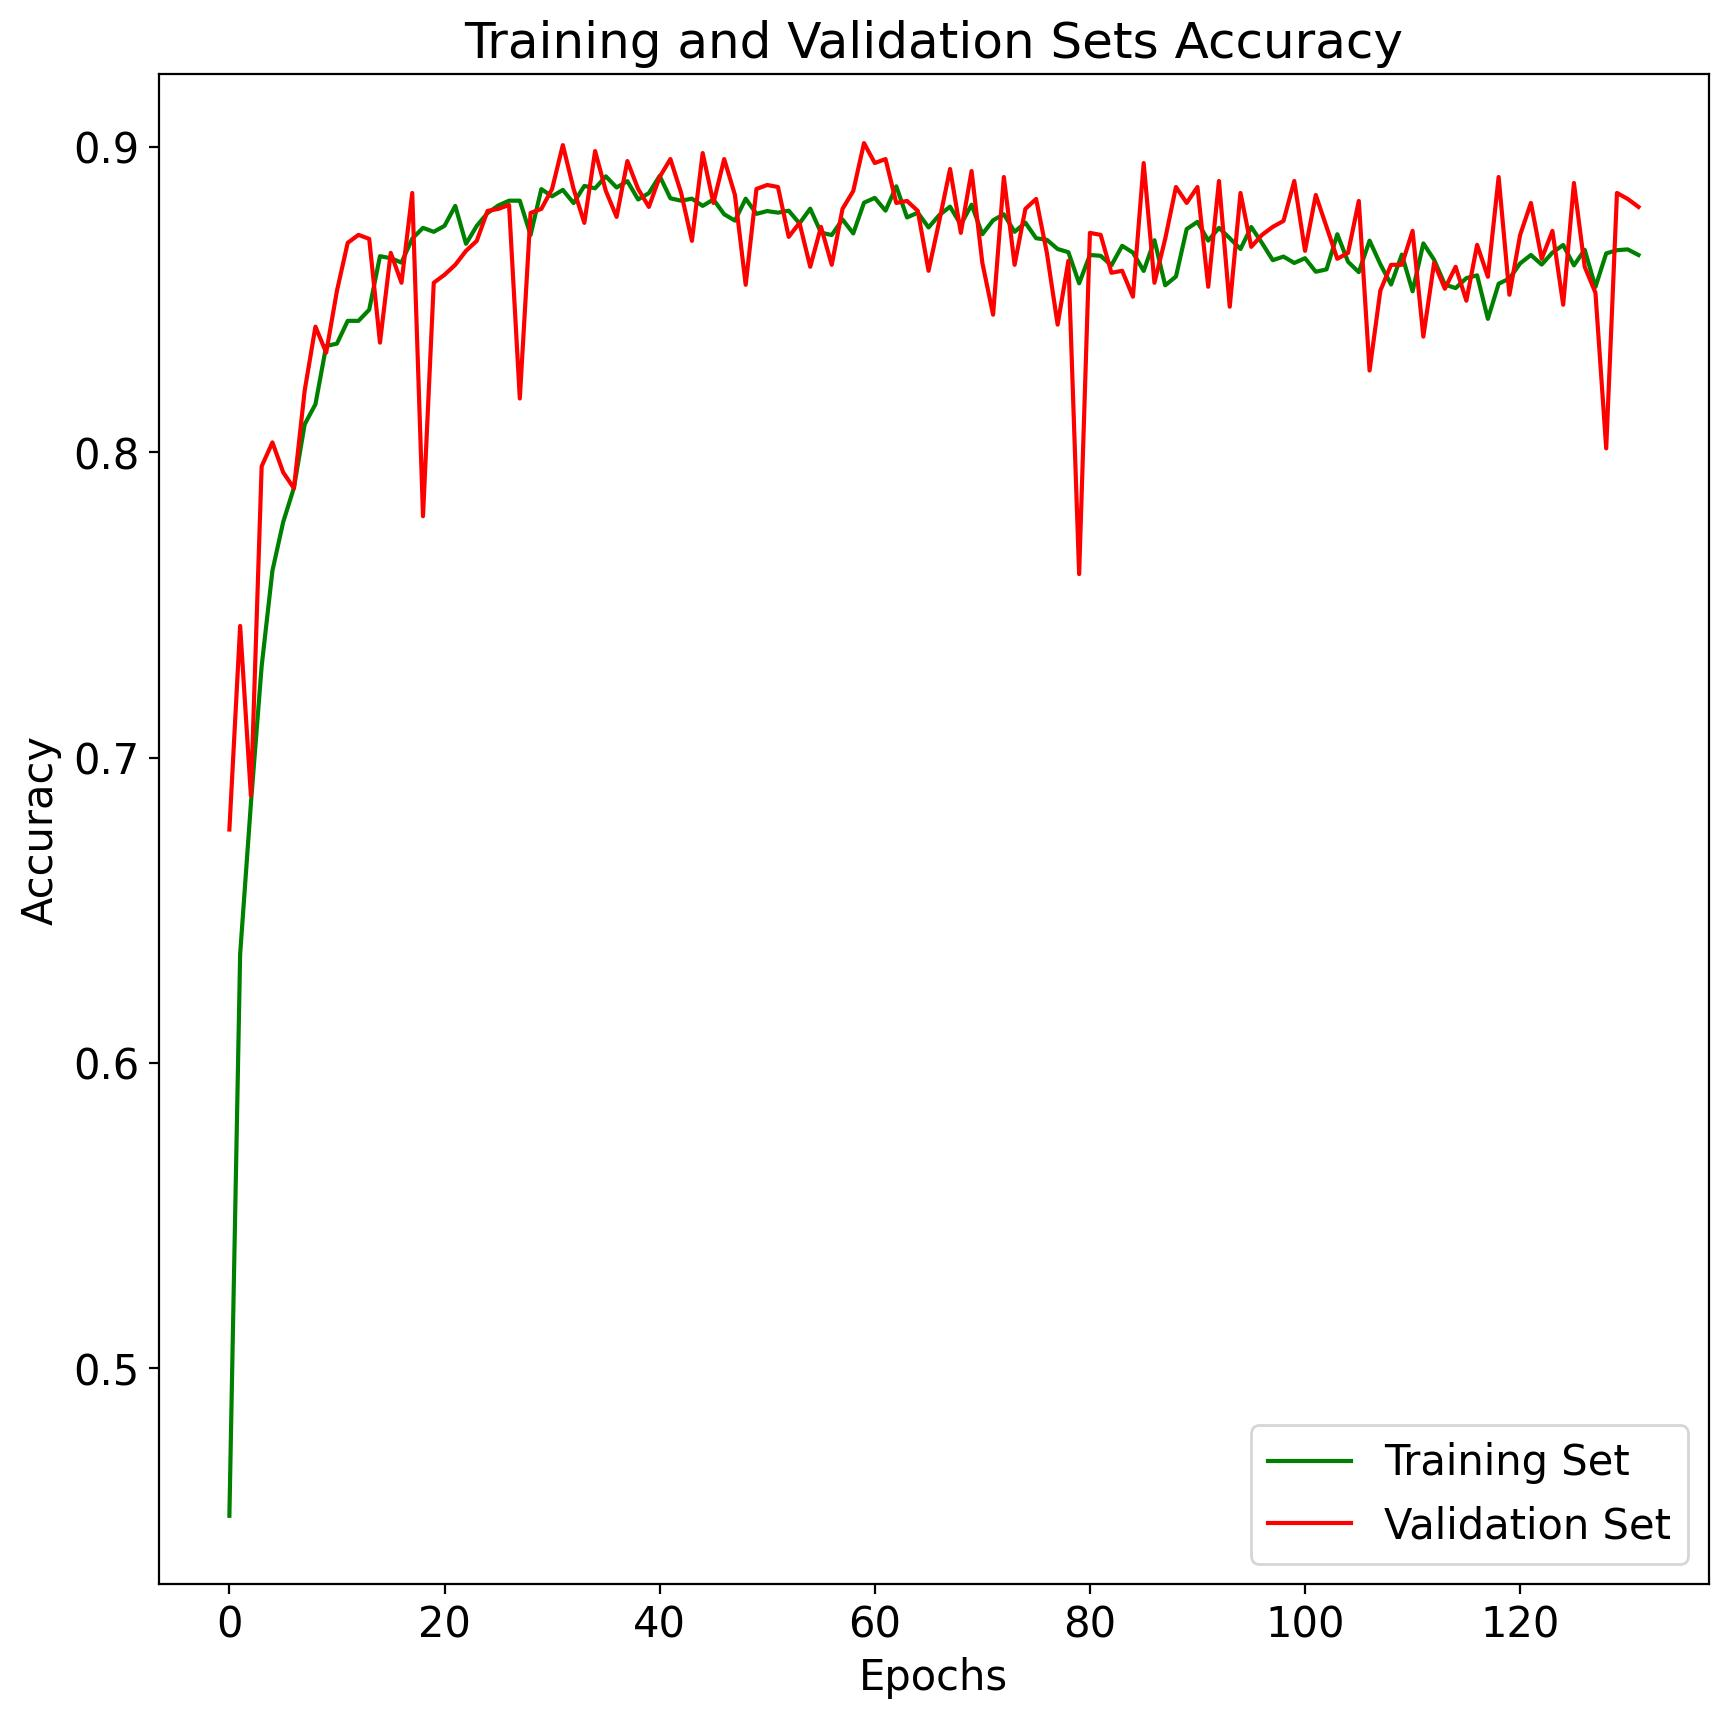
\includegraphics[scale=0.31]{imgs/experiments/images/7/Experiment-7-fold-1.h5-train-val-accuracy.jpg} }}
    \caption{Experiment 7 Results}
\end{figure}
\begin{center}
\hspace*{-0.8cm}
\begin{tabular}{|p{1.2cm}|p{1.8cm}|p{2cm}|p{2cm}|p{2cm}|p{2cm}|p{2cm}|}
\rowcolor{gray!50}
\hline
\textbf{Epoch} & \textbf{Training Loss} & \textbf{Training Accuracy} & \textbf{Validation Loss} & \textbf{Validation Accuracy}\\
\hline
$60$ & $0.3904$ & $0.8818$ & $0.3676$ & $0.9013$\\
\hline
\end{tabular}\\
\end{center}
Using a larger kernel size did not improve the accuracy of the model in a tangible way. By comparing the obtained results with the \texttt{loss} and \texttt{accuracy} plots of the previous experiments it appears that the spikes on the validation set decreased. This trend is visible however only during the initial epochs of training.
\subsection{Experiment 8 (A) - Regularization}
According to Ian Goodfellow, Yoshua Bengio and Aaron Courville in their Deep Learning Book:
\begin{displayquote}
\textit{"In the context of deep learning, most regularization strategies are based on regularizing estimators. Regularization of an estimator works by trading increased bias for reduced variance. An effective regularizer is one that makes a profitable trade, reducing variance significantly while not overly increasing the bias."}
\end{displayquote}
In simple terms, regularization results in simpler models. And as the Occam’s razor principle argues: the simplest models are the most likely to perform better.\\
\\
A first attempt was made using L2 regularization with a value of $0.001$:
\begin{lstlisting}[language=Python,frame=single]
# experiment model layers
layers = [
    Conv2D(32, (5, 5), 'relu', l2(l=0.001), (128, 128, 3)),
    MaxPooling2D((2, 2)),
    Conv2D(64, (4, 4), 'relu', l2(l=0.001)),
    MaxPooling2D((2, 2)),
    Conv2D(128, (3, 3), 'relu', l2(l=0.001)),
    MaxPooling2D((2, 2)),
    Conv2D(256, (3, 3), 'relu', l2(l=0.001)),
    MaxPooling2D((2, 2)),
    Flatten(),
    Dense(128, 'relu', l2(l=0.001)),
    Dropout(0.4),
    Dense(NUM_CLASSES, 'softmax')
]
\end{lstlisting}
Even using \texttt{early stopping}, the training lasted $327$ epochs.
\begin{figure}[H]
    \centering
    \subfloat[\centering Loss]{{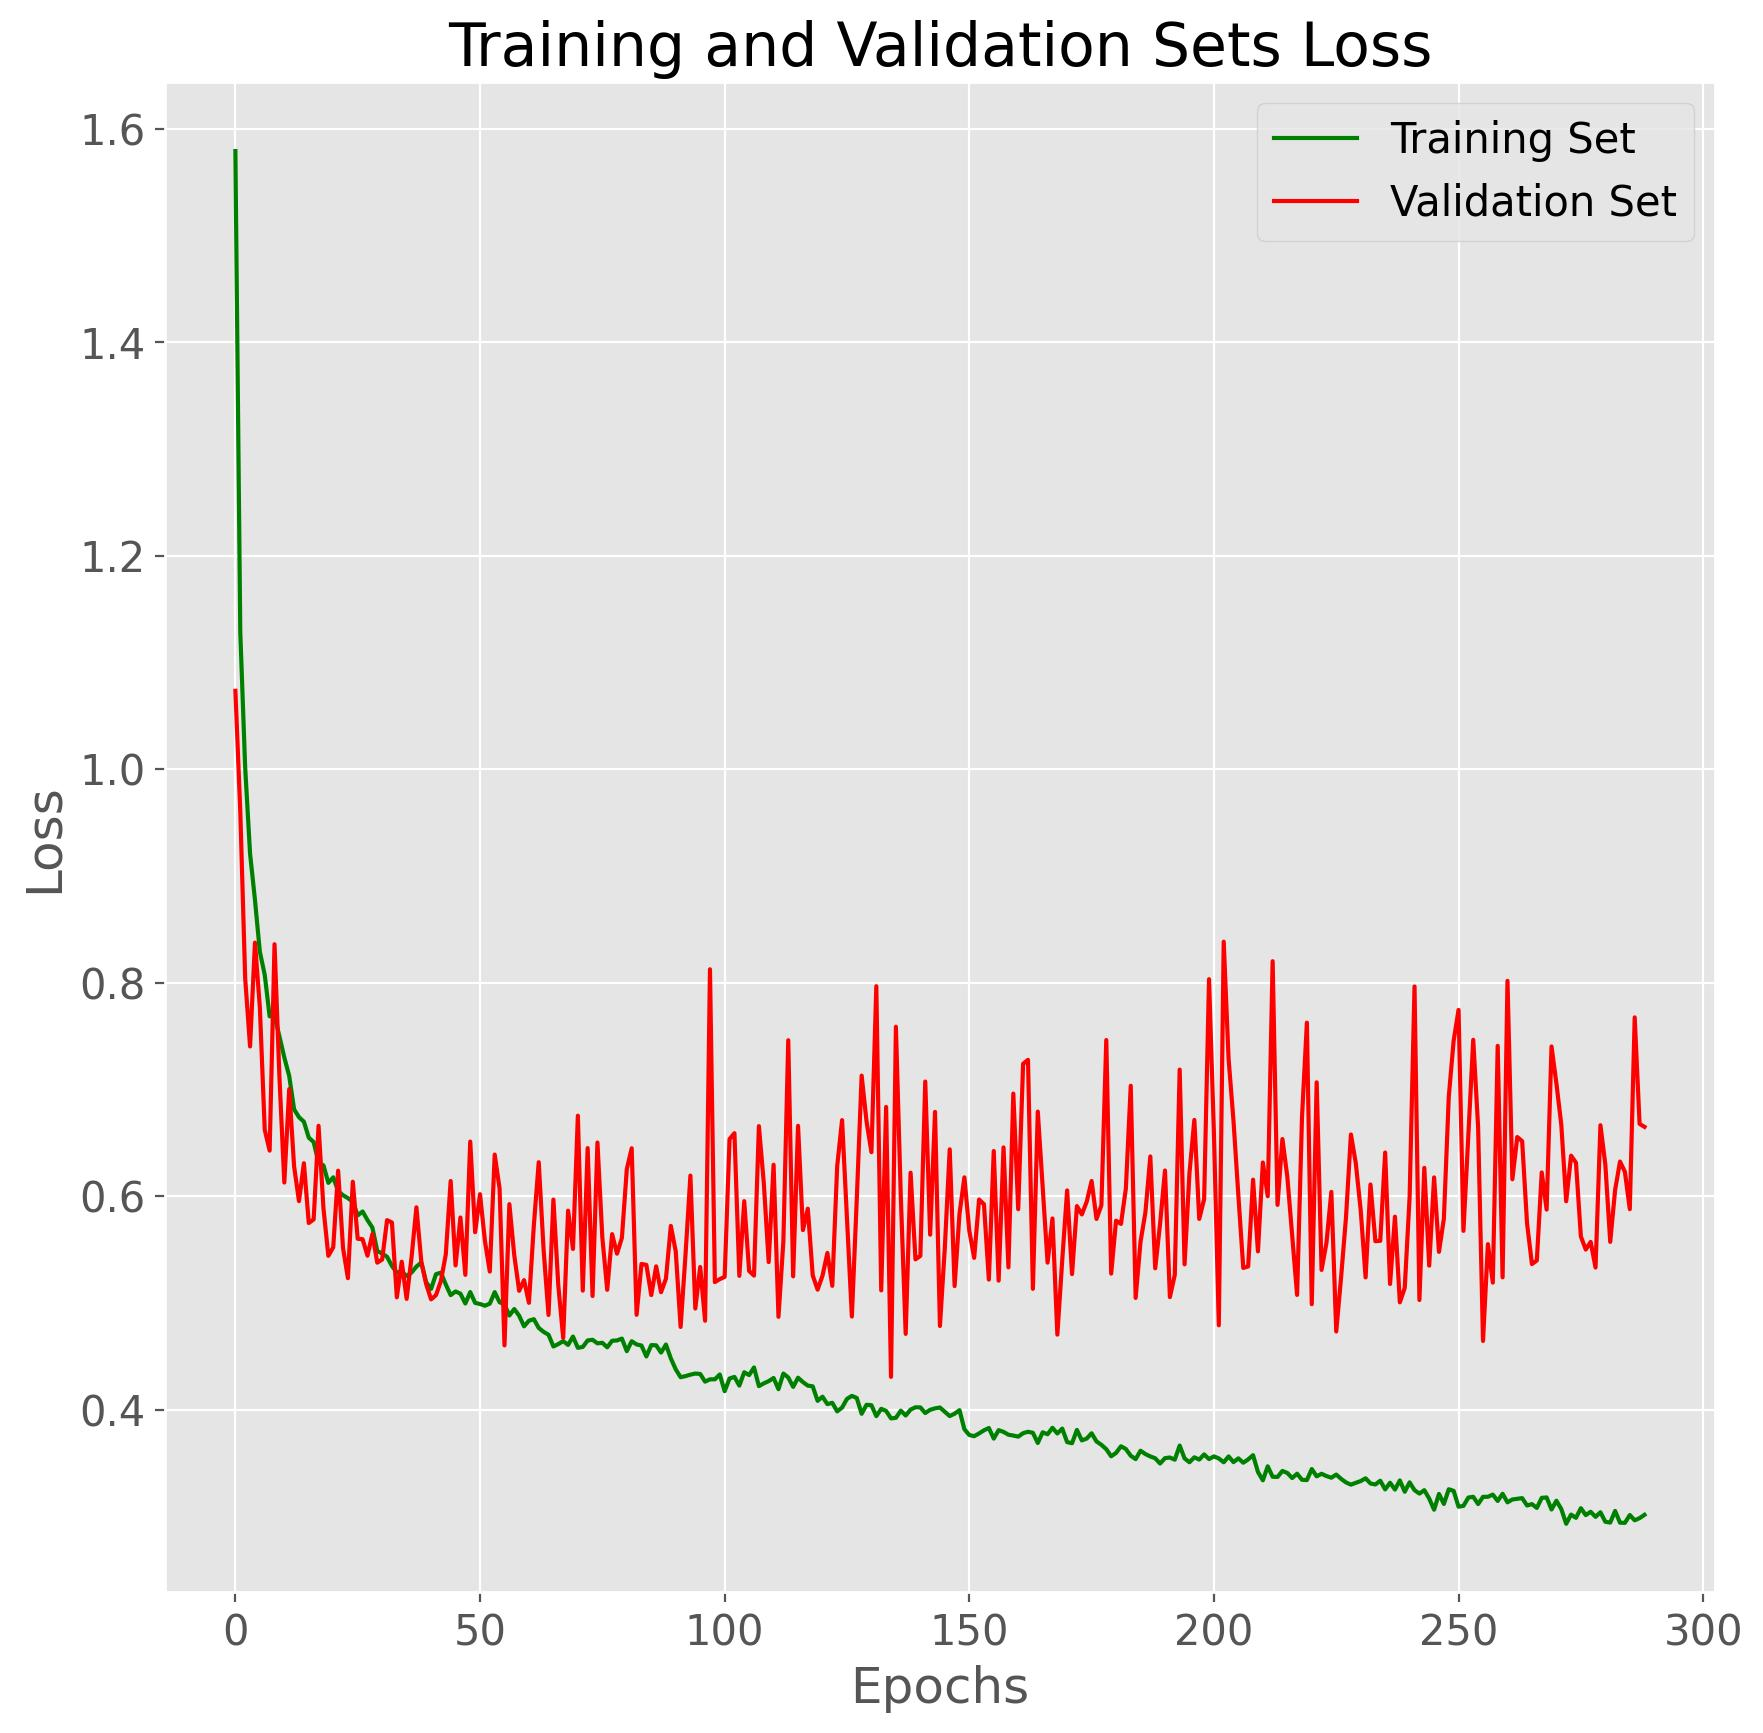
\includegraphics[scale=0.30]{imgs/experiments/images/8-1/Experiment-8-1-fold-1.h5-train-val-loss.jpg} }}
    \qquad
    \subfloat[\centering Accuracy]{{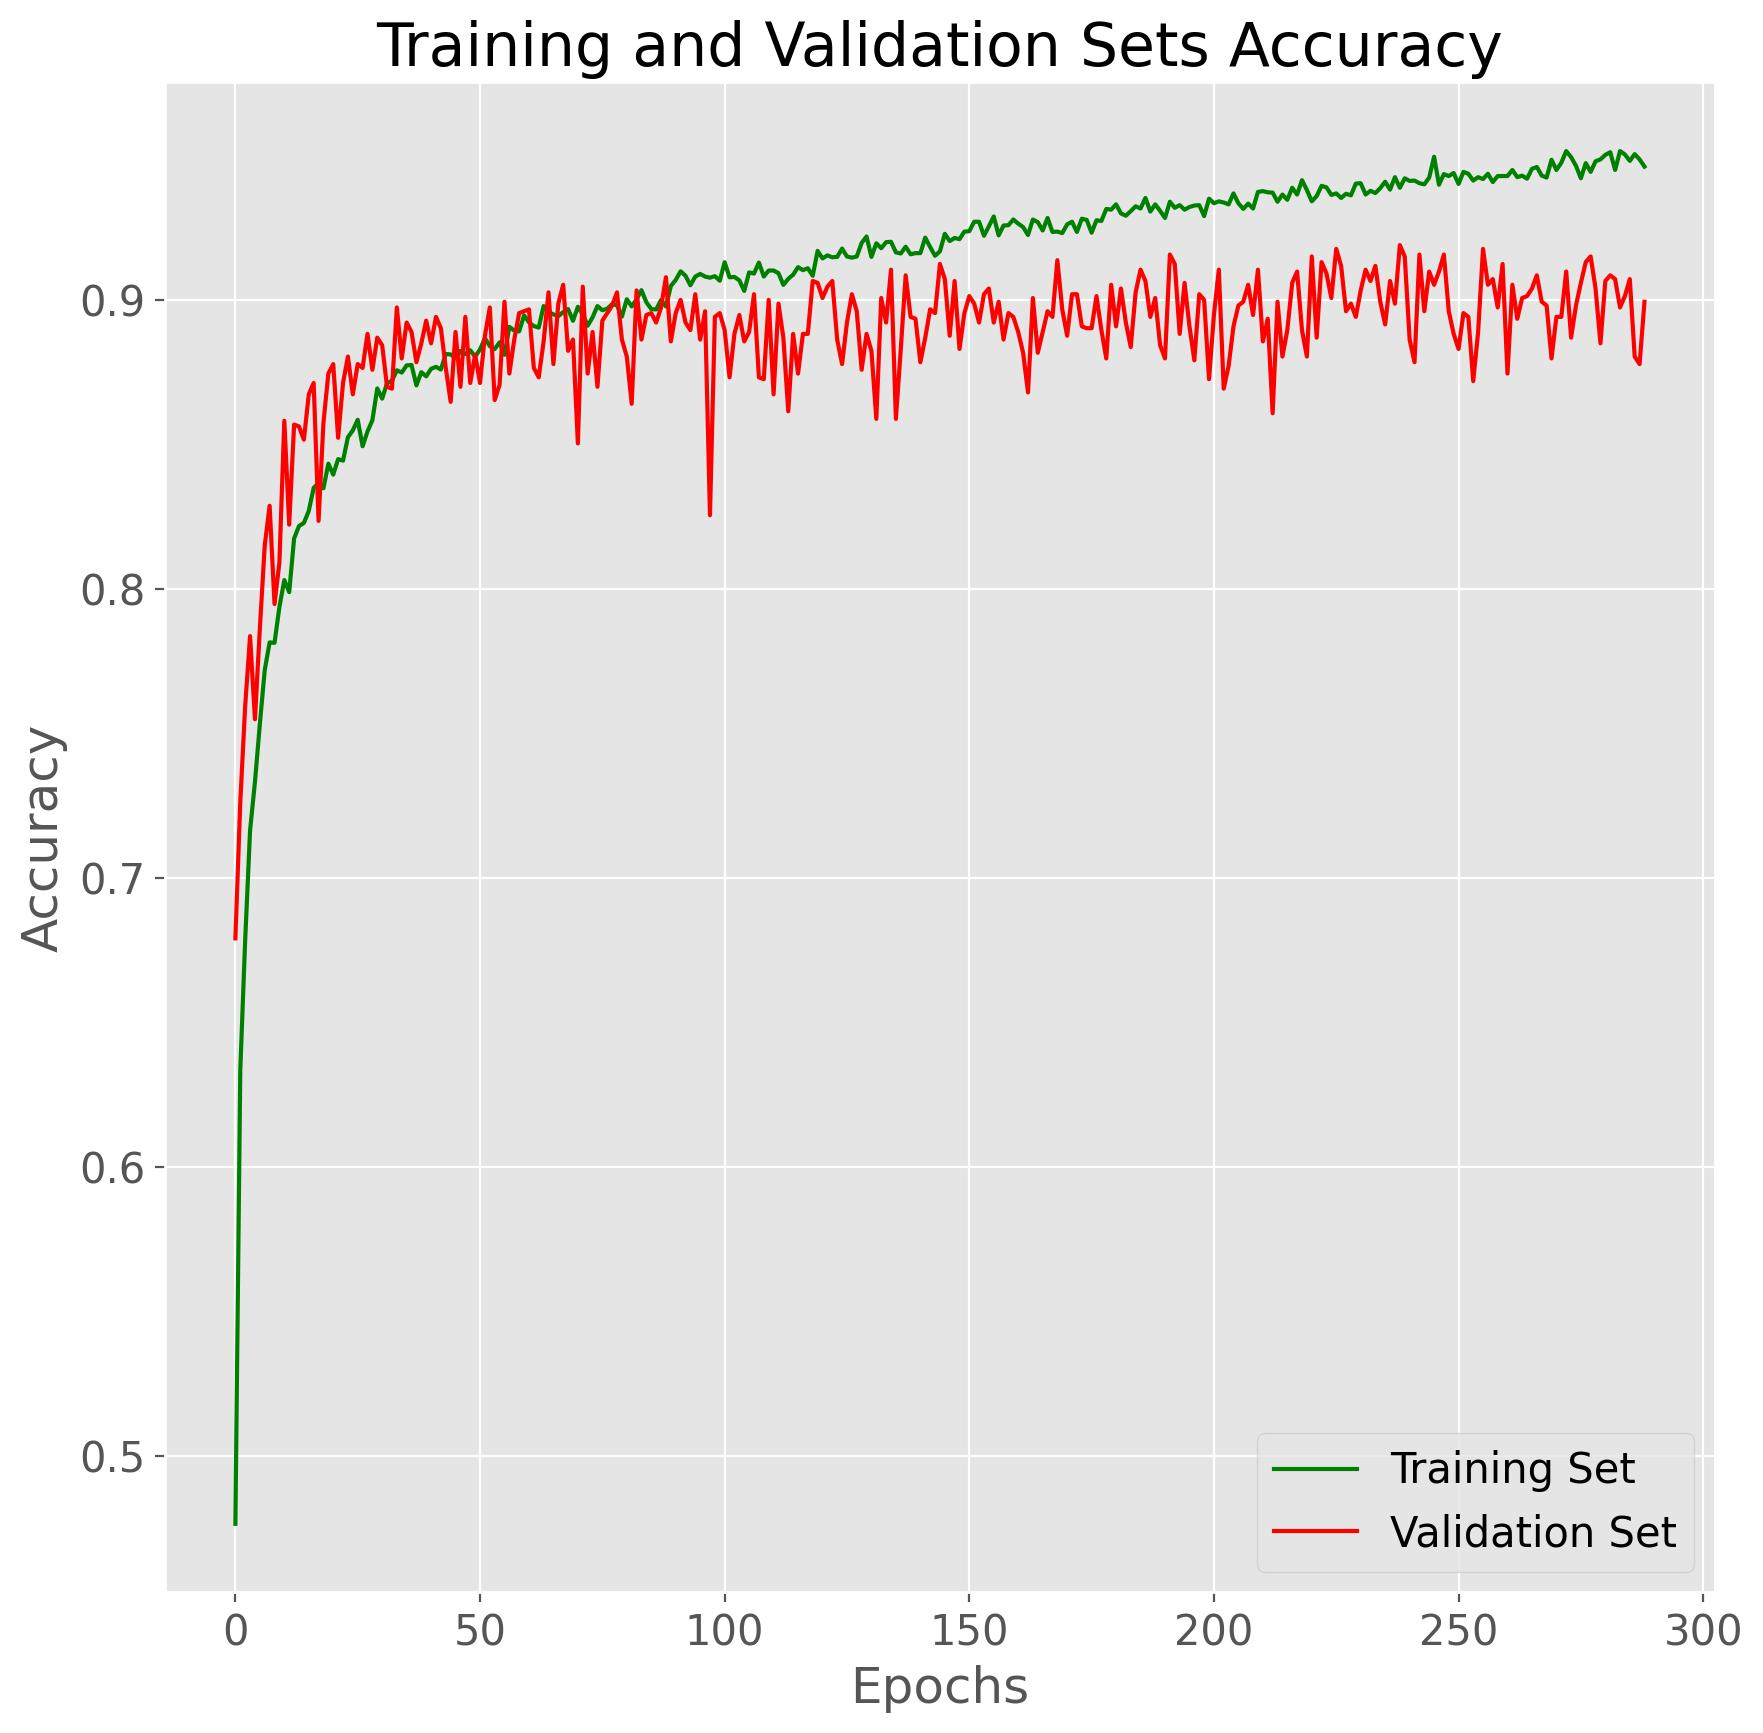
\includegraphics[scale=0.30]{imgs/experiments/images/8-1/Experiment-8-1-fold-1.h5-train-val-accuracy.jpg} }}
    \caption{Experiment 8 (A) Results}
\end{figure}
\noindent
 As a result of using regularization, the \texttt{loss} and \texttt{validation} oscillations actually decreased noticeably. The highest \texttt{loss} spike experienced in previous experiments reached a value of $4.0$ while now the maximum loss overall is lower than $1.0$. One drawback of using this regularization ratio is that the number of training epochs is very high. \texttt{EarlyStopping} is actually never even triggered and the training goes on for the maximum of $300$ epochs.
\begin{center}
\hspace*{-0.8cm}
\begin{tabular}{|p{1.2cm}|p{1.8cm}|p{2cm}|p{2cm}|p{2cm}|p{2cm}|p{2cm}|}
\rowcolor{gray!50}
\hline
\textbf{Epoch} & \textbf{Training Loss} & \textbf{Training Accuracy} & \textbf{Validation Loss} & \textbf{Validation Accuracy}\\
\hline
$135$ & $0.3919$ & $0.9201$ & $0.4308$ & $0.9105$\\
\hline
\end{tabular}\\
\end{center}
\subsection{Experiment 8 (B) - Lower Regularization Factor}
Given that the previous experiment display a very long training time and the benefits were not so high compared to the number of epochs it took for the final model to be trained, I decided to experiment with a reduced value for L2 regularization. In this case, a lower regularization factor of $0.0001$ was used and the following results were obtained after $218$\footnote{More than $100$ epochs less if compared to the previous experiment.}:
\begin{figure}[H]
    \centering
    \subfloat[\centering Loss]{{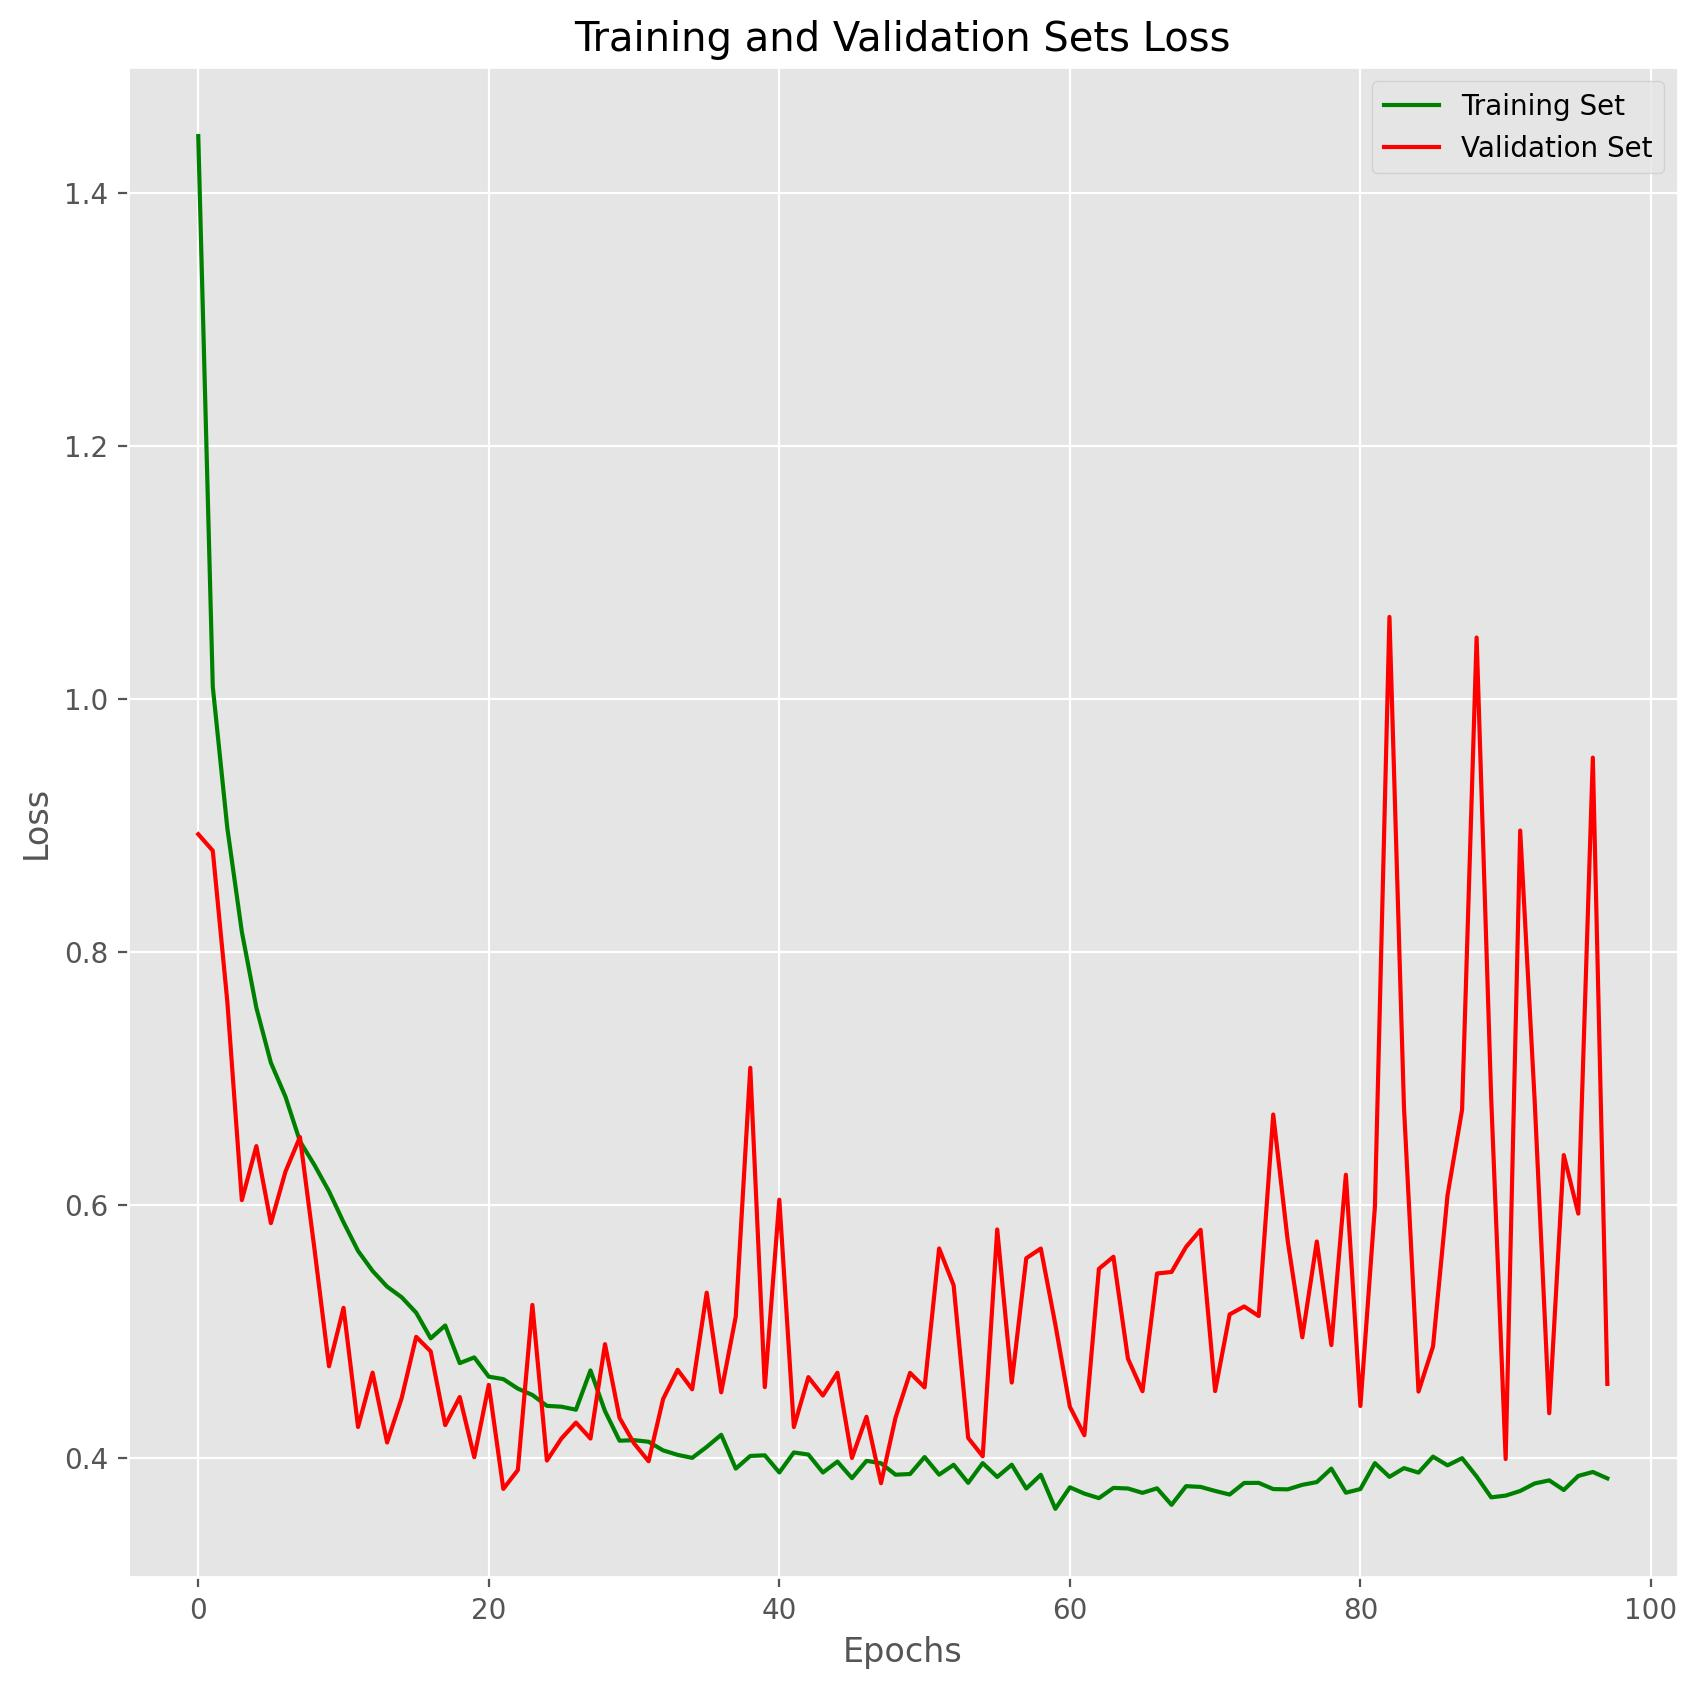
\includegraphics[scale=0.31]{imgs/experiments/images/8-2/Experiment-8-2-fold-1.h5-train-val-loss.jpg} }}
    \qquad
    \subfloat[\centering Accuracy]{{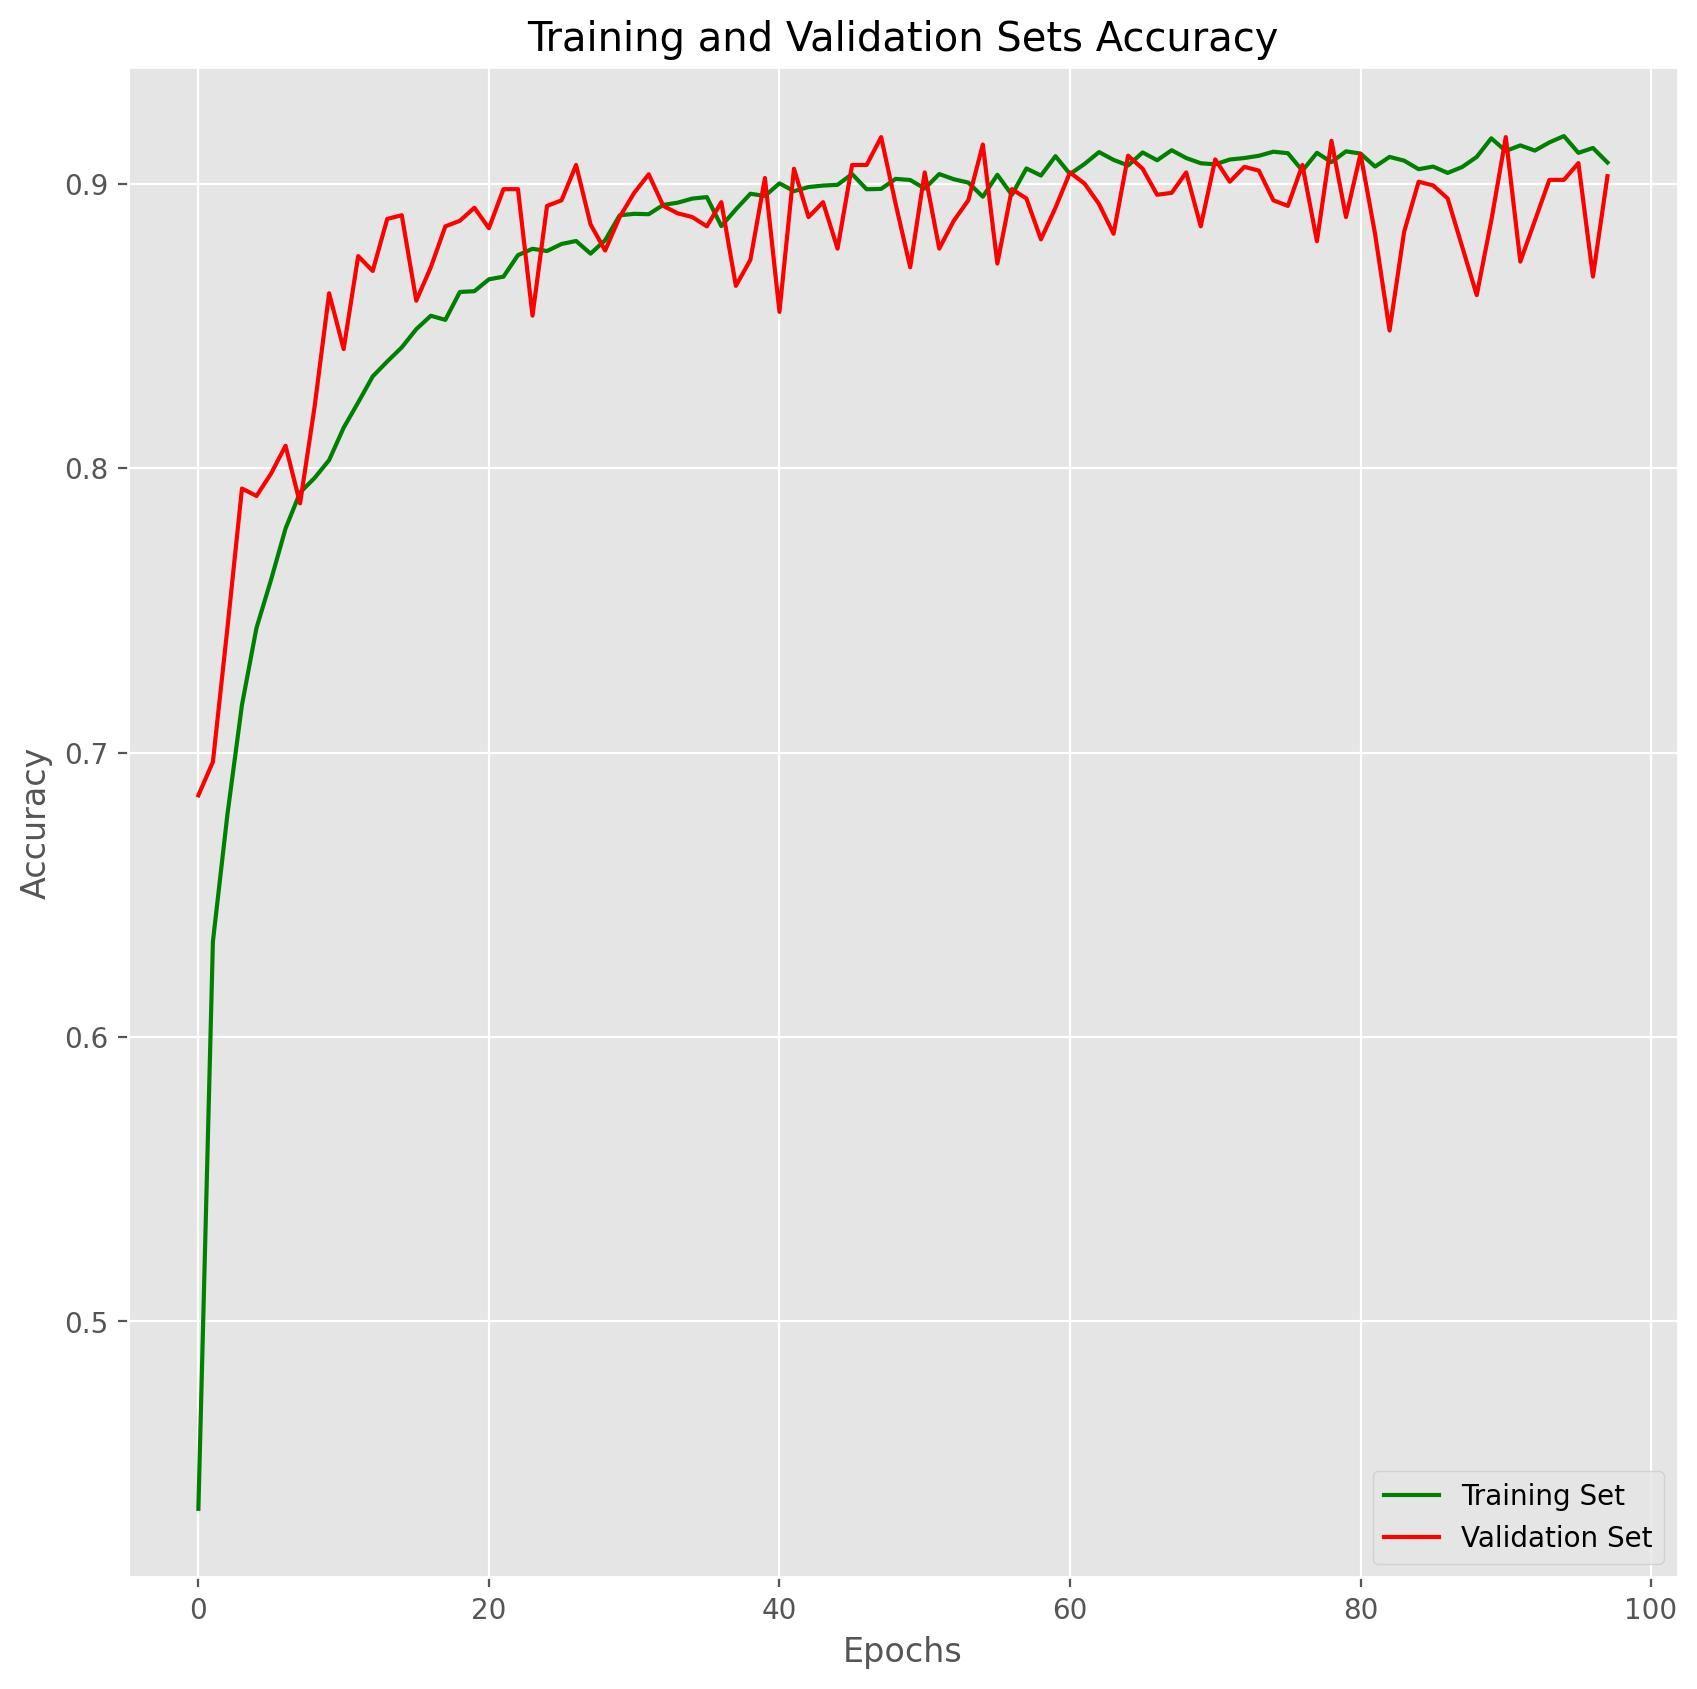
\includegraphics[scale=0.31]{imgs/experiments/images/8-2/Experiment-8-2-fold-1.h5-train-val-accuracy.jpg} }}
    \caption{Experiment 8 (A) Results}
\end{figure}
\begin{center}
\hspace*{-0.8cm}
\begin{tabular}{|p{1.2cm}|p{1.8cm}|p{2cm}|p{2cm}|p{2cm}|p{2cm}|p{2cm}|}
\rowcolor{gray!50}
\hline
\textbf{Epoch} & \textbf{Training Loss} & \textbf{Training Accuracy} & \textbf{Validation Loss} & \textbf{Validation Accuracy}\\
\hline
$22$ & $0.4620$ & $0.8673$ & $0.3752$ & $0.8980$\\
\hline
\end{tabular}\\
\end{center}
Both on the training set and on the validation set, \texttt{loss} scores decreased and \texttt{accuracy} scores increased; additionally, the spikes on the \texttt{loss} values are never higher than $1.0$. The choice was made to use the regularization factor $0.0001$ for the successive experiments.
\subsection{Experiment 9 - Batch Normalization}
Batch Normalization is Indeed one of the major breakthrough in the field of Deep Learning and is one of the hot topics for discussion among researchers in the past few years. Batch Normalization is a widely adopted technique that enables faster and more stable training and has become one of the most influential methods. However, despite its versatility, there are still some points holding this method back.\\
\\
Batch Normalization normalizes the output of the previous output layer by subtracting the empirical mean over the batch divided by the empirical standard deviation. This will help the data look like Gaussian distribution. However, there are many situations under which batch normalization starts to hurt performance or does not work at all. The batch normalization layer has to calculate mean and variance to normalize the previous outputs across the batch. This statistical estimation will be pretty accurate if the batch size is fairly large while keeps on decreasing as the batch size decreases. On the other hand, if the \texttt{batch size} is too high (i.e. $128$) training may not converge. \cite{10.1007/978-3-030-58610-2_14}\\
\\
At this point, the \texttt{batch size} that the model is set to use is $64$; this value was increased gradually throughout the different experiments in order to achieve a smoother learning process. Because of this uncertainty, \textbf{3 similar experiments where performed with different batch sizes}: the \textit{BatchNormalization} layer is added right after the \texttt{Conv2D}. Each of the experiments was performed with a different \texttt{batch size}: $128$, $64$ and $32$ respectively.\\
Additionally \texttt{early stopping} parameters were changed from \texttt{min\_delta=0.01, patience=100} to \texttt{min\_delta=0.001, patience=50} in order to decrease the high number of training epochs.\\
\\
The results obtained are plotted in the following pictures:
\begin{figure}[H]
    \centering
    \subfloat[\centering Loss]{{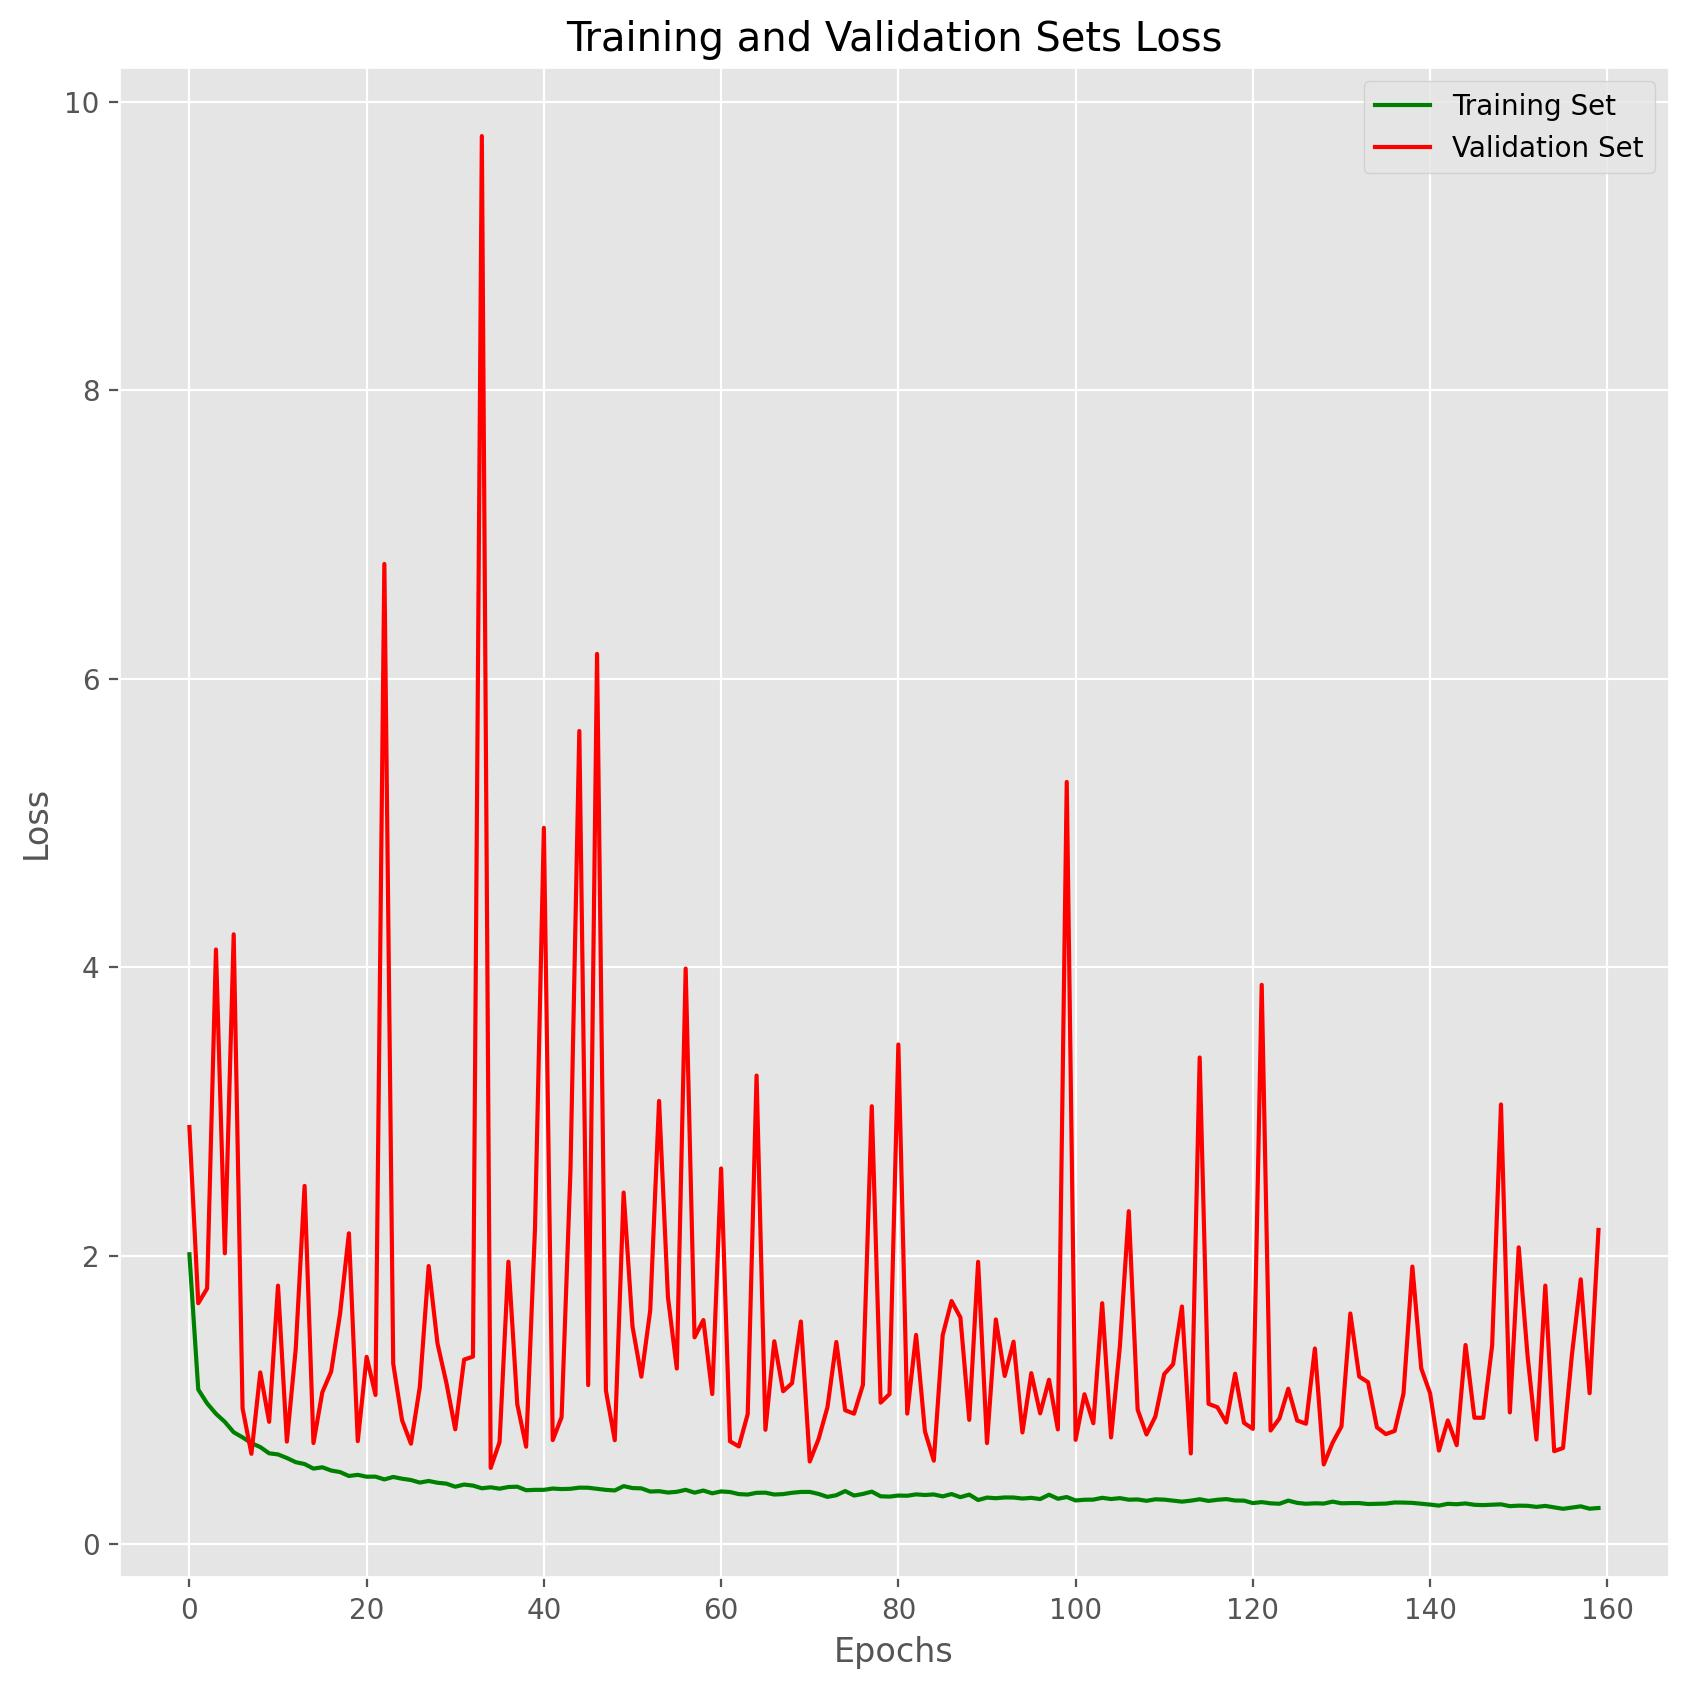
\includegraphics[scale=0.31]{imgs/experiments/images/9-1/Experiment-9-1-fold-1.h5-train-val-loss.jpg} }}
    \qquad
    \subfloat[\centering Accuracy]{{\includegraphics[scale=0.31]{imgs/experiments/images/9-1/Experiment-9-1-fold-1.h5-train-val-accuracy.jpg} }}
    \caption{Experiment 9 Results - Batch Size: 128}
\end{figure}
\begin{center}
\hspace*{-0.8cm}
\begin{tabular}{|p{1.2cm}|p{1.8cm}|p{2cm}|p{2cm}|p{2cm}|p{2cm}|p{2cm}|}
\rowcolor{gray!50}
\hline
\textbf{Epoch} & \textbf{Training Loss} & \textbf{Training Accuracy} & \textbf{Validation Loss} & \textbf{Validation Accuracy}\\
\hline
$35$ & $0.3937$ & $0.9036$ & $0.5284$ & $0.8935$\\
\hline
\end{tabular}\\
\end{center}
\begin{figure}[H]
    \centering
    \subfloat[\centering Loss]{{\includegraphics[scale=0.31]{imgs/experiments/images/9-2/Experiment-9-2-fold-1.h5-train-val-loss.jpg} }}
    \qquad
    \subfloat[\centering Accuracy]{{\includegraphics[scale=0.31]{imgs/experiments/images/9-2/Experiment-9-2-fold-1.h5-train-val-accuracy.jpg} }}
    \caption{Experiment 9 Results - Batch Size: 64}
\end{figure}
\begin{center}
\hspace*{-0.8cm}
\begin{tabular}{|p{1.2cm}|p{1.8cm}|p{2cm}|p{2cm}|p{2cm}|p{2cm}|p{2cm}|}
\rowcolor{gray!50}
\hline
\textbf{Epoch} & \textbf{Training Loss} & \textbf{Training Accuracy} & \textbf{Validation Loss} & \textbf{Validation Accuracy}\\
\hline
$102$ & $0.3565$ & $0.9434$ & $0.5704$ & $0.9000$\\
\hline
\end{tabular}\\
\end{center}
\begin{figure}[H]
    \centering
    \subfloat[\centering Loss]{{\includegraphics[scale=0.31]{imgs/experiments/images/9-3/Experiment-9-3-fold-1.h5-train-val-loss.jpg} }}
    \qquad
    \subfloat[\centering Accuracy]{{\includegraphics[scale=0.31]{imgs/experiments/images/9-3/Experiment-9-3-fold-1.h5-train-val-accuracy.jpg} }}
    \caption{Experiment 9 Results - Batch Size: 32}
\end{figure}
\begin{center}
\hspace*{-0.8cm}
\begin{tabular}{|p{1.2cm}|p{1.8cm}|p{2cm}|p{2cm}|p{2cm}|p{2cm}|p{2cm}|}
\rowcolor{gray!50}
\hline
\textbf{Epoch} & \textbf{Training Loss} & \textbf{Training Accuracy} & \textbf{Validation Loss} & \textbf{Validation Accuracy}\\
\hline
$149$ & $0.3541$ & $0.9370$ & $0.5275$ & $0.9196$\\
\hline
\end{tabular}\\
\end{center}
Taking into account the results achieved in the different experiments, the following considerations can be made:
\begin{itemize}
    \item no tangible improvement in the accuracy on the validation set was achieved;
    \item spikes on both the \texttt{loss} and \texttt{accuracy} reached unprecedented maximums.
\end{itemize}

\newpage
\section{Task 3: Pre-trained - Images}
The implementation of what is described in this section can be found in the Jupyter Notebook named \texttt{Task3-Pre-trained-images.ipynb}.\\
\\
The \texttt{tf.keras.applications} package provides deep learning models that are made available alongside pre-trained weights. A pre-trained model is a saved network that was previously trained on a large dataset, typically on a large-scale image-classification task. You either use the pre-trained model as is or use transfer learning to customize this model to a given task. The intuition behind transfer learning for image classification is that if a model is trained on a large and general enough dataset, this model will effectively serve as a generic model of the visual world. You can then take advantage of these learned feature maps without having to start from scratch by training a large model on a large dataset.\\
\\
In the following sections some pre-trained models were customized in two ways:
\begin{itemize}
    \item \textbf{Feature Extraction:} Use the representations learned by a previous network to extract meaningful features from new samples.
    \item \textbf{Fine-Tuning:} Unfreeze a few of the top layers of a frozen model base and jointly train both the newly-added classifier layers and the last layers of the base model.
\end{itemize}
\subsection{Classes Correspondence}
Before jumping into training and tuning pre-trained models, I checked that this was actually suitable given the classes of our interest.
After consulting the list of the classes found in the \texttt{Imagenet}\footnote{ImageNet Classes list: \url{https://deeplearning.cms.waikato.ac.nz/user-guide/class-maps/IMAGENET/}} dataset, the following correspondences between our selected classes and the ones of \texttt{Imagenet} were found:
\begin{itemize}
    \item Table $\longrightarrow$ dining table, board;
    \item Chair $\longrightarrow$ barber chair, folding chair, rocking chair, rocker;
    \item Lamp $\longrightarrow$ lampshade, lamp shade, table lamp;
    \item Dresser $\longrightarrow$ wardrobe, closet, press;
    \item Sofa $\longrightarrow$ studio couch, day bed;
\end{itemize}
Enough similarities are found in common between the original dataset and the \texttt{Imagenet} dataset.
\subsection{VGG16}
VGG16 is a convolution neural net (CNN) architecture which was used to win ILSVR (Imagenet) competition in 2014. It is considered to be one of the excellent vision model architecture till date. Most unique thing about VGG16 is that instead of having a large number of hyper-parameter they focused on having convolution layers of $3$x$3$ filter with a stride $1$ and always used same padding and Maxpool layer of $2$x$2$ filter of stride $2$. It follows this arrangement of convolution and max pool layers consistently throughout the whole architecture. In the end it has $2$ FC (fully connected layers) followed by a softmax for output. The $16$ in VGG16 refers to it has $16$ layers that have weights. This network is a pretty large network and it has about $138$ million (approx) parameters.
\begin{figure}[H]
    \centering
    \includegraphics[scale=0.45]{imgs/vgg16.png}
    \caption{VGG16 Architecture}
\end{figure}
\subsubsection{Feature Extraction}
\paragraph{Experiment 0 - When things go wrong}\mbox{}\\
In the first experiment that was attempted, a big mistake was committed. The input data was preprocessed before feeding such data to the preprocessing pipeline of \texttt{VGG16}. This resulted in very poor performances, the network did not learn much. The choice was made to include the results obtained as \textbf{learnt lesson}.
\begin{lstlisting}[language=Python,frame=single]
# define convolutional base
vgg16_conv_base = vgg16.VGG16(
    weights="imagenet",
    include_top=False,
    input_shape=(128, 128, 3))

# freeze convolutional base
vgg16_conv_base.trainable = False

# define model with classifier
inputs = Input(shape=(128, 128, 3))
x = vgg16.preprocess_input(inputs)
x = vgg16_conv_base(x)
x = Flatten()(x)
x = Dense(256, activation='relu')(x)
outputs = Dense(NUM_CLASSES, activation="softmax")(x)
model = Model(inputs, outputs)
\end{lstlisting}
The training took $264$ producing the results displayed below:
\begin{figure}[H]
    \centering
    \subfloat[\centering Loss]{{\includegraphics[scale=0.3]{imgs/experiments/images/10/Experiment-10-fold-1.h5-train-val-loss.jpg} }}
    \qquad
    \subfloat[\centering Accuracy]{{\includegraphics[scale=0.3]{imgs/experiments/images/10/Experiment-10-fold-1.h5-train-val-accuracy.jpg} }}
    \caption{Experiment 0 Results}
\end{figure}
\begin{center}
\hspace*{-0.8cm}
\begin{tabular}{|p{1.2cm}|p{1.8cm}|p{2cm}|p{2cm}|p{2cm}|p{2cm}|p{2cm}|}
\rowcolor{gray!50}
\hline
\textbf{Epoch} & \textbf{Training Loss} & \textbf{Training Accuracy} & \textbf{Validation Loss} & \textbf{Validation Accuracy}\\
\hline
$254$ & $1.1172$ & $0.5719$ & $1.1272$ & $0.5796$\\
\hline
\end{tabular}\\
\end{center}
\paragraph{Experiment 1 - No custom preprocessing}\mbox{}\\
In this second attempt, everything was done correctly and the following results were obtained after $100$ epochs of training:
\begin{lstlisting}[language=Python,frame=single]
# define convolutional base
vgg16_conv_base = vgg16.VGG16(
    weights="imagenet",
    include_top=False,
    input_shape=(128, 128, 3))

# freeze convolutional base
vgg16_conv_base.trainable = False

# define model with classifier
inputs = Input(shape=(128, 128, 3))
x = vgg16.preprocess_input(inputs)
x = vgg16_conv_base(x)
x = Flatten()(x)
x = Dense(256, activation='relu')(x)
outputs = Dense(NUM_CLASSES, activation="softmax")(x)
model = Model(inputs, outputs)
\end{lstlisting}
The training took $198$ producing the results displayed below:
\begin{figure}[H]
    \centering
    \subfloat[\centering Loss]{{\includegraphics[scale=0.3]{imgs/experiments/images/11/Experiment-11-fold-1.h5-train-val-loss.jpg} }}
    \qquad
    \subfloat[\centering Accuracy]{{\includegraphics[scale=0.3]{imgs/experiments/images/11/Experiment-11-fold-1.h5-train-val-accuracy.jpg} }}
    \caption{Experiment 1 Results}
\end{figure}
\begin{center}
\hspace*{-0.8cm}
\begin{tabular}{|p{1.2cm}|p{1.8cm}|p{2cm}|p{2cm}|p{2cm}|p{2cm}|p{2cm}|}
\rowcolor{gray!50}
\hline
\textbf{Epoch} & \textbf{Training Loss} & \textbf{Training Accuracy} & \textbf{Validation Loss} & \textbf{Validation Accuracy}\\
\hline
$3$ & $0.5634$ & $0.8716$ & $0.5968$ & $0.8935$\\
\hline
\end{tabular}\\
\end{center}
Overfitting is immediately visible right after $3$ epochs of training. After less than $100$ epochs of training the network achieved an accuracy of $99\%$ on the training set.
\paragraph{Experiment 2 - Dropout}\mbox{}\\
Starting from the results obtained in the previous experiment, the focus is now on reducing overfitting as much as possible.\\
\\
Additionally, \texttt{early stopping} parameters were changed from \texttt{min\_delta=0.01, patience=100} to \texttt{min\_delta=0.001, patience=50} in order to decrease the high number of training epochs.
\begin{lstlisting}[language=bash,frame=single]
# define convolutional base
vgg16_conv_base = vgg16.VGG16(
    weights="imagenet",
    include_top=False,
    input_shape=(128, 128, 3))

# freeze convolutional base
vgg16_conv_base.trainable = False

# define model with classifier
inputs = Input(shape=(128, 128, 3))
x = vgg16.preprocess_input(inputs)
x = vgg16_conv_base(x)
x = Flatten()(x)
x = Dense(256, activation='relu')(x)
x = Dropout(0.4)(x)
outputs = Dense(NUM_CLASSES, activation="softmax")(x)
model = Model(inputs, outputs)
\end{lstlisting}
The training took $100$ epochs producing the results displayed below:
\begin{figure}[H]
    \centering
    \subfloat[\centering Loss]{{\includegraphics[scale=0.3]{imgs/experiments/images/12/Experiment-12-fold-1.h5-train-val-loss.jpg} }}
    \qquad
    \subfloat[\centering Accuracy]{{\includegraphics[scale=0.3]{imgs/experiments/images/12/Experiment-12-fold-1.h5-train-val-accuracy.jpg} }}
    \caption{Experiment 2 Results}
\end{figure}
\begin{center}
\hspace*{-0.8cm}
\begin{tabular}{|p{1.2cm}|p{1.8cm}|p{2cm}|p{2cm}|p{2cm}|p{2cm}|p{2cm}|}
\rowcolor{gray!50}
\hline
\textbf{Epoch} & \textbf{Training Loss} & \textbf{Training Accuracy} & \textbf{Validation Loss} & \textbf{Validation Accuracy}\\
\hline
$8$ & $0.5250$ & $0.8824$ & $0.5819$ & $0.9092$\\
\hline
\end{tabular}\\
\end{center}
\paragraph{Experiment 3 - Smaller FC, Increased Dropout, Longer Training}\mbox{}\\
In the previous experiment, overfitting starts to appear right after epoch $30$. It is probably more visible on the \texttt{loss} plot rather than the \texttt{accuracy} plot. A third experiment was attempted by reducing the fully connected layer size from $256$ to $128$, increasing the \texttt{dropout} drop ratio from $0.4$ to $0.5$. The maximum number of training epochs was also increased to $200$:
\begin{lstlisting}[language=bash,frame=single]
# define convolutional base
vgg16_conv_base = vgg16.VGG16(
    weights="imagenet",
    include_top=False,
    input_shape=(128, 128, 3))

# freeze convolutional base
vgg16_conv_base.trainable = False

# define model with classifier
inputs = Input(shape=(128, 128, 3))
x = vgg16.preprocess_input(inputs)
x = vgg16_conv_base(x)
x = Flatten()(x)
x = Dense(128, activation='relu')(x)
x = Dropout(0.5)(x)
outputs = Dense(NUM_CLASSES, activation="softmax")(x)
model = Model(inputs, outputs)
\end{lstlisting}
The training took $133$ epochs producing the results displayed below:
\begin{figure}[H]
    \centering
    \subfloat[\centering Loss]{{\includegraphics[scale=0.3]{imgs/experiments/images/13/Experiment-13-fold-1.h5-train-val-loss.jpg} }}
    \qquad
    \subfloat[\centering Accuracy]{{\includegraphics[scale=0.3]{imgs/experiments/images/13/Experiment-13-fold-1.h5-train-val-accuracy.jpg} }}
    \caption{Experiment 3 Results}
\end{figure}
\begin{center}
\hspace*{-0.8cm}
\begin{tabular}{|p{1.2cm}|p{1.8cm}|p{2cm}|p{2cm}|p{2cm}|p{2cm}|p{2cm}|}
\rowcolor{gray!50}
\hline
\textbf{Epoch} & \textbf{Training Loss} & \textbf{Training Accuracy} & \textbf{Validation Loss} & \textbf{Validation Accuracy}\\
\hline
$13$ & $0.6240$ & $0.8603$ & $0.5777$ & $0.9072$\\
\hline
\end{tabular}\\
\end{center}
Even if the problem was not solved completely, it improved drastically. Actually, stopping the training after about $130$ overfitting does not appear to be affecting the results at all. A deviation of about $0.5$ can still be noted on the \texttt{loss} plot.
\subsubsection{Fine Tuning}
Starting from the best model obtained in the experiments focused on \texttt{feature extraction}, \texttt{fine tuning} experiments were started. Initially a single convolutional layer of the VGG16 model is unfrozen. After jointly training this layer with the classifier on the head, a second convolutional layers is unfrozen and joint training is performed again.\\
It is important to keep in mind that \cite{DBLP:journals/corr/abs-2002-11770}:
\begin{displayquote}
\textit{"The common practice of fine-tuning is to adopt the default hyperparameters for training large models while using smaller initial learning rate and shorter learning rate schedule."}
\end{displayquote}
\paragraph{Experiment 1 - One Convolutional Layer}\mbox{}\\
The latest convolutional layer was fine tuning using a learning rate of $0.0001$ (ten times smaller than the rate used for training the classification head).
\begin{lstlisting}[language=bash,frame=single]
Model: "vgg16"
_________________________________________________________________
 Layer (type)                Output Shape              Param #   
=================================================================
...
=================================================================
Total params: 14,714,688
Trainable params: 2,359,808
Non-trainable params: 12,354,880
_________________________________________________________________
\end{lstlisting}
The training took $51$ epochs producing the results displayed below:
\begin{figure}[H]
    \centering
    \subfloat[\centering Loss]{{\includegraphics[scale=0.3]{imgs/experiments/images/14-2/Experiment-14-2-fold-1.h5-train-val-loss.jpg} }}
    \qquad
    \subfloat[\centering Accuracy]{{\includegraphics[scale=0.3]{imgs/experiments/images/14-2/Experiment-14-2-fold-1.h5-train-val-accuracy.jpg} }}
    \caption{Experiment 1 Results}
\end{figure}
\begin{center}
\hspace*{-0.8cm}
\begin{tabular}{|p{1.2cm}|p{1.8cm}|p{2cm}|p{2cm}|p{2cm}|p{2cm}|p{2cm}|}
\rowcolor{gray!50}
\hline
\textbf{Epoch} & \textbf{Training Loss} & \textbf{Training Accuracy} & \textbf{Validation Loss} & \textbf{Validation Accuracy}\\
\hline
$50$ & $0.5686$ & $0.8841$ & $0.4939$ & $0.8948$\\
\hline
\end{tabular}\\
\end{center}
\paragraph{Experiment 2 - Two Convolutional Layer}\mbox{}\\
The two latest convolutional layer was fine tuning using a learning rate of $0.00001$ (hundred times smaller than the rate used for training the classification head).
\begin{lstlisting}[language=bash,frame=single]
Model: "vgg16"
_________________________________________________________________
 Layer (type)                Output Shape              Param #   
=================================================================
...
=================================================================
Total params: 14,714,688
Trainable params: 4,719,616
Non-trainable params: 9,995,072
_________________________________________________________________
\end{lstlisting}
The training took $86$ epochs producing the results displayed below:
\begin{figure}[H]
    \centering
    \subfloat[\centering Loss]{{\includegraphics[scale=0.3]{imgs/experiments/images/14-3/Experiment-14-3-fold-1.h5-train-val-loss.jpg} }}
    \qquad
    \subfloat[\centering Accuracy]{{\includegraphics[scale=0.3]{imgs/experiments/images/14-3/Experiment-14-3-fold-1.h5-train-val-accuracy.jpg} }}
    \caption{Experiment 2 Results}
\end{figure}
\begin{center}
\hspace*{-0.8cm}
\begin{tabular}{|p{1.2cm}|p{1.8cm}|p{2cm}|p{2cm}|p{2cm}|p{2cm}|p{2cm}|}
\rowcolor{gray!50}
\hline
\textbf{Epoch} & \textbf{Training Loss} & \textbf{Training Accuracy} & \textbf{Validation Loss} & \textbf{Validation Accuracy}\\
\hline
$70$ & $0.2944$ & $0.9106$ & $0.5574$ & $0.9105$\\
\hline
\end{tabular}\\
\end{center}
In both experiments, high variability is present on both the \texttt{loss} and \texttt{accuracy} scores. As a result of using \texttt{early stopping}, the training of both models was stopped once no improvement could be achieved on the validation accuracy. The \texttt{patience} parameter was set to $50$ and this might have been a mistake. Allowing the fine tuning to go on for longer, maybe better (i.e. more stable) results can be achieved.
\subsection{Models Comparison}
All the models obtained in the different experiments performed using RGB images as raw data were compared using ROC curves and Confusion matrices computed on the \texttt{testing set}\footnote{It is important to point out that these samples are kept in the \texttt{test} subdirectory and were never used in the previous experiments.}. Being a multiclass classification task, one ROC curve was plotted for each class and the average AUC was computed in order to be able to decide the best-performing model.
\begin{figure}[H]
    \centering
    \subfloat[\centering Experiment 0 - AUC: $0.66$]{{
    \includegraphics[scale=0.13]{imgs/experiments/images/0/Experiment-0-TESTING-confusion-matrix.jpg}
    \includegraphics[scale=0.13]{imgs/experiments/images/0/Experiment-0-TESTING-ROC.jpg}
    }}
    \qquad
    \subfloat[\centering Experiment 1 - AUC: $0.64$]{{
    \includegraphics[scale=0.13]{imgs/experiments/images/1/Experiment-1-TESTING-confusion-matrix.jpg}
    \includegraphics[scale=0.13]{imgs/experiments/images/1/Experiment-1-TESTING-ROC.jpg}
    }}
\end{figure}
\noindent
For higher precision \texttt{AUC average}, \texttt{loss} score, \texttt{accuracy} score and full size plots please refer to the Jupyter Notebook named \texttt{Task3-Pre-trained-images.ipynb}.
\begin{figure}[H]
    \subfloat[\centering Experiment 2 - AUC: $0.67$]{{
    \includegraphics[scale=0.13]{imgs/experiments/images/2/Experiment-2-TESTING-confusion-matrix.jpg}
    \includegraphics[scale=0.13]{imgs/experiments/images/2/Experiment-2-TESTING-ROC.jpg}
    }}
    \subfloat[\centering Experiment 3 - AUC: $0.65$]{{
    \includegraphics[scale=0.13]{imgs/experiments/images/3/Experiment-3-TESTING-confusion-matrix.jpg}
    \includegraphics[scale=0.13]{imgs/experiments/images/3/Experiment-3-TESTING-ROC.jpg}
    }}
    \qquad
    \subfloat[\centering Experiment 4 - AUC: $0.67$]{{
    \includegraphics[scale=0.13]{imgs/experiments/images/4/Experiment-4-TESTING-confusion-matrix.jpg}
    \includegraphics[scale=0.13]{imgs/experiments/images/4/Experiment-4-TESTING-ROC.jpg}
    }}
    \qquad
    \subfloat[\centering Experiment 5 - AUC: $0.67$]{{
    \includegraphics[scale=0.13]{imgs/experiments/images/5/Experiment-5-TESTING-confusion-matrix.jpg}
    \includegraphics[scale=0.13]{imgs/experiments/images/5/Experiment-5-TESTING-ROC.jpg}
    }}
    \qquad
    \subfloat[\centering Experiment 6 - AUC: $0.66$]{{
    \includegraphics[scale=0.13]{imgs/experiments/images/6/Experiment-6-TESTING-confusion-matrix.jpg}
    \includegraphics[scale=0.13]{imgs/experiments/images/6/Experiment-6-TESTING-ROC.jpg}
    }}
    \qquad
    \subfloat[\centering Experiment 7 - AUC: $0.67$]{{
    \includegraphics[scale=0.13]{imgs/experiments/images/7/Experiment-7-TESTING-confusion-matrix.jpg}
    \includegraphics[scale=0.13]{imgs/experiments/images/7/Experiment-7-TESTING-ROC.jpg}
    }}
    \qquad
    \subfloat[\centering Experiment 8 (A) - AUC: $0.66$]{{
    \includegraphics[scale=0.13]{imgs/experiments/images/8-1/Experiment-8-1-TESTING-confusion-matrix.jpg}
    \includegraphics[scale=0.13]{imgs/experiments/images/8-1/Experiment-8-1-TESTING-ROC.jpg}
    }}
    \qquad
    \subfloat[\centering Experiment 8 (B) - AUC: $0.71$]{{
    \includegraphics[scale=0.13]{imgs/experiments/images/8-2/Experiment-8-2-TESTING-confusion-matrix.jpg}
    \includegraphics[scale=0.13]{imgs/experiments/images/8-2/Experiment-8-2-TESTING-ROC.jpg}
    }}
    \qquad
    \subfloat[\centering Experiment 9 (A) - AUC: $0.63$]{{
    \includegraphics[scale=0.13]{imgs/experiments/images/9-1/Experiment-9-1-TESTING-confusion-matrix.jpg}
    \includegraphics[scale=0.13]{imgs/experiments/images/9-1/Experiment-9-1-TESTING-ROC.jpg}
    }}
    \qquad
    \subfloat[\centering Experiment 9 (B) - AUC: $0.65$]{{
    \includegraphics[scale=0.13]{imgs/experiments/images/9-2/Experiment-9-2-TESTING-confusion-matrix.jpg}
    \includegraphics[scale=0.13]{imgs/experiments/images/9-2/Experiment-9-2-TESTING-ROC.jpg}
    }}
\end{figure}
\noindent
For higher precision \texttt{AUC average}, \texttt{loss} score, \texttt{accuracy} score and full size plots please refer to the Jupyter Notebook named \texttt{Task3-Pre-trained-images.ipynb}. It is important to clarify that the results obtained during the test campaign might be over-optimistic since the \texttt{testing set} contained $\sim 200$ samples per class. The limited number of testing samples is due to the fact that it is hard to find datasets which provide both RGB images and 3D point clouds.
\begin{figure}[H]
    \subfloat[\centering Experiment 9 (C) - AUC: $0.62$]{{
    \includegraphics[scale=0.13]{imgs/experiments/images/9-3/Experiment-9-3-TESTING-confusion-matrix.jpg}
    \includegraphics[scale=0.13]{imgs/experiments/images/9-3/Experiment-9-3-TESTING-ROC.jpg}
    }}
    \qquad
    \subfloat[\centering Experiment 11 - AUC: $0.81$]{{
    \includegraphics[scale=0.13]{imgs/experiments/images/11/Experiment-11-TESTING-confusion-matrix.jpg}
    \includegraphics[scale=0.13]{imgs/experiments/images/11/Experiment-11-TESTING-ROC.jpg}
    }}
    \qquad
    \subfloat[\centering Experiment 12 - AUC: $0.81$]{{
    \includegraphics[scale=0.13]{imgs/experiments/images/12/Experiment-12-TESTING-confusion-matrix.jpg}
    \includegraphics[scale=0.13]{imgs/experiments/images/12/Experiment-12-TESTING-ROC.jpg}
    }}
    \qquad
    \subfloat[\centering Experiment 13 - AUC: $0.81$]{{
    \includegraphics[scale=0.13]{imgs/experiments/images/13/Experiment-13-TESTING-confusion-matrix.jpg}
    \includegraphics[scale=0.13]{imgs/experiments/images/13/Experiment-13-TESTING-ROC.jpg}
    }}
    \qquad
    \subfloat[\centering Experiment 14 (B) - AUC: $0.80$]{{
    \includegraphics[scale=0.13]{imgs/experiments/images/14-3/Experiment-14-3-TESTING-confusion-matrix.jpg}
    \includegraphics[scale=0.13]{imgs/experiments/images/14-3/Experiment-14-3-TESTING-ROC.jpg}
    }}
\end{figure}
\noindent
The model that outperformed them all resulted from \texttt{Experiment 14 (A): One Convolutional Layer} - AUC: $0.83$
\begin{figure}[H]
    \subfloat[\centering Confusion Matrix]{{
    \includegraphics[scale=0.3]{imgs/experiments/images/14-2/Experiment-14-2-TESTING-confusion-matrix.jpg}
    }}
    \qquad
    \subfloat[\centering ROC]{{
    \includegraphics[scale=0.3]{imgs/experiments/images/14-2/Experiment-14-2-TESTING-ROC.jpg}
    }}
\end{figure}

\newpage
\section{Task 2: Training from scratch - Point Clouds}
The implementation of what is described in this section can be found in the Jupyter Notebook named \texttt{Task2-Training-from-scratch-pointclouds.ipynb}.\\
\\
This task focused on the development from scratch of an ad-hoc CNN to classify between the selected class labels (\textbf{Table}, \textbf{Chair}, \textbf{Lamp}, \textbf{Dresser} and \textbf{Sofa}) using 3D point clouds.\\
\\
In what follows, this trial and error process is described. Each of the following subsections is dedicated to one experiment and the results obtained. Starting from the obtained results, a new experiment is proposed and tested:
\begin{itemize}
    \item Hold-out Validation was used in order to generate \texttt{train}, \texttt{validation} and \texttt{test} sets; the \texttt{train} set was used to perform the training, the performance on the \texttt{validation} set was used in order to tune hyperparameters and the generalization capability of the model is shown by the performance on the \texttt{test} set;
    \item each model was trained for at least \texttt{50} epochs; the model with the lowest \texttt{validation loss} during the entire training process is saved as \texttt{best model}; the \texttt{best model} is tested on the test set;
    \item the initial experiments focused on tuning the \texttt{capacity} of the model; as soon as \texttt{overfitting} behavior is spotted, \texttt{regularization} techniques will be used to fight back;
    \item models for 3D point clouds were trained using the \texttt{Adam} optimizer, loss function \texttt{sparse\_categorical\_crossentropy} and \texttt{sparse\_categorical\_accuracy} metric;
\end{itemize}
\subsection{Target Size}
Also with point clouds, the "target size" is important. In this case however, by "target size" we actually mean the number of points to sample:
\begin{figure}[H]
    \centering
    \subfloat[\centering 512 Points]{{\includegraphics[scale=0.14]{imgs/example-mesh-resolution-512.jpg} }}
    \qquad
    \subfloat[\centering 1024 Points]{{\includegraphics[scale=0.14]{imgs/example-mesh-resolution-1024.jpg} }}
    \qquad
    \subfloat[\centering 2048 Points]{{\includegraphics[scale=0.14]{imgs/example-mesh-resolution-2048.jpg} }}
    \qquad
    \subfloat[\centering 4096 Points]{{\includegraphics[scale=0.14]{imgs/example-mesh-resolution-4096.jpg} }}
    \qquad
    \subfloat[\centering 8192 Points]{{\includegraphics[scale=0.14]{imgs/example-mesh-resolution-8192.jpg} }}
    \qquad
    \subfloat[\centering 16384 Points]{{\includegraphics[scale=0.14]{imgs/example-mesh-resolution-16384.jpg} }}
    \qquad
    \caption{Same point cloud with different sampling}
\end{figure}
\noindent
The choice was made to sample point clouds using $4096$ points\footnote{This choice was guided also by the fact that in many preliminary experiments \texttt{OOM Exceptions} occurred when the batch size was too high.}.\\
\\
The experiments performed on the dataset of point clouds are now presented. Before moving on, I would like to clarify that most of the inspiration for the work that follows was taken from external papers and articles:
\begin{itemize}
    \item PointNet: Deep Learning on Point Sets for 3D Classification and Segmentation \cite{qi2017pointnet};
    \item An In-Depth Look at PointNet \cite{mediumcompointnet};
    \item Deep learning with point clouds \cite{romainthalineaupointclouds}.
    \item \textbf{never the less, the implementation code is mine and no ready made source code was used.}
\end{itemize}
\subsection{Experiment 0 - Naive Model}
I voluntarily performed this experiment which is intended to demonstrate some of the limitations of traditional ConvNets to handle point cloud data. The model is the same as the one tested in \texttt{Experiment 0 - Simple Model} on RGB images made of $2$ convolutional layers interleaved with max-pooling, a fully connected layer with $32$ units, and the output layer obtained using $5$ neurons with \texttt{softmax} activation:
\begin{lstlisting}[language=bash,frame=single]
# experiment model layers
layers = [
    Conv2D(32, (3, 3), activation='relu', input_shape=(128, 128, 3)),
    MaxPooling2D(pool_size=(2, 2)),
    Conv2D(64, (3, 3), activation='relu'),
    MaxPooling2D(pool_size=(2, 2)),
    Flatten(),
    Dense(32),
    Activation('relu'),
    Dense(NUM_CLASSES, activation='softmax')
]

# train, validate and test
pointclouds_kfold_validation_conv2d(model_name="Experiment-0", n_splits=6,
    test_size=0.005, shuffle=True, layers=layers, learning_rate=0.001,
    decay=1e-6, target_size=TARGET_SIZE, epochs=200, batch_size=32,
    one_fold=True, resample_data=0, augment=False)
\end{lstlisting}
The custom \texttt{pointclouds\_kfold\_validation\_conv2d} loading function was used in this case. This is obtained from \texttt{pointclouds\_kfold\_validation} with additional code which reshapes the point clouds from \texttt{(4096, 3)} to \textit{(64, 64, 3)} in order to be fed to the \textit{Conv2D}.
\begin{figure}[H]
    \centering
    \subfloat[\centering Loss]{{\includegraphics[scale=0.3]{imgs/experiments/pointclouds/0/Experiment-0-fold-1.h5-train-val-loss.jpg} }}
    \qquad
    \subfloat[\centering Accuracy]{{\includegraphics[scale=0.3]{imgs/experiments/pointclouds/0/Experiment-0-fold-1.h5-train-val-accuracy.jpg} }}
    \caption{Experiment 0 Results}
\end{figure}
\noindent
In order to explain the results obtained, let's make a step back. As previously mentioned, the convolution operation is one of the key contributors to the 2D vision performance of neural networks. The fundamental building block of a CNN is illustrated below.
\begin{figure}[H]
    \centering
    \includegraphics[scale=0.1]{imgs/conv.png}
\end{figure}
\noindent
A kernel is first convolved with the input, then a non linear activation function (e.g. RELU) is applied, and finally a pooling (e.g. max) is performed to produce the so called feature map. Generally there are several kernels applied per block resulting in several feature maps.\\
\textbf{Naturally, we would like to apply the representation power of this simple CNN building block to point clouds. Unfortunately, doing so would result in two big problems:}
\begin{itemize}
    \item \textbf{variance to ordering};
    \item \textbf{desertion of shape}.
\end{itemize}
\begin{figure}[H]
    \centering
    \includegraphics[scale=0.5]{imgs/conv-pointcloud-problem-statement.png}
\end{figure}
\noindent
To illustrate these problems, let's consider the three point clouds ($i$, $ii$, $iii$) in the image above. Each of them is made of $4$ points, and each of these points has a feature associated with itself, represented here by the color of the point. Consider now that we would like to convolve a kernel $[(k_1, k_2. k_3. k_4)]$ with these point clouds. The convolution relative ordering considered here is represented by the number associated with the points. Doing so, we would get:
\begin{figure}[H]
    \centering
    \includegraphics[scale=0.6]{imgs/conv-pointcloud-problem-computation-1.png}\\
    \includegraphics[scale=0.6]{imgs/conv-pointcloud-problem-computation-2.png}\\
    \includegraphics[scale=0.6]{imgs/conv-pointcloud-problem-computation-3.png}
\end{figure}
\noindent
Having $[Conv(i) = Conv(ii)]$ results in a desertion of shape (the shape of the cloud ($i$) is clearly different than the shape of the cloud ($ii$)). In addition $[Conv(ii) \neq Conv(iii)]$ while the cloud shape and features are identical means that the convolution operation would lead to a variance to ordering.  This example illustrates clearly why we can't simply convolve kernerls with point clouds like it is done for data represented in regular domains such as images.\\
\\
By reviewing the state-of-the art as far as it concerns 3D shape classification using pointwise MLP methods PointNet \cite{qi2017pointnet}, PointNet++ \cite{qi2017pointnetplus}, PointWeb \cite{8954075}, PointASNL \cite{yan2020pointasnl}, the following crucial tasks to be solved were identified:
\begin{itemize}
    \item the model must be able to learn a transformation matrix to be applied to the input in order to solve the \textbf{invariance under transformations} problem: as a geometric object, the learned representation of the point set should be invariant to certain transformations; for example, rotating and translating points all together should not modify the global point cloud category nor the segmentation of the points;
    \item projecting from the original space to the "canonical" one, the set of features is not altered; the model must be able to perform \textbf{feature extraction} in the transformed space;
    \item unlike pixel arrays in images or voxel arrays in volumetric grids, point cloud is a set of points without specific order (\textbf{unordered}); in other words, a network that consumes $N$ 3D point sets needs to be invariant to $N!$ permutations of the input set in data feeding order.
\end{itemize}
After many experiments which can be found in the Jupyter Notebook named \texttt{Scratchbook.ipynb} and in the \texttt{scratchbooks} subdirectory of the project, \textbf{I came to the conclusion that it is not so trivial to devise a model, by stacking together Convolutional, Maxpooling layers the same way performed for images classification. The choice was made to only focus on the state of the art point cloud classification.}

\newpage
\section{Task 3: State-of-the-art - Point Clouds}
The implementation of what is described in this section can be found in the Jupyter Notebook named \texttt{Task3-Pre-trained-pointclouds.ipynb}.\\
\\
This section focuses on the experiments performed using \textit{PointNet} \cite{qi2017pointnet}. PointNet is a pioneer in studying deep learning on point sets. Although PointNet and its derivatives \cite{DBLP:journals/corr/abs-1807-00652} \cite{qi2017pointnetplus} \cite{DBLP:journals/corr/abs-1711-08588} \cite{DBLP:journals/corr/abs-1801-06761} have achieved superior performance in various 3D tasks, we can not explain their representations in a way that humans can understand due to the highly nonlinear nature of deep learning methods.\\
\\
PointNet is a simple and effective Neural Network for point cloud classification. PointNet takes raw point cloud data as input, which is typically collected from either a LiDAR or radar sensor. Unlike 2D pixel arrays (images) or 3D voxel arrays, point clouds have an unstructured representation in that the data is simply a collection (more specifically, a set) of the points captured during a LiDAR or radar sensor scan. In order to leverage existing techniques built around (2D and 3D) convolutions, many researchers and practitioners often discretize a point cloud by taking multi-view projections onto 2D space or quantizing it to 3D voxels. Given that the original data is manipulated, either approach can have negative impacts.
\begin{figure}[H]
    \centering
    \includegraphics[scale=0.30]{imgs/pointnet-model.png}
    \caption{PointNet}
\end{figure}
\noindent
PointNet structure can be seen as the \textbf{Base PointNet} which contains the layers needed to perform features extraction starting from raw point clouds, the \textbf{Classification Network} which uses such features to perform classification and the \textbf{Segmentation Network}, which uses the extracted features to perform segmentation. For the purpose of this project I focused on the Classification Network only.\\
\\
The architecture is surprisingly simple and quite intuitive. There are many ways of explaining it. One way \cite{mediumcompointnet} is taking into account the transformations performed from the input space to the features space by projecting the points into a higher dimensional space. The classification network uses a shared multi-layer perceptron (MLP) to map each of the $n$ points from three dimensions $(x, y, z)$ to $64$ dimensions. It is important to note that a single multi-layer perceptron is shared for each of the $n$ points (i.e., mapping is identical and independent on the $n$ points). This procedure is repeated to map the $n$ points from $64$ dimensions to $1024$ dimensions. With the points in a higher-dimensional embedding space, max pooling is used to create a global feature vector in $R^{1024}$. Finally, a three-layer fully-connected network is used to map the global feature vector to $k$ output classification scores.
\begin{figure}[H]
    \centering
    \includegraphics[scale=0.26]{imgs/pointnet-output.png}
    \caption{PointNet Output}
\end{figure}
\noindent
From a different point of view \cite{Zhang_2019_CVPR_Workshops} the basic idea of PointNet is to aggregate all \textbf{per-point features} (also known as \textit{local features}) to a \textbf{global feature} and then output classification scores through a multi-layer perceptron (MLP).\\
\\
The initial PointNet layers implementation using \texttt{tensorflow.keras} used was found online \cite{mediumcompointnet}; some modifications were added to fix some problems related to saving and loading trained models.
\subsection{Experiment 1: Base PointNet implementation and training parameters}
The first experiment was quite an exploratory one. To get a feeling of how PointNet performed on the dataset. Training was performed for $300$ epochs, without early stopping, the \texttt{Adam} optimizer was used as suggest in the original implementation, with a batch size set to $16$, without data augmentation nor data normalization, at a learning rate of $0.001$ on $3111$ training samples and $623$ validation samples belonging to $5$ classes.
\begin{figure}[H]
    \centering
    \subfloat[\centering Loss]{{\includegraphics[scale=0.3]{imgs/experiments/pointclouds/pointnet-1/PointNet-1-fold-1.h5-train-val-loss.jpg} }}
    \qquad
    \subfloat[\centering Accuracy]{{\includegraphics[scale=0.3]{imgs/experiments/pointclouds/pointnet-1/PointNet-1-fold-1.h5-train-val-accuracy.jpg} }}
\end{figure}
\begin{center}
\hspace*{-0.8cm}
\begin{tabular}{|p{1.2cm}|p{1.8cm}|p{2cm}|p{2cm}|p{2cm}|p{2cm}|p{2cm}|}
\rowcolor{gray!50}
\hline
\textbf{Epoch} & \textbf{Training Loss} & \textbf{Training Accuracy} & \textbf{Validation Accuracy} & \textbf{Testing Accuracy}\\
\hline
$270$ & $1.1909$ & $0.7541$ & $0.7657$ & $0.7817$\\
\hline
\end{tabular}\\
\end{center}
Unfortunately, the \texttt{loss} plot was ruined by a spike. Also the accuracy on the validation set is highly affected by variability. Given that the accuracy on the training set seems to be increasing, with a positive slope, the following experiments will be focused on reducing the noise on the validation set as much as possible.
\subsection{Experiment 2: Larger Batch Size, Longer Training}
Given that the results obtained on the validation set during the previous experiment were affect by noise and variability, I decided to increase the \texttt{batch size} to $32$. Additionally, since in the previous experiment an increase in the accuracy on the training set was observed, and since overfitting did not actually occur with $100\%$ of accuracy, the decision was made to also increase the number of training epochs to $400$. Any other parameter is kept to its initial value. The following results were obtained:
\begin{figure}[H]
    \centering
    \subfloat[\centering Loss]{{\includegraphics[scale=0.3]{imgs/experiments/pointclouds/pointnet-2/PointNet-2-fold-1.h5-train-val-loss.jpg} }}
    \qquad
    \subfloat[\centering Accuracy]{{\includegraphics[scale=0.3]{imgs/experiments/pointclouds/pointnet-2/PointNet-2-fold-1.h5-train-val-accuracy.jpg} }}
    \caption{Experiment 2 Results}
\end{figure}
\begin{center}
\hspace*{-0.8cm}
\begin{tabular}{|p{1.2cm}|p{1.8cm}|p{2cm}|p{2cm}|p{2cm}|p{2cm}|p{2cm}|}
\rowcolor{gray!50}
\hline
\textbf{Epoch} & \textbf{Training Loss} & \textbf{Training Accuracy} & \textbf{Validation Accuracy} & \textbf{Testing Accuracy}\\
\hline
$326$ & $1.7535$ & $0.7332$ & $0.6806$ & $0.7258$\\
\hline
\end{tabular}\\
\end{center}
Also for this second experiment, the loss and the accuracy scores on the validation set are highly affected by noise. The only positive point here is that accuracy scores on the training set and on the validation set are both increasing. Additional regularization techniques will be used in the next experiments to obtain more stable results.
\subsection{Experiment 3: Higher Sampling, Longer Training}
Still, noise can be observed on the scores obtained on the validation set. In the two previous experiments, the sampling used on point cloud samples was of $2048$ points (as suggested in the original paper). In this third experiment the decision was made to double this rate to $4096$ in order to verify if an increase in the "resolution" of the sample might be of any benefit to the overall model. Given that the accuracy is increasing with a positive slope, also the number of training epochs was increased to $500$.
\begin{figure}[H]
    \centering
    \subfloat[\centering Loss]{{\includegraphics[scale=0.3]{imgs/experiments/pointclouds/pointnet-3/PointNet-3-fold-1.h5-train-val-loss.jpg} }}
    \qquad
    \subfloat[\centering Accuracy]{{\includegraphics[scale=0.3]{imgs/experiments/pointclouds/pointnet-3/PointNet-3-fold-1.h5-train-val-accuracy.jpg} }}
    \caption{Experiment 3 Results}
\end{figure}
\begin{center}
\hspace*{-0.8cm}
\begin{tabular}{|p{1.2cm}|p{1.8cm}|p{2cm}|p{2cm}|p{2cm}|p{2cm}|p{2cm}|}
\rowcolor{gray!50}
\hline
\textbf{Epoch} & \textbf{Training Loss} & \textbf{Training Accuracy} & \textbf{Validation Accuracy} & \textbf{Testing Accuracy}\\
\hline
$427$ & $1.7171$ & $0.7406$ & $0.6902$ & $0.6751$\\
\hline
\end{tabular}\\
\end{center}
\subsection{Experiment 4: Lower Sampling, Early Stopping}
In the previous experiment, as a result of using a higher sampling rate, the maximum overall accuracy achieved on the validation set decreased. As a result, an additional experiment was performed using the sampling rate suggested in the original paper:
\begin{displayquote}
\textit{"We uniformly sample 1024 points on mesh faces accord- ing to face area"}
\end{displayquote}
\texttt{Early Stopping} was used from this experiment on to avoid waiting for too many epochs:
\begin{figure}[H]
    \centering
    \subfloat[\centering Loss]{{\includegraphics[scale=0.3]{imgs/experiments/pointclouds/pointnet-4/PointNet-4-fold-1.h5-train-val-loss.jpg} }}
    \qquad
    \subfloat[\centering Accuracy]{{\includegraphics[scale=0.3]{imgs/experiments/pointclouds/pointnet-4/PointNet-4-fold-1.h5-train-val-accuracy.jpg} }}
\end{figure}
\begin{center}
\hspace*{-0.8cm}
\begin{tabular}{|p{1.2cm}|p{1.8cm}|p{2cm}|p{2cm}|p{2cm}|p{2cm}|p{2cm}|}
\rowcolor{gray!50}
\hline
\textbf{Epoch} & \textbf{Training Loss} & \textbf{Training Accuracy} & \textbf{Validation Accuracy} & \textbf{Testing Accuracy}\\
\hline
$202$ & $1.8020$ & $0.7122$ & $0.6918$ & $0.6000$\\
\hline
\end{tabular}\\
\end{center}
The choice was made to keep the \texttt{sampling rate} at $1024$, which is also beneficial from the point of view of the training time required.
\subsection{Experiment 5: Data Normalization}
Reading the original paper of PointNet, this what the authors suggest as far as it concerns data preprocessing:
\begin{displayquote}
\textit{"We uniformly sample 1024 points on mesh faces according to face area and normalize them into a unit sphere."}
\end{displayquote}
As a result, with this experiment, training, validation and test set samples were translated to the origin by subtracting mean from all points in the point cloud and normalized into a unit sphere:
\begin{lstlisting}[language=Python,frame=single]
# normalize
norm_pointcloud = pointcloud - numpy.mean(pointcloud, axis=0) 
norm_pointcloud /= numpy.max(numpy.linalg.norm(norm_pointcloud, axis=1))
\end{lstlisting}
\begin{figure}[H]
\begin{tabular}{p{0.4\textwidth}p{0.4\textwidth}}
\rowcolor{white}
    \begin{minipage}{.4\textwidth}
        \centering
        \includegraphics[scale=0.3]{imgs/example-mesh-normalization-before.jpg}
        \caption{Before Normalization}
    \end{minipage}
    &
    \begin{minipage}{.6\textwidth}
        \begin{lstlisting}
[[13.30950536 24.16127523 33.4668756 ]
 [16.45691558 22.04897333 18.10113978]
 [ 9.61438463  9.78629508 14.89988942]
 ...
 [ 5.83591836 21.72309469 23.98378445]
 [14.35461759  8.73177991 14.65331291]
 [10.31132184 25.10477535 39.29674119]]
        \end{lstlisting}
    \end{minipage}
\end{tabular}
\end{figure}
\begin{figure}[H]
\begin{tabular}{p{0.4\textwidth}p{0.4\textwidth}}
\rowcolor{white}
    \begin{minipage}{.4\textwidth}
        \centering
        \includegraphics[scale=0.3]{imgs/example-mesh-normalization-after.jpg}
        \caption{After Normalization}
    \end{minipage}
    &
    \begin{minipage}{.6\textwidth}
        \begin{lstlisting}
[[-0.13347182  0.21201866  0.1032696 ]
 [ 0.01388679 -0.09972249 -0.6237211 ]
 [-0.03380801 -0.383211   -0.21329627]
 ...
 [-0.27216675 -0.29397209 -0.21216644]
 [-0.00575786 -0.09228501 -0.33944003]
 [-0.29481011  0.04698123 -0.08298751]]
        \end{lstlisting}
    \end{minipage}
\end{tabular}
\end{figure}
\noindent
After $170$ epochs of training, \textbf{the highest accuracy ever on the validation set was achieved}:
\begin{figure}[H]
    \centering
    \subfloat[\centering Loss]{{\includegraphics[scale=0.3]{imgs/experiments/pointclouds/pointnet-5/PointNet-5-fold-1.h5-train-val-loss.jpg} }}
    \qquad
    \subfloat[\centering Accuracy]{{\includegraphics[scale=0.3]{imgs/experiments/pointclouds/pointnet-5/PointNet-5-fold-1.h5-train-val-accuracy.jpg} }}
    \caption{Experiment 5 Results}
\end{figure}
\begin{center}
\hspace*{-0.8cm}
\begin{tabular}{|p{1.2cm}|p{1.8cm}|p{2cm}|p{2cm}|p{2cm}|p{2cm}|p{2cm}|}
\rowcolor{gray!50}
\hline
\textbf{Epoch} & \textbf{Training Loss} & \textbf{Training Accuracy} & \textbf{Validation Loss} & \textbf{Validation Accuracy} & \textbf{Testing Loss} & \textbf{Testing Accuracy}\\
\hline
$70$ & $1.1829$ & $0.9627$ & $1.5784$ & $0.9014$ & $1.1562$ & $0.8999$\\
\hline
\end{tabular}\\
\end{center}
\textbf{Normalization of the input data turned out to be the game changer.}\\
\\
It is interesting to point out that the more overfitting increases and the more frequently abrupt falls happen as far as it concerns the accuracy on the validation set.
\subsection{Experiment 6: Data Augmentation}
Reading the original paper of PointNet, this what the authors suggest as far as it concerns data augmentation:
\begin{displayquote}
\textit{"During training we augment the point cloud on-the-fly by randomly rotating the object along the up-axis and jitter the position of each points by a Gaussian noise with zero mean and 0.02 standard deviation."}
\end{displayquote}
To augment the data during training, we randomly rotate objects around Z-axis and add Gaussian noise:
\begin{lstlisting}[language=Python,frame=single]
# augment: rotation around z-axis
theta = random.random() * 2. * math.pi
rot_matrix = numpy.array([[ math.cos(theta), -math.sin(theta),  0],
                          [ math.sin(theta),  math.cos(theta),  0],
                          [0,                0,                 1]])

rot_pointcloud = rot_matrix.dot(norm_pointcloud.T).T

# augment: add some noise
noise = numpy.random.normal(0, 0.02, (norm_pointcloud.shape))
noisy_pointcloud = rot_pointcloud + noise
\end{lstlisting}
\begin{figure}[H]
    \centering
    \subfloat[\centering Before Augmentation]{{\includegraphics[scale=0.22]{imgs/example-mesh-augmentation-before.jpg} }}
    \qquad
    \subfloat[\centering After Random Rotation]{{\includegraphics[scale=0.22]{imgs/example-mesh-augmentation-after.jpg} }}
    \qquad
    \subfloat[\centering After Random Rotation]{{\includegraphics[scale=0.22]{imgs/example-mesh-augmentation-after-2.jpg} }}
    \qquad
    \subfloat[\centering After Random Rotation]{{\includegraphics[scale=0.22]{imgs/example-mesh-augmentation-after-3.jpg} }}
    \caption{Point Cloud Data Augmentation}
\end{figure}
\noindent
Each sample was augmented by performing only a single transformation: a random rotation around the $z$ axis plus random Gaussian noise. The results obtained are display in the following plots:
\begin{figure}[H]
    \centering
    \subfloat[\centering Loss]{{\includegraphics[scale=0.3]{imgs/experiments/pointclouds/pointnet-6/PointNet-6-fold-1.h5-train-val-loss.jpg} }}
    \qquad
    \subfloat[\centering Accuracy]{{\includegraphics[scale=0.3]{imgs/experiments/pointclouds/pointnet-6/PointNet-6-fold-1.h5-train-val-accuracy.jpg} }}
    \caption{Experiment 6 Results}
\end{figure}
\begin{center}
\hspace*{-0.8cm}
\begin{tabular}{|p{1.2cm}|p{1.8cm}|p{2cm}|p{2cm}|p{2cm}|p{2cm}|p{2cm}|}
\rowcolor{gray!50}
\hline
\textbf{Epoch} & \textbf{Training Loss} & \textbf{Training Accuracy} & \textbf{Validation Loss} & \textbf{Validation Accuracy} & \textbf{Testing Loss} & \textbf{Testing Accuracy}\\
\hline
$220$ & $1.0815$ & $0.9926$ & $1.4552$ & $0.9384$ & $0.9501$ & $0.9750$\\
\hline
\end{tabular}\\
\end{center}
Even after using data agumentation, overfitting is still there. The good result is however that the disrupting variation on the validation set appear to be reduced.
\subsection{Experiment 7: Increased Sampling Rate}
The reasoning behind trying once more to increase the sampling rate used to load the 3D point clouds into the dataset lies in the fact that PointNet us based on the idea of extract \textit{local features} (per-point features) and to combine them into a \textit{global feature} which is used as a global signature for the point cloud to be classified. Increasing the sampling point results in a higher number of points in mesh being processed which might eventual result in higher quality in the final global signature obtained.\\
Now that \texttt{data normalization} stabilized the training procedure, the choice was made to try again using $2048$ points per sample:
\begin{figure}[H]
    \centering
    \subfloat[\centering Loss]{{\includegraphics[scale=0.3]{imgs/experiments/pointclouds/pointnet-7/PointNet-7-fold-1.h5-train-val-loss.jpg} }}
    \qquad
    \subfloat[\centering Accuracy]{{\includegraphics[scale=0.3]{imgs/experiments/pointclouds/pointnet-7/PointNet-7-fold-1.h5-train-val-accuracy.jpg} }}
    \caption{Experiment 7 Results}
\end{figure}
\begin{center}
\hspace*{-0.8cm}
\begin{tabular}{|p{1.2cm}|p{1.8cm}|p{2cm}|p{2cm}|p{2cm}|p{2cm}|p{2cm}|}
\rowcolor{gray!50}
\hline
\textbf{Epoch} & \textbf{Training Loss} & \textbf{Training Accuracy} & \textbf{Validation Loss} & \textbf{Validation Accuracy} & \textbf{Testing Loss} & \textbf{Testing Accuracy}\\
\hline
$106$ & $1.1220$ & $0.9821$ & $1.5894$ & $0.9168$ & $1.0513$ & $0.9750$\\
\hline
\end{tabular}\\
\end{center}
\subsection{Experiment 8: More Data Augmentation}
The first time that data augmentation was used, only a single random rotation was applied. In this second attempt, since overfitting is still persistently affecting the training process, $3$ random transformations with added Gaussian noise are performed for each sample in the training set.
\begin{figure}[H]
    \centering
    \subfloat[\centering Loss]{{\includegraphics[scale=0.3]{imgs/experiments/pointclouds/pointnet-8/PointNet-8-fold-1.h5-train-val-loss.jpg} }}
    \qquad
    \subfloat[\centering Accuracy]{{\includegraphics[scale=0.3]{imgs/experiments/pointclouds/pointnet-8/PointNet-8-fold-1.h5-train-val-accuracy.jpg} }}
    \caption{Experiment 8 Results}
\end{figure}
\begin{center}
\hspace*{-0.8cm}
\begin{tabular}{|p{1.2cm}|p{1.8cm}|p{2cm}|p{2cm}|p{2cm}|p{2cm}|p{2cm}|}
\rowcolor{gray!50}
\hline
\textbf{Epoch} & \textbf{Training Loss} & \textbf{Training Accuracy} & \textbf{Validation Loss} & \textbf{Validation Accuracy} & \textbf{Testing Loss} & \textbf{Testing Accuracy}\\
\hline
$97$ & $1.0969$ & $0.9891$ & $1.6104$ & $0.9322$ & $1.5537$ & $0.875$\\
\hline
\end{tabular}\\
\end{center}
Again, also this plot of the loss function is not visible because of disrupt variations in the \texttt{loss score} on the validation set.
\subsection{Experiment 9: Increased Dropout and Learning Rate Decay}
Given that overfitting is still clearly visible, the default \texttt{Dropout} keep ratio was decreased from $0.7$ to $0.6$ in order to help improve the generalization capabilities of the network. Additionally, from the original paper, we learn that
\begin{displayquote}
\textit{"The decay rate for batch normalization starts with 0.5 and is gradually increased to 0.99. We use Adam optimizer with initial learning rate 0.001, momentum 0.9 and batch size 32. The learning rate is divided by 2 every 20 epochs."}
\end{displayquote}
The described learning rate decay was implemented using\\ \texttt{tf.keras.callbacks.LearningRateScheduler}:
\begin{lstlisting}[language=Python,frame=single]
# custom learning rate scheduler for pointnet
def pointnet_lr_scheduler(epoch, lr):
    if (epoch%20)==0:
        new_lr = (epoch/2)*(lr/epoch)
        return new_lr
    else:
        return lr
\end{lstlisting}
\begin{figure}[H]
    \centering
    \subfloat[\centering Loss]{{\includegraphics[scale=0.3]{imgs/experiments/pointclouds/pointnet-9/PointNet-9-fold-1.h5-train-val-loss.jpg} }}
    \qquad
    \subfloat[\centering Accuracy]{{\includegraphics[scale=0.3]{imgs/experiments/pointclouds/pointnet-9/PointNet-9-fold-1.h5-train-val-accuracy.jpg} }}
    \caption{Experiment 9 Results}
\end{figure}
\noindent
The benefits os using a learning rate step decay are clearly visible on both plots: this is the first \texttt{loss} plot which was not disrupted by spikes. Similarly, the damps on the \texttt{accuracy} plot decrease as the learning rate scheduler decreases the learning rate every $20$ epochs.
\subsection{Models Comparison}
The different models obtained in the previous experiments were tested on the \texttt{testing set}\footnote{It is important to point out that these samples are kept in the \texttt{test} subdirectory and were never used in the previous experiments.} For each tested model the \texttt{confusion matrix} and the \texttt{ROC curve} for each class are reported. In order to select the best model the average \texttt{AUC} was used.
\begin{figure}[H]
    \centering
    \subfloat[\centering Experiment 1 - AUC: $0.78$]{{
    \includegraphics[scale=0.13]{imgs/experiments/pointclouds/pointnet-1/PointNet-1-TESTING-confusion-matrix.jpg}
    \includegraphics[scale=0.13]{imgs/experiments/pointclouds/pointnet-1/PointNet-1-TESTING-ROC.jpg}
    }}
    \qquad
    \subfloat[\centering Experiment 2 - AUC: $0.77$]{{
    \includegraphics[scale=0.13]{imgs/experiments/pointclouds/pointnet-2/PointNet-2-TESTING-confusion-matrix.jpg}
    \includegraphics[scale=0.13]{imgs/experiments/pointclouds/pointnet-2/PointNet-2-TESTING-ROC.jpg}
    }}
    \qquad
    \subfloat[\centering Experiment 3 - AUC: $0.77$]{{
    \includegraphics[scale=0.13]{imgs/experiments/pointclouds/pointnet-3/PointNet-3-TESTING-confusion-matrix.jpg}
    \includegraphics[scale=0.13]{imgs/experiments/pointclouds/pointnet-3/PointNet-3-TESTING-ROC.jpg}
    }}
    \qquad
    \subfloat[\centering Experiment 4 - AUC: $0.73$]{{
    \includegraphics[scale=0.13]{imgs/experiments/pointclouds/pointnet-4/PointNet-4-TESTING-confusion-matrix.jpg}
    \includegraphics[scale=0.13]{imgs/experiments/pointclouds/pointnet-4/PointNet-4-TESTING-ROC.jpg}
    }}
\end{figure}
\noindent
For higher precision \texttt{AUC average}, \texttt{loss} score, \texttt{accuracy} score and full size plots please refer to the Jupyter Notebook named \texttt{Task3-Pre-trained-pointclouds.ipynb}.
\begin{figure}[H]
    \centering
    \subfloat[\centering Experiment 5 - AUC: $0.86$]{{
    \includegraphics[scale=0.13]{imgs/experiments/pointclouds/pointnet-5/PointNet-5-TESTING-confusion-matrix.jpg}
    \includegraphics[scale=0.13]{imgs/experiments/pointclouds/pointnet-5/PointNet-5-TESTING-ROC.jpg}
    }}
    \qquad
    \subfloat[\centering Experiment 6 - AUC: $0.87$]{{
    \includegraphics[scale=0.13]{imgs/experiments/pointclouds/pointnet-6/PointNet-6-TESTING-confusion-matrix.jpg}
    \includegraphics[scale=0.13]{imgs/experiments/pointclouds/pointnet-6/PointNet-6-TESTING-ROC.jpg}
    }}
    \qquad
    \subfloat[\centering Experiment 7 - AUC: $0.88$]{{
    \includegraphics[scale=0.13]{imgs/experiments/pointclouds/pointnet-7/PointNet-7-TESTING-confusion-matrix.jpg}
    \includegraphics[scale=0.13]{imgs/experiments/pointclouds/pointnet-7/PointNet-7-TESTING-ROC.jpg}
    }}
    \qquad
    \subfloat[\centering Experiment 8 - AUC: $0.88$]{{
    \includegraphics[scale=0.13]{imgs/experiments/pointclouds/pointnet-8/PointNet-8-TESTING-confusion-matrix.jpg}
    \includegraphics[scale=0.13]{imgs/experiments/pointclouds/pointnet-8/PointNet-8-TESTING-ROC.jpg}
    }}
\end{figure}
\noindent
The model that outperformed them all resulted from \texttt{Experiment 9} - AUC: $0.89$
\begin{figure}[H]
    \hspace*{-1cm}
    \subfloat[\centering Confusion Matrix]{{
    \includegraphics[scale=0.3]{imgs/experiments/pointclouds/pointnet-9/PointNet-9-TESTING-confusion-matrix.jpg}
    }}
    \qquad
    \subfloat[\centering ROC]{{
    \includegraphics[scale=0.3]{imgs/experiments/pointclouds/pointnet-9/PointNet-9-TESTING-ROC.jpg}
    }}
\end{figure}
\noindent
It is important to clarify that the results obtained during the test campaign might be over-optimistic since the \texttt{testing set} contained $\sim 200$ samples per class. The limited number of testing samples is due to the fact that it is hard to find datasets which provide both RGB images and 3D point clouds.

\newpage
\section{Task 4: Ensemble}
The implementation of what is described in this section can be found in the Jupyter Notebook named \texttt{Task4-Ensemble.ipynb}.\\
\\
As stated in the introductory chapter, the aim of the project was combining two different types of raw data:
\begin{itemize}
    \item RGB Images;
    \item 3D Point clouds.
\end{itemize}
Ideally we would like to have such input raw data from two different sensors (i.e. camera and LiDAR). Nowadays there are also more advanced sensors such as depth cameras which provide RGB-D data which can be used to obtain \texttt{RGB Point Clouds}. For example, using data from our dataset:
\setcounter{subfigure}{0}
\begin{figure}[H]
    \subfloat[\centering RGB Image]{{
    \includegraphics[scale=0.26]{imgs/sample-sofa-trisurf.jpg}
    }}
    \qquad
    \subfloat[\centering 3D Point cloud]{{
    \includegraphics[scale=0.26]{imgs/sample-sofa-pointcloud.png}
    }}
\end{figure}
\begin{figure}[H]
    \centering
    \includegraphics[scale=0.28]{imgs/sample-sofa-trisurf-pointcloud.jpg}
    \caption{RGB Image and Point cloud Combined}
\end{figure}
\noindent
Even if it is a naive example, it clearly explain the idea behind trying an ensemble classifier. Of course, nore advanced results can be obtained\footnote{https://sketchfab.com/3d-models/calle-chapitela-pamplonairuna-point-cloud-rgb-36ab351891ed4e218fe67a64f5bf4f9f}:
\begin{figure}[H]
    \centering
    \includegraphics[scale=0.22]{imgs/rgb-pointcloud.jpeg}
    \caption{RGB Point cloud}
\end{figure}
\noindent
To conclude, an ensemble classifier was obtained by combining the two best models obtained during the experiments performed using RGB images and 3D pointclouds.
\begin{figure}[H]
    \hspace*{-1cm}
    \subfloat[\centering Confusion Matrix]{{
    \includegraphics[scale=0.3]{imgs/experiments/ensemble/ensemble-confusion-matrix.jpg}
    }}
    \qquad
    \subfloat[\centering ROC]{{
    \includegraphics[scale=0.3]{imgs/experiments/ensemble/ensemble-ROC.jpg}
    }}
\end{figure}
\begin{lstlisting}[language=bash,frame=single]
ROC AUC score: 0.9152542372881356
\end{lstlisting}
\begin{lstlisting}[language=bash,frame=single]
Classification Report
              precision    recall  f1-score   support

       chair       0.88      0.83      0.85       236
     dresser       0.91      0.92      0.91       236
        lamp       0.94      0.87      0.91       236
        sofa       0.77      0.89      0.83       236
       table       0.84      0.81      0.83       236

    accuracy                           0.86      1180
   macro avg       0.87      0.86      0.87      1180
weighted avg       0.87      0.86      0.87      1180
\end{lstlisting}
It is important to clarify that the results obtained during the test campaign might be over-optimistic since the \texttt{testing set} contained $\sim 200$ samples per class. The limited number of testing samples is due to the fact that it is hard to find datasets which provide both RGB images and 3D point clouds.

\newpage
\nocite{kerasiopointnet}
\nocite{towardsdatasciencepointnet}
\nocite{mediumcomkfoldcrossvalidation}
\printbibliography
\end{document}